\chapter{Capzip simulations} \label{chapter:capzip_results}

In Chapter \ref{chapter:intro} we introduced the molecule capzip and its properties, highlighting the unknowns of its mechanisms of action. In Chapter \ref{chapter:MD} we presented a review on Molecular Dynamics simulations, showing their past successes in elucidating the behaviour of self-assembling and antimicrobial peptides.
%
Now, we employ this technique to understand better our system of interest. Given the complexity of the unit, and the little atomistic information available, modelling the assembly of such peptide must proceed in a stepwise manner.

The first aim is to elucidate which structures it can form in solution and what interactions are keeping the molecules together. To understand the latter it is important to retain the highest level of detail possible, and for this reason we resorted to atomistic simulations first.
%
However, reproducing the natural assembly from a dispersed solution, as observed in the experiments, has an high computational cost when choosing an atomistic level of detail.
%
Thus, we simulated increasingly complex pre-assembled blocks, verifying each time their behaviour in solution and inferring whether they are suitable to form a stable supramolecular structure. This approach, fully explained in Section \ref{sec:build}, led to the model of a minimal capsule, which has been subsequently investigated at coarser levels to explore its behaviour on longer time scales.

This multiscale approach constitutes also an interesting methodological investigation as, to our knowledge, it compares for the first time the performances of the SIRAH force field \citep{Machado2018,Barrera2019} versus the MARTINI one \citep{Marrink2007, Monticelli2008}, without or with polar water \citep{Yesylevskyy2010}, at the level of protein description (while for lipids a comparison is included in \citet{Barrera2019}). Indeed, when choosing a coarse-grained representation, it is crucial to understand how the simulations results deviate from the atomistic counterpart due to the model, assuming that the atomistic is the most accurate one. This helps in selecting the appropriate description for the system and the questions that can be investigated with each coarse-grained force field.

Out of the pre-built capzip structures, a few selected ones were simulated in contact with model membranes, bacterial and mammalian, to understand the determinants of their antimicrobial activity. Details on these simulations and the specific techniques employed to promote the interaction between the peptide and the membrane are given in Section \ref{sec:details}.
%
\begin{figure}[p!]
\centering
	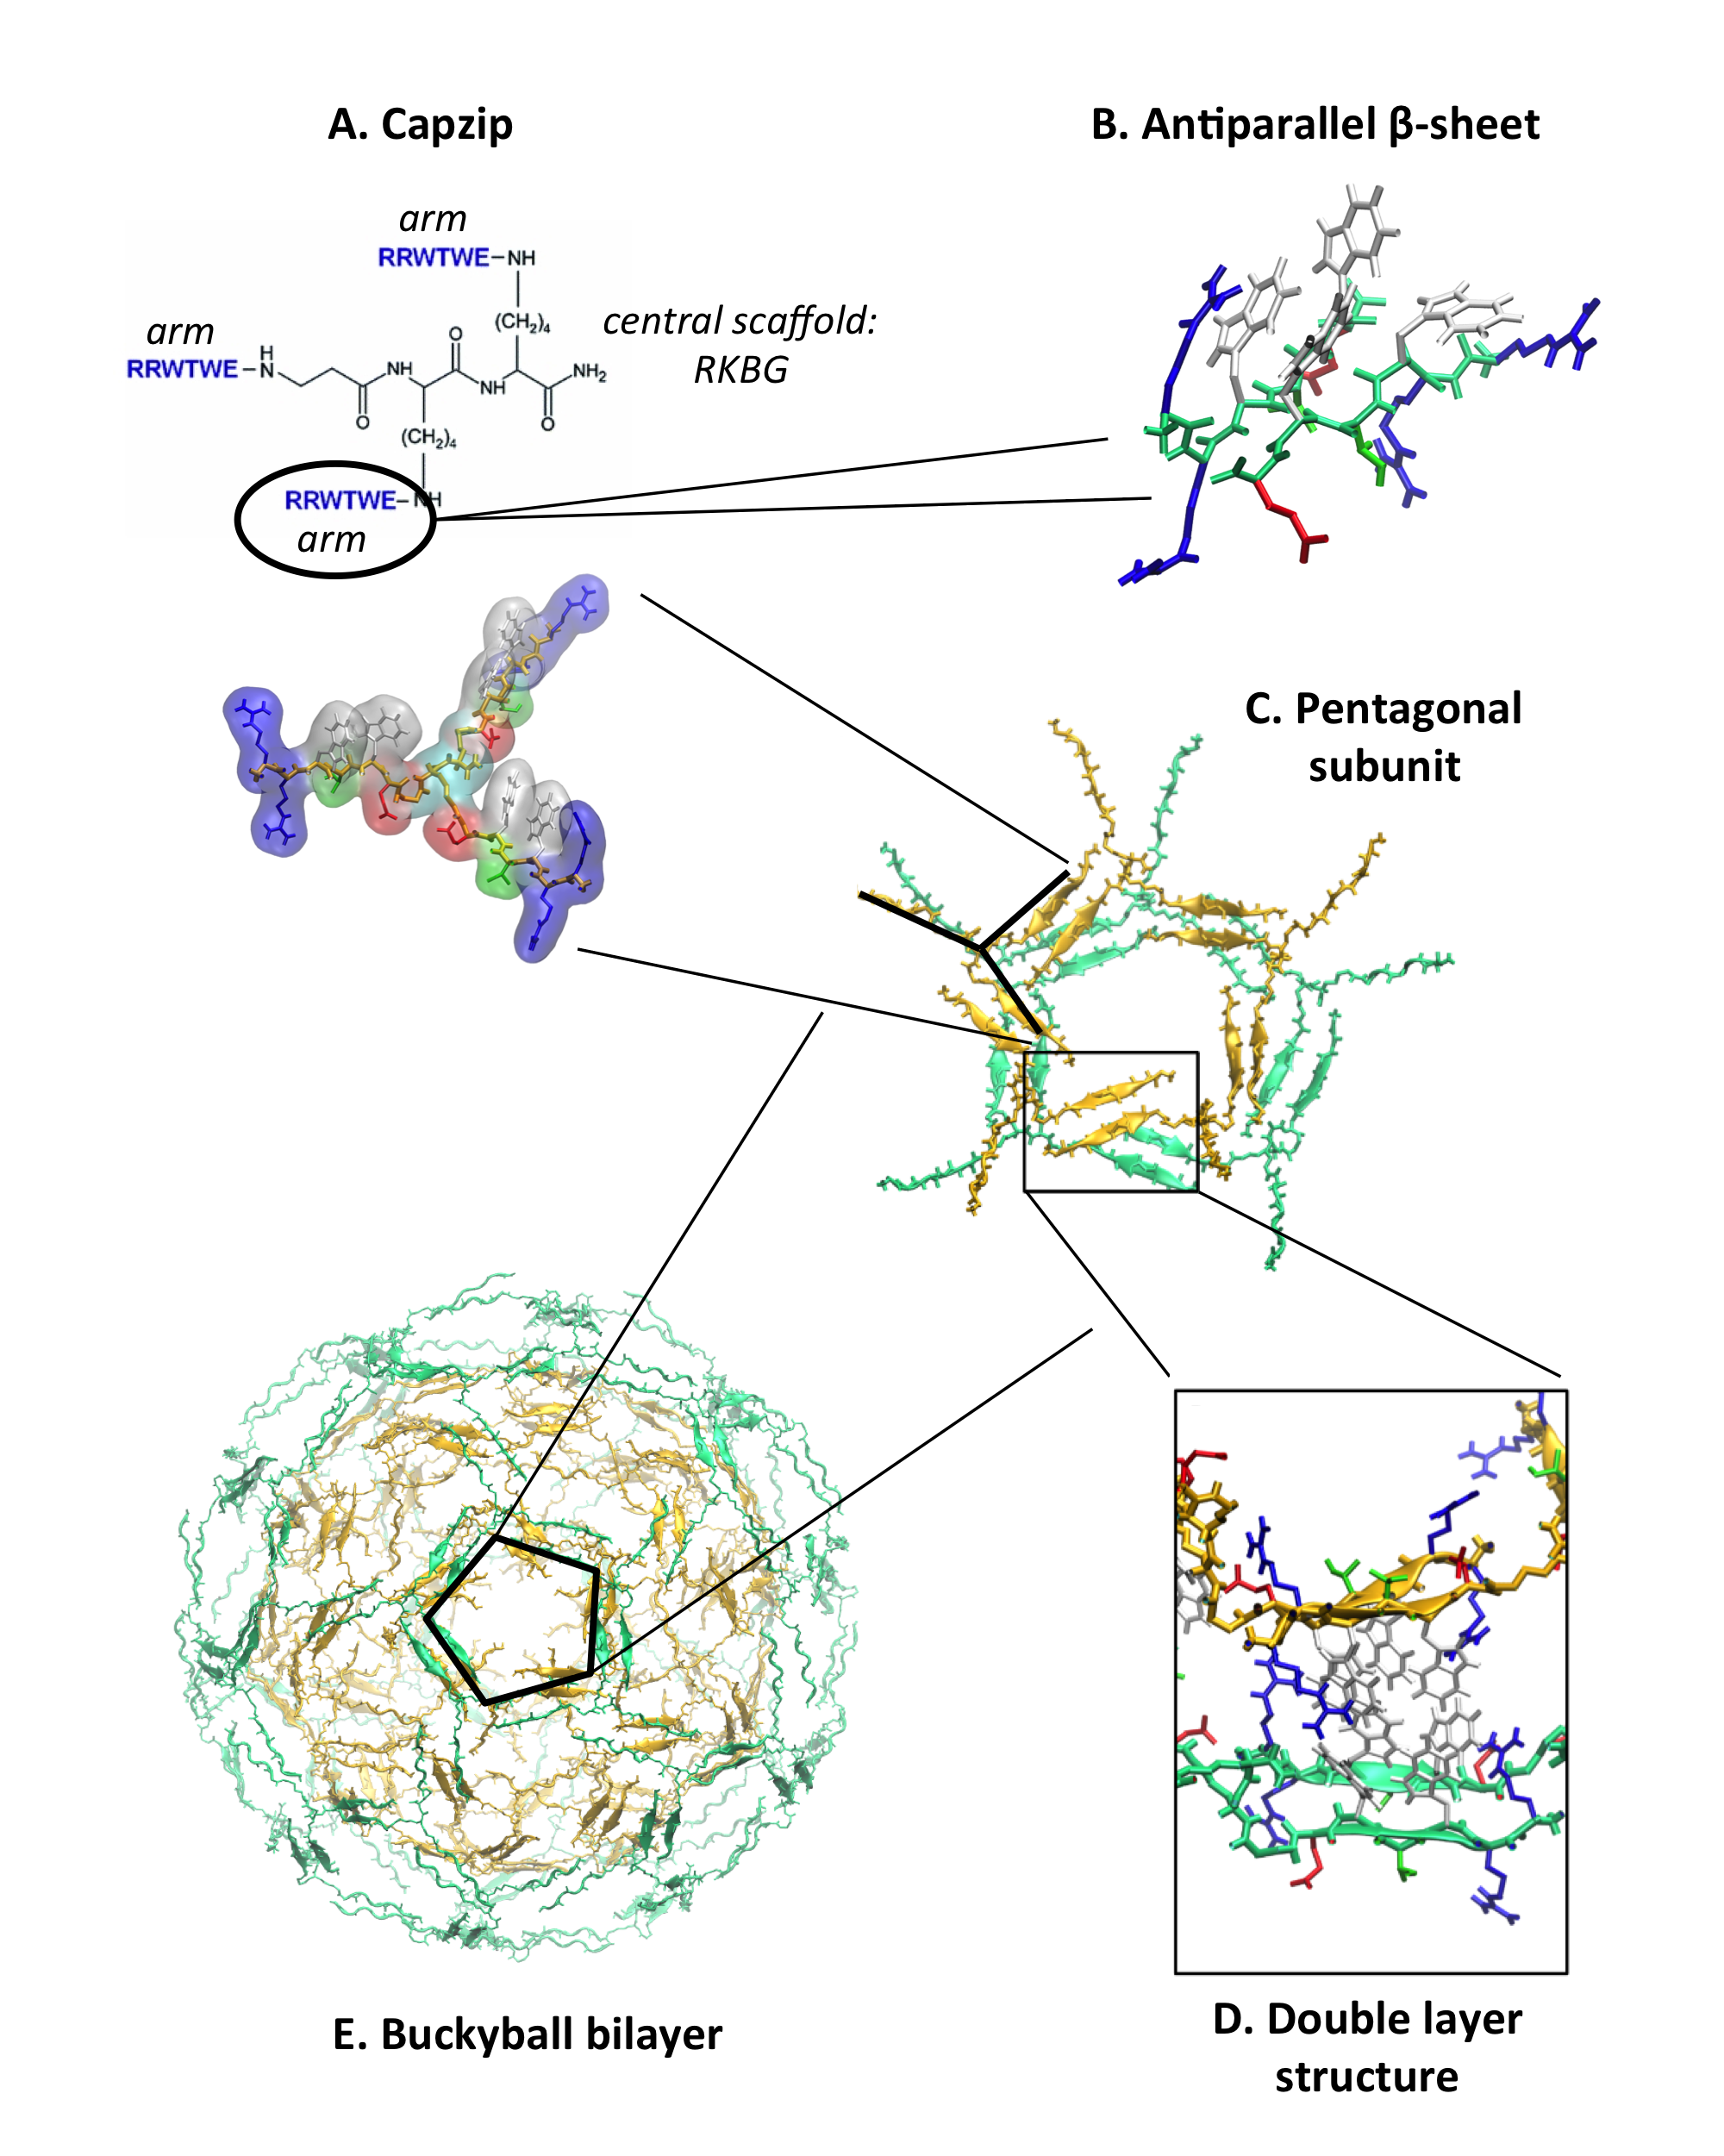
\includegraphics[width=0.95\linewidth]{3results_capsule/pics/img_build.png}
\caption[Building blocks of capzip assembly]{A. Capzip molecule: formula, with arms in blue characters and central scaffold (residue RKGB) in black lines; and bonds/surface representation, with surface color coded by amino acid type (blue positive, green polar, red negative, white hydrophobic).
%
B: detail of two arms paired in an antiparallel $\beta$-sheet (bond and cartoon representation, backbone in green and side chain color coded by amino acid type).
%
C: pentagonal subunit (bonds and cartoon representation, green and yellow for the two different layers): ten antimicrobial molecules arranged in two stacking pentagons. 
%
D: detail of the double layer of each pentagonal subunit (bonds representation of side chains is color coded by amino acid type, and backbone in cartoon representation, green and yellow for the two different layers).
%
E: atomistic structure of the buckyball bilayer simulated (bonds and cartoon representation of backbone only, green outer layer, yellow inner layer). [VMD software, \citet{HUMP96}]}
\label{fig:BTI_vmd}
\end{figure}



\section{Modelling the assembly} \label{sec:build}

\paragraph{Subunits simulations} As previously mentioned, the antimicrobial sequence of capzip is designed with opposite charges at its extremes to favour an antiparallel $\beta$-sheets pairing with other copies of itself (Figure \ref{fig:BTI_vmd}, A-B).
%
MD simulations of two RRWTWE sequences paired in this fashion (Figure \ref{fig:BTI_vmd}, B) confirm that the assembly is stabilised by the interactions between opposite charges (statistics gathered over 16 replicas, each run for 20 ns).
%
Moreover, backbone hydrogen bonds form between Tryptophan residues of facing strands, after a shift of the mutual positions of the chains which brings Tryptophans in front of each other (see the scheme in Figure \ref{fig:hb_beta_SIhere_hb}).
%
Finally, $\pi$-stacking interaction (parallel or T-shaped) between Tryptophan side chains contributes to the interaction as well, albeit in minor measure (Figure \ref{fig:hb_beta_SIhere_pi1}-\subcaptionref{fig:hb_beta_SIhere_pi2}; details on the computation are explained in Section \ref{sec:analysis}). The T-shaped orientation is favoured with respect to a parallel stacking, consistently with the fact that the latter produces an unfavourable repulsion between the planar faces of the rings \citep{Hunter2001}.  
%
Thus, Tryptophan residues dictate the interdigitation of facing residues in the two chains.
%
\begin{figure}
\centering
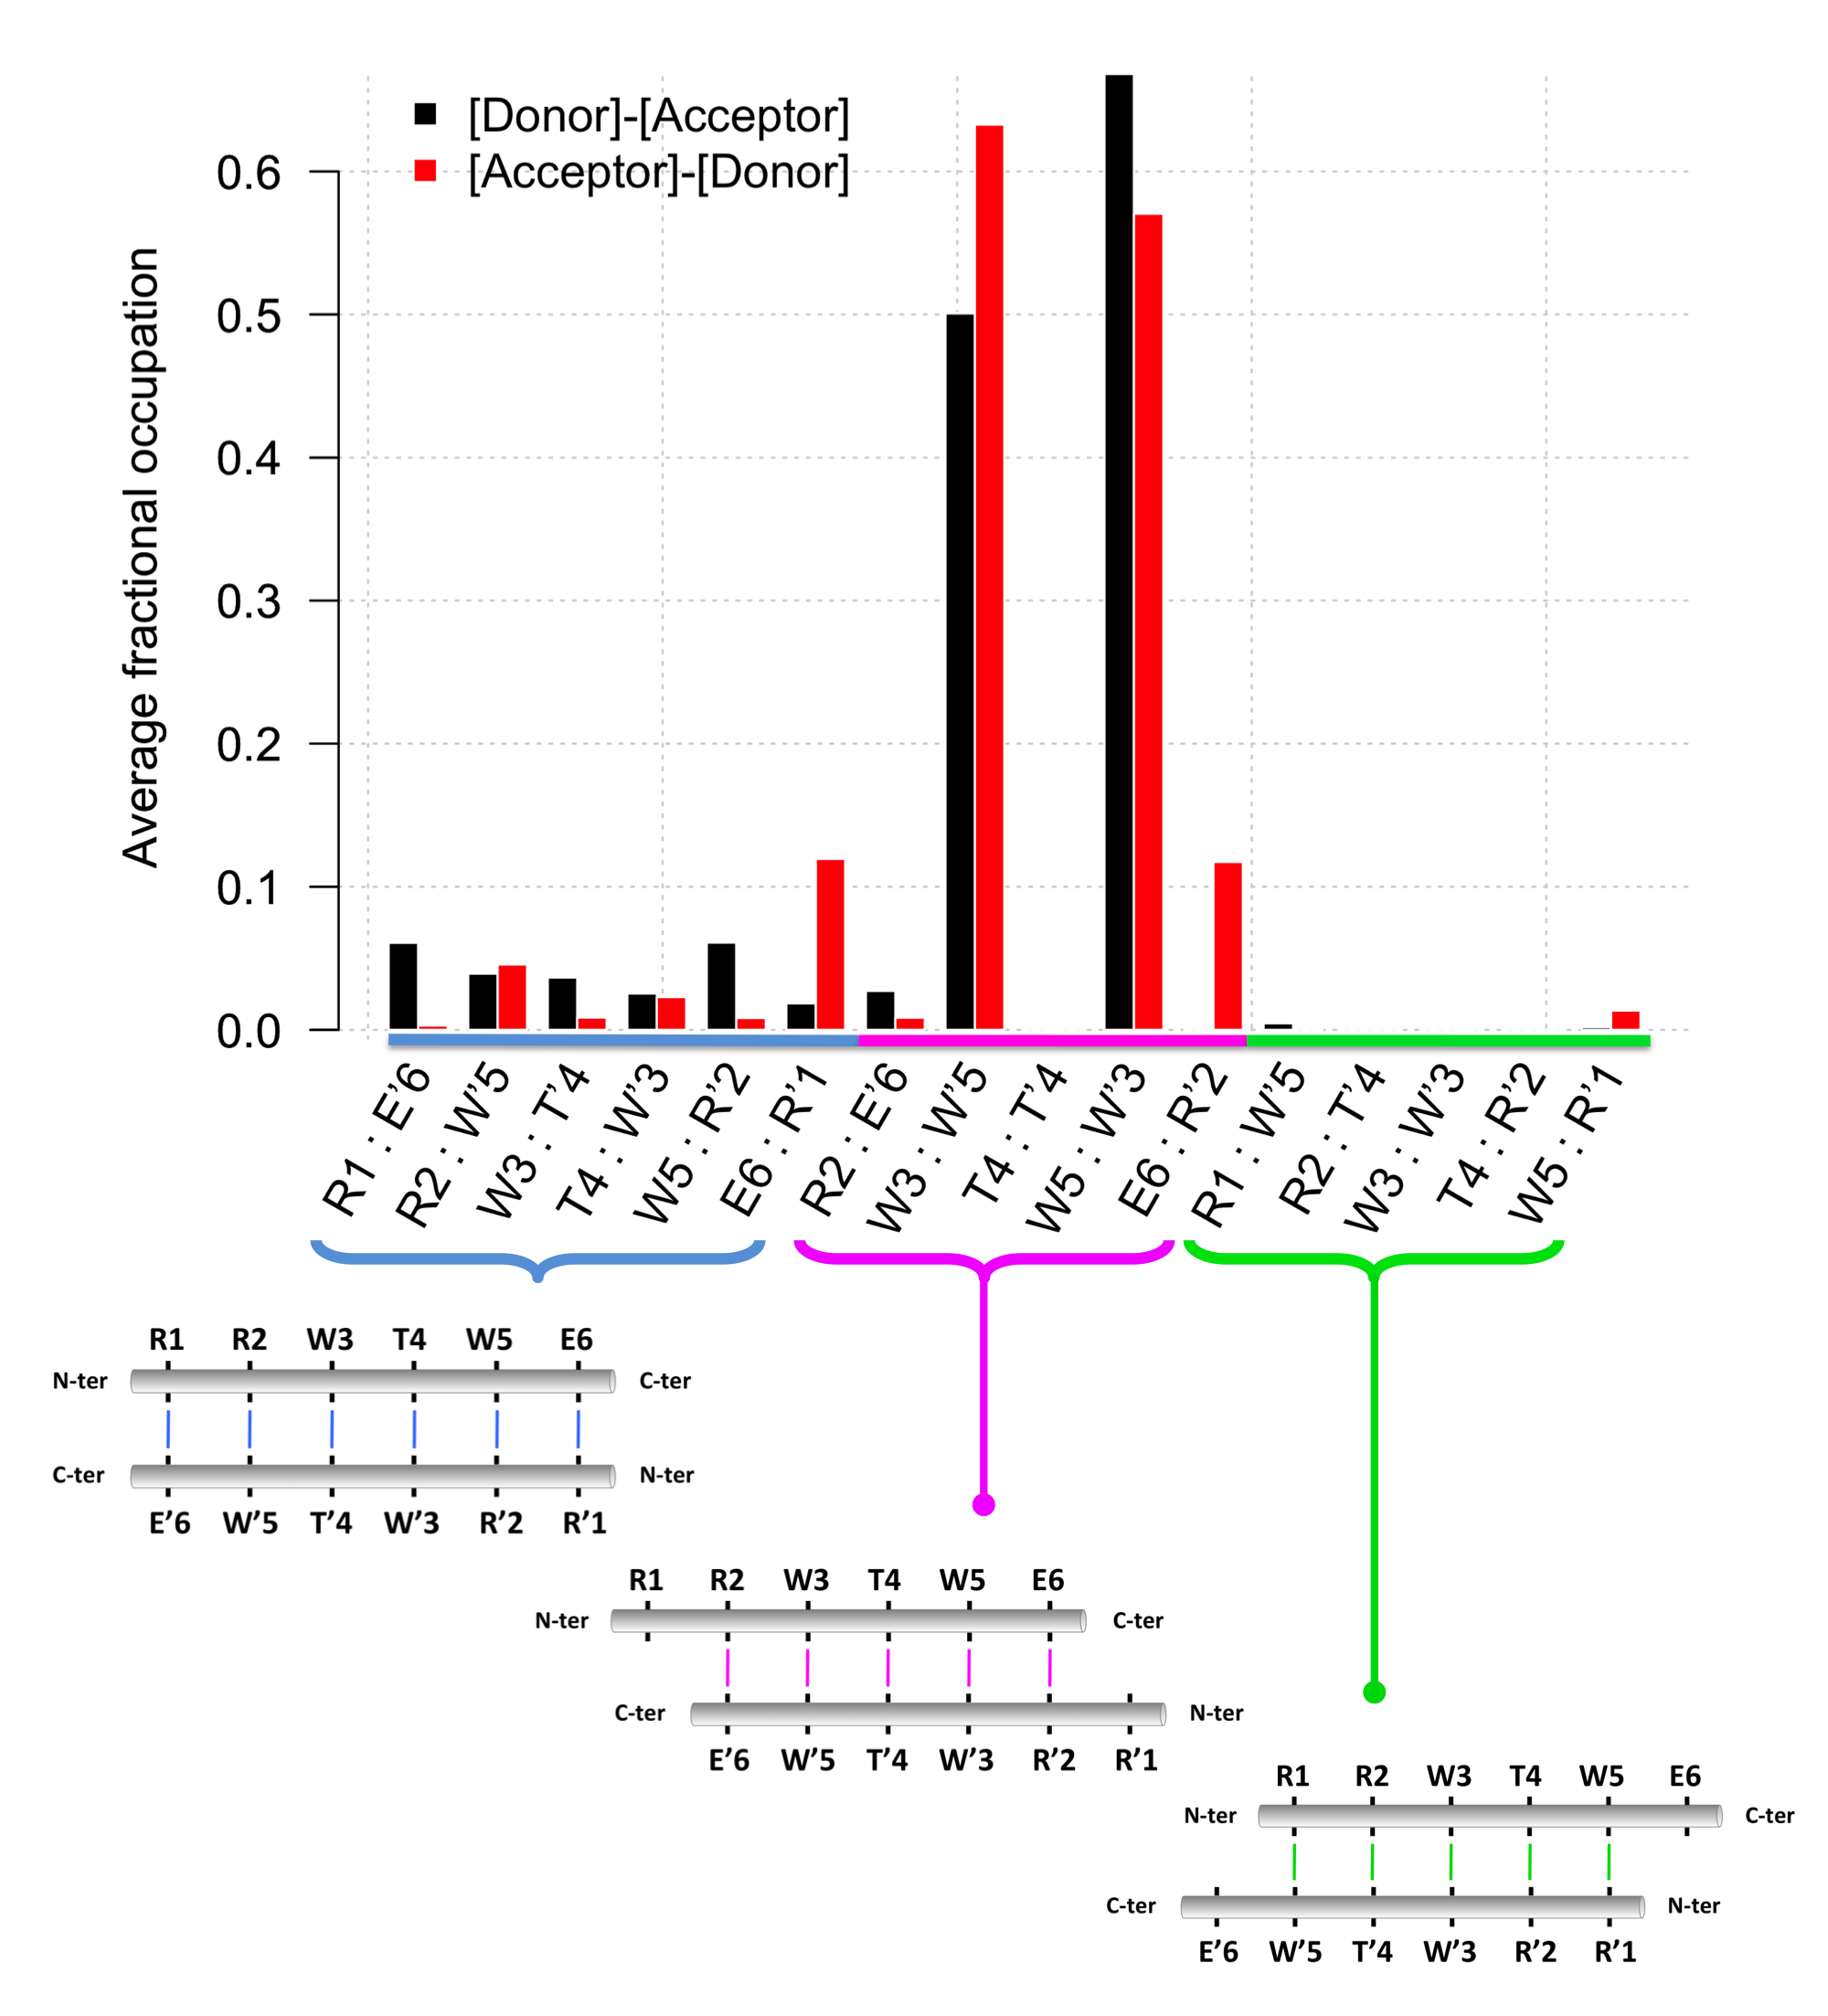
\includegraphics[width=0.9\linewidth]{3results_capsule/pics/merged_figures_beta_sheet2}
\caption[Hydrogen bonds in a RRWTWE $\beta$-sheet]{Presence of backbone hydrogen bonds between two facing antiparallel RRWTWE chains. The pairs highlighted in blue, green and pink corresponds to three different chains arrangements, shown in the schemes below the histogram. Bonds are labelled by amino acid pairs, named as in the schemes and underlined with matching color; occupancy is averaged over 16 simulations of 20 ns each.}
\label{fig:hb_beta_SIhere_hb}
\end{figure}

\begin{figure}[p!]
\centering
\subbottom[]{%
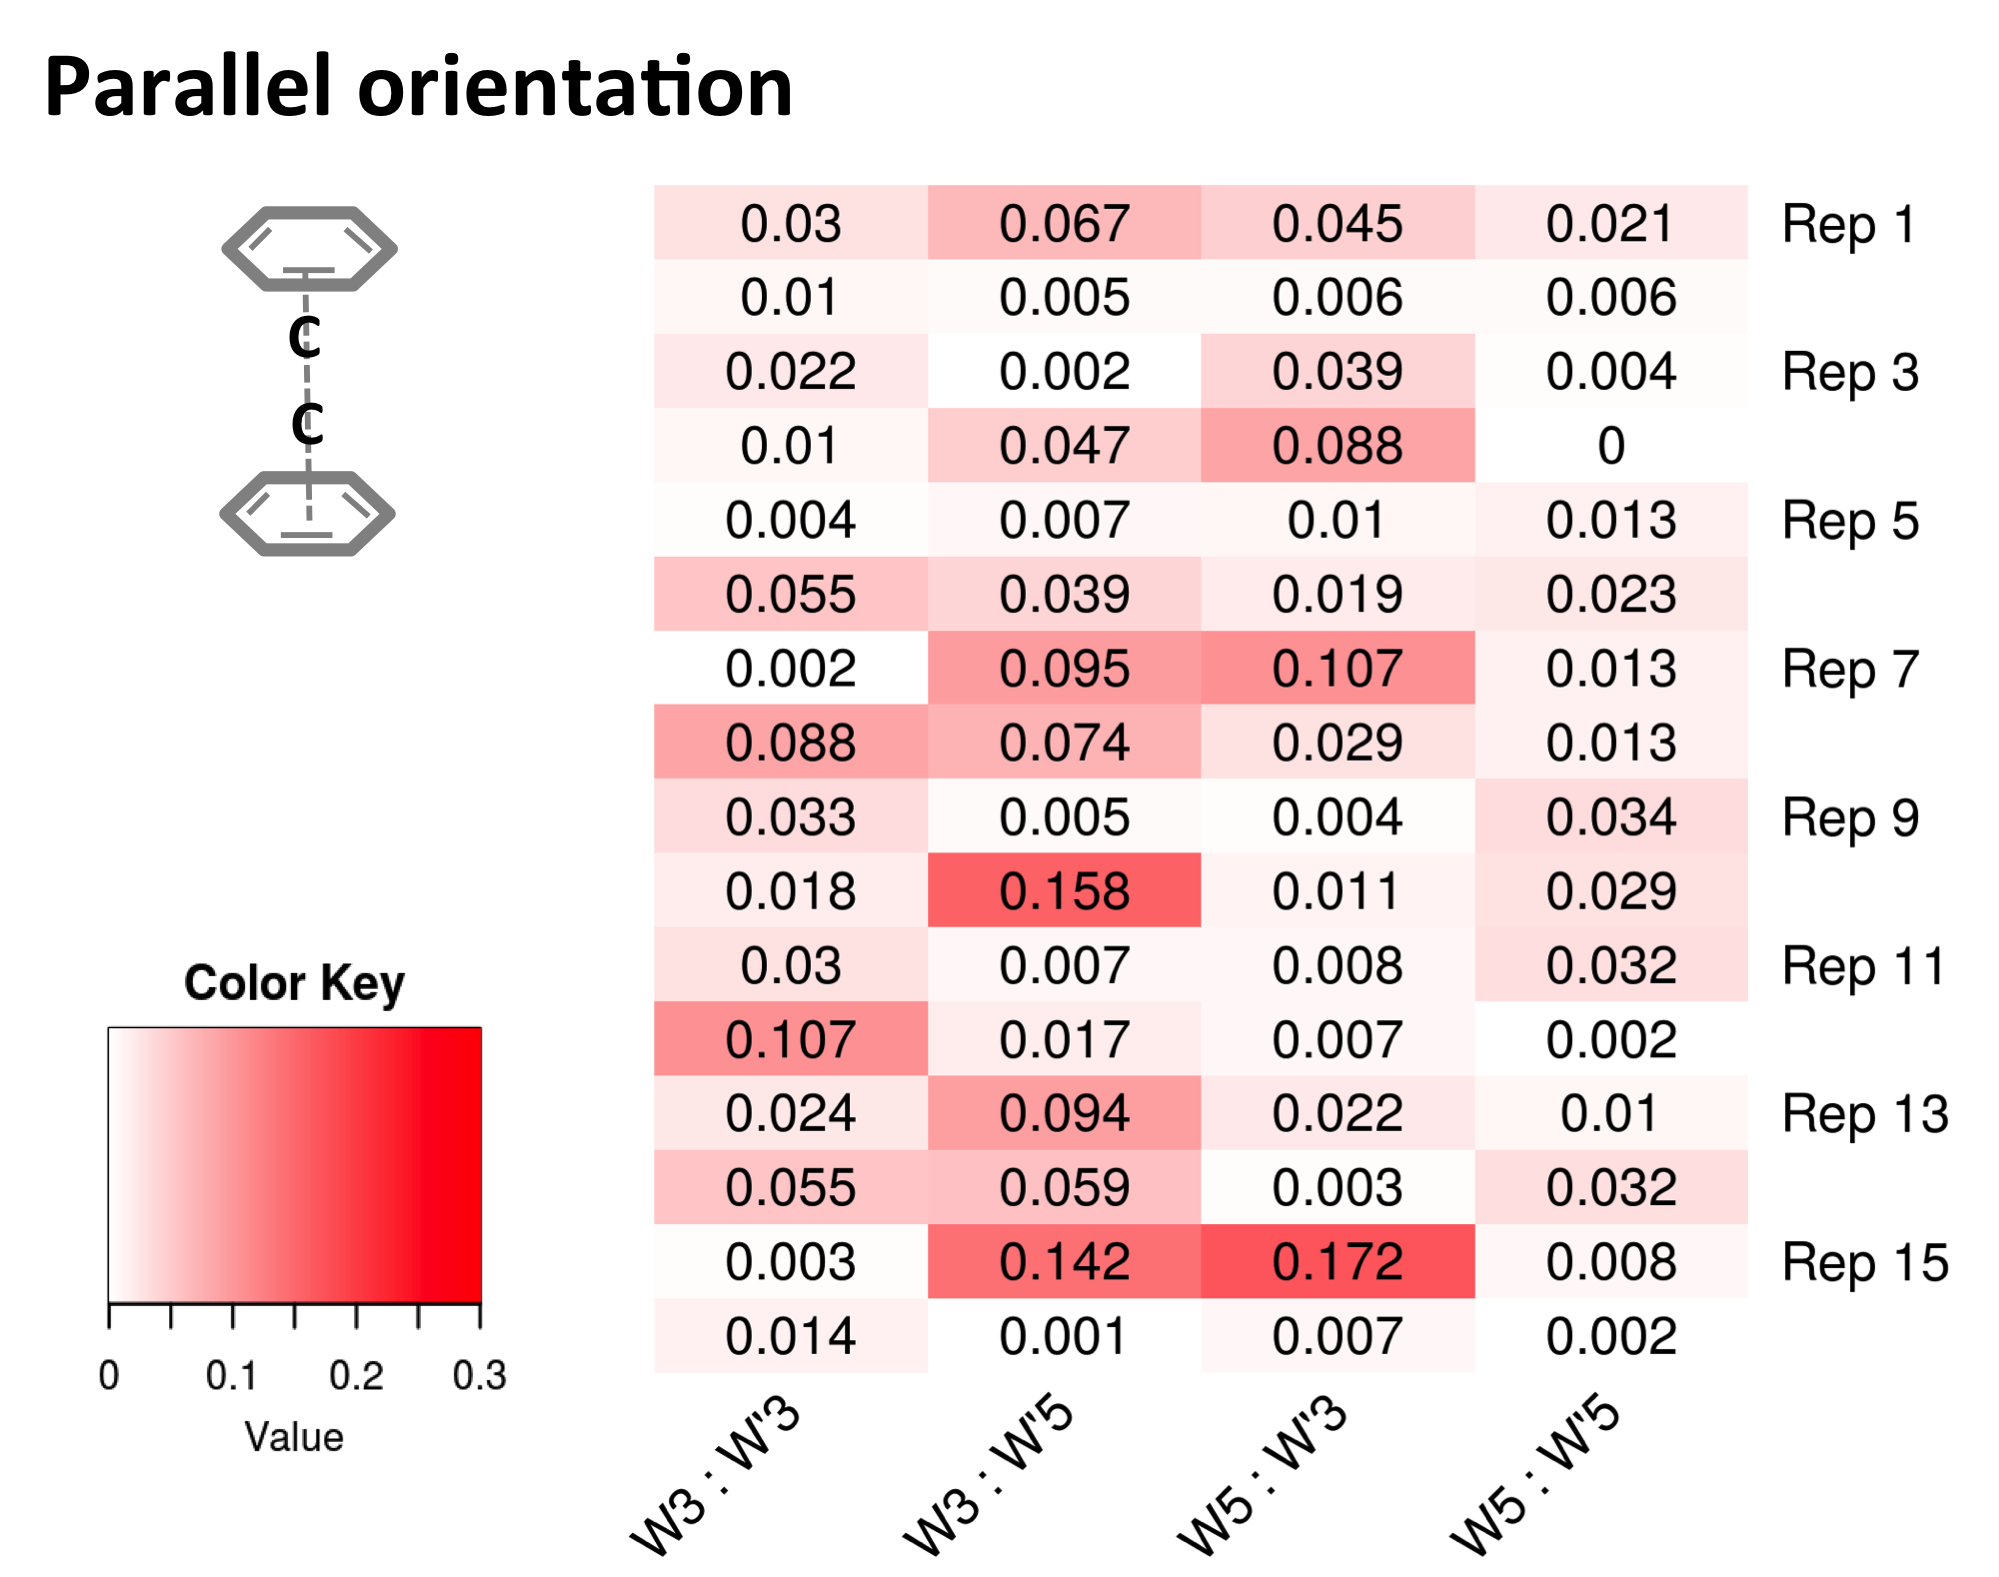
\includegraphics[width=0.75\linewidth]{3results_capsule/pics/pi_stacking_0} \label{fig:hb_beta_SIhere_pi1}} \hspace{0.2cm}
\subbottom[]{%
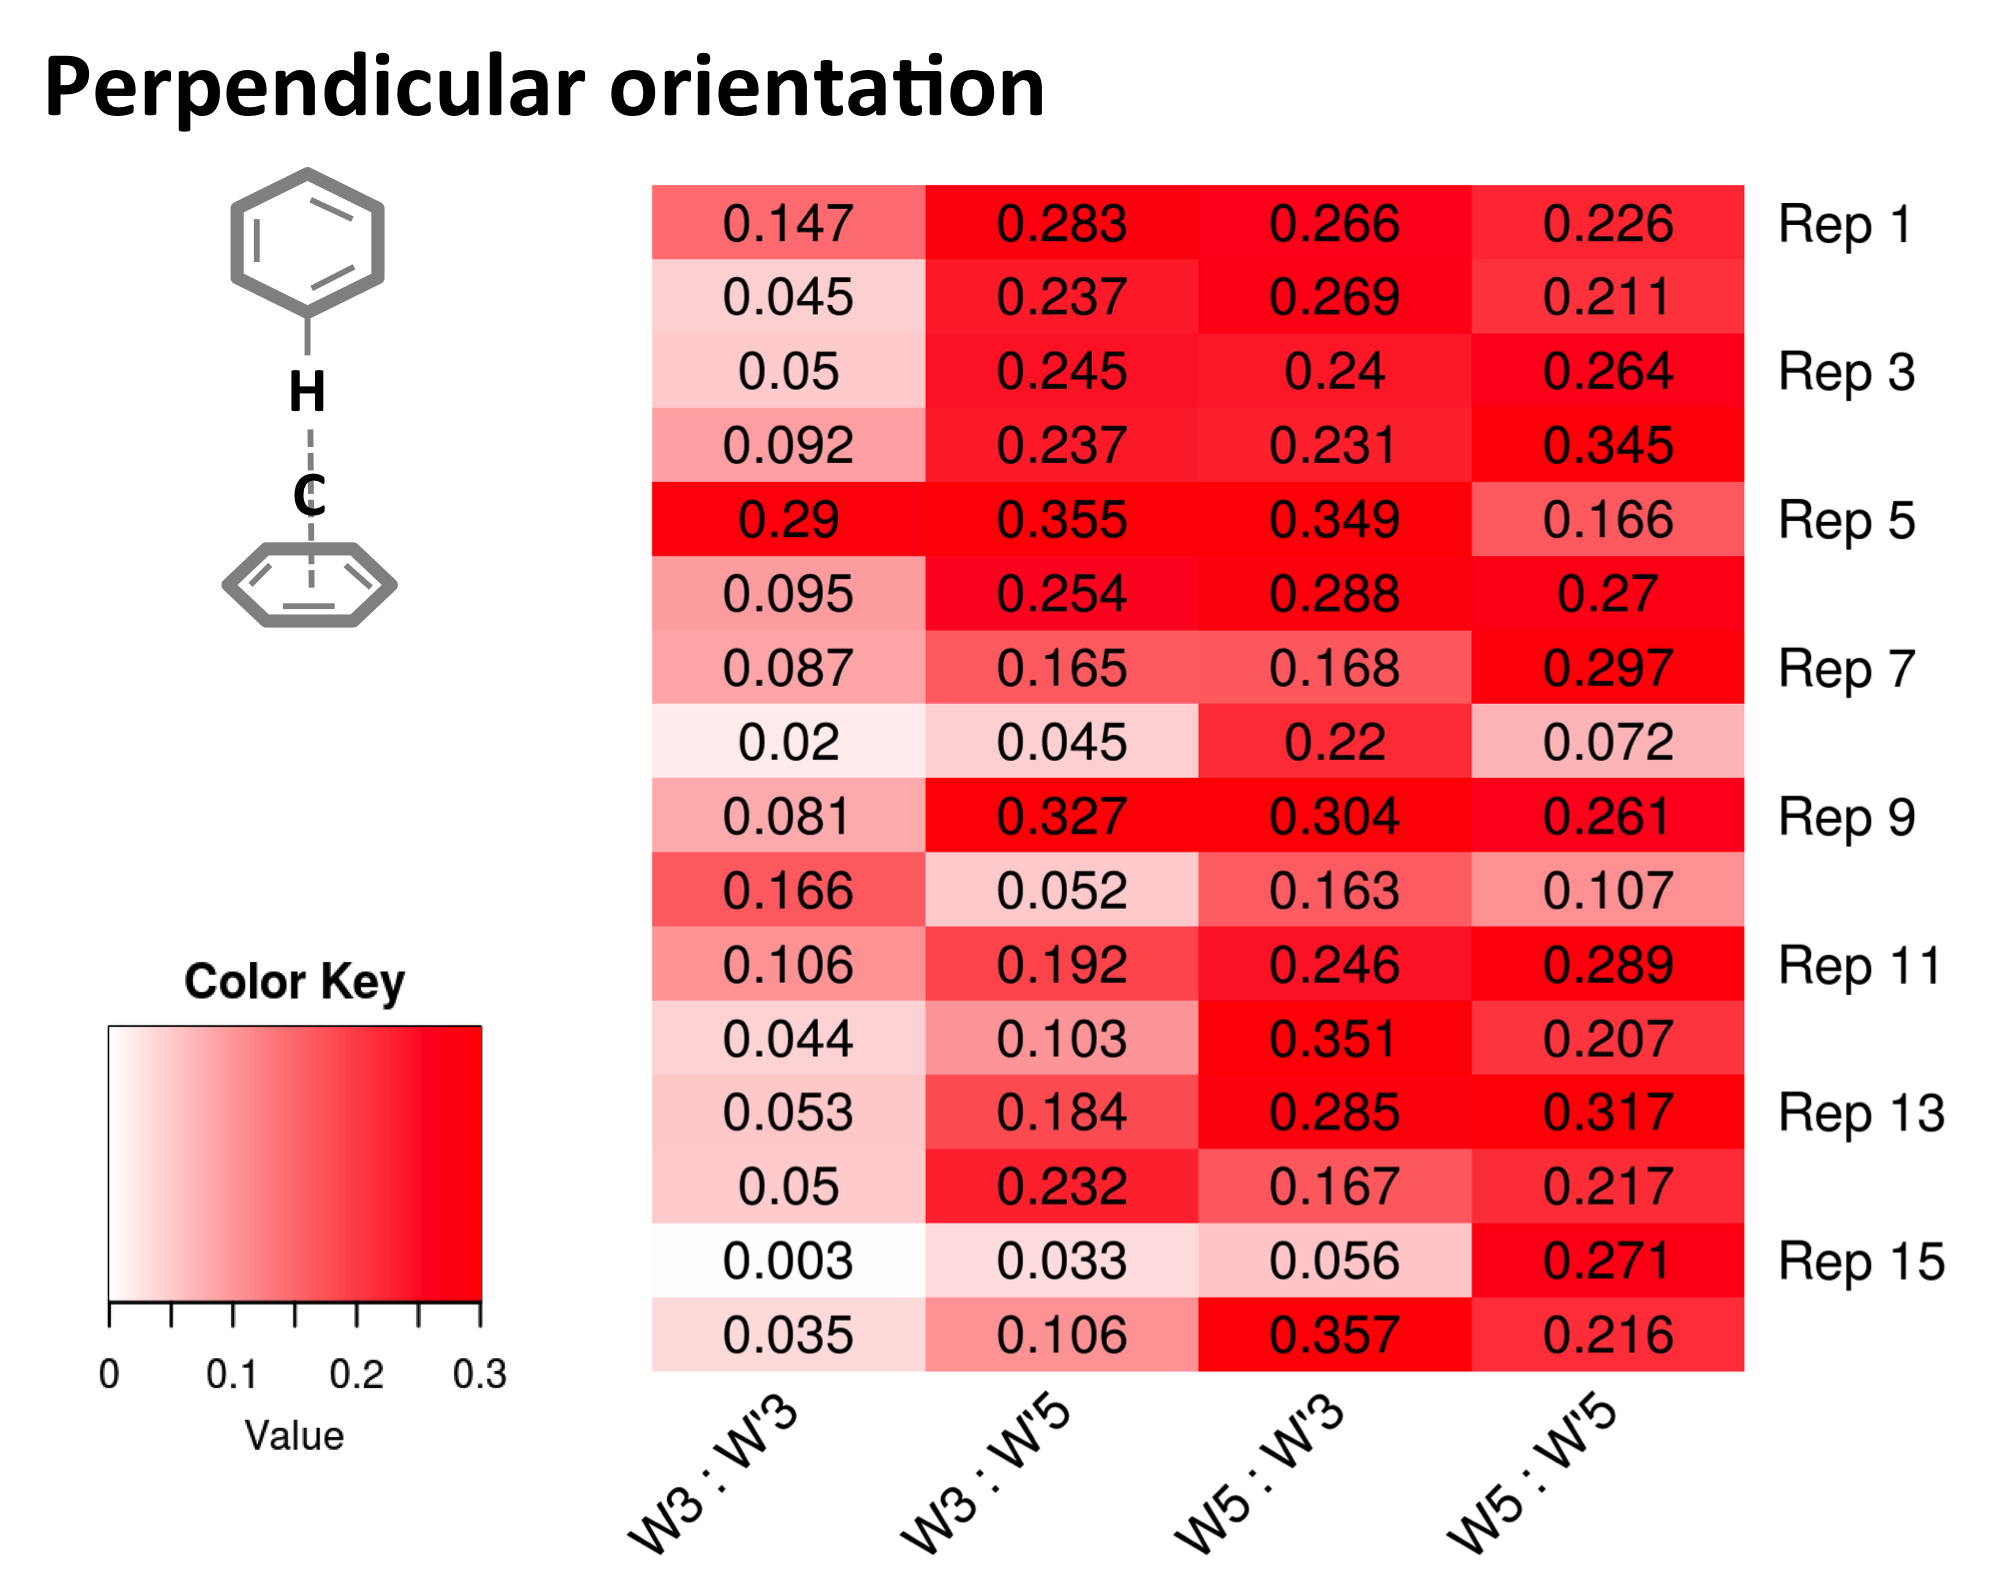
\includegraphics[width=0.75\linewidth]{3results_capsule/pics/pi_stacking_90} \label{fig:hb_beta_SIhere_pi2}}
\caption[$\pi$-stacking interaction in a RRWTWE $\beta$-sheet]{Presence of parallel or T-shaped $\pi$-stacking between each possible pair of facing Tryptophan residues in two RRWTWE chains arranged in an antiparallel $\beta$-sheet. For each replica the map gives the fraction of time for which a parallel or T-shaped $\pi$-stacking interaction has been observed (total simulation time 320 ns).}
\label{fig:hb_beta_SIhere}
\end{figure}

Analogous simulations of two RRWTWE sequences paired in a parallel way show loosening of the pairing and in some cases the flip of one sequence to rearrange with respect to the other in the antiparallel manner, confirming that the antiparallel arrangement is favoured.

The hydrophobic interactions between Tryptophan residues (in white in Figure \ref{fig:BTI_vmd}, B) results in the creation of a hydrophobic patch which includes four of them on one side of the $\beta$-sheet plane.
%
This generates an amphiphilic structure where the hydrophobic core is segregated from the remaining charged residues distributed around.
%
The combination of two stacking $\beta$-sheets, paired to match their hydrophobic patches, constitutes an effective supramolecular assemblies to reduce the solvent exposure of such residues (Figure \ref{fig:BTI_vmd}, D).

\paragraph{Oligomer simulations} This pairing strategy, however, needs to be applied in the context of assembly of complete molecules, i.e.\ three arms joined by the central scaffold. From now on, we will denote the central scaffold as RKGB residue. This was the name given to the moiety by the ATB server \citep{Malde2011, Koziara2014} used to compute its atomistic parameters (see Section \ref{sec:details}).
%
The quasi three-fold symmetry of capzip suggests a regular geometric arrangement; at the same time simulations of a single molecule in solution highlight its flexibility, proposing that multiple arrangements can be accommodated by the molecule.
%
The best examples of geometrically organised protein structures can be found in viral capsids, which are composed by the regular repetition of highly symmetric protein subunits.
%
Inspired by this, we tested whether a geometrical organisation can represent a stable capsule, choosing as minimal representative geometry a truncated icosahedron (buckyball, Figure \ref{fig:BTI_vmd}, E). This shape has 12 pentagonal faces and 20 hexagonal ones.

Preliminary atomistic simulations (100 ns) were run on a pentagonal subunit (Figure \ref{fig:BTI_vmd}, C), where ten antimicrobial molecules are arranged in two stacking pentagons. Capzip arms are paired in antiparallel $\beta$-sheets to form each pentagon, and the two of them are facing with their Tryptophan residues in contact (Figure \ref{fig:BTI_vmd}, D).
%
The simulations proved the cohesion between molecules belonging to the subunit. Specifically, the number of contacts between backbone $C^\alpha$s augmented slightly in the first 20 ns (Figure \ref{fig:penta_results_here_1}), due to the compaction of the unpaired external arms toward the core of the structure (see Supplementary Figure \ref{fig:penta_results_SI}), which made the Coulomb energy decrease.
%
Moreover, for each pair of facing chains (see definition in Figure \ref{fig:penta_results_here_2}), we computed the distance between their centres of mass. Figure \ref{fig:penta_results_here_2} reports the variance of these distances normalised by their average value, as a measure of the cohesion of the subunit, showing that in the majority of the cases less than 2\% of variability is observed. Overall, the block is not rigid, and does indeed deform and go back to the pentagonal shape multiple times in the simulation, but it is keeping the original pairing of the molecules.
% RUN SECOND SIMULATION?
\begin{figure}[t!]
\centering
\subbottom[]{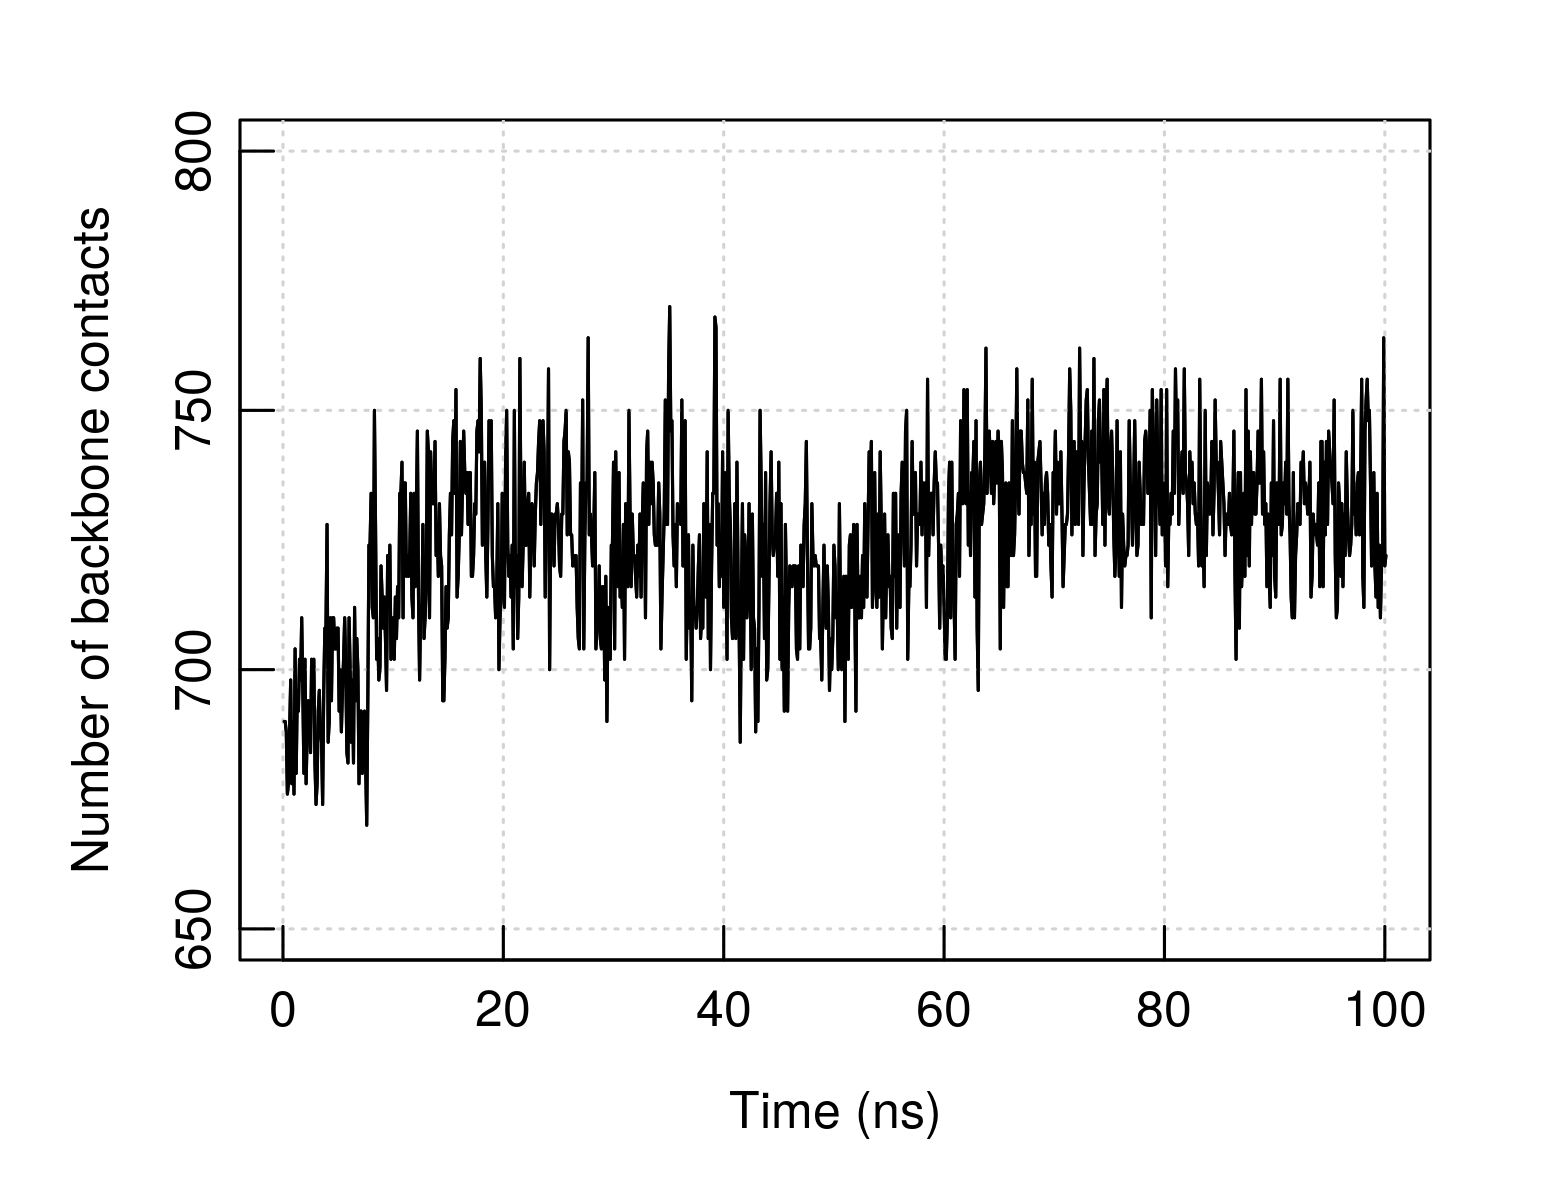
\includegraphics[width=0.48\linewidth]{3results_capsule/pics/bb_contacts.png} \label{fig:penta_results_here_1}}
\subbottom[]{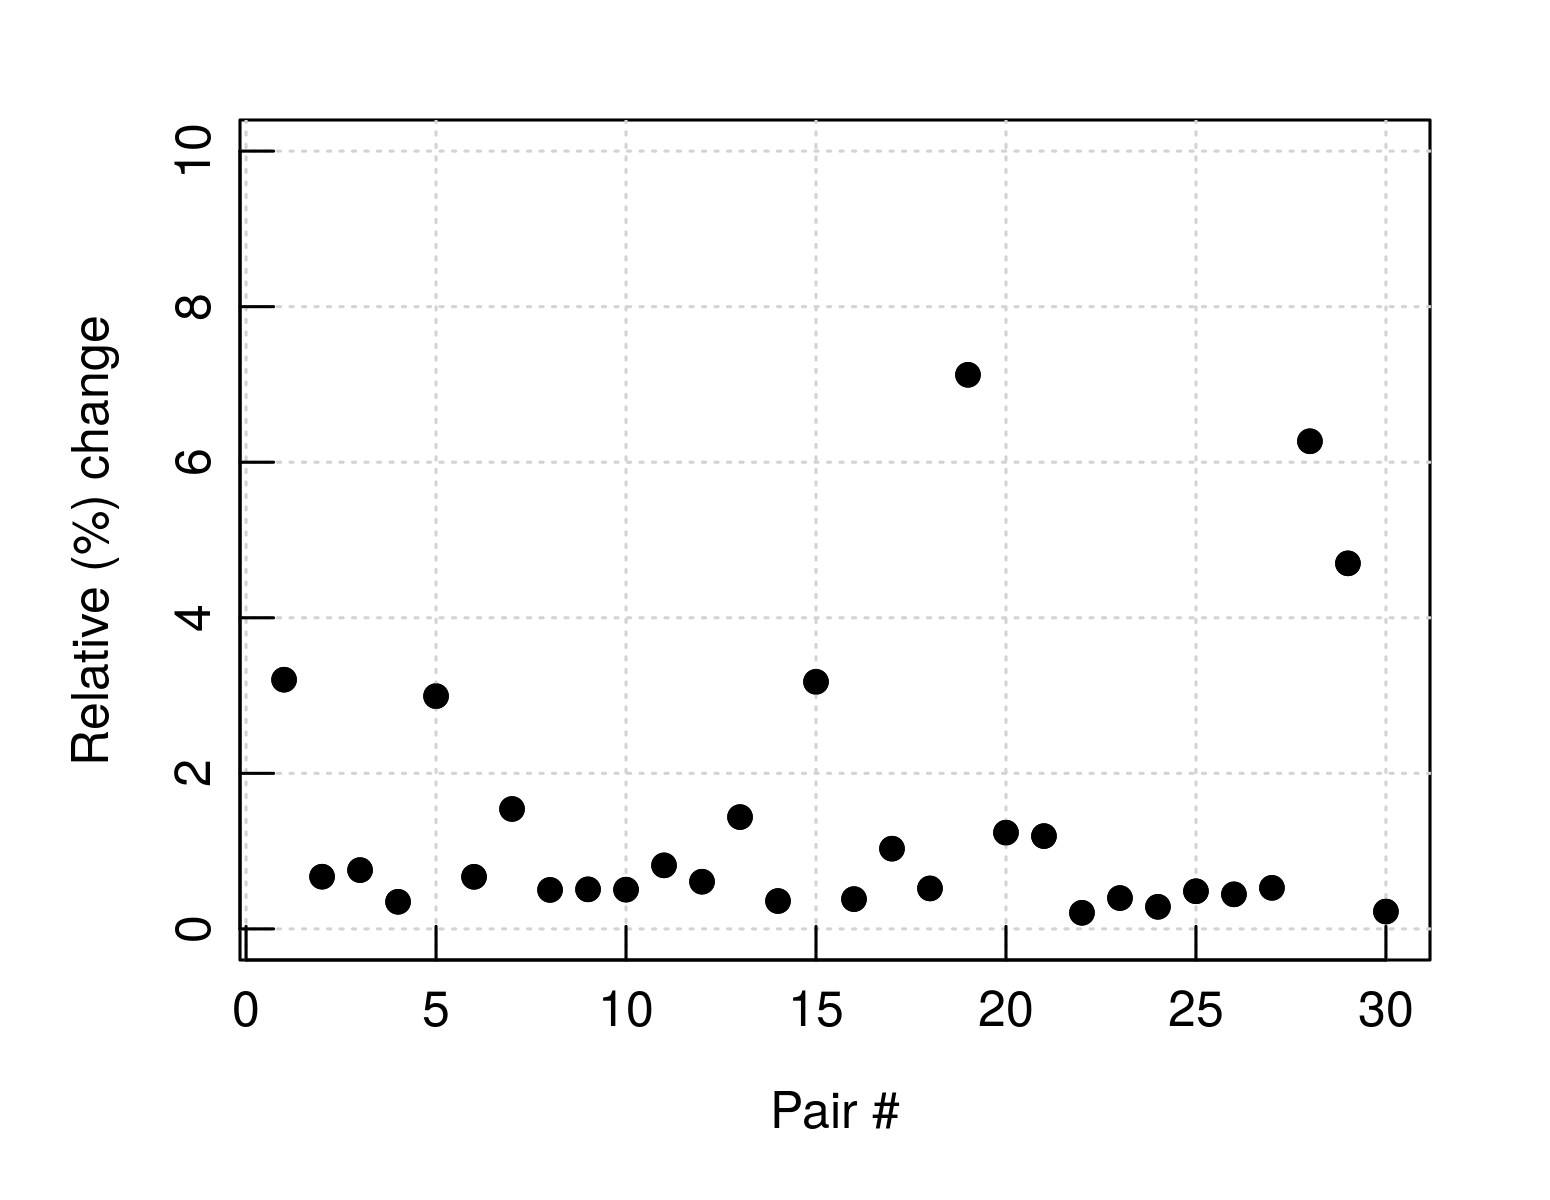
\includegraphics[width=0.48\linewidth]{3results_capsule/pics/chain_COM_distance.png} \label{fig:penta_results_here_2}}
\caption[Cohesion measures on the pentagonal subunit]{(a) Number of backbone contacts during a simulation of a pentagonal subunit. (b) Variability of the inter chain average distance between the 30 facing chains in the pentagon. The 30 pairs defined as facing are the chains belonging to the same $\beta$-sheet (5 for each of the two stacking pentagons), and for each stacking $\beta$-sheet the 4 possible inter-pentagon (inter-layer) pairs of chains.}
\label{fig:penta_results_here}
\end{figure}

\paragraph{Capsule simulations} The pentagonal subunit respects the building principles of $\beta$-sheet pairing between antimicrobial sequences. Moreover, the double layer structure allows to partially screen the hydrophobic residues from the solvent, as they are in favourable contact with each other (Figure \ref{fig:BTI_vmd}, D).
%
Twelve of these units can be used to build a truncated icosahedron (Figure \ref{fig:BTI_vmd}, E): they constitutes its pentagonal faces, while the hexagonal ones are formed when the arms extending from the pentagons join together.

Each capzip molecule is centred in one vertex of the polygon, with the arms laying alongside the edges departing from it. On each edge two arms coming from opposite sides meet in an antiparallel fashion.
%
The full truncated icosahedron (Figure \ref{fig:BTI_vmd}, E) has two concentric layers, for a total of 120 molecules, and initial radius of 7.7 nm. Thus it will be called \emph{buckyball bilayer} in the following.
%
As anticipated, this geometry represents a minimal model of the possible structures capzip adopts in solution.

The structure was simulated at atomistic and coarse-grained levels, respectively with the GROMOS 53A6 \citep{Oostenbrink2004}, SIRAH \citep{Machado2018} and MARTINI \citep{Marrink2007, Monticelli2008} force fields (with both standard and polar water \citep{Yesylevskyy2010}).
% LEAVE?
From the final configurations of the MARTINI coarse-grained model (standard water), atomistic coordinates were obtained and simulated, to be compared with the original atomistic dynamics.
%
Moreover, additional simulations were run at all the coarse-grained levels on a buckyball monolayer (i.e.\ built from pentagonal subunits made by one pentagon only), to prove whether the bilayer is more energetically favoured.

Finally, a test study on self-assembly was performed with one of the coarse-grained representations (MARTINI with standard water), starting from capzip molecules randomly placed in solution.

\paragraph{Capzip-membrane simulations} A multiscale analysis is needed also to investigate the antimicrobial activity. Being highly costly to simulate the buckyball bilayer on a membrane at the atomistic level, the pentagonal subunit employed to build the complete structure (Figure \ref{fig:BTI_vmd}, C) was taken as representative of the latter. It was simulated parallel to the membrane plane, with its center of mass at 1.5 nm from the phosphate plane (Figure \ref{fig:pL6_vmd_1}), to avoid spending time in sampling conformations with the peptide far from the membrane. This, together with a tailored use of an applied electric field (see Section \ref{sec:details}), speeds up simulations considerably.
%
To observe the natural binding of the peptide to the membrane, the process of the buckyball bilayer approaching a model membrane was simulated with a MARTINI coarse-grained description (Figure \ref{fig:pL6_vmd_2}). The use of the MARTINI polar water \citep{Yesylevskyy2010} allowed for the introduction of an external electric field, to compare the coarse-grained simulations with the atomistic ones which employ analogous conditions.

% TRUE ONLY IF COMPLETED DPPC
Two membrane compositions were simulated for both resolutions, a model bacterial and a model mammalian membrane, to identify the different interactions with the peptide. The first one presents 25\% of anionic lipids (DLPG), and the remaining zwitterionic (DLPC), while the second has only DLPC lipids. The choice of the bacterial model was dictated by the experiments performed on capzip \citep{Castelletto2016}, and the mammalian one was built with the same zwitterionic lipid as for the bacterial to simplify the comparison, e.g.\ to have membranes with comparable thickness and mechanical properties.

\begin{figure}[t]
\centering
\subbottom[]{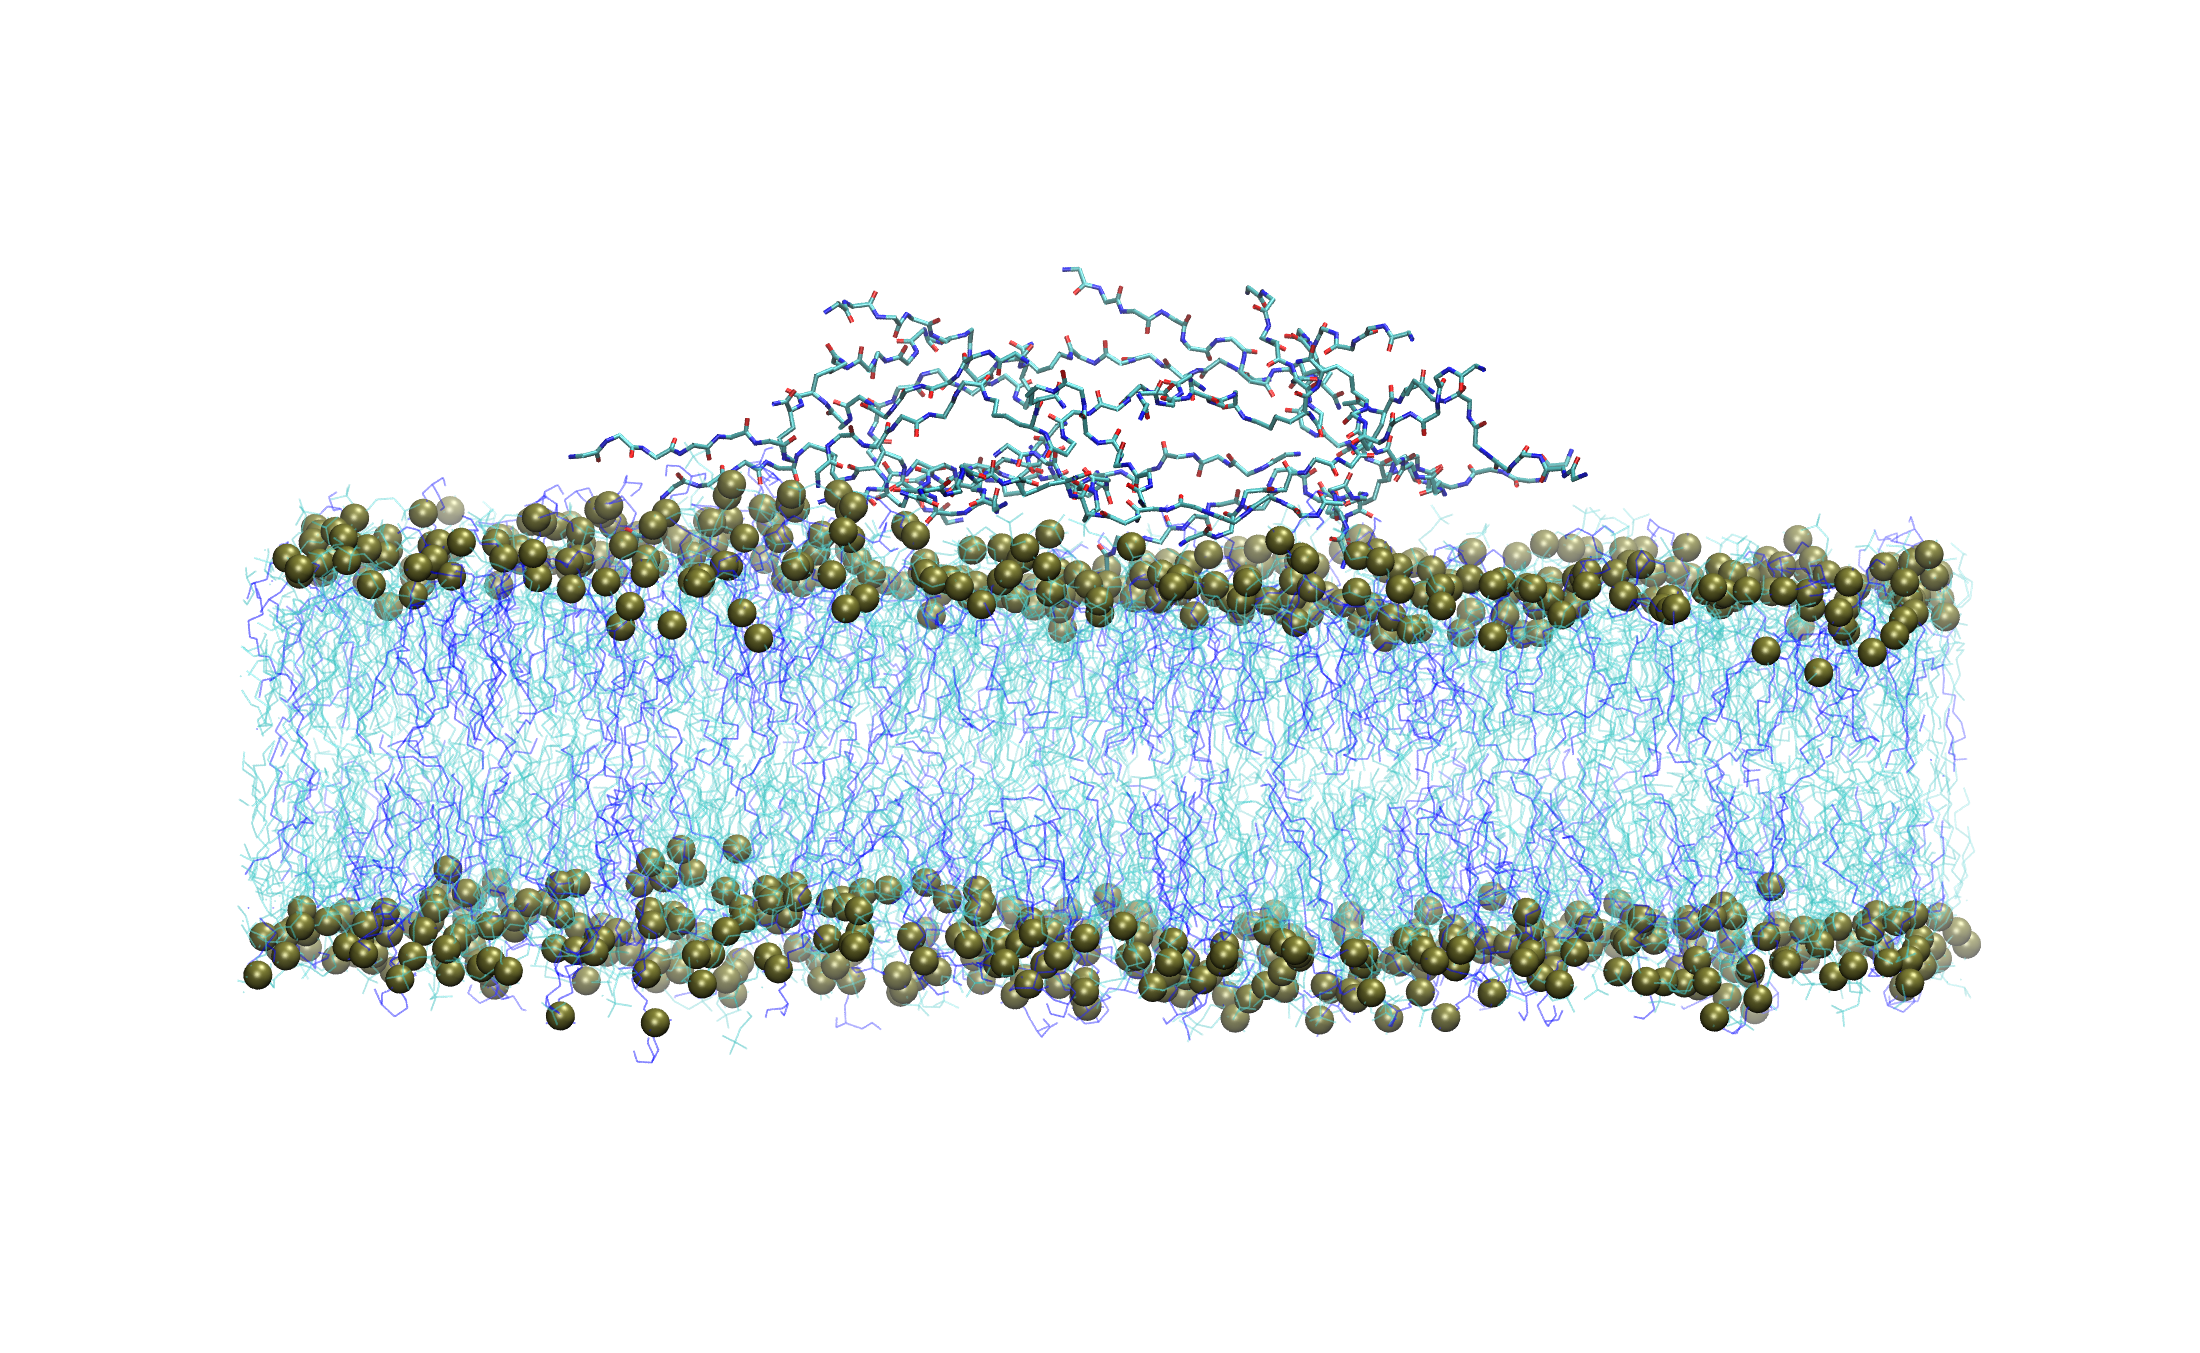
\includegraphics[width=0.45\linewidth]{3results_capsule/pics/pL6_Pramp_pic2.png} \label{fig:pL6_vmd_1}}
\subbottom[]{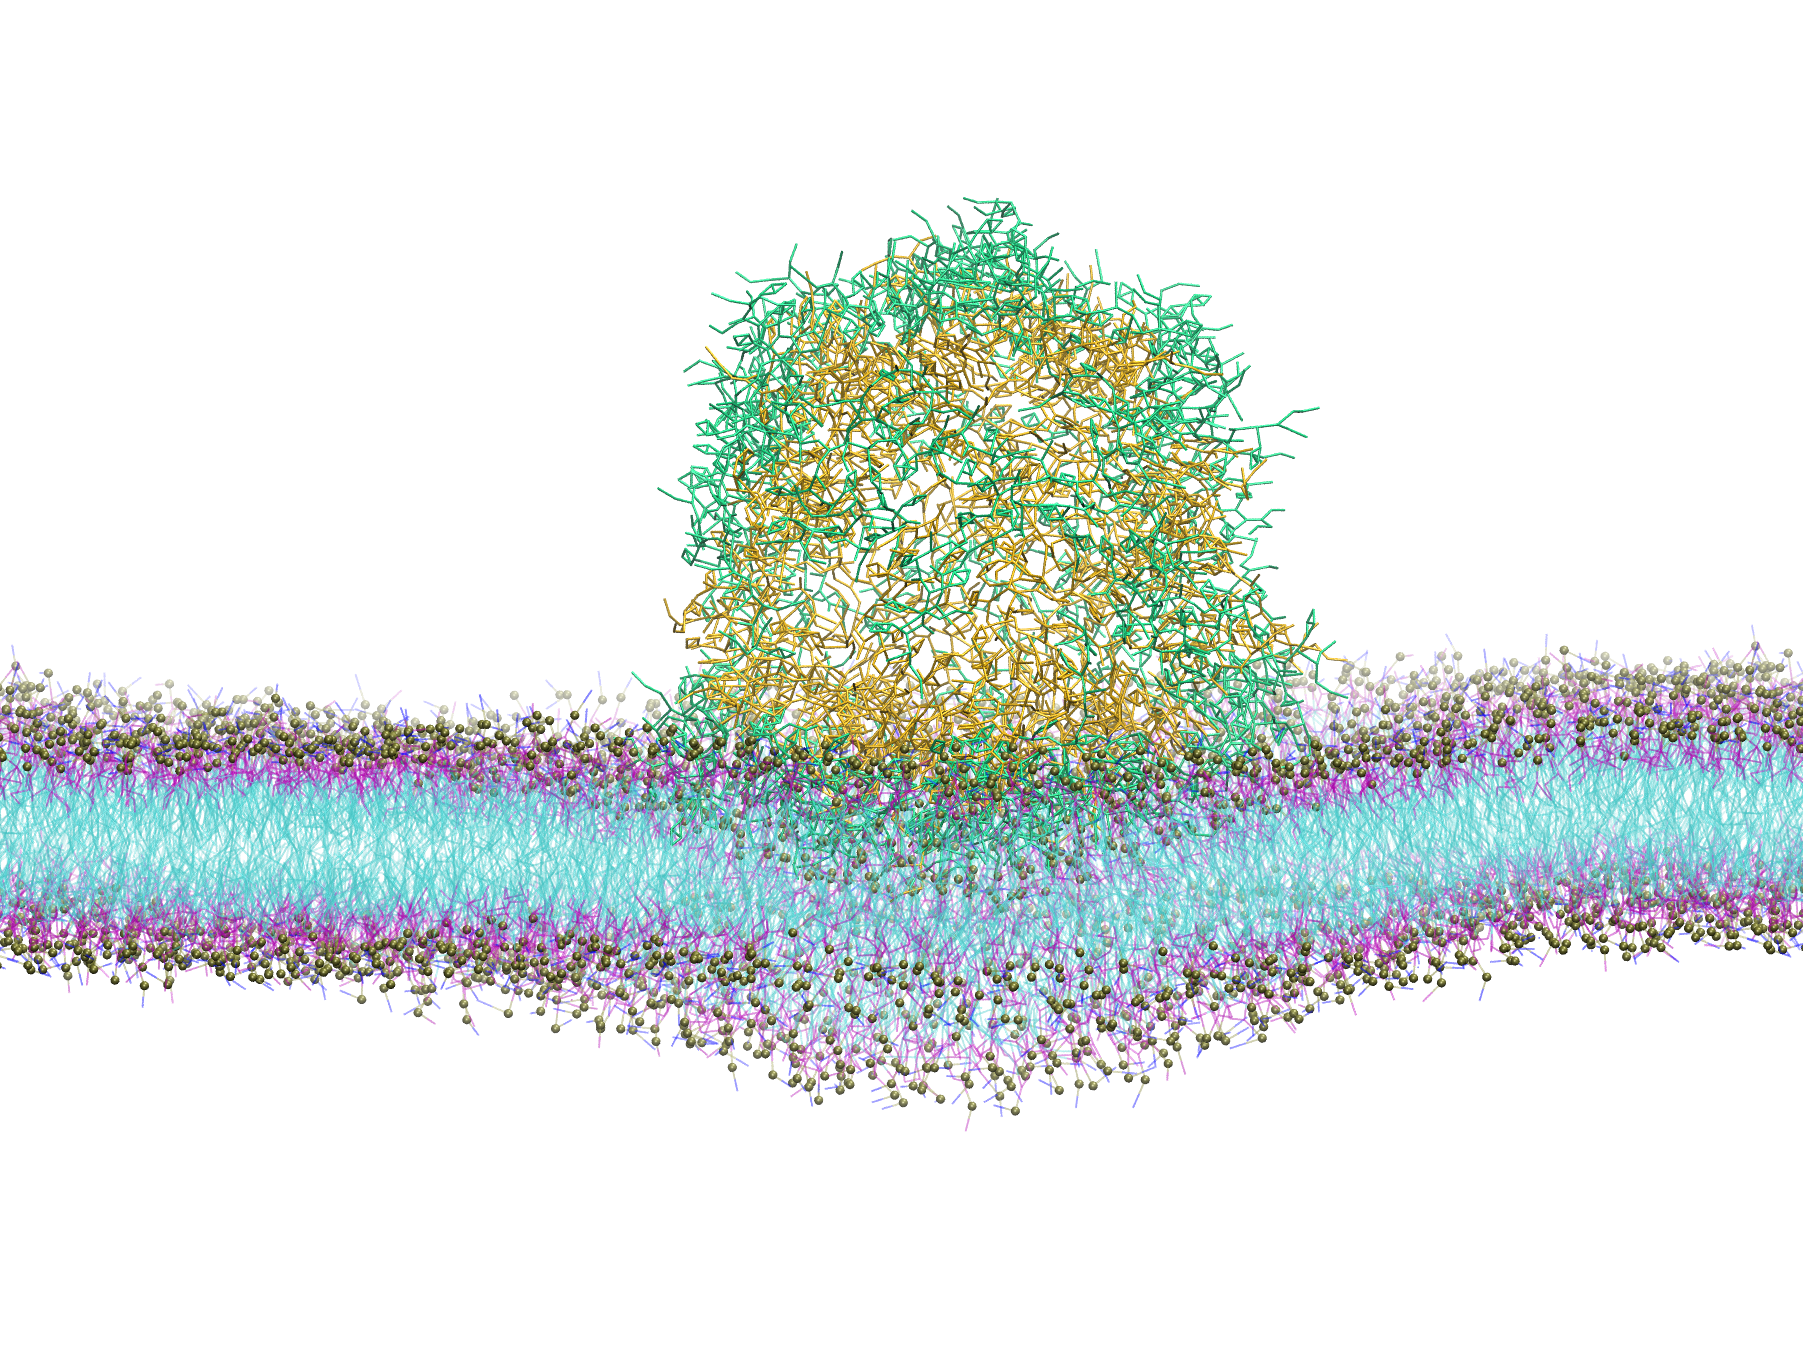
\includegraphics[width=0.45\linewidth]{3results_capsule/pics/fig7_irene.png} \label{fig:pL6_vmd_2}}
\caption[Snapshots of multiscale simulations of capzip on model membranes]{(a) Atomistic structure of a pentagonal subunit on a 740-lipid bacterial model membrane of composition DLPC/DLPG 3:1 (initial configuration). Peptide backbone in line and cartoon representation; lipids in cyan lines (DLPC) and blue ones (DLPC), all lipids phosphate in golden van der Waals beads. (b) coarse-grained (MARTINI) representation of the buckyball bilayer on a 2880 lipids bacterial model membrane (final configuration of the trajectory). Protein in bonds representation: green outer buckyball layer, yellow inner one. Lipids in line representation, coloured by bead type, and lipids phosphate in golden van der Waals beads. [VMD software \citet{HUMP96}]}
\label{fig:pL6_vmd}
\end{figure}


\section{Simulations details} \label{sec:details}

All simulations were performed with the GROMACS software, version 5.5 and 2016 \citep{Berendsen1995,Abraham2015,gromacs_man}. 

\subsection{Atomistic simulations}
\paragraph{Simulations in solution} The atomistic coordinates for the peptidic supramolecular assemblies described in Section \ref{sec:build} (Figure \ref{fig:BTI_vmd}, E) were built combining GROMACS tools and the MOE software \citep{moe}.
%
Simulations were run with the GROMOS 53A6 force field \citep{Oostenbrink2004}. Parameters for the central residue connected with the peptidic chains were computed with the ATB server \citep{Malde2011, Koziara2014}; the ones for the bonds joining this residue to the antimicrobial side chains were derived from the values tabulated in the force field for analogous ones.
%
A python module has been designed to manipulate GROMACS topology objects for the GROMOS force field and add peptide bonds at the location required (see Appendix \ref{sec:Appendix_software} for details). This is useful for multibranched peptides which are not supported by the standard GROMACS tools, and for which a manual implementation would be otherwise needed.

The systems were solvated with single point charge (SPC) water \citep{Berendsen1981} and counter ions were added (Na$^+$ or Cl$^-$); further ions were introduced to reach the concentration of 150 mM, to reproduce the experimental conditions.
%
For simulations of a single $\beta$-sheets, or of the pentagonal subunit in solution, the systems were energy minimised with a steepest descent algorithm, then equilibrated in the NVT ensemble with decreasing positional restraints at increasing temperatures (100 K, 200 K, 250 K, 300 K and respectively 1000, 1000, 500, 250 kJ/mol$\cdot$nm$^2$ restraints, 100 ps each); then in the NPT ensemble, without restraints, at the same temperatures steps and for the same time. Production followed for 100 ns.

For the buckyball bilayer structure the above equilibration was insufficient. Due to the construction procedure, two thirds of the arms are not properly paired along the edges, and with a short equilibration they drift away from each other within a few nanoseconds.
%
Therefore, after an NVT equilibration as above, strong flat-bottom restrains (1000 kJ/mol$\cdot$nm$^2$) were placed between the center of mass of imperfectly aligned arms throughout the NPT heating, to penalise their mutual separation with respect to their initial distance (100 ps runs at 100 K, 200 K and 250 K and 35 ns at 300 K).
%
This was followed by a series of 10 ns runs at 300 K with decreasing flat-bottom restraints (750, 500 and 250 kJ/mol$\cdot$nm$^2$) and by a free production run (100 ns).
%
Three different replicas were run, generated from the final configuration of the 300 K NPT run with 1000 kJ/mol$\cdot$nm$^2$ restraints.

Throughout all the simulations, the temperature was maintained by independently coupling the protein and the solvent (plus ions) to two external temperature baths using a velocity rescale thermostat \citep{Bussi2007} with coupling constant $\tau _T$ of 0.1 ps. The pressure was kept at 1 bar by Berendsen \citep{Berendsen1984} or Parrinello-Rahman barostat \citep{Parrinello1981} (for the equilibration phases and the production run respectively) using an isotropic coupling, with isothermal compressibility of 4.5 $\times$ 10$^{-5}$ bar$^{-1}$ and coupling constant $\tau_P$ of 1 ps. Electrostatic interactions were treated using the smooth Particle Mesh Ewald (PME) algorithm \citep{Essmann1995} with a Fourier grid spacing of 0.12 nm, and a short-range cutoff of 0.9 nm. The van der Waals interactions were treated with a plain 0.9 nm cutoff. All atomistic runs were performed using a 2 fs time step. An overview of the simulations of peptide assemblies in solution is given in Table \ref{table:sim_all}.

\paragraph{Simulation with membranes} The atomistic coordinates for the bacterial membrane bilayer were built with the PACKMOL software \citep{Martinez2009}, from pdb files of a single DLPC \citep{PogerOrig} and DLPG \citep{Kukol2009} molecule. Two bilayers were built, made respectively of 512 and 740 lipids, with composition DLPC/DLPG (3:1). The initial area per lipid was set to 0.70 nm$^2$, above the values found experimentally for either lipid species (0.608(12) nm$^2$ for DLPC \citep{Kucerka2011} and 0.656(12) nm$^2$ for DLPG \citep{Pan2012}). An area per lipid compatible (equal within the error) with the experimental values was reached during a 400 ns equilibration (see details below), the final configuration of which was used for simulations with the peptide.
% VERIFY WE CAN RUN IT!!!
Given the analysis performed on the bacterial bilayer (see Section \ref{sec:lip_atom_bact}), for DLPC we opted for simulating a large membrane only. Accordingly, we produced a bilayer with 748 lipids and initial area per lipid of 0.68 nm$^2$.

For membrane-peptide atomistic simulations, the initial configuration was generated from the equilibrated bilayer and the equilibrated pentagonal subunit (after 100 ns run with positional restraints on the C$^\alpha$), placing the subunit plane parallel to the membrane and close to it (Figure \ref{fig:pL6_vmd_1}).
%
The inflategro script \citep{Kandt2007} was used to solve the partial overlap of peptide side chains with lipid molecules, removing the overlapping lipids if necessary.
%In the configuration chosen, 6 and 3 lipids are removed from the 512 and 740 lipids bacteria membrane patch respectively and 13 from the 748 mammalian membrane one.
%
The two bilayers fit the pentagonal subunit with respectively 3.5 nm and 5.4 nm distance between its periodic boundary images (along both $x$ and $y$).

For simulations involving membranes, the version 54A7 of the GROMOS force field \citep{Schmid2011} was initially chosen and it is thus used for simulations of the 512-lipid bilayers, but, upon further research, version 54A8 \citep{Oostenbrink2005, Reif2013} was deemed more suitable and thus selected for the runs on the larger membranes. Lipid parameters were taken from \citep{PogerOrig} for DLPC, while for DLPG they were built from the ones available in the literature for POPG \citep{Kukol2009}.

The simulations set-up is as above, except for the use of three thermal coupling groups (peptide, membrane, water plus ions), a semi-isotropic pressure coupling, and a larger cut off radius for both Coulomb and van der Waals interactions (1.2 nm). Additionally, for the 512-lipid membrane, a Reaction Field \citep{Tironi1995} was used instead of PME long range electrostatic treatment (with cut off radius 1.4 nm), inherited from the setup of the simulations used for lipids parametrisation. This was changed to PME when simulating the larger membrane, to be more consistent with the protein parametrisation. Control simulations on membrane bilayers without peptide showed that the results in terms of area per lipid are compatible with the ones obtained using PME.

Each membrane bilayer was first equilibrated for 50 ps in NPT conditions at 50 K, then the temperature was gradually increased up to 300 K in 500 ps, and finally a 400 ns production was run. A similar equilibration procedure was followed for peptide-membrane systems.

Additional simulations were performed applying an external electric field to the membrane, pointing from the side hosting the peptide to the opposite one, to mimic the membrane potential and verify how the peptide affects the response to external stimuli.
%
In a first run the field was increased by 20 mV/nm steps every 200 ns (or 10 mV/ns when reaching the critical value), until poration was induced (at 130 mV/nm).
%
Another simulation was performed for both the 512 and 740-lipid bilayers with the peptide, with the threshold field of 130 mV/nm, starting from the unperturbed membrane configuration (three replicas each).
%
As a control, analogous test simulations were run on the 512-lipid bacterial bilayer without the peptide, assessing the electroporation threshold at the higher value of 140 mV/nm.

To be noticed that the field across the bacterial inner membrane can be estimated to be around 35 mV/nm, and across the mammalian one around 20 mV/nm (an estimate computed from, respectively, a -130/-150 mV and -70/-90 mV potential \citep{Yeaman2003,Wilson2011} and an estimate membrane thickness of 4 nm). However, previous computational work often explored the effects of higher fields, up to 500 mV/nm \citep{Tieleman2004, Bockmann2008, Piggot2011}, to witness poration within the simulations time, according to the resources available.

An overview of the simulations of peptide-membrane systems is given as well in Figure \ref{table:sim_all} (control simulations on pure membrane are listed in SI Table \ref{table:SI_membrane}).

\subsection{SIRAH coarse-grained simulations}
SIRAH coarse-grained simulations were run with the SIRAH force field, version 2.0 \citep{Machado2018}. Peptide coordinates for the buckyball geometry were obtained from the atomistic ones using the converter distributed with force field, with a customised mapping for the central residue. Parameters for the central residue were built from comparison with similar chemical moieties. All simulations were run adding Cl$^-$ counter ions to balance the positive charges of the peptide and additional Na$^+$  and Cl$^-$ ones to reach a 150 mM concentration.

While for simulations of the peptide buckyball in solution our multiscale procedure includes SIRAH, for simulations on membranes we focussed on atomistic and MARTINI simulations only. This has been performed in the interest of time, and due to technical difficulties in preliminary SIRAH runs with membranes (in particular in tuning the pressure coupling).
%
This is likely due to a suboptimal equilibration procedure; indeed, there are few benchmarks on SIRAH for lipids so far \citep{Barrera2019}, and none for systems as large as the one studied here.

For SIRAH simulations, the temperature coupling was performed with a velocity rescale thermostat \citep{Bussi2007} and coupling constant $\tau _T$ of 0.1 ps, and the pressure coupling at 1 bar pressure, with 4.5 $\times$ 10$^{-5}$ bar$^{-1}$ isothermal compressibility, using a Parrinello-Rahman barostat \citep{Parrinello1981} with a $\tau _P$ of 6 ps. Electrostatic interactions were treated using the PME algorithm \citep{Essmann1995}, with a short-range cutoff of 1.2 nm and relative dielectric constant of 1. The van der Waals interactions are treated with a 1.2 nm cutoff and no long range corrections.

After energy minimization, a 4 ns NVT equilibration was run at 300 K, followed by a 10 ns NPT run, both with positional restraints (1000 kJ/mol$\cdot$nm$^2$) on the solute. Two 10 ns run (NPT ensemble, 300 K) were then performed with backbone restraints of 1000 and 100 kJ/mol$\cdot$nm$^2$, respectively. Similar to the procedure adopted for atomistic simulations, flat bottom positional restraints (1000 kJ/mol$\cdot$nm$^2$) were enforced on the unpaired arms during the latter. After this, three additional 10 ns equilibrations were run at 300 K, with no backbone restraints and decreasing flat bottom ones (respectively 750, 500 and 250 kJ/mol$\cdot$nm$^2$). Finally the production run was carried on for 1 $\mu$s. All runs were performed with a 20 fs time step.

\subsection{MARTINI coarse-grained simulations} \label{sec:MARTINI_sim_det}
For MARTINI \citep{Marrink2007, Monticelli2008} coarse-grained simulations, peptide coordinates were obtained from the atomistic ones using martinize.py \citep{DeJong2013} with a customised mapping for the central residue. Parameters were obtained with the same script for the arms, while pycgtool.py \citep{Graham2017} was used for the central residue. Parameters for the joining bonds were derived from tabulated values of analogous ones.

Initial coordinates for the self-assembly simulations were obtained with GROMACS tools, placing the desired amount of coarse-grained molecules in the simulation box with random positions.
%
The side of the cubic box was chosen as 44 nm, and three different peptide concentrations were simulated: 1.25 mM (60 molecules), 2.50 mM (120 molecules) and 10 mM (480 molecules), all for 10 $\mu$s.

The bacterial and mammalian model membranes, hosting 2880 lipids each, were built with insane.py \citep{Wassenaar2015}, with composition DLPC/DLPG (3:1) and pure DLPC respectively. The simulations parameters used for lipids are consistent with \citet{SiewertJ.Marrink2003}. The peptide-membrane systems were built placing the buckyball at a minimum distance of 1 nm from the membrane surface.

For all standard MARTINI simulations, counter ions only were added, while for the ones run with Polar MARTINI, additional Na$^+$ and Cl$^-$ were inserted to reach a 150 mM concentration.

For simulations with the standard water model, the temperature coupling was performed with a velocity rescale thermostat \citep{Bussi2007} with a coupling constant $\tau _T$ of 1 ps. An isotropic or semi-isotropic pressure coupling was applied (simulations of peptide in solution and peptide on membrane respectively) at 1 bar pressure, with 4.6 $\times$ 10$^{-5}$ bar$^{-1}$ isothermal compressibility, using a Berendsen \citep{Berendsen1984} or Parrinello-Rahman barostat \citep{Parrinello1981} (equilibration and production phase respectively) with $\tau _P$ of 2 ps or 12 ps.
%
Coulomb interactions were treated with a Reaction Field scheme \citep{Tironi1995} and cut off radius of 1.1 nm, van der Waals interactions with a cut off scheme and the same cut off radius. The relative dielectric constant is set to 15.
%
Simulations performed with the polar water model were run with the parameters above, except the relative dielectric constant set to 2.5, and the choice of a PME scheme for the long range Coulomb interaction (1.2 nm cut off radius).
The choice of the respective dielectric constant and electrostatic treatment is in agreement with the optimal setup found in the parametrisation publications of the respective water models.

For simulations of the capsule in solution, for both water models, after energy minimization, four 10 ns equilibration runs (NPT ensemble, 300 K, 10 fs time step) were performed with flat bottom positional restraints on the unpaired arms (respectively at 1000, 750, 500 and 250 kJ/mol$\cdot$nm$^2$) - as done for the other force fields.
%
Finally the production run was carried on for 1 $\mu$s. All runs were performed with a 20 fs time step.

It is interesting to notice that the MARTINI force field with the standard water model produced very similar results with or without such refined equilibration procedure, as confirmed by simulations of the buckyball run after a short unrestrained equilibration only (500 ps, 1 fs timestep). However, we choose to follow the same procedure as for the other force fields to have more consistent results, and be certain that the differences observed are due only to the parametrisation an not to the equilibration procedure.

From the final configurations of two out of the three standard MARTINI replicas, atomistic coordinates were obtained using the MARTINI backward tool (version 5) \citep{Wassenaar2014} and run for additional 200 ns with the set up used for atomistic simulations.

The equilibration for the self-assembly simulations (run only with the standard MARTINI model) included only an energy minimization, followed by a 1 ns equilibration with the Berendsen barostat, before switching to Parrinello-Rahman for the 10 $\mu$s production.

The membranes used in MARTINI simulations are equilibrated for 1 $\mu$s with standard water and the final configuration is used to build the peptide-membrane systems, together with the capsule structure (obtained after the equilibration runs). The full system is energy minimised, equilibrated for 500 ps and production is followed for 10 $\mu$s for simulations with the standard water, and 500 ns with polar water (due to the faster binding and the speed up granted by the electric field).

The adoption of polar water allows to perform electroporation experiments also with the MARTINI force field (while the standard water, not bearing a dipole, is unable to screen the externally applied electric field, resulting in unphysical effects).
%
We thus resorted to a procedure similar to the one employed for atomistic simulations, testing an external electric field of magnitude 20 mV/nm and 40 mV/nm, without proceeding further as the latter gave poration in presence of the peptide.
%
It is possible that longer simulations would allow to observe this behaviour even with lower values of the force field, however, in the interest of time, we selected these two for further investigation.

We selected a configuration from the early stages of poration (at 40 mV/nm), where the pore showed a diameter of 2 nm, and prolonged the simulation switching to isotropic pressure coupling. This allows the pore to expand in a controlled manner. Indeed, in a semi-isotropic pressure coupling scenario, the pressure in the $z$ direction suddenly decreases when a pore forms, as water can pass through the membrane. This is also the direction of the applied electric field. The barostat algorithm reacts decreasing the $z$ side of the box, in an effort to restore the target pressure in this direction, but to accommodate all the molecules the box must necessarily expand in the $x$ and $y$ directions in an excessive way.

Control simulations with the two values of the electric field mentioned were performed on the membrane alone. The same procedure, i.e.\ simulations with capsule and electric field plus control simulations on the membrane only was applied to the pure DLPC membrane as well (except for the additional simulation after poration, as this is not observed for the DLPC membrane).


\begin{figure}[p!]
\centering
%\small
\scriptsize
 \def\arraystretch{1.6}
\begin{tabular}{llccccc}
\multicolumn{7}{c}{\small\textbf{Table of simulations of capzip assemblies}} \\
 \hline
Peptides & Lipids & Box (nm) & C (mM) & E (mV/nm) & Time (ns) & Rep. \\
 \hline
\multicolumn{7}{c}{\textbf{United atom GROMOS (GR)}} \\
 $\beta$-sheet & -- & 4 & 0 & -- & 20 & 16$^a$ \\
 PS (10) & -- & 12 & 0 & -- & 100 & 1$^a$ \\
 BB (120) & -- & 22 & 150 & -- & 100 & 3$^a$ \\
 BB-back (120) & -- & 22 & 150 & -- & 200 & 2$^a$ \\
 PS (10) & 512 (b) & 12 & 150 & -- & 500 & 2$^b$ \\
 PS (10) & 740 (b) & 14 & 150 & -- & 500 & 1$^c$ \\
 PS (10) & 740 (m) & 14 & 150 & -- & 500 & 1$^c$ \\
 PS (10) & 512 (b) & 12 & 150 & 130 & 75$^P$, 20$^P$, 71$^P$ & 3$^b$ \\
 PS (10) & 740 (b) & 14 & 150 & 130 & 60$^P$, 50$^P$, 70$^P$ & 3$^c$ \\
 PS (10) & 740 (m) & 14 & 150 & 130 & 20$^P$, 28$^P$, 39$^P$ & 3$^c$ \\
 \hline
\multicolumn{7}{c}{\textbf{Coarse-grained SIRAH (SI)}} \\
 BB (120) & -- & 22 & 150 & -- & 1000 & 3 \\
 BM (60) & -- & 22 & 150 & -- & 1000 & 2 \\
 \hline
\multicolumn{7}{c}{\textbf{Coarse-grained Polar MARTINI (MA\_P)}} \\
 BB (120) & -- & 22 & 150 & -- & 1000 & 2 \\
 BM (60) & -- & 22 & 150 & -- & 1000 & 2 \\
 BB (120) & 2880 (b) & 30 & 150 & -- & 10000 & 1 \\
 BB (120) & 2880 (b) & 30 & 150 & 20 & 500 & 1 \\
 BB (120) & 2880 (b) & 30 & 150 & 40 & 168$^P$ & 1 \\
 BB (120) & 2880 (m) & 30 & 150 & -- & 10000 & 1 \\
 BB (120) & 2888 (m) & 30 & 150 & 20 & 500 & 1 \\
 BB (120) & 2888 (m) & 30 & 150 & 40 & 500 & 1 \\
 \hline
\multicolumn{7}{c}{\textbf{Coarse-grained MARTINI (MA)}} \\
 BB (120) & -- & 22 & 150 & -- & 1000 & 3 \\
 BM (60) & -- & 22 & 150 & -- & 1000 & 1 \\
 Random (60) & -- & 22 & 0 & -- & 10000 & 1 \\
 Random (120) & -- & 22 & 0 & -- & 10000 & 1 \\
 Random (480) & -- & 22 & 0 & -- & 10000 & 1 \\
 BB (120) & 2880 (b) & 30 & 0 & -- & 10000 & 2 \\
 BB (120) & 2880 (m) & 30 & 0 & -- & 10000 & 1 \\
 \hline
 \end{tabular}
 \begin{tabular}{lcccccc}
 \hline
 \hline
\end{tabular}
\vspace{0.5cm}
\captionof{table}[Simulations of capzip assemblies, in water and on membranes]{Table of simulations of capzip assembly in water and on membranes.
%
Peptides: PS - pentagonal subunit; BB - buckyball bilayer; BB-back - buckyball bilayer backmapped; BM - buckyball monolayer; Random - random initial configuration. In parenthesis, the number of capzip molecules.
%
Lipids: number of lipids and model, with (b) - bacterial model (DLPC/DLPG 3:1), (m) - mammalian model (DLPC).
%
Rep: number of replicas.
%
Force field indicated in bold headers: GR - united atom GROMOS ($^a$ version 53A6 \citep{Oostenbrink2004}, $^b$ 54a7 \citep{Schmid2011}, $^c$ 54a8 \citep{Reif2012}), SI - coarse-grained SIRAH \citep{Machado2018}, MA - coarse-grained MARTINI \citep{Marrink2007, Monticelli2008}, MA\_P - coarse-grained MARTINI with polar water \citep{Yesylevskyy2010}.
%
Superscript P in the time length denotes observation of poration.
%
For electroporation simulations on pure membranes, see Supplementary Table \ref{table:SI_membrane}.}
\label{table:sim_all}
\end{figure}

\section{Analysis} \label{sec:analysis}

All the analysis was performed combining tools from GROMACS \citep{Berendsen1995,Abraham2015,gromacs_man}, MDAnalysis \citep{Michaud-Agrawal2011,Gowers2016} and packages developed for the purpose (see \ref{sec:Appendix_software}).

In Section \ref{sec:build} we presented an evaluation of the occurrence of $\pi$-stacking between Tryptophan residues in the $\beta$-sheet simulations. The computation was performed as follow: for each pair of Trp residues, we computed the minimum distance between the centre of mass of their side chains benzene rings (in function of time), as well as the angle formed by their two planes. We consider as candidates for an aromatic interaction rings which were between 0.45 and 0.7 nm of distance, accordingly to the classical definition \citep{Burley1986} and what found generally in crystal structures \citep{Anjana2012}. 
%
Then, we defined a parallel $\pi$-stacking if the angle between the ring was smaller than 45$^{\circ}$, and a T-shaped (perpendicular) one if the angle fell between 80$^{\circ}$ and 100$^{\circ}$ (as observed in the majority of T-shaped stacking in crystal structures) \citep{Anjana2012}. Occupancy was found normalising the number of frames in which the interaction appeared by the number of frames considered for the analysis (2000 $\times$ 16, 1 ever 100 ps).    

For the $\beta$-sheet simulations and whenever in the following we mention hydrogen bond computations, this was performed using the default set up of GROMACS. With such setup, a donor atom (with a polar hydrogen bonded to it) and an acceptor one are classified as interacting through hydrogen bond if the donor-acceptor distance is smaller than 0.35 nm and the hydrogen-donor-acceptor angle is smaller than 30$^{\circ}$.
    
\subsection{Simulations in solution}
Several analysis on the structure and chemico-physical properties of the simulated buckyball bilayer in solution were performed.

\begin{itemize}
\item The Radius of gyration ($R_g$), and Root Mean Square Deviation with respect to the initial configuration (RMSD) were computed (GROMACS).

\item To get the average distribution of the mass of the capsule around its center, the Radial Distribution Function (RDF) of protein masses around their center of mass was computed (GROMACS), considering only the second half of the trajectory. The profile was fitted with a Gaussian function (R software \citep{R}): the position of its maximum can be taken as the average radius of the capsule, and its Full Width at Half Maximum (FWHM) as an estimate of the capsule wall thickness.

\item The dynamical character of the structure was assessed computing the correlation of motion between molecules (GROMACS). The central atom (or bead) from which the arms depart was taken as reference. For all the pairs ($i, \, j$) of such reference positions, the covariance of motion was computed along each direction. The total covariance was obtained as: $\sigma^2(i,j) = \sigma_x^2(i,j) + \sigma_y^2(i,j) + \sigma_z^2(i,j)$. Finally the measure was normalised to obtain the correlation:
\begin{equation}
corr(i,j) = \frac{\sigma^2(i,j)}{\sqrt{\sigma^2(i,i)\,\cdot\,\sigma^2(j,j)}}.
\end{equation}

\item The pairing of the arms was quantified as follow. Two arms are defined as paired if their center of mass is closer than a cut off distance of 1.2 nm (GROMACS and R postprocessing). This simple measure discards more precise information on the orientation of the chains with respect to each other, and aims at checking whether the network of molecules present in an ideal buckyball structure is maintained. In the ideal buckyball, contacts within the same layer sum up to 90 for each layer (and so 180 in a bilayer). This measure can be easily applied to any description (atomistic or coarse-grained) without disagreement in the interpretation. Given the loose character of the measure, we considered only the pairings surviving more than 90\% of the simulation time.

\item To characterise the chemical determinants that promote the assembly, we investigated the interactions between amino acids of different types, computing the number of contacts between backbone and side chains of single amino acids (function implemented in MDAnalysis, see Appendix \ref{sec:Appendix_software}). We filtered for the ones present at least 50\% of the simulation time, and remove the ones between residues in the same arm, finally we classified them by amino acid type.
%
Backbone contacts are computed considering C$^\alpha$s of residues (or the corresponding coarse-grained bead); side chains ones using selected reference atoms/beads (respectively for GROMOS, SIRAH and MARTINI: CZ/BCZ/SC2 for Arg, CZ2/BNE/SC4 for Trp, OG1/BPG/SC1 for Thr and CD/BCD/SC1 for Glu); finally mixed ones if the proximity is between a C$^\alpha$ and the side chain reference position. The distance threshold is set to 0.6 nm.

\item For atomistic simulations, the inter molecular hydrogen bonds between amino acids have been computed (as explained previously with GROMACS) and grouped by amino acid type, and by region of occurrence (e.g.\ between two backbones, side chains or connecting a backbone atom and a side chain one).

\item The Solvent Accessible Surface Area was computed for each amino acid (GROMACS). Its value was averaged in time and over all the residues at the same position in the capzip sequence. For atomistic runs, it was also normalised over the reference value for the corresponding residue type X, obtained as the theoretical measure of its SASA in a Gly-X-Gly tripeptide \citep{Tien2013}. The resulting Q$_{SASA}$ takes into account the size of the side chain, giving a measure of exposure which can be compared between different amino acids. 
%
This normalisation is however inappropriate for coarse-grained models, due to the differences between the atomistic SASA obtained in experiments and the beads employed in the simulations, so that only the absolute SASA values are given.

\item Finally, the contribution to the total energy of the system deriving from Coulomb and Lennard-Jones interactions were compute (GROMACS), breaking them into interactions between protein components and between protein and solvent.
\end{itemize}

\subsection{Simulations on a membrane}

Many properties can be extracted from a membrane simulation. We report here the ones selected for analysing the simulations including membranes and capzip, while Chapter \ref{chapter:lip_par} gives an extensive overview of more of them, reiterating and expanding the description of the ones listed below.

\begin{itemize}
\item We monitored the area per lipid (ApL), i.e.\ the average space available to each lipid on the (local) membrane plane. In the case of approximately flat membranes aligned to the $xy$ plane, this can be assessed from the product of the lateral dimensions of the simulation box divided by the number of lipids in one leaflet.
%
For highly curved membranes, as the ones obtained under the effect of a strong electric field, this measure does not reflect the true spacing between lipids. In that case the true ApL was computed through the algorithm developed by \citet{Braun2011}: this first identifies the undulating reference surface of the membrane $u(\textbf{r})$ fitting a Fourier series to a set of reference positions (one atom per lipid, presently the Phosphorus atom or the Phosphate bead for coarse-grained simulations), then it computes the true ApL based on $u(\textbf{r})$ as:
\begin{equation}
ApL = \frac{1}{N} \int_{x_{box}} \int_{y_{box}} \left[ \sqrt{1 + \left( \nabla u(\textbf{r}) \right)^2} \, \right] dx\,dy
\end{equation}
where the gradient $\nabla u(\textbf{r})$ is zero for a perfectly flat surface.

\item For atomistic simulations, the deuterium order parameters S$_{CD}$ of the acyl chains is a good measure of their relative orientation and whether the chains adopt for it a narrow range of values \citep{VanLehn2014a,Douliez1998,Piggot2017}. The orientation $\theta$ with respect to the outward leaflet normal is computed for each carbon-hydrogen bond in a given position $i$ along the chain, for each lipid in the bilayer. Their spread is evaluated according to the ensemble average:
\begin{equation}
S_{CD}(i) = \frac{1}{2} \langle 3\cos^2 \theta_i - 1 \rangle.
\end{equation}
As the GROMOS force field employs a united-atom representation, the tetrahedral positions of the hydrogens are constructed based on the neighbouring carbons’ positions.

\item Another measure of the regular packing of lipids in the $xy$ plane (parallel to the membrane surface) is given by the hexagonal order parameter S$_6$ \citep{Uppulury2015}, usually employed to quantify the transition to a gel phase. Specifically, each lipid tail chain was represented by its position on the $xy$ plane, computed as the average $x$ and $y$ position of its carbon atoms.
%
For each chain $j$ the neighbouring chains $\{n\}$ were identified as the ones within a 0.65 nm radius from $j$ (Figure \ref{fig:S6_theory}). Then S$_6$ is defined as:
\begin{equation}
S_{6,j} = \frac{1}{6} \left| \sum_{k \,\in \{n\}} e^{6i\theta_{jk}} \right|
\end{equation}
with $\theta_{jk}$ the angle between the vector connecting $j$ and $k$, and the $x$ axis (and $i$ the imaginary unit). A chain is in gel phase if it has an hexagonal order parameter larger than 0.72 \citep{Uppulury2015}.
%
\begin{figure}[t!]
\centering
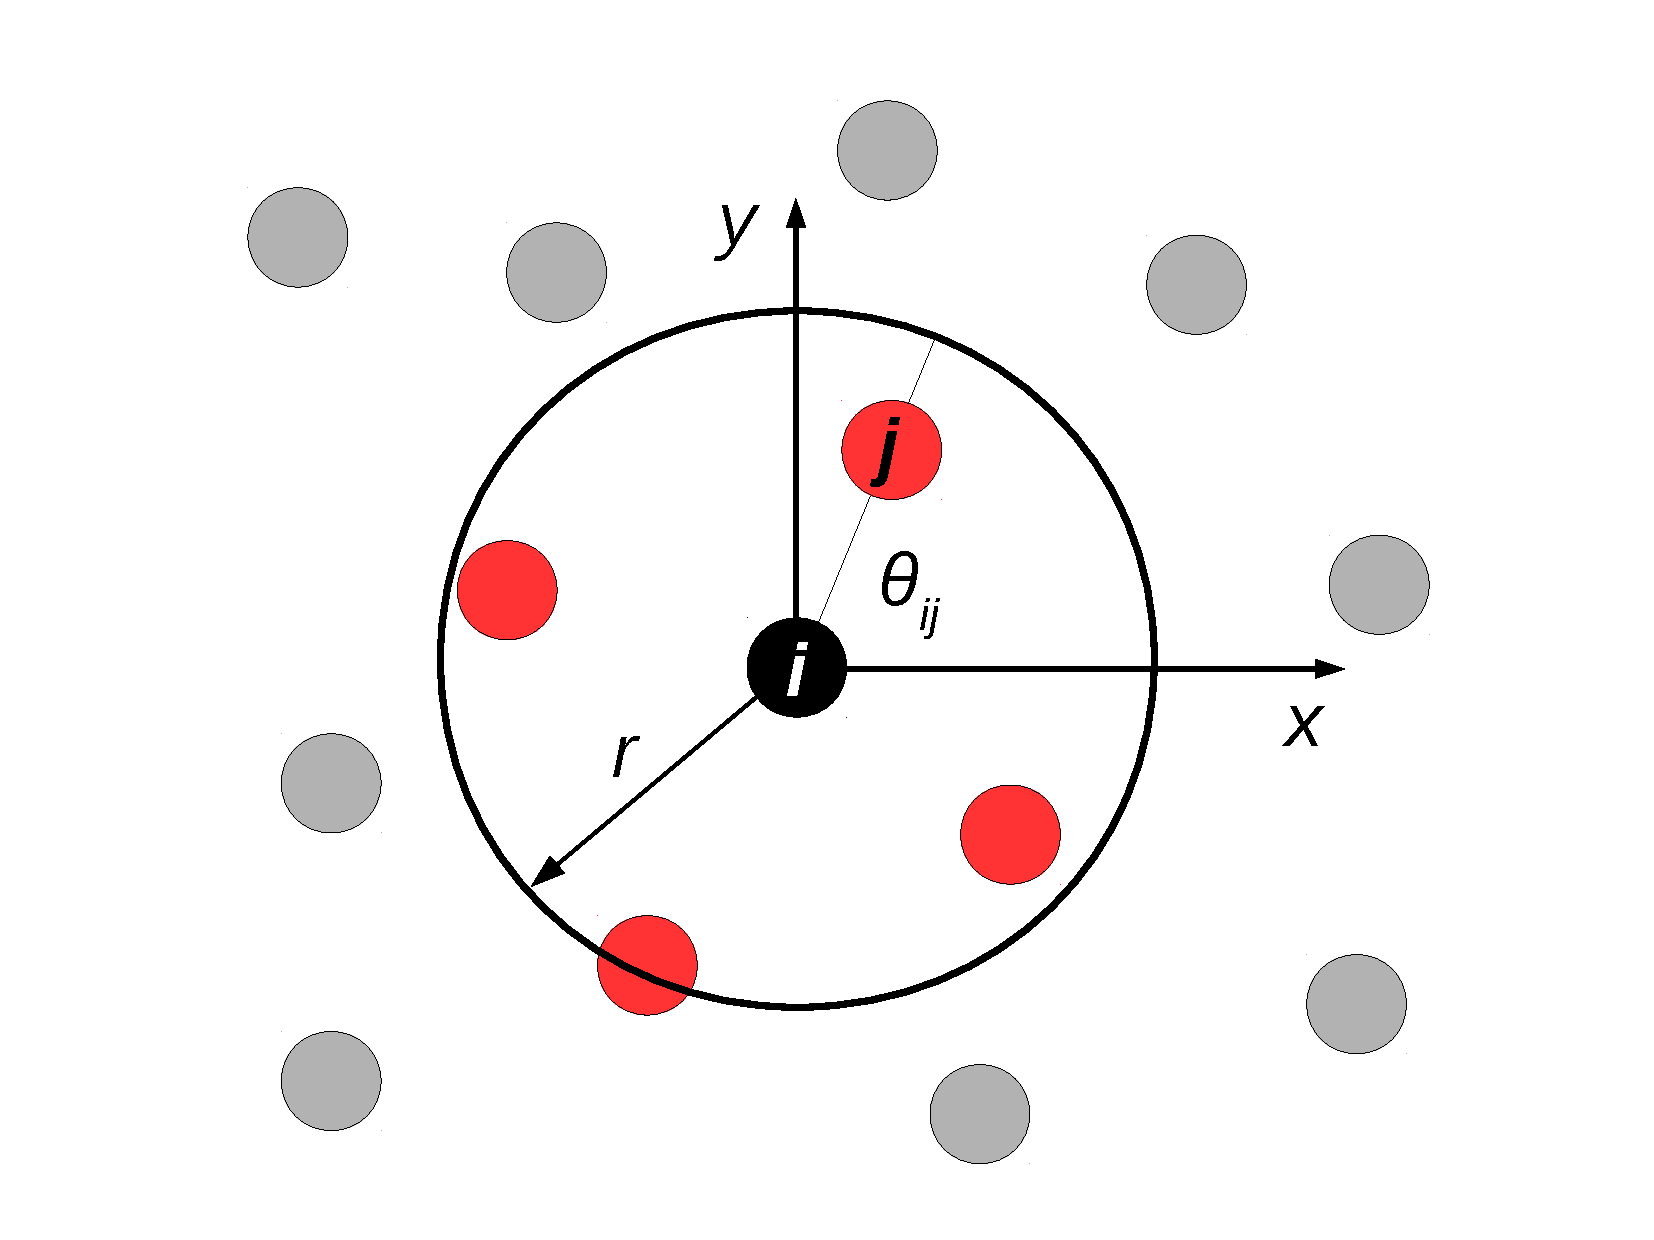
\includegraphics[width=0.55\linewidth]{3results_capsule/pics/s6_theory.pdf}
\caption[Scheme of S$_6$ computation]{Scheme of S$_6$ computation: in black the reference chain $i$, in red the chains belonging to the neighbouring chains set $\{n\}$; $r$ was chosen as 0.65 nm.} \label{fig:S6_theory}
\end{figure}

\item To evaluate the mobility of lipids on the membrane plane, for each simulation we extracted the trajectory of the phosphorus atom of every lipid, removing the jumps derived from the periodic boundary conditions treatment, to have a continuous evolution of the positions. The resulting trajectory must be centred to remove the drift of the whole system, and this can be achieved in two ways: either considering the two leaflets separately and centring each of them within the simulation box at each time frame (L$_{COM}$ procedure) or considering the bilayer as a unique object and translating its center of mass at the origin of the simulation box for each time frame (B$_{COM}$ procedure). Figure \ref{fig:com_rem_scheme} illustrates the procedures in two cases, showing how they differ if a leaflet translates with respect to the other one.

The MSD of each lipid in one leaflet was computed as a function of time: for a lipid $i$ and a given time $t$, the displacement $r_i^2(t_{start}+t)$ was computed for all $t_{start}$ such that $(t_{start}+t)$ is within the simulated time. The average over the start times and over the lipids (belonging to the same specie and leaflet) gave the MSD(t):
\begin{equation}
MSD(t) = \langle \langle r_i^2(t_{start}+t) \rangle_{start} \rangle_i.
\end{equation}
This computation was performed discarding the first part of the trajectory, the exact amount of which depends on the system, and it was chosen monitoring the area per lipid.
The diffusion coefficient D was obtained from a linear fit of the MSD(t), following Einstein equation in two dimensions \citep{Einstein1956}:
\begin{equation}
\langle r^2 \rangle = 4Dt.
\end{equation}
The fit was performed in the regions which showed a linear dependence. This implied discarding the first interval of the profile, where the behaviour is not linear, and the last one, where the poorer statistics leads to more noisy data. We choose 50 ns for both of them for atomistic simulations and 100 ns for MARTINI ones. This was done for each simulation condition of the respective resolution. As a final step, the D values from the two leaflets are averaged.

As a short hand notation, we will call the D coefficient obtained from a L$_{COM}$ removal as \emph{pure diffusion}, while the one obtained from a B$_{COM}$ removal as \emph{global diffusion}.
%
The former measures the pure random movement of a lipid with respect to its neighbours, the latter is influenced by possible collective movements of one leaflet with respect to the other.
\begin{figure}[t!]
\centering
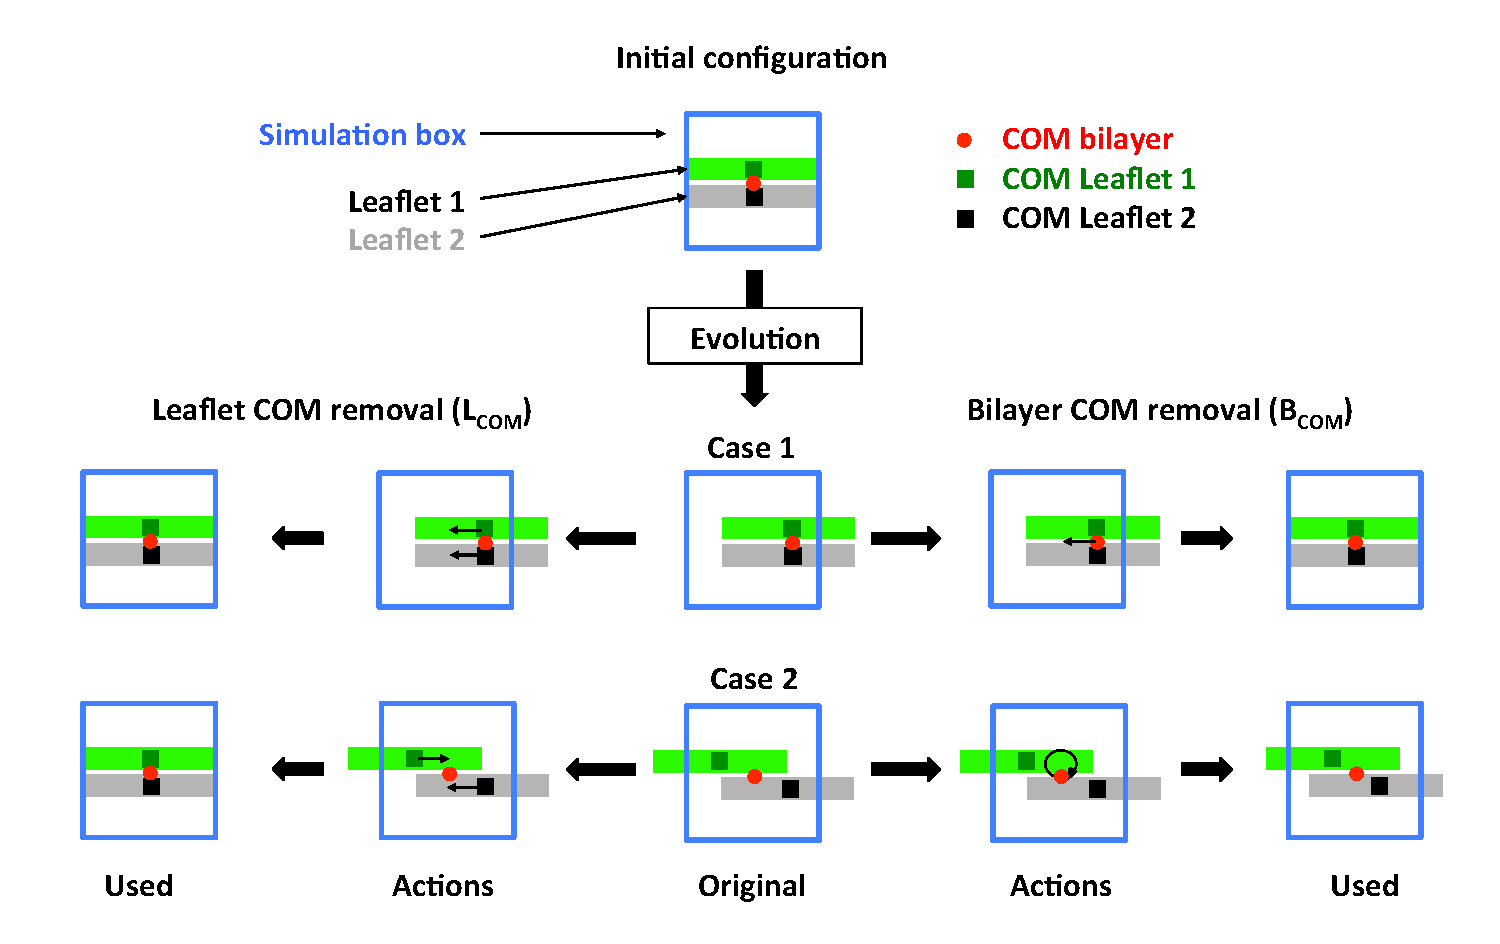
\includegraphics[width=0.95\linewidth]{3results_capsule/pics/diff_comrem} 
\caption[Scheme of trajectories preprocessing for computation of diffusion]{Scheme of two different procedures for centring a trajectory of a lipid bilayer: from the \emph{Original} configuration, coordinates are translated to remove either the bilayer or each leaflet movement. The collection of \emph{final} frames, one for each time step, gives the trajectory used to compute the MSD of lipids and thus diffusion.}
\label{fig:com_rem_scheme}
\end{figure}
\end{itemize}

For atomistic simulations of the protein on the membrane, further analysis included the following:
\begin{itemize}
\item we analysed the network of hydrogen bonds between the protein and lipids, classifying the interactions by the protein residue type and the lipid species (or lipid moiety) between which they occur. Hydrogen bonds are evaluated as described previously;
\item for selected simulations the aforementioned diffusion constant was computed selectively on the lipids which, at the initial time, were within a threshold distance from the protein or, conversely, further away from it. In this case, the trajectory was centred with respect to the peptide centre of mass, to understand how lipids move with respect to it;
\item the insertion depth of each amino acid in the membrane was calculated as the difference between the $z$ position of the lowest atom of the amino acid and the average of the maximum $z$ coordinate of the five lipids closest to it. This allows to take into account undulations of the membrane by considering the local $z$ coordinate. As for an optimally packed membrane in gel phase each lipids has 6 neighbours, the value of 5 reflects approximately the number of first neighbours in a bilayer in fluid phase.
\end{itemize}

\section{Results: capsule in solution} \label{sec:results_cap}
We list here the results for simulations of the capsule in solution: starting from the atomistic simulations, we then proceed to compare them with different coarse-grained models. However, when applicable, the plots present the results from all the parametrisations at once, anticipating the discussion of Section \ref{sec:res_multiscale}, as this makes the comparison easier. In all the plots of the section, atomistic results are color coded in violet, as opposed to yellow (SIRAH), cyan (standard MARTINI) and dark green (Polar MARTINI). Results are shown for Replica 1, unless otherwise specified. The analogous results for Replica 2 are shown in the Supplementary Material (Section \ref{sec:ch3_SI}, Figures \ref{fig:struct_UA_SIhere2}-\ref{fig:mono_bi_sasa2}). Supplementary Movies SI\_M1, SI\_M2 and SI\_M3 show GROMOS, SIRAH and Polar MARTINI runs (Replica 1); for the two coarse-grained force fields simulations of the monolayer are displayed as well (see Section \ref{sec:mono}).

\begin{figure}[t]
\centering
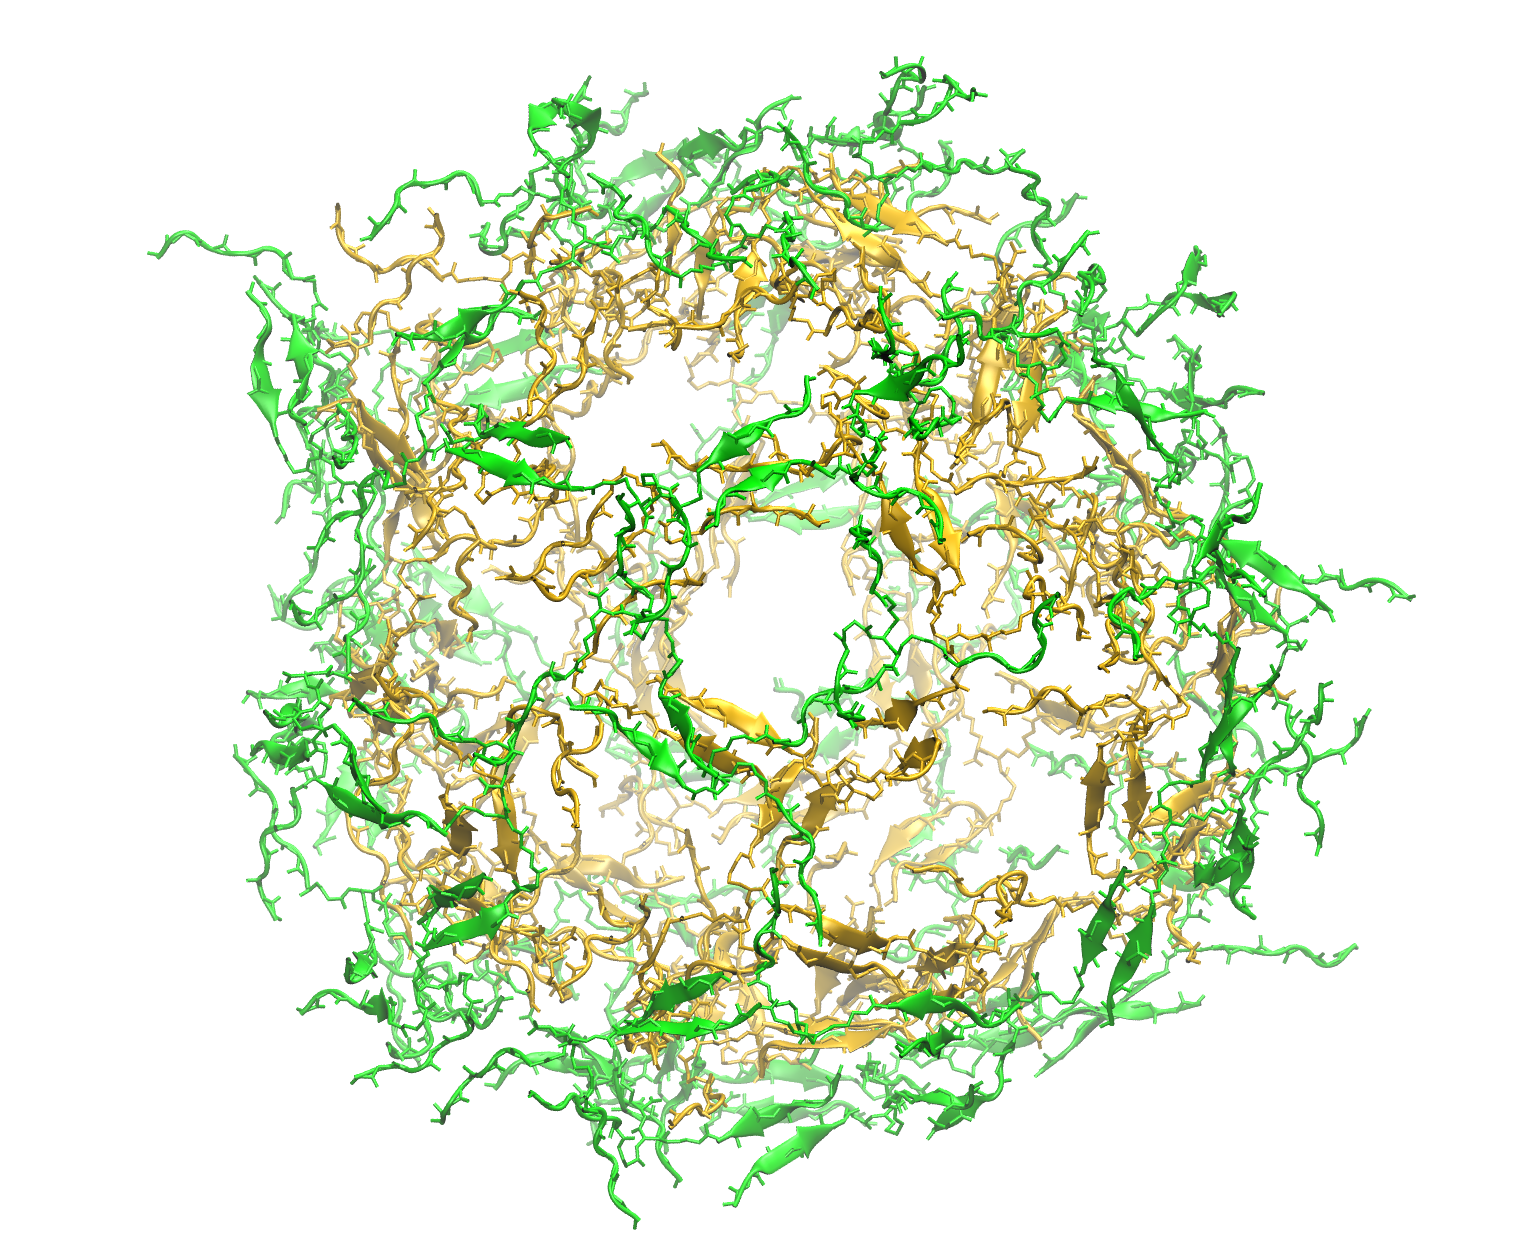
\includegraphics[width=0.5\linewidth]{3results_capsule/pics/staR3_render}
\caption[Atomistic simulations of buckyball in solution: final configuration]{Final configuration from an atomistic simulation of a buckyball in solution (100 ns, Replica 1): bonds and cartoon representation, backbone only, green external layer and yellow internal one. [VMD software \citet{HUMP96}]}
\label{fig:BTI_snap}
\end{figure}

\subsection{Atomistic simulations}

\begin{figure}[p!]
\centering
\subbottom[]{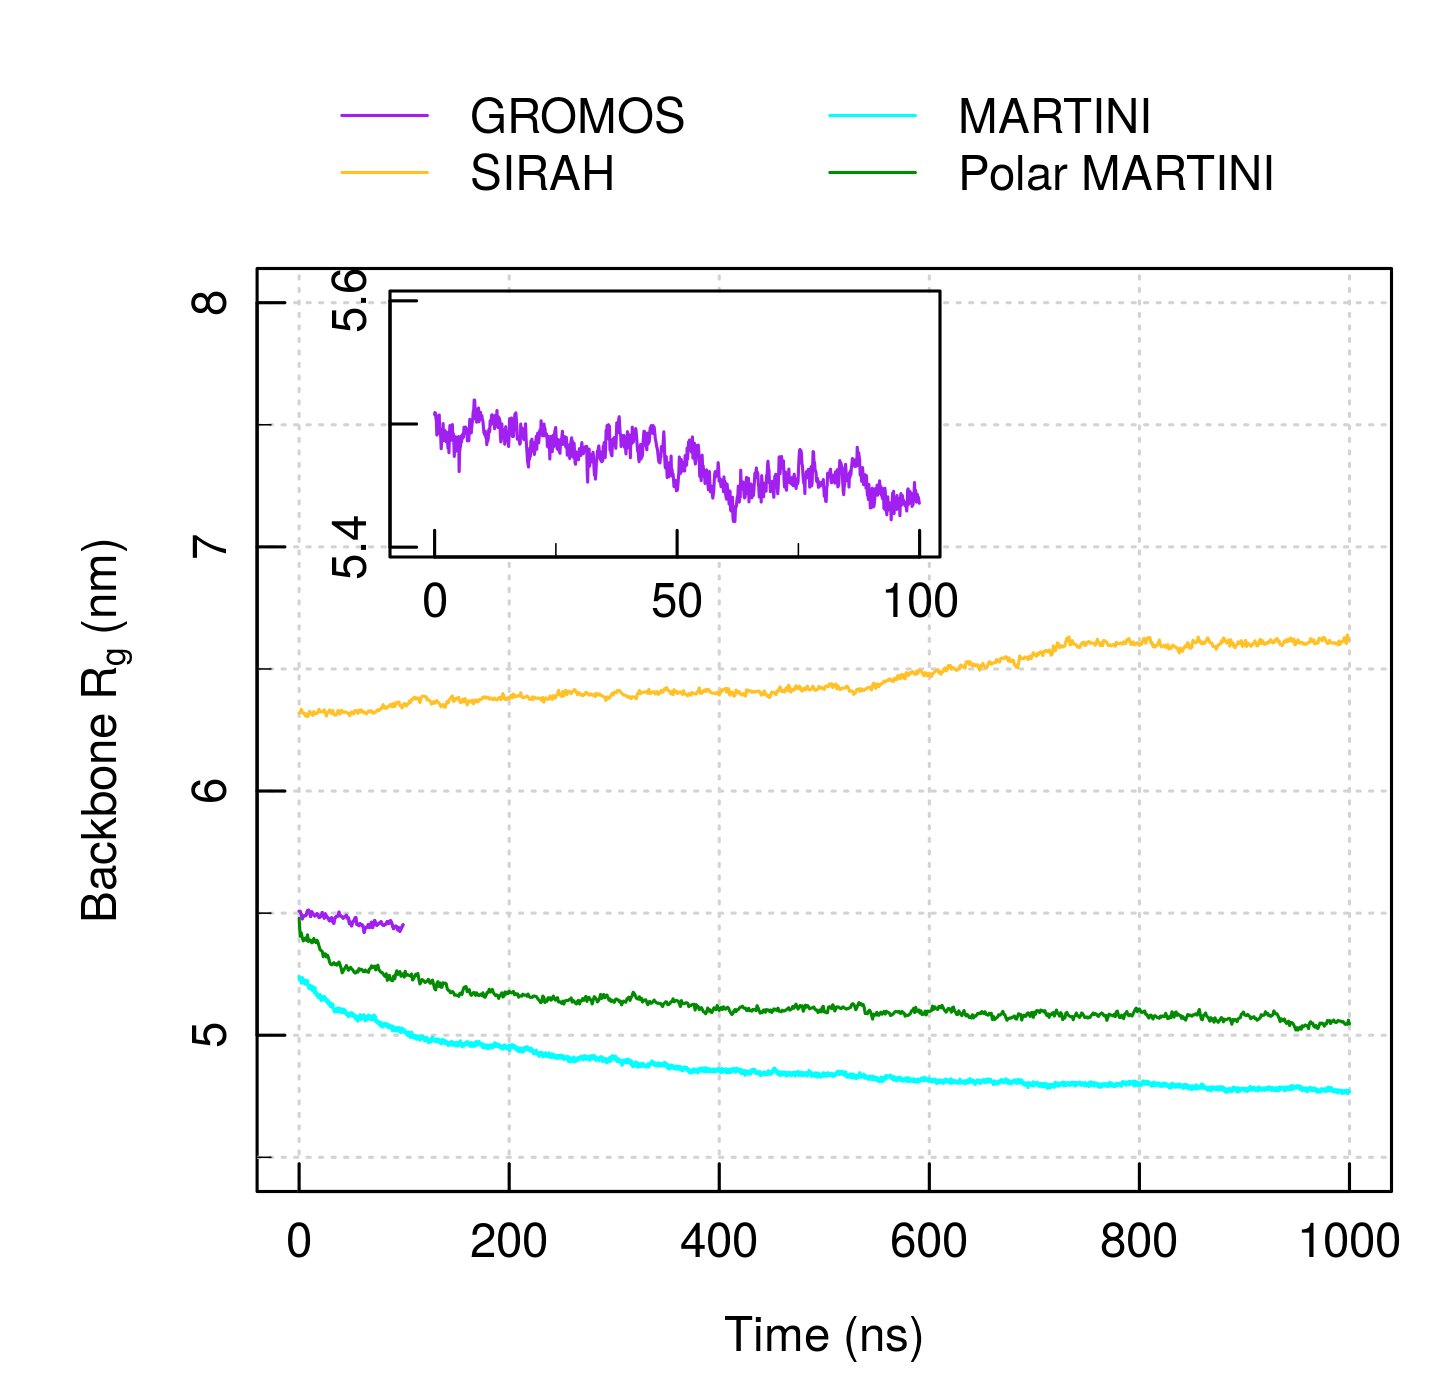
\includegraphics[width=0.48\linewidth]{3results_capsule/pics/Rg_all.png} \label{fig:Rg}} 
\subbottom[]{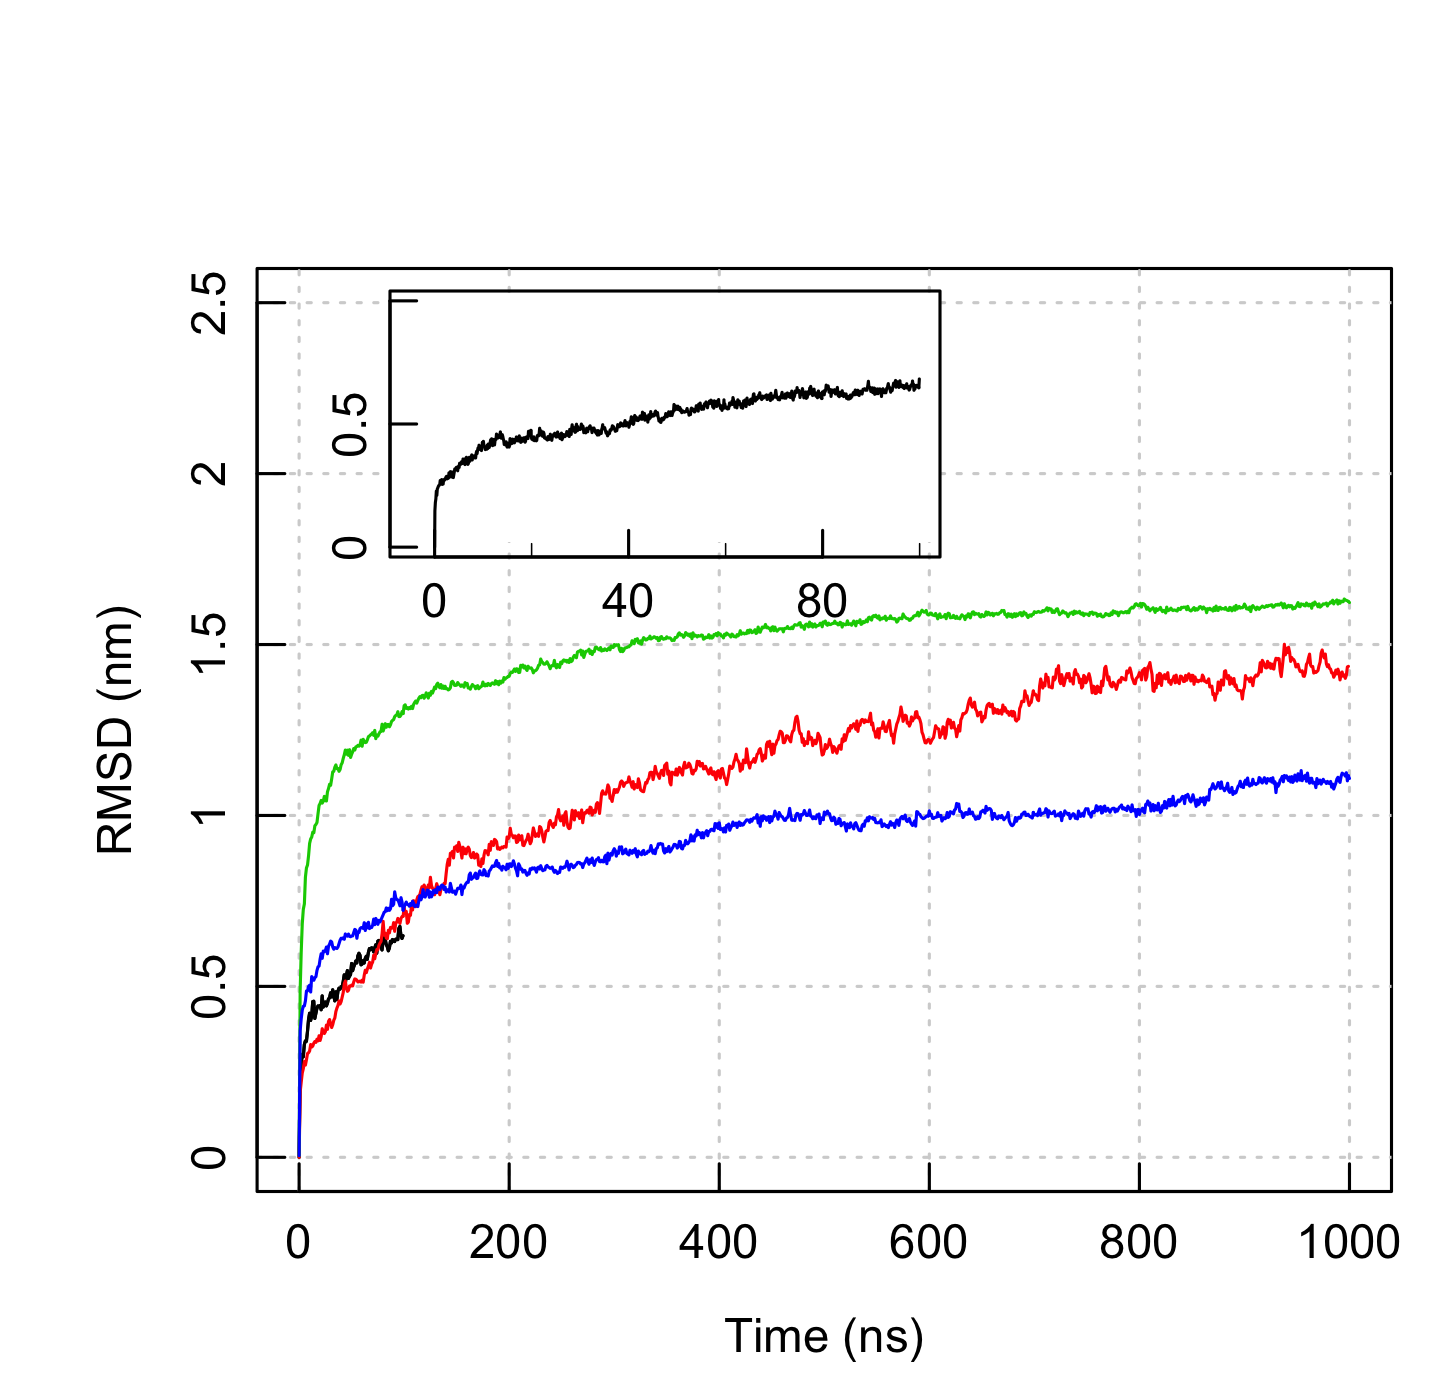
\includegraphics[width=0.48\linewidth]{3results_capsule/pics/RMSD_all.png} \label{fig:RMSD}} \\
\subbottom[]{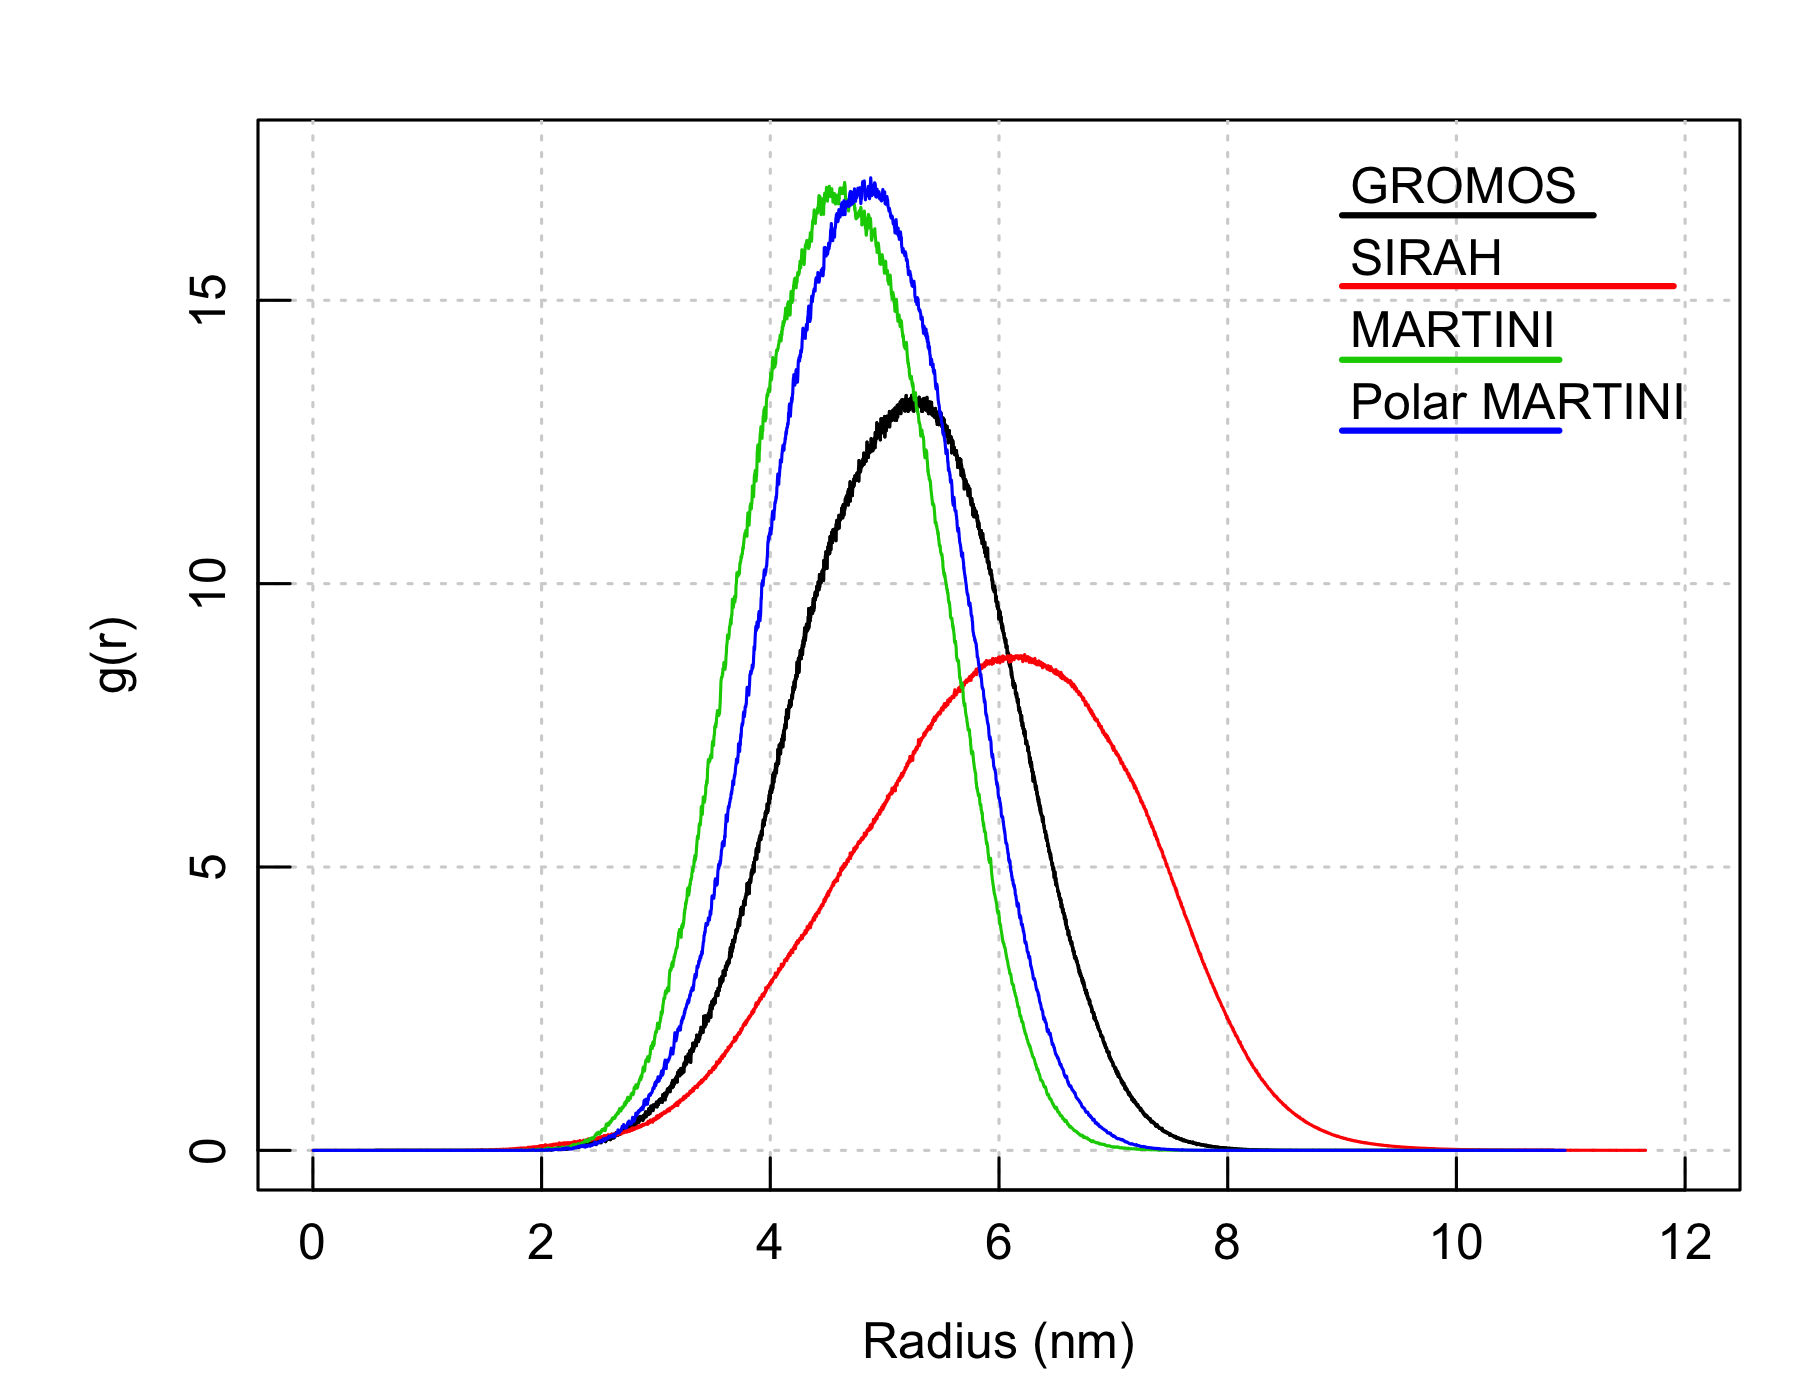
\includegraphics[width=0.48\linewidth]{3results_capsule/pics/RDF_all.png} \label{fig:RDF}}
\caption[Structural measures on buckyball in solution]{(a) R$_g$ and (b) RMSD computed on the Protein backbone. Results are displayed for simulations performed in GROMOS (100 ns), SIRAH, MARTINI and MARTINI with polar water (all 1 $\mu$s). Inset: zoom on the GROMOS values. (c) RDF of Protein masses around their center of mass, displayed for the same simulation set up as in (a,b). For each label of the legend, the bar has length of the respective FWHM of the Gaussian function fitting the data (thickness estimate). All results are showed for Replica 1 of each simulation set-up.}
\label{fig:struct_UA_SIhere}
\end{figure}
%
\paragraph{Global capsule structure} Atomistic simulations of the buckyball in solution show a consistently equilibrated structure across the three replicas run (Figure \ref{fig:BTI_snap} and SI movie 1).
%
This is proven by both the stable value of the protein R$_g$ and the almost plateauing backbone RMSD (Figure \ref{fig:Rg} and \subcaptionref{fig:RMSD}). It is interesting to notice that previous simulations performed with a shorter equilibration, without the phase of employing flat bottom restraints, lead to the immediate disruption of several connections in the buckyball network, resulting in larger R$_g$. This suggests that the structural pairing present in the buckyball can form only when the chains are in close contact. This is compatible with the long time of assembly observed experimentally (up to 7-10 hours): the closer the chains need to be to trigger the assembly, the rarer this event is statistically happening. Also, this implicitly proves that the self-assembly simulations starting from disordered states will not lead easily to such ordered configurations.

The RDF of the protein masses around the buckyball centre shows no masses nearby the origin (Figure \ref{fig:RDF}) and this means that the buckyball remains hollow (given the way RDF is computed and normalised, a uniformly full object would display a flat distribution).
%
A fit of the RDF to a Gaussian curve returns a mean value of 5.1 nm and a FWHM of 2.2 nm, which gives an estimate of the bilayer thickness.
%
A similar computation is repeated for the inner and outer layer separately, providing 1.1 nm of distance between the means of the two distributions. This interlayer distance is compatible with the one between the backbones of stacking $\beta$-sheet in structures like densely packed amyloids (1.0 nm \citep{Sunde1997}).

\begin{figure}[t]
\centering
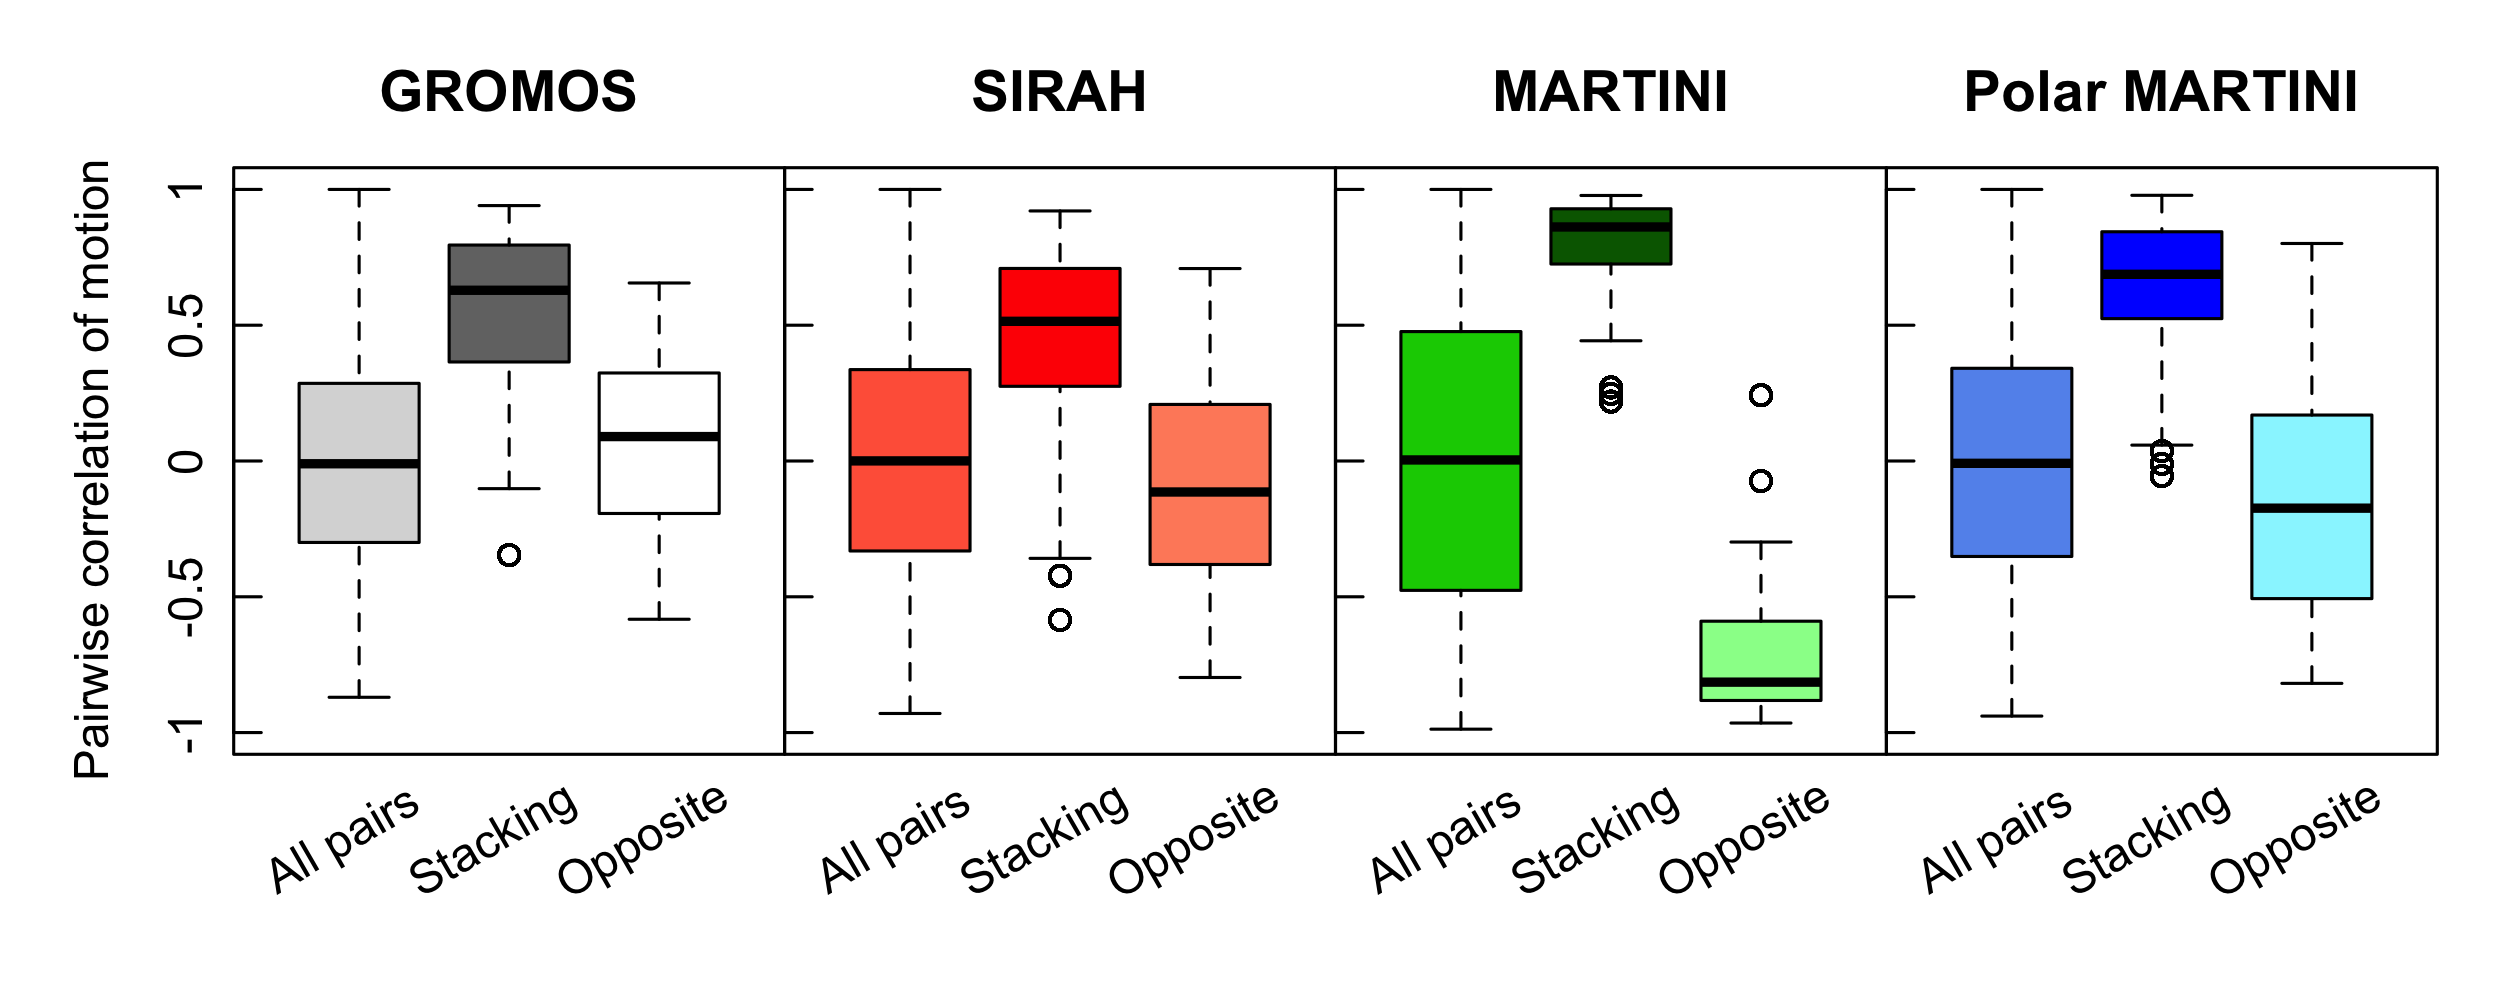
\includegraphics[width=0.95\linewidth]{3results_capsule/pics/RKGBcorr_boxplot_all.png} 
\caption[Correlation of motion between molecules of the buckyball]{Distribution of the correlation of motion between different molecules in the buckyball simulations. Black band: median of the distribution; box: first and third quartiles; whiskers: maximum and minimum, outliers excluded (hollow dots). Results are shown for Replica 1 of each simulation set-up.}
\label{fig:BTI_corr}
\end{figure}
%
This thickness value hints at the fact that the two layers are closely packed. This is confirmed by the analysis of the pairwise correlations of motion:
%
molecules at the same polar coordinates (i.e.\ stacking radially one on the other) have a positive correlation and so move coherently, while the ones at opposite poles, as well as the ensemble of all possible pairs, do not show particular correlation (Figure \ref{fig:BTI_corr}). 

\paragraph{Contacts between arms} The measure of how many arms in the buckyball network remain paired for more than 90\% of the simulation time is shown in Figure \ref{fig:BTI_beta}. An average of 160 pairings is observed between arms belonging to the same layer (summing over inner and outer), and around 20 only for inter-layer ones.
%
This first value correspond to slightly less than 3 pairing per molecule, which would be the value in a perfectly icosahedral structure. This 10\% reduction of the arms shows that the structure is not rigid, and some pairings are lost, but nevertheless it maintains the majority of its network of interaction in place.
%
On the contrary, few inter layer contacts are observed within 1.2 nm distance cut off: the arms belonging to two different layers are separated by the space spanned by their side chains, and this keeps the average positions of their backbones at a distance greater than the cut off chosen.
%
\begin{figure}[t!]
\centering
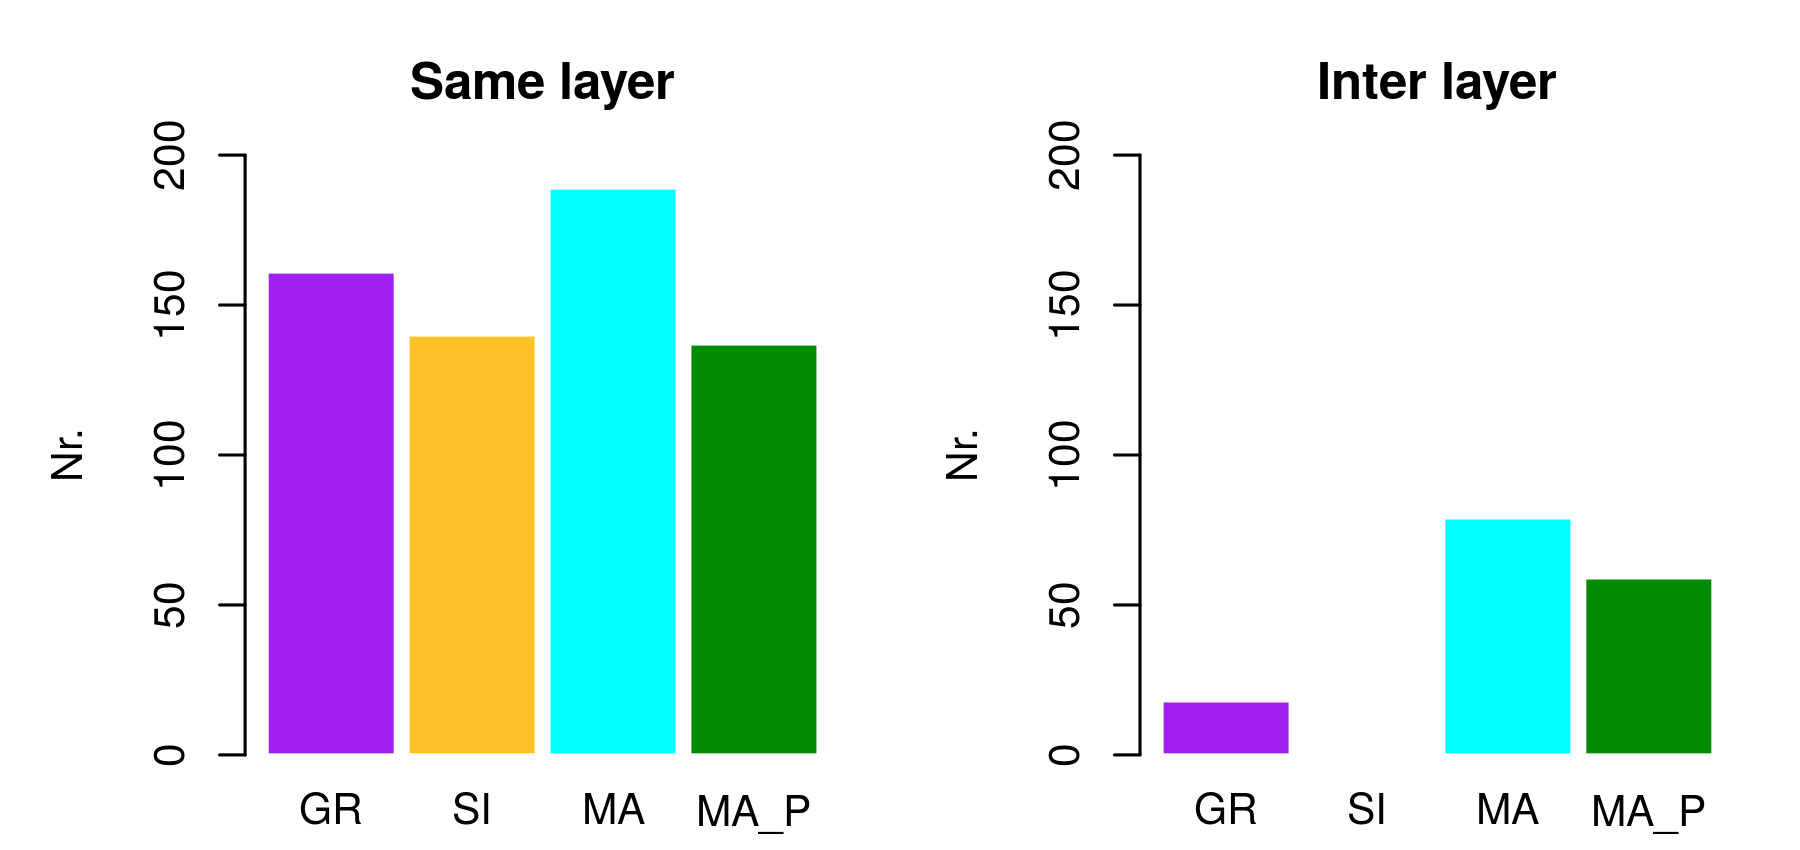
\includegraphics[width=0.85\linewidth]{3results_capsule/pics/stAll_beta_90_R1.png}
\caption[Arm pairing during simulations of the buckyball]{Number of paired arms within the same layer and between layers. Cut off distance between arms center of mass equal to 1.2 nm. Only contacts existing more than 90\% of the simulation time are counted. Results are shown for Replica 1 of each simulation set-up.}
\label{fig:BTI_beta}
\end{figure}

\begin{figure}[p!]
\centering
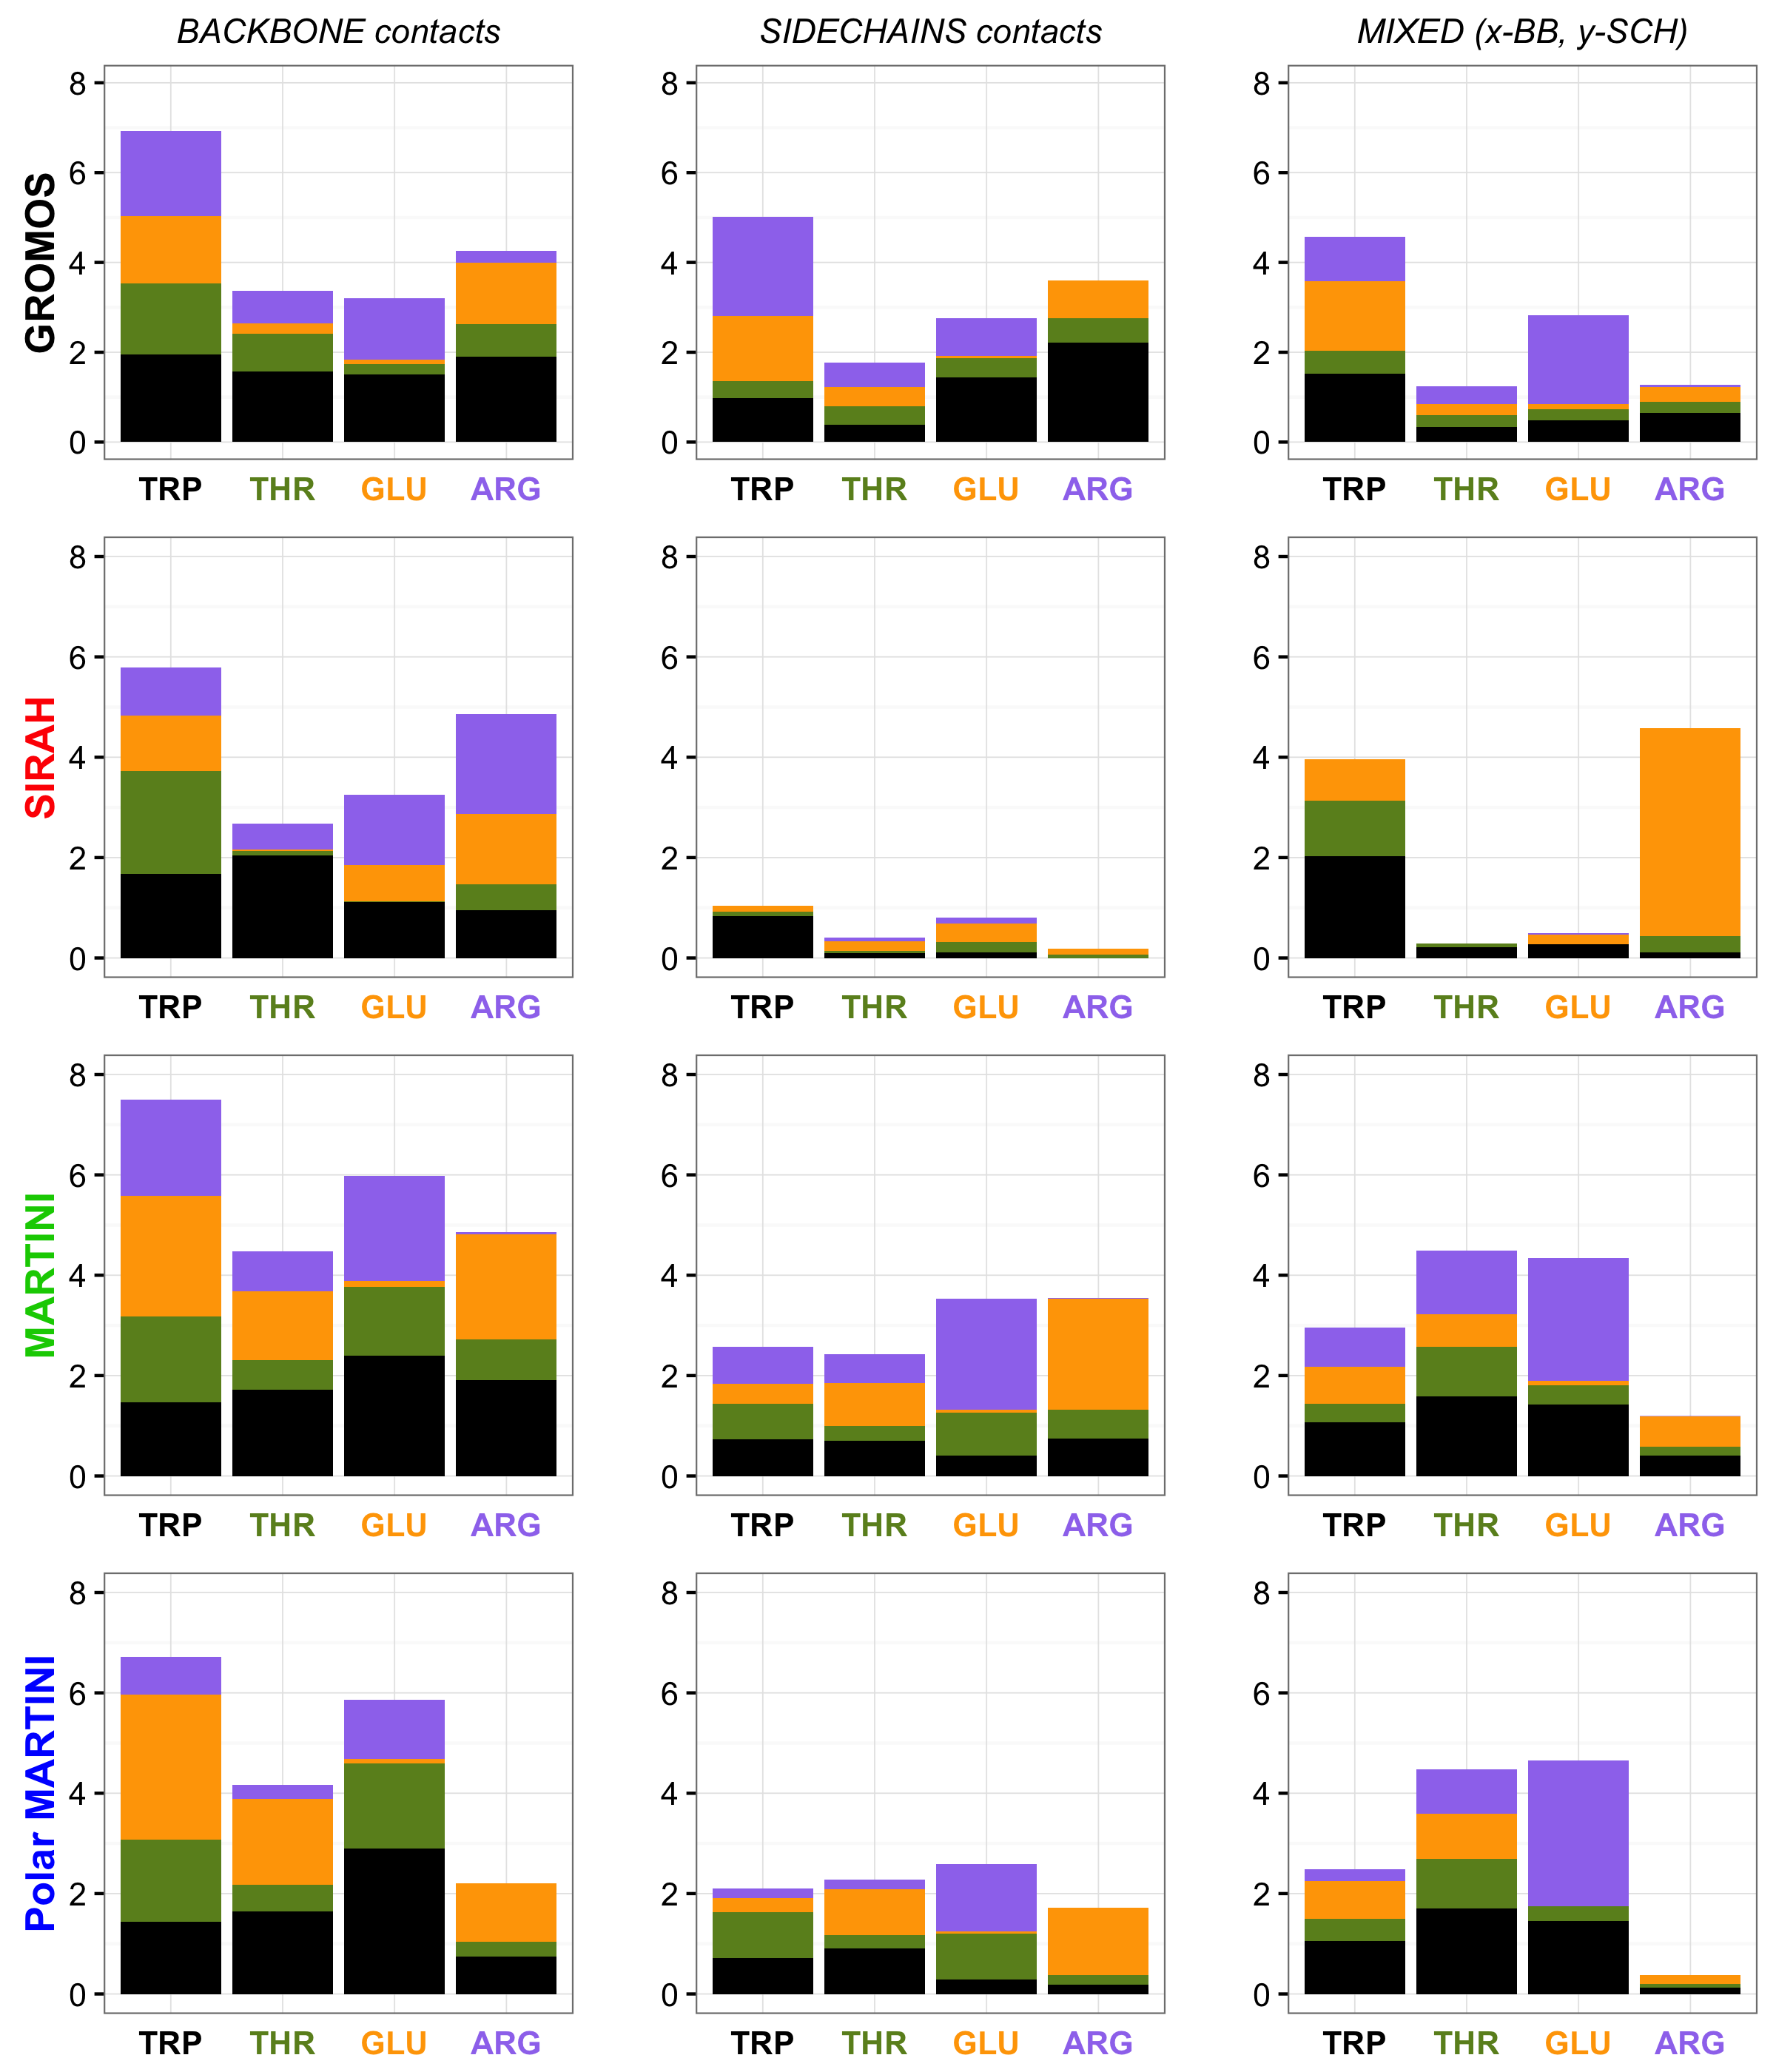
\includegraphics[width=0.95\linewidth]{3results_capsule/pics/new_rep1_allFF.png}
\caption[Contacts between buckyball molecules]{Number of contacts per residue type in each arm of capzip: each bar shows the average number for the residue on the $x$-axis; its color is split by the identity of the partner residue (color coded as in the $x$-axis legend). For mixed contacts the residue on the $x$-axis contributes with its backbone. The parametrisation is reported along the $y$-axis. Results are shown for Replica 1 of each simulation set-up. Only contacts existing more than 50\% of the simulation time are considered.}
\label{fig:BTI_cont}
\end{figure}

\paragraph{Contacts between residues} Figure \ref{fig:BTI_cont} shows the number of contacts between backbones and/or side chains of amino acids which survive more that 50\% of the simulation time. They are classified by amino acid type and normalised over the number of residues present for each type (so this takes already into account the fact that there are two Arg and Trp per arm of capzip, but one Thr and Glu only).

The number of backbone contacts per residue is around 1 for Threonine (Thr) and Glutamic acid (Glu), 0.7 for Arginine (Arg), and 1.2 for Tryptophan (Trp) residues (Figure \ref{fig:BTI_vmd}, B).
%
Thus, on average each residue is paired with another one, except for Arginines: only two thirds of them are engaged, likely because some Arg residues are at a terminal positions, and as such they tend to extend in solution, unpaired. On the contrary, Tryptophan is more prone to form contacts, because of its hydrophobic character and central position in the sequence.

The bar plot shows also that there is no strictly fixed arrangement between arms: for example, Tryptophan residues are not paired mainly to Tryptophan ones, as the optimal arrangement would dictate, suggesting flexibility in the structure.
%
Nevertheless, this specific residue has clearly a prominent role in forming contacts with the neighbours both at the backbone level and at the side chains one through cation-$\pi$ interaction with Arginine (central column of Figure \ref{fig:BTI_cont}).

\paragraph{Hydrogen bonds interaction} Some of the contacts mentioned above are mediated by hydrogen bond interactions, so the average number of inter molecular hydrogen bonds occurring during the simulations is computed, divided by the number of molecules and classified by residue type.
% SAY THAT THEY ARE THE ONE OCCURRING AT ANY MOMENT, AND NOT THE ONES SURVIVING MORE THAN 50%?
We further separate the hydrogen bonds occurring between backbones and/or side chains. Tryptophan contributes to a large number of backbone hydrogen bonds (Figure \ref{fig:BTI_hbonds}, A), especially with other Tryoptophan residues, consistently with what found in the analysis of contacts carried on previously. Arginine side chains are the most prone to establish H-bonds as a donor with many different amino acid side chains (Figure \ref{fig:BTI_hbonds}, B), but especially with Glutamic acid as expected from the facing positions they occupy in the network arrangement and their opposite charges which attract them closer.
%
Similarly, a common interactions is between Arg side chain (donor) and Glu backbone (Figure \ref{fig:BTI_hbonds}, C), and between Arg backbone (donor) and most of the other side chains (Figure \ref{fig:BTI_hbonds}, D).
\begin{figure}[t]
\centering
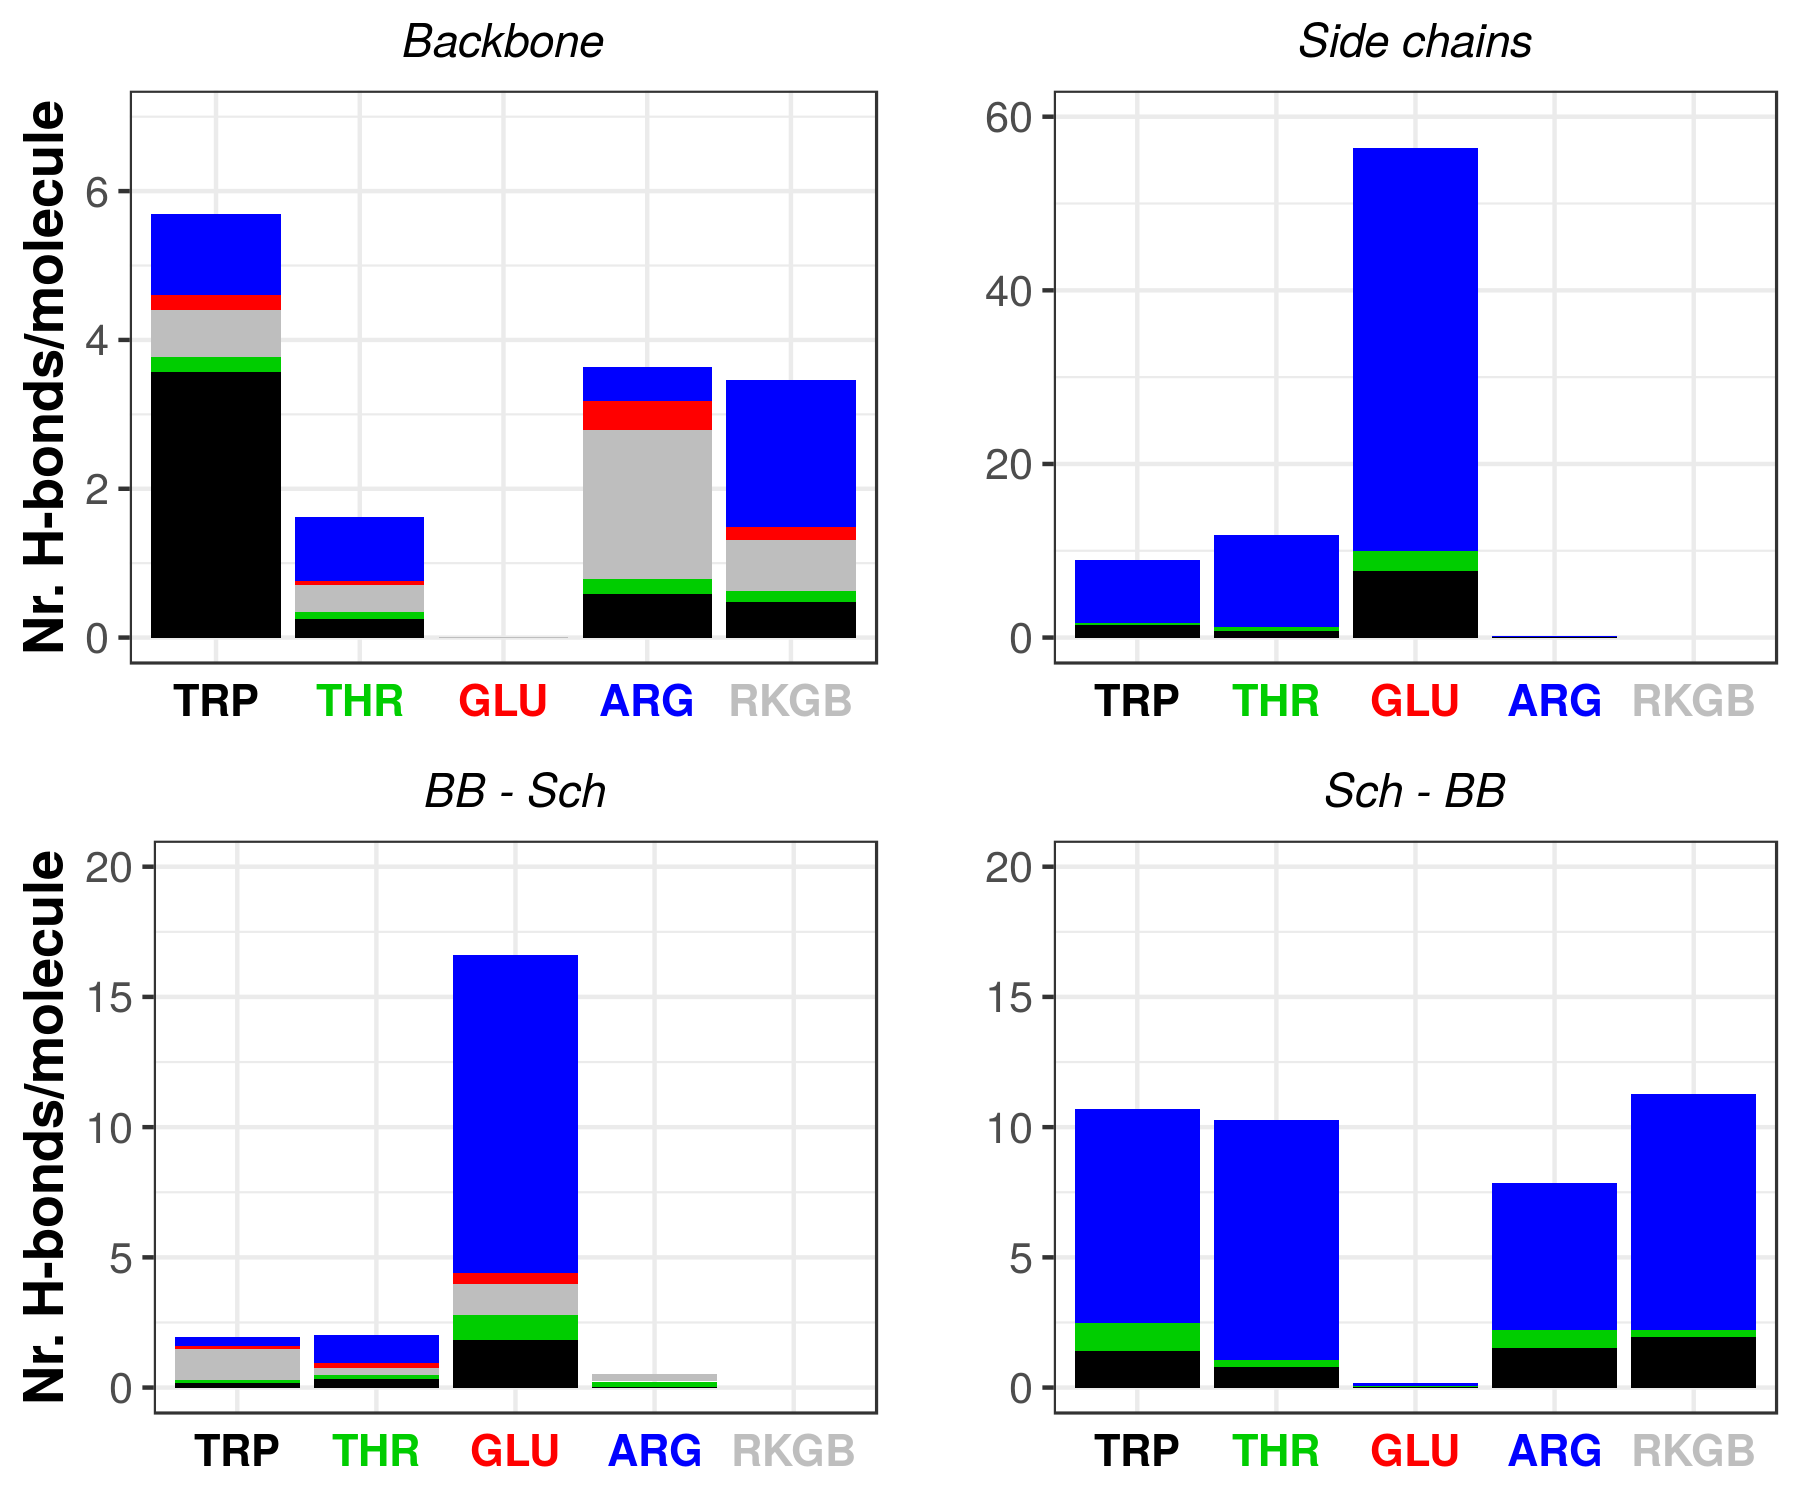
\includegraphics[width=0.85\linewidth]{3results_capsule/pics/Hb_all.png} 
\caption[Hydrogen bonds between molecules in the buckyball]{Average number of hydrogen bonds per residue occurring between amino acids, including the central scaffold RKGB, for a 100 ns atomistic simulation of the buckyball in solution. Result are shown for Replica 1. For each bar, the residue on the $x$-axis is the acceptor, and the bar is split by the identity of the donors. In the case of Backbone - Side chain and Side chain - backbone, the first mentioned correspond to the acceptor (and thus the residue on the $x$-axis).}
\label{fig:BTI_hbonds}
\end{figure}

\paragraph{Chemical characteristics of the surface: SASA} Finally, it is important to understand what residues are exposed at the surface of the structure, especially in view of future applications: in order to make the peptide co-assemble with other products, the two must have a compatible chemical character. The average Solvent Accessible Surface Area (SASA) for every amino acid along capzip arm (Figure \ref{fig:BTI_sasa_exposed}) shows that half of the accessible surface is represented by the charged residues Arginine, while Tryptophan contribute to it for less than one quarter, despite having bulky side chains.
%
For atomistic simulations, we can compare the SASA of each residue of type X with the reference SASA computed by theoretical modelling of a Gly-X-Gly tripeptide \citep{Tien2013}. The resulting ratio $Q_{SASA}$ is greater than one for both the Arginines: while for the terminal one (ARG1) it is consistent with the absence of a residue on one of the sides, the fact that also the second has $Q_{SASA}>1$ proves that these residues are highly exposed in solution. On the contrary, Tryptophan has values around $0.5$, due to its propensity to be buried inside the structure, while Glutamic acid and especially Threonine have value closer to one, showing no particular burying.
\begin{figure}[t]
\centering
\subbottom[]{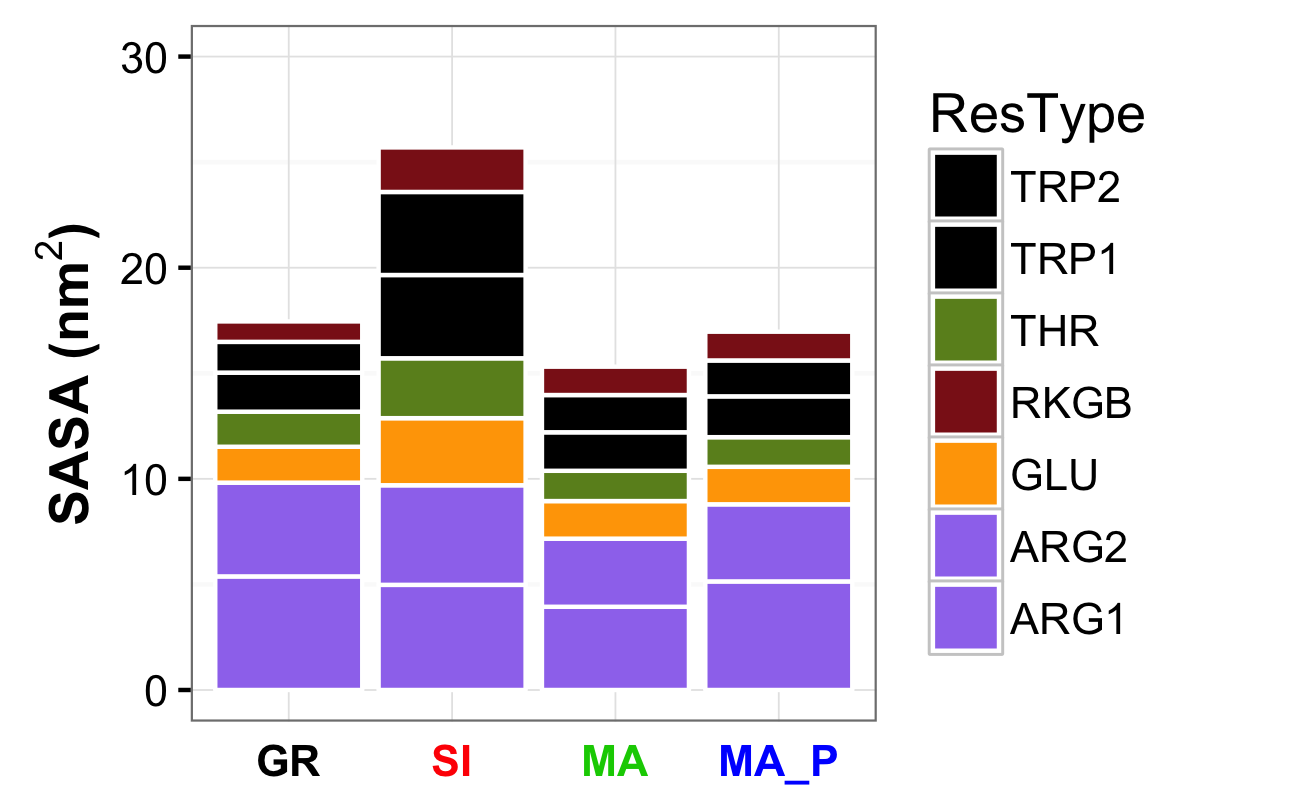
\includegraphics[height=0.3\linewidth]{3results_capsule/pics/st_All_sasa_fractions.png} \label{fig:all_sasa}} 
\subbottom[]{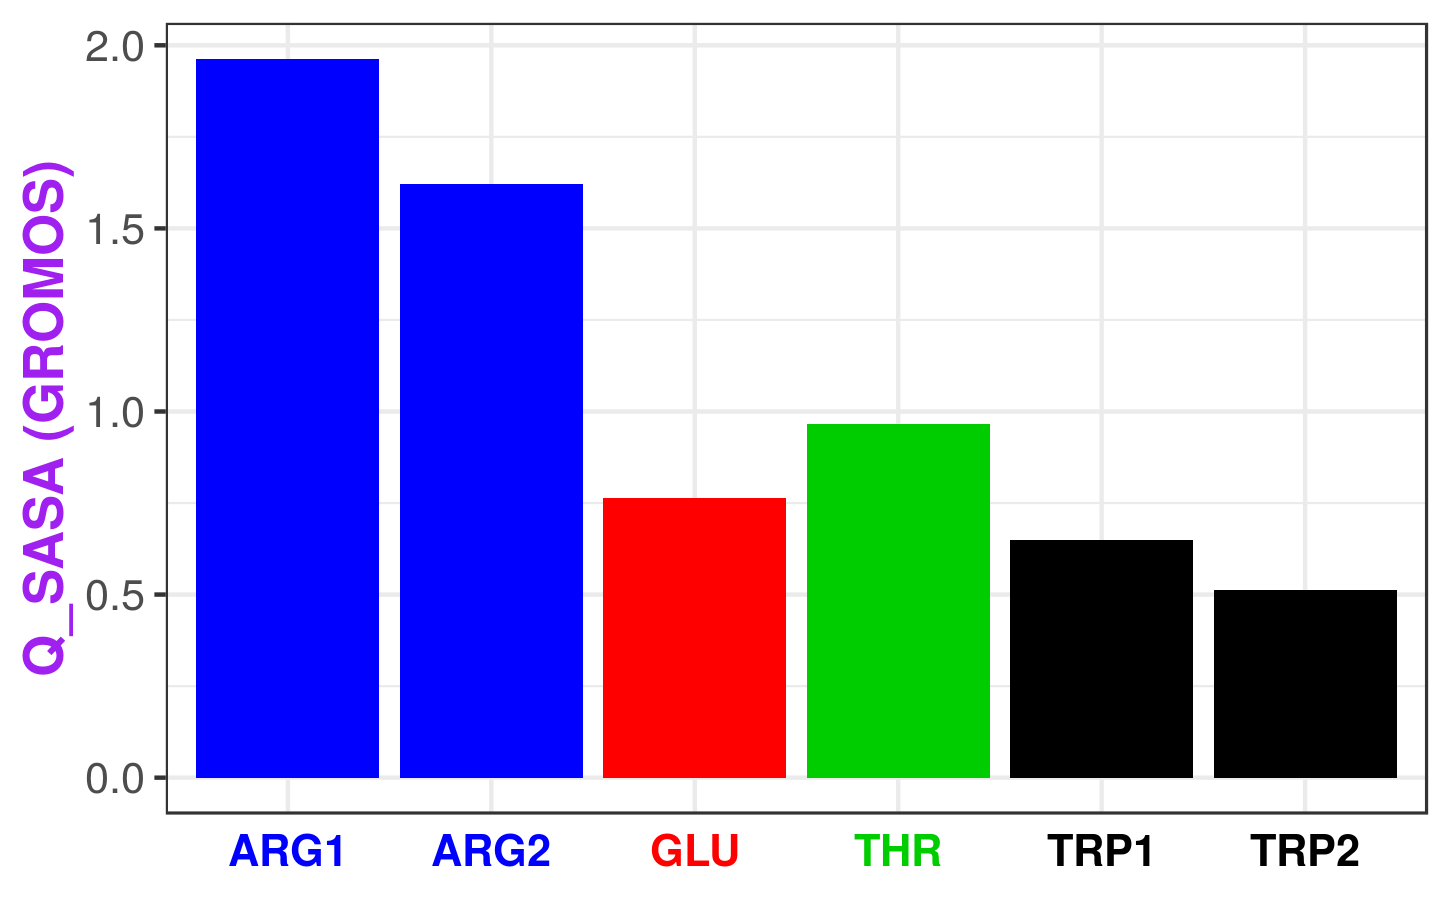
\includegraphics[height=0.3\linewidth]{3results_capsule/pics/st_Qsasa.png} \label{fig:Q_sasa}} 
\caption[SASA per residue of a buckyball in solution]{(a) Solvent Accessible Surface Area (SASA) per molecule, divided by residue types. Results are shown for Replica 1 of each simulation set-up. (b) Normalised SASA over the reference SASA computed for each amino acid type X as the value in a Gly-X-Gly tripeptide.}
\label{fig:BTI_sasa_exposed}
\end{figure}

\paragraph{D-amino acids} The results presented above are derived from simulations of the capsule composed by standard amino acid (L-form). As explained in Chapter \ref{chapter:intro}, some experiments focussed on the opposite chiral form (D-version) for stability and immunogenicity reasons. Experimental work shows similar behaviour for the two enantioners in solution, because they are mirror images of each other.

Accordingly, simulations of D-amino acids should not give any discrepancy with what found before. As a control, we performed one run with such mirror system - and suitable amino acids parameters to keep the D-chirality - finding a similar behaviour of the capsule (i.e.\ differing from the L- simulations as much as the L- replicas differ among them - Figure \ref{fig:D_aa}).

\begin{figure}[t]
\centering
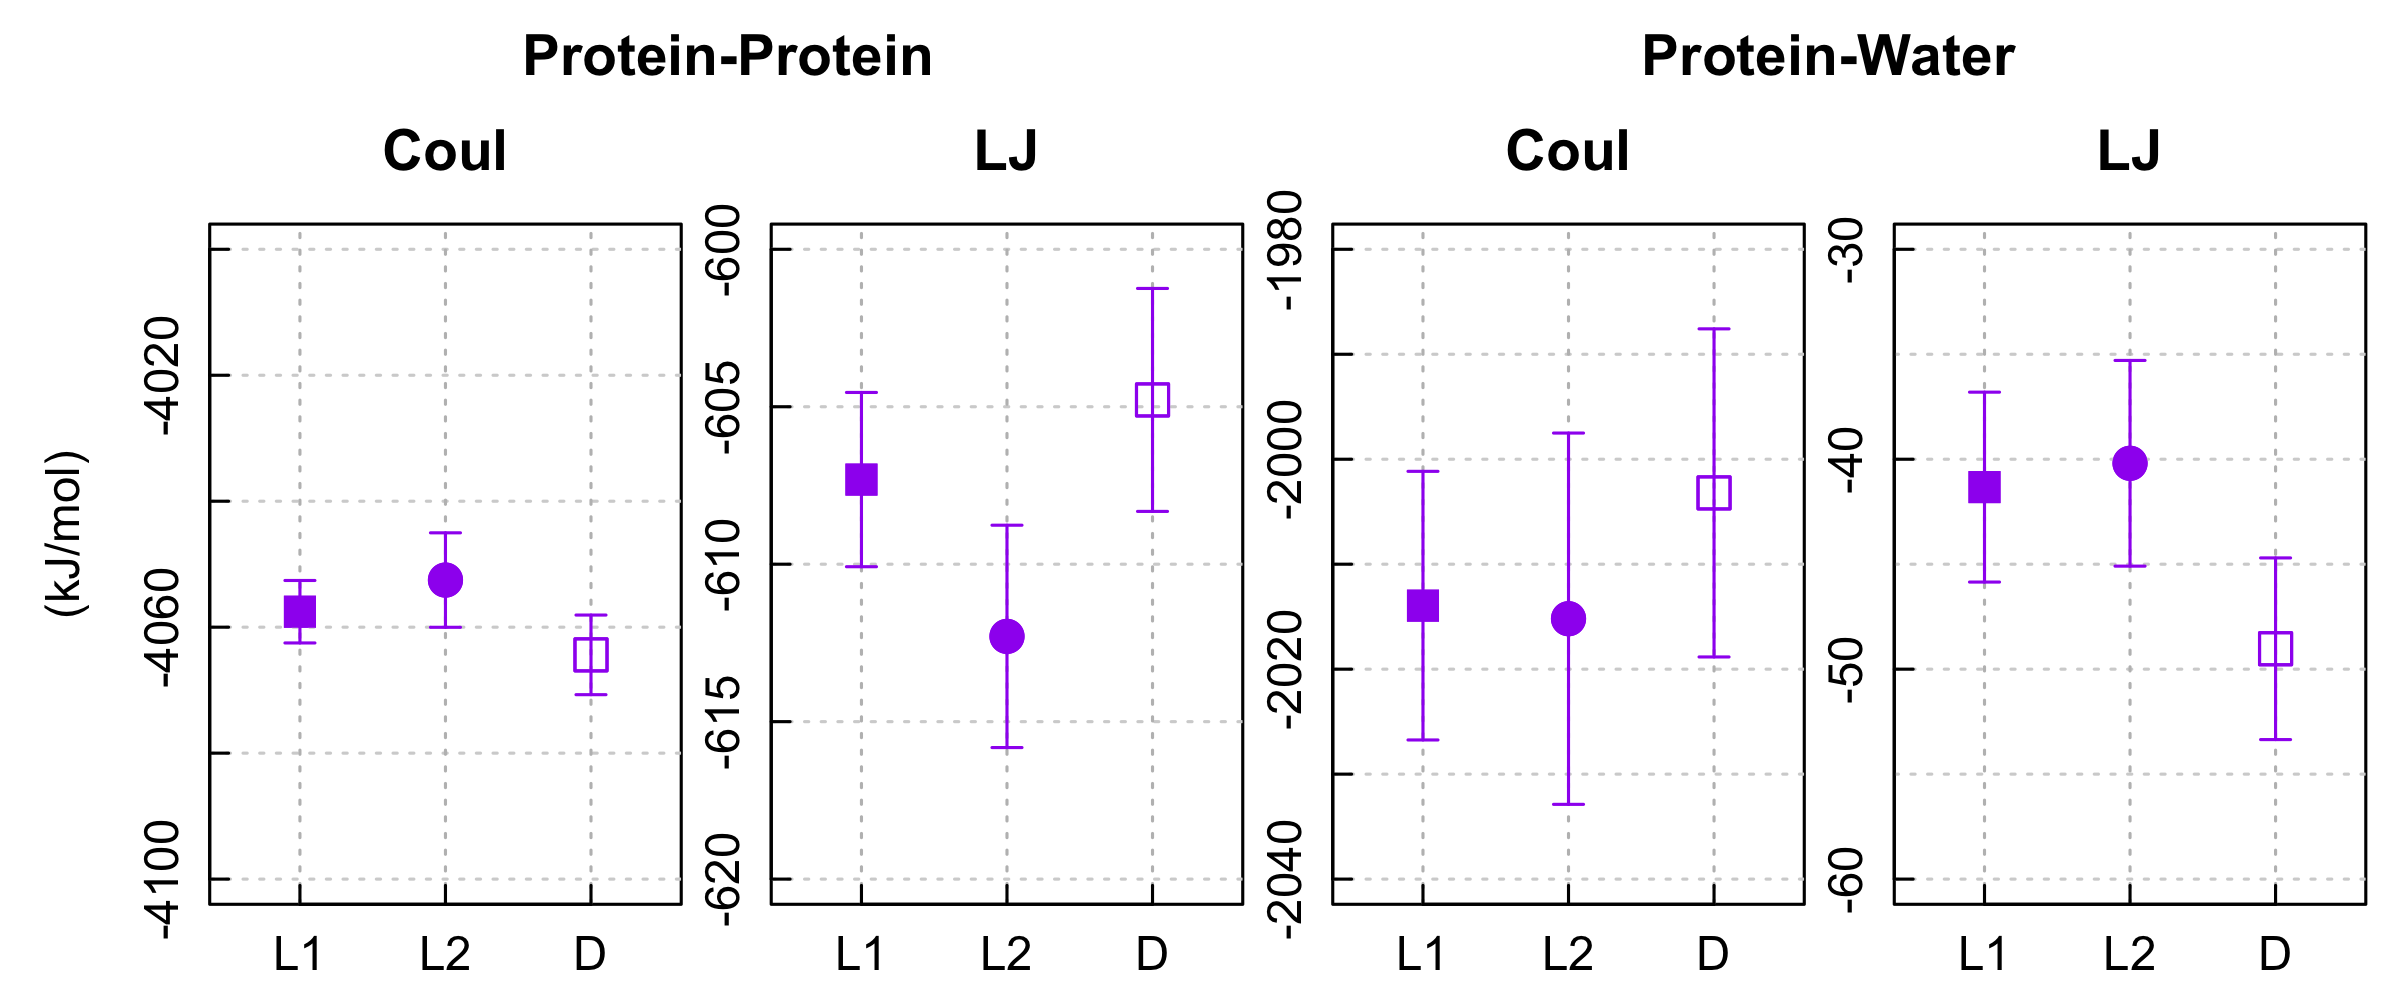
\includegraphics[width=0.95\linewidth]{3results_capsule/pics/compare_D_L.png}
\caption[Energies of L- and D-amino acids buckyball bilayer (atomistic)]{Energies of L- and D-amino acids buckyball bilayer. Average values for the second half of the simulation. Two replicas are shown for L-amino acids (L1 and L2), one only was run for D-amino acid (D).}
\label{fig:D_aa}
\end{figure}

This investigation can be performed only at the atomistic level as the coarse-grained models employed represent the C$^\alpha$ and the hydrogen attached to it as a unique bead, loosing then the chirality of this centre.


\subsection{Multiscale comparison of model capsule} \label{sec:res_multiscale}

We performed a multiscale analysis simulating the capsule structure with different coarse-grained force fields, with a twofold aim: first we wanted to simulate the assembly for a longer time, to observe how its structural properties are maintained on the medium time scale (of the order of the microsecond). Second, we believe that proving the stability of the capsule with different descriptions strengthens the evidence that the assembly proposed is indeed a favourable arrangement of the molecules in solution.

As mentioned before, to this aim we compared simulations run with the SIRAH, MARTINI force fields and MARTINI used in conjunction with polar water (Polar MARTINI). The investigation is also useful to elucidate where the descriptions differ and to infer the advantages of each model.
%
We first comment on the quantities already analysed at the atomistic level (if applicable), and then we extend the analysis to simulations of a monolayer capsule, which has been modelled to verify whether the hypothesis that a bilayer structure is necessary to grant stability was true.

\paragraph{Coarse-grained global structures}
As foreseeable, the structures obtained with coarse-grained force fields are slightly different among each other and with respect to the atomistic one.
%
The SIRAH bilayer capsule has a structure more expanded with respect to the atomistic one, with a skewed and broader RDF profile, while MARTINI provides a more compact configuration, and finally Polar MARTINI a slightly more expanded structure than standard MARTINI, with a comparable thickness. Respectively, for SIRAH, MARTINI and Polar MARTINI the average radius is 6.0 nm, 4.6 nm and 4.8 nm, with 2.9 nm, 1.9 nm and 1.9 nm average thickness - see Figure \ref{fig:Rg} and \subcaptionref{fig:RDF}.
%
The difference between the two MARTINI models is likely due to the better properties of solvation of charged groups in the Polar MARTINI description \citep{Yesylevskyy2010}, united with the fact that the buckyball contains a high number of them.

The correlation of motion between molecules for all the coarse-grained force fields is similar to the atomistic one, with a slight anticorrelation between molecules at the opposite poles for MARTINI and Polar MARTINI (Figure \ref{fig:BTI_corr}). This is due to the contraction happening at the beginning of the simulation, when the capsule adjusts to the equilibrium size, which depends to some extent on the force field.
%
These effects are more pronounced for the MARTINI force fields, probably due to the greater cohesion between the beads which makes them moving coherently.

% CONTACTS:
%			GR		SI		MA		MAP
% SAME 		161,		140, 	189, 	137
% INTER 		18, 		1, 		79, 		59
\paragraph{Coarse-grained contacts analysis}
The number of chains paired in the SIRAH simulations is fewer than in the atomistic ones (Figure \ref{fig:BTI_beta}), in line with a more expanded structure, while MARTINI simulations propose a higher number, consistently with the reduced size of the capsule. In particular, the contacts between the two layers are significantly higher in MARTINI. This is expected when the two layers are closer, as suggested by the values of the stacking molecules correlation. Finally, Polar MARTINI agrees with the high number of inter layer contacts of MARTINI, but suggests a partial loss of contacts within the same layer. However, as the structure is compact, the overall shape is still maintained, even without such precise pairing of the arms.

Breaking down the contact analysis by residue type (Figure \ref{fig:BTI_cont}), each coarse-grained force field shows a different organisation due to the models of the side chains volumes, which thus occupy a different fraction of the space available.
%
Nevertheless, in all the representations, Tryoptophan has a prominent role in establishing contacts with its neighbours at the backbone level, while different force field disagree on the role of the side chains. Quite surprisingly, the SIRAH force field does not promote interactions between side chains a part from the Tryptophan ones with themselves. This seems due to the more expanded structure of the capsule and consistent with the larger solvation of the amino acids, which are more exposed in solution (see next paragraph discussing SASA values).
%
Finally, none of the coarse-grained force fields seem to capture the preferential cation-$\pi$ interaction between Arginine and Tryptophan, as can be expected from a less detailed description.

\paragraph{Coarse-grained SASA} The values of SASA cannot be compared between force fields, because of the different dimensions of the beads and the number of them employed to describe the residues. However, it is interesting to notice that consistently across force fields, Arginine constitutes around half of the exposed surface, with the exception of SIRAH, where the more expanded structure results in all the residues to be quite exposed (Figure \ref{fig:all_sasa}). This confirms that these charged residues are more exposed in solution, while Tryptophan ones are buried.

\paragraph{Energetic profile} The above results point out that every coarse-grained force field has a particular propensity for an equilibrium distance between peptidic components. This is due to the different solvation property of the water model chosen, and to the balance between the different components of the energy. To better understand this, we computed the Coulomb and Lennard-Jones contribution to the energy due to Protein-Protein interactions or Protein-Water ones.
%
Figure \ref{fig:value_eng_cg} plots these values averaged over the second half of the simulated time for the atomistic and each coarse-grained force field (for atomistic and SIRAH description the Protein-Protein terms include both the short range interactions and the 1-4 interactions, i.e.\ the ones computed between atoms separated by three bonds, as they are computed separately during the simulations. For MARTINI models instead they are grouped together in the short range term).

\begin{figure}[h!]
\centering
\vspace{3cm}
\subbottom[]{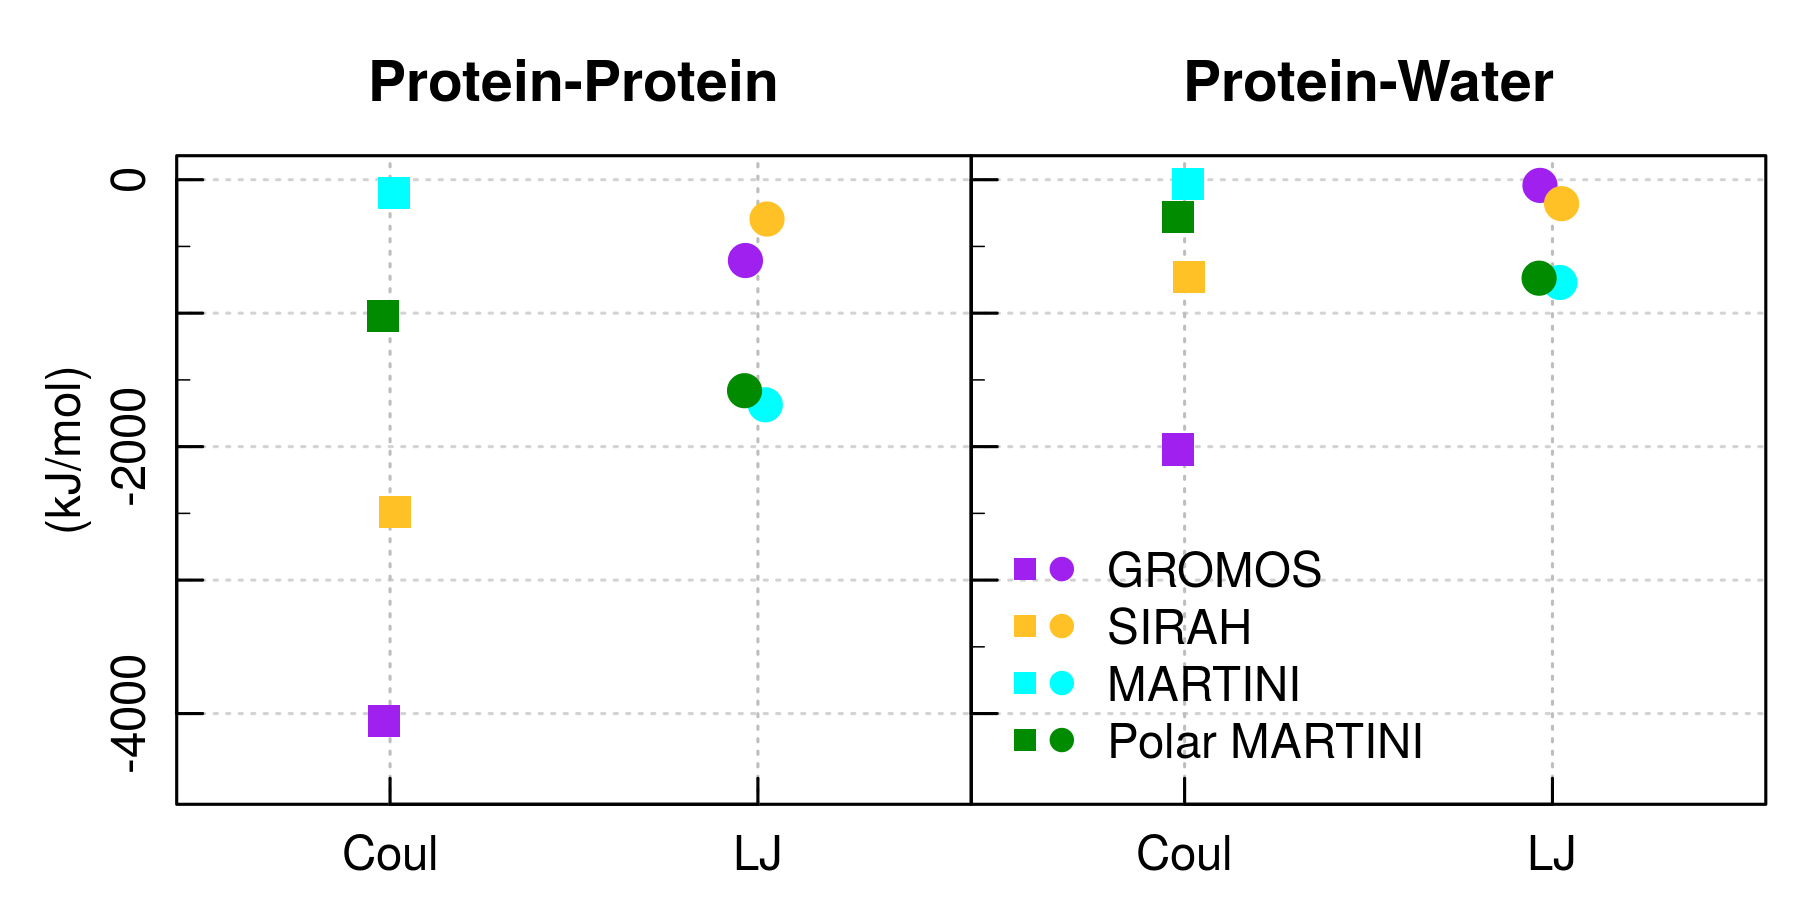
\includegraphics[width=0.8\linewidth]{3results_capsule/pics/many_energies_brief.png} \label{fig:value_eng_cg}} 
\subbottom[]{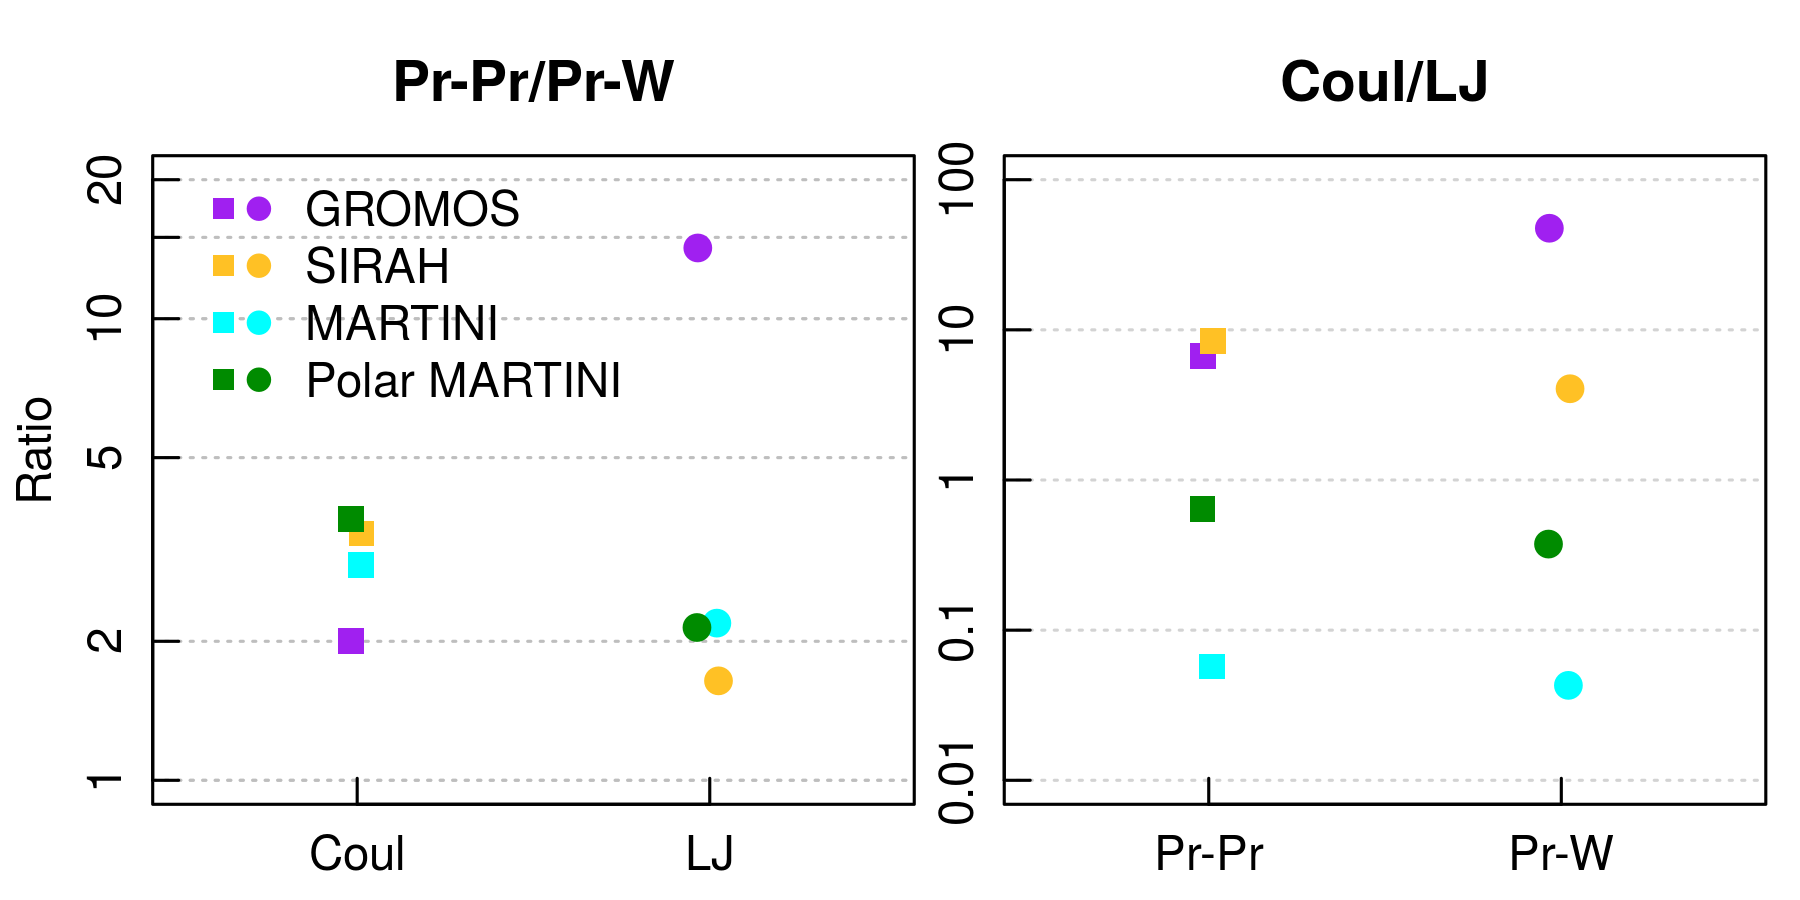
\includegraphics[width=0.8\linewidth]{3results_capsule/pics/ratio_energies_brief.png} \label{fig:ratio_eng_cg}} 
\caption[Non-bonded protein energy contribution to buckyball bilayer structures]{(a) Protein-Protein and Protein-Water non-bonded interactions, normalised per molecule. Values obtained as average on the second half of the trajectory of Replica 1 for each simulations set-up. (b) Ratio between the Protein-Protein and Protein-Water interactions for each force field, for Coulomb and Lennard-Jones respectively; or between Coulomb and Lennard/Jones, for Protein-Protein an Protein-Water interactions separately (note the log scale on $y$). Values computed as for plot (a). Points are misaligned along $x$ to facilitate the reading.}
\label{fig:eng_cg}
\vspace{3cm}
\end{figure}

Considering the Coulomb component, it is clear that the mean field approach of standard MARTINI, which consists in adopting a high relative dielectric constant ($\epsilon = 15$) to compensate the absence of water dipoles, decreases sensibly the contribution of the Protein-Protein electrostatics with respect to the two other models.
%
This approach reduces all the Coulomb interactions, while in reality the screening effect due to the water can be seen only, e.g., on distances larger than about 1 nm in a 0.1 M salt solution. This simplified approach instead screens also the contribution of two nearby atoms separated by a distance less than the size of a water molecule. Due to the $r^{-6}$ behaviour of the Coulomb interaction, these short scale contributions are clearly important for the total Coulomb energy.
%
The partial reversion to $\epsilon = 2.5$ performed by Polar MARTINI, together with the introduction of a water dipole, increases the amount of the Coulomb contribution by 10-fold (in absolute value).
%
Interestingly, this is higher than the ratio $\epsilon_{standard}/\epsilon_{Polar} \sim 6$, likely because the reduced short range screening also allows a stronger interactions between opposite charges, bringing them closer and thus contributing more (negatively) to the Coulomb energy.

SIRAH simulations instead are run at $\epsilon = 1$, and present a Coulomb component 2.5 times larger than the one of Polar MARTINI, suggesting that the two models give a similar energy contribution, which is then rescaled by their respective dielectric constant.
%
Finally, the atomistic model ($\epsilon = 1$) suggests even higher (in absolute value) Coulomb energy, roughly the double of SIRAH ones.

%Divided by correspondent atomistic value
%		SI			MA			MA_P
%C PP:	0.61443485 	0.02379733 	0.25118993 
%LJ PP:	0.4866778 	2.7857331 	2.6115072 
%C PW:	0.35982317 	0.01633541 	0.13665325
%LJ PW:	4.216698 	18.098146 	17.340699

These differences in Coulomb energies affects both the Protein-Protein and Protein-Water interactions consistently (Figure \ref{fig:ratio_eng_cg}, left), but they have consequences on the dynamics because they change the proportion of Coulomb energy with respect to the Lennard-Jones contribution (Figure \ref{fig:ratio_eng_cg}, right). These interactions are not changed between the two MARTINI models, making them predominant in standard MARTINI, where electrostatics are weak, while they are competing with the Coulomb contribution in Polar MARTINI.
%
On the contrary, SIRAH parametrisation opts for a smaller role of Lennard-Jones with respect to the Coulomb contribution, more consistently with the atomistic description, especially regarding the Protein-Protein interaction.
%
To recapitulate, protein electrostatics have an increasing contribution in MARTINI, Polar MARTINI, SIRAH and atomistic respectively, both in absolute terms and with respect to the Lennard-Jones contribution.

This might partially explain the differences in sizes observed across the models: for example the Protein-Protein Coulomb energy is more negative in SIRAH. However, with a smaller dielectric constant with respect to MARTINI, these contributions are less screened, thus the many positive amino acids composing the capsule (giving a positive net charge) can repel each other more effectively.

Comparing the two MARTINI models instead, Polar MARTINI has a greater Protein-Protein Coulomb component with respect to standard MARTINI (in absolute value, which means a more negative contribution). From this can be deduced that the slightly more expanded structure observed in Polar MARTINI is likely due to a different balance of electostatic versus Lennard-Jones, rather than to the more favourable solvation due to the polar water model.
%
Indeed, the balance between Protein-Protein and Protein-Water components (Figure \ref{fig:ratio_eng_cg}) is in the same range for all the three coarse-grained force fields, and it is slightly higher than the atomistic value for Coulomb, while for Lennard-Jones it is lower by about 15-fold.

An interesting follow up on this topic would be investigating whether a tuning of the dielectric constant used in the two MARTINI models can produce more consistent results between them. However, the choice of the constant was optimised to reproduce at best the properties of bulk water and solvation free energies of ions for both cases. This then raises the question whether the protein parametrisation performs equally good in conjunction with both model, or whether one reproduces better the atomistic Protein-Water interactions.


\subsection{Bilayer versus monolayer: coarse-grained simulations} \label{sec:mono}
To prove also at the capsule level that the bilayer structure is indeed essential to grant a structure which does not disassemble or changes shape, we performed simulations of a monolayer capsule (specifically taking the external layer of the capsule already simulated - Figure \ref{fig:BTI_vmd}, E) in the three coarse-grained force fields employed so far (Supplementary Movies SI\_M2 and SI\_M3 show SIRAH and Polar MARTINI runs for the monolayer as well - Replica 1).
%
\begin{figure}[h!]
    \subbottom[]{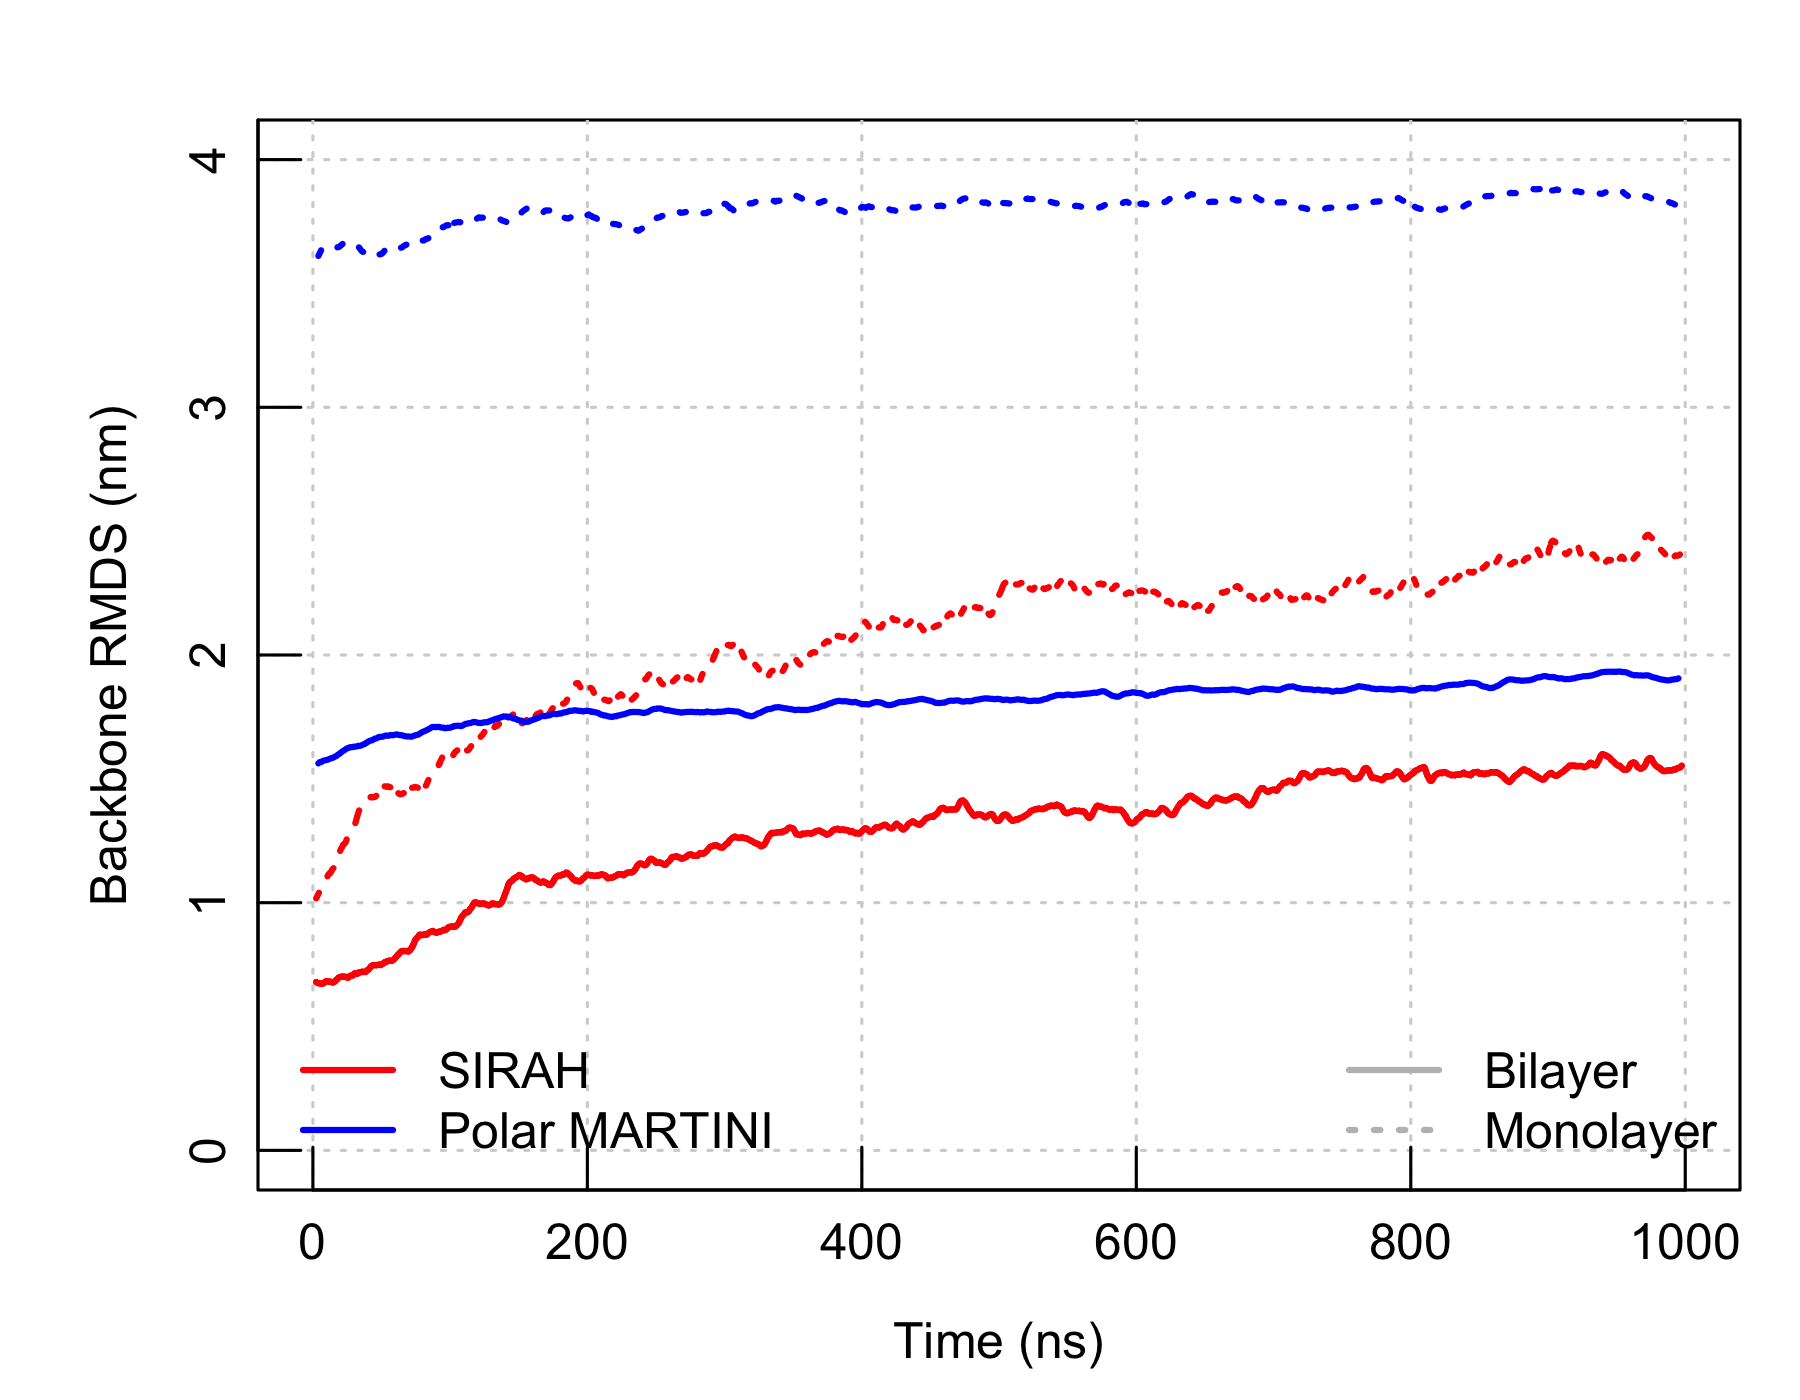
\includegraphics[width=0.48\linewidth, align=c]{3results_capsule/pics/compare_MonoBi_rmsd_init.png} \label{fig:rmsd_mono_bi}}
    \subbottom[]{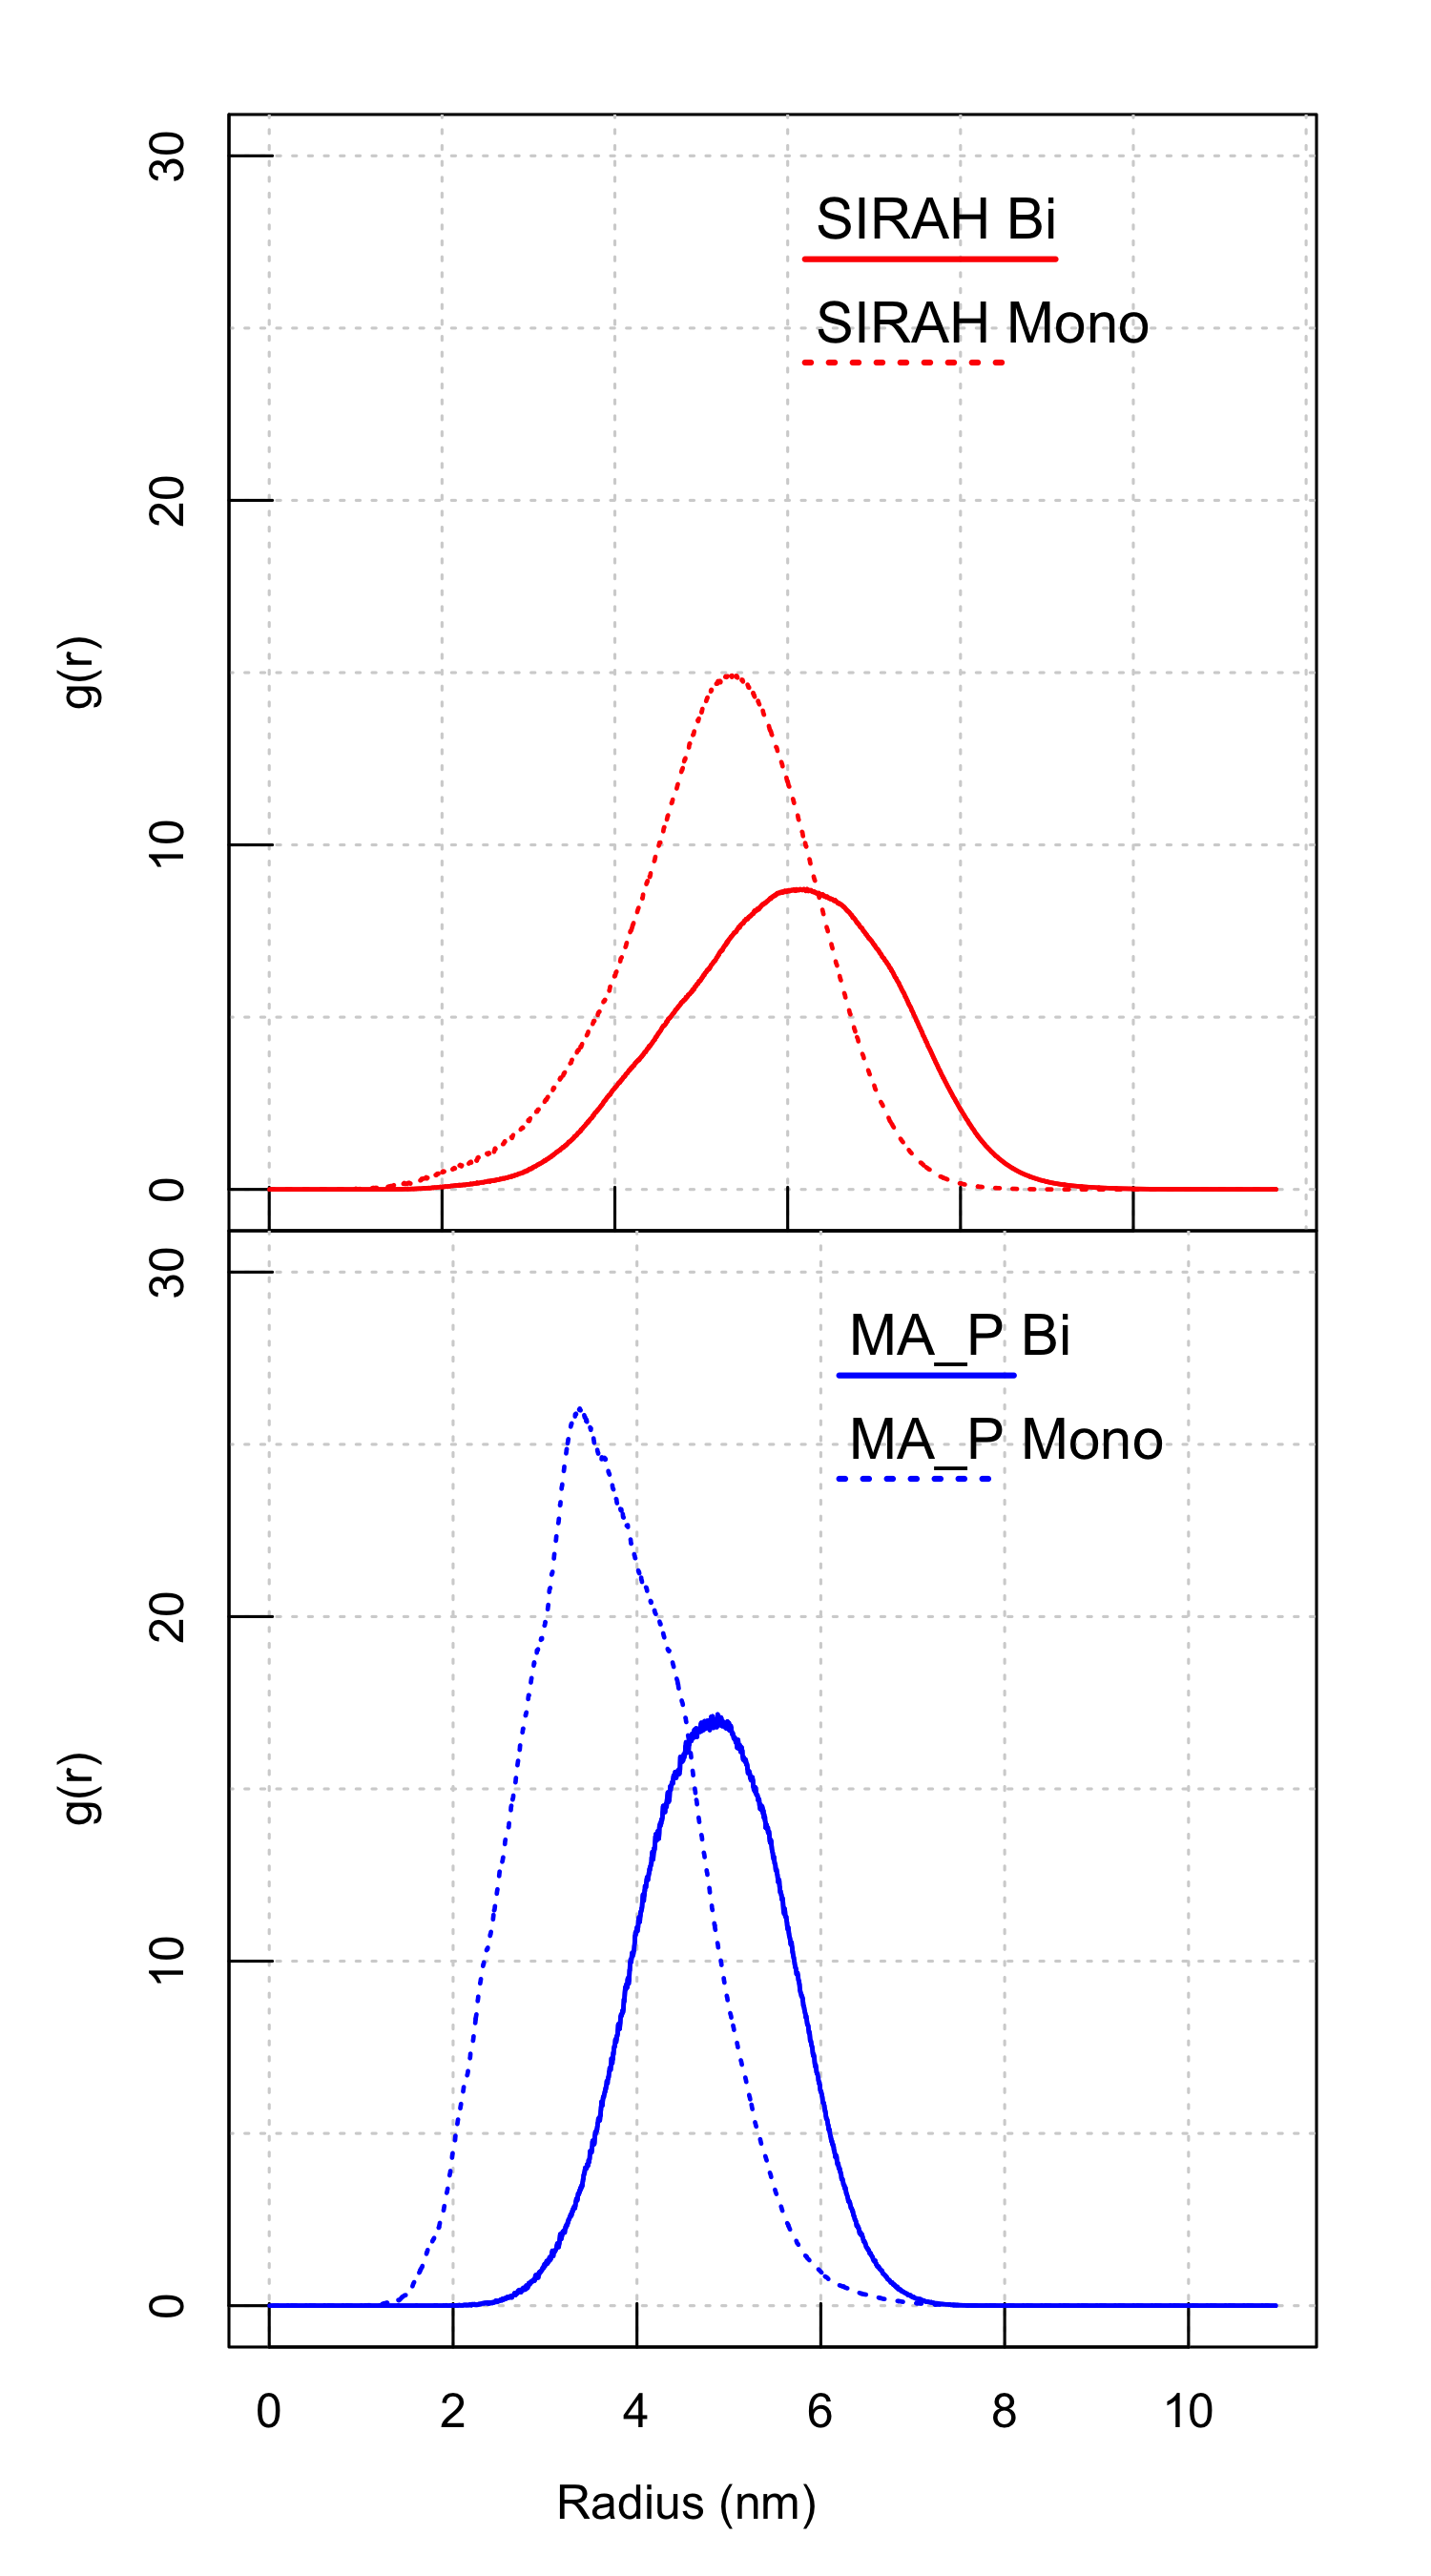
\includegraphics[width=0.48\linewidth, align=c]{3results_capsule/pics/compare_MonoBi_RDF.png} \label{fig:rdf_mono_bi}}
    \caption[Comparison of monolayer and bilayer structural properties]{(a) RMSD of the monolayer and bilayer structures for SIRAH and Polar MARTINI force fields, with respect to the initial geometrical configuration (external layer of Figure \ref{fig:BTI_vmd}, E). (b) RDF of Protein masses around their center of mass. For each label of the legend, the bar has length of the respective RDF FWHM (thickness estimate). Results are shown for Replica 1 of each simulation set-up.}
\label{fig:mono_bi}
\end{figure}

The RMSD with respect to the initially built structure (the geometrically regular polyhedra as in Figure \ref{fig:BTI_vmd}, E) shows that the monolayer undergoes a larger conformational change than the bilayer in the SIRAH force field and the effect is even more pronounced for the Polar MARTINI (Figure \ref{fig:rmsd_mono_bi}). 
%
As a note, we take as reference structure the regular geometry and not the first frame of the production as major rearrangements happen for the monolayer already in the equilibration phase, and those are different for each force field.
%
This larger change of the monolayer is due to a larger contraction of the structure, which collapses more toward its center (Figure \ref{fig:rdf_mono_bi}).

The SASA of each residue type computed on the initial configuration is slightly higher for the monolayer than the bilayer as expected, but this difference partially levels out during the simulations, due to the rearrangements mentioned above (Figure \ref{fig:mono_bi_sasa}). Therefore, coarse-grained representations suggest that the larger deformation observed in the monolayer is due mostly to the decrease in structural robustness when only one layer is present, and only in minor measure to the hydrophobic effect.
%
However the evidence collected through atomistic simulations of assembly of a few capzip molecules suggests the opposite - even if they can tackle a shorter time scale.
The atomistic simulation of a monolayer would be a useful piece of information to strengthen the conclusion derived, but was not run in the interest of time.

The discrepancy between coarse-grained and atomistic conclusions can be solved accepting both mechanisms (structural robustness and hydrophobic effect). Indeed, it is clear that coarse-grained descriptions have their weakest point in the ability of reproducing structural solvation, while they provide useful mechanical information.
 
Based on this, we deemed that the capsules observed experimentally must have a non-monolayer structure: a single layer would not provide enough structural stability and, moreover, it is not compatible with the thickness observed in the TEM images collected experimentally (Figure \ref{fig:afm_D}).

Overall, the multiscale investigation of this system provided information on how it is structured, but also a useful comparison between force fields, proving how the same system can be described in different ways from different models. This can be useful especially for the (comparatively) new SIRAH force field, which has been less assessed and less widely used than the MARTINI description.
%
\begin{figure}[t!]
\centering
\subbottom[]{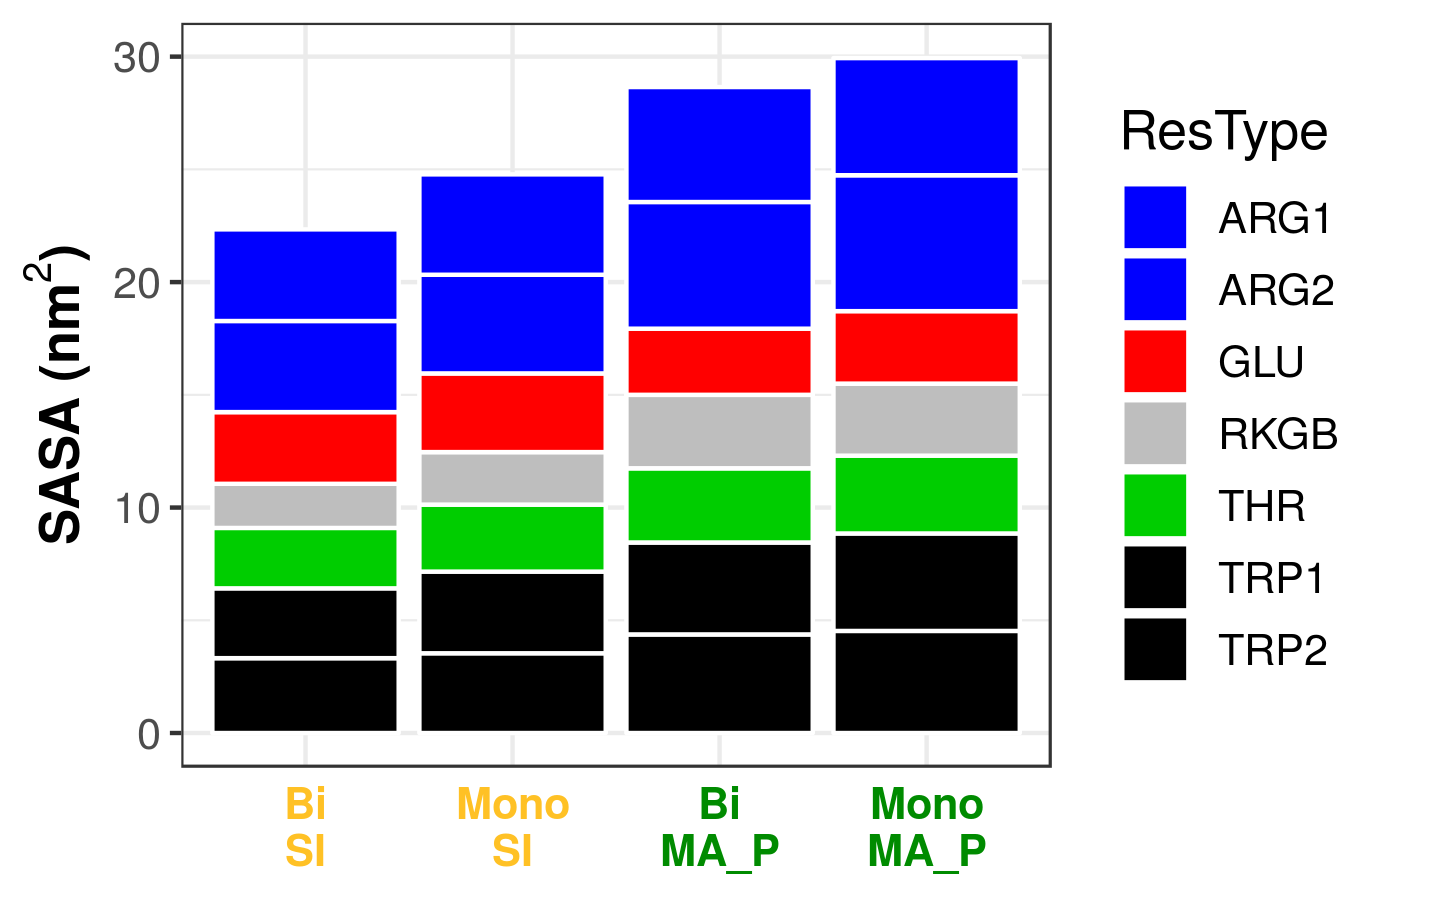
\includegraphics[width=0.48\linewidth]{3results_capsule/pics/st_sasaRes_mono_bi_init_bars.png} \label{fig:monobi_sasa_init}} 
\subbottom[]{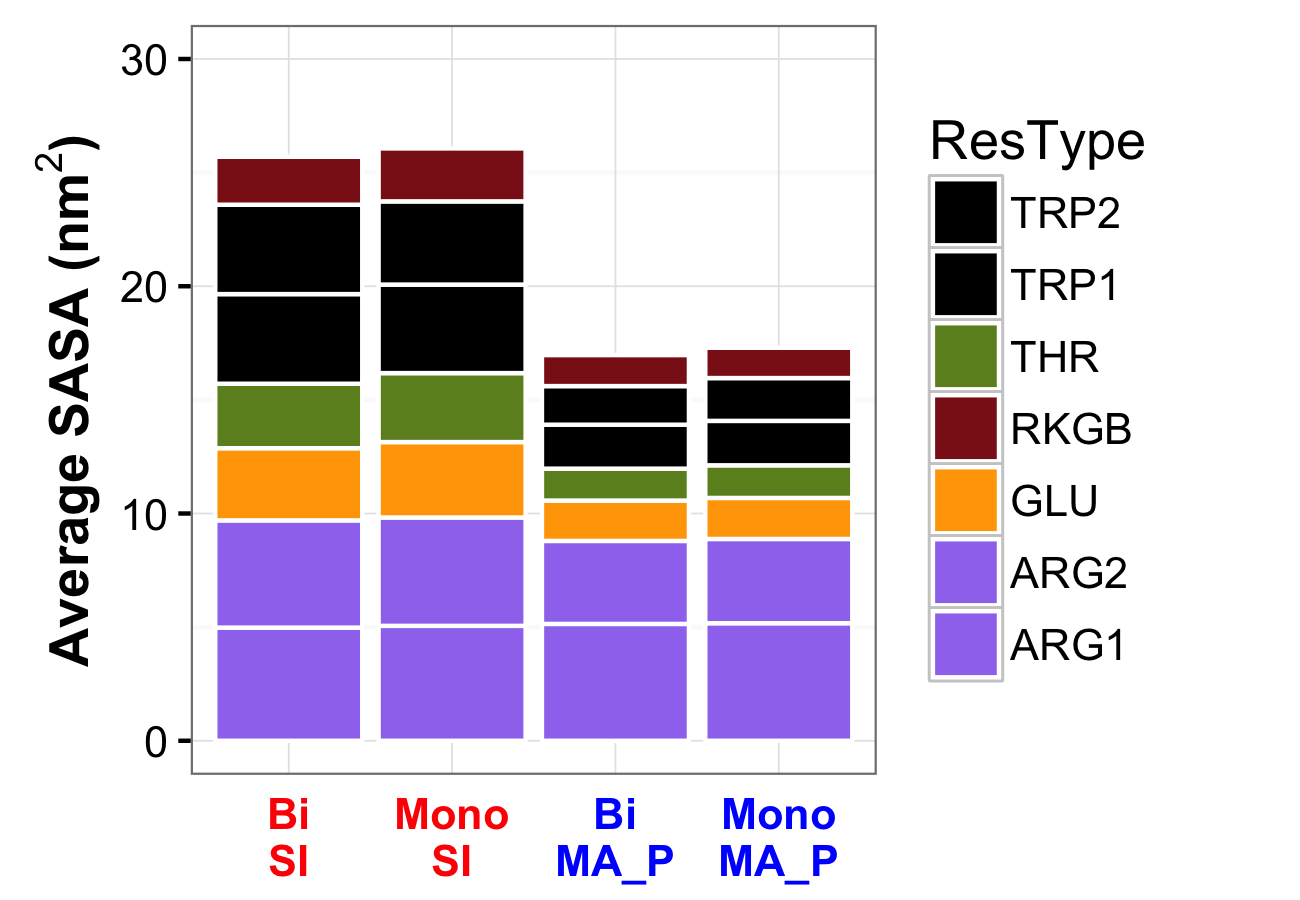
\includegraphics[width=0.48\linewidth]{3results_capsule/pics/st_sasaRes_mono_bi_bars.png} \label{fig:monobi_sasa_fin}} 
\caption[SASA per residue of monolayer and bilater]{Solvent Accessible Surface Area (SASA) per molecule, divided by residue types for simulations of the bilayer and monolayer structure. Results are shown for Replica 1 of each simulation set-up. (a) SASA computed from the initial configuration; (b) from the average over the production run.}
\label{fig:mono_bi_sasa}
\end{figure}


\subsection{Backmapped simulations} 

Two of the final configurations obtained from standard MARTINI simulations were backmapped to atomistic resolution, and simulated for additional 200 ns. The structures expanded roughly up to the sizes obtained in direct atomistic simulations (Figure \ref{fig:Rg_backmap}). They present however some unpaired arms and slightly deformed shapes, so that the RDF profiles of their masses around the origin results in a broader curve with respect to the original atomistic simulations, albeit they are centred at the same values (Figure \ref{fig:BM_RDF}).

The pattern of contacts per residue, computed on the last 100 ns of simulations, contains features of both the atomistic and MARTINI profiles (Figure \ref{fig:BM_contacts}).
%
\begin{figure}
\centering
\vspace{1cm}
\subbottom[]{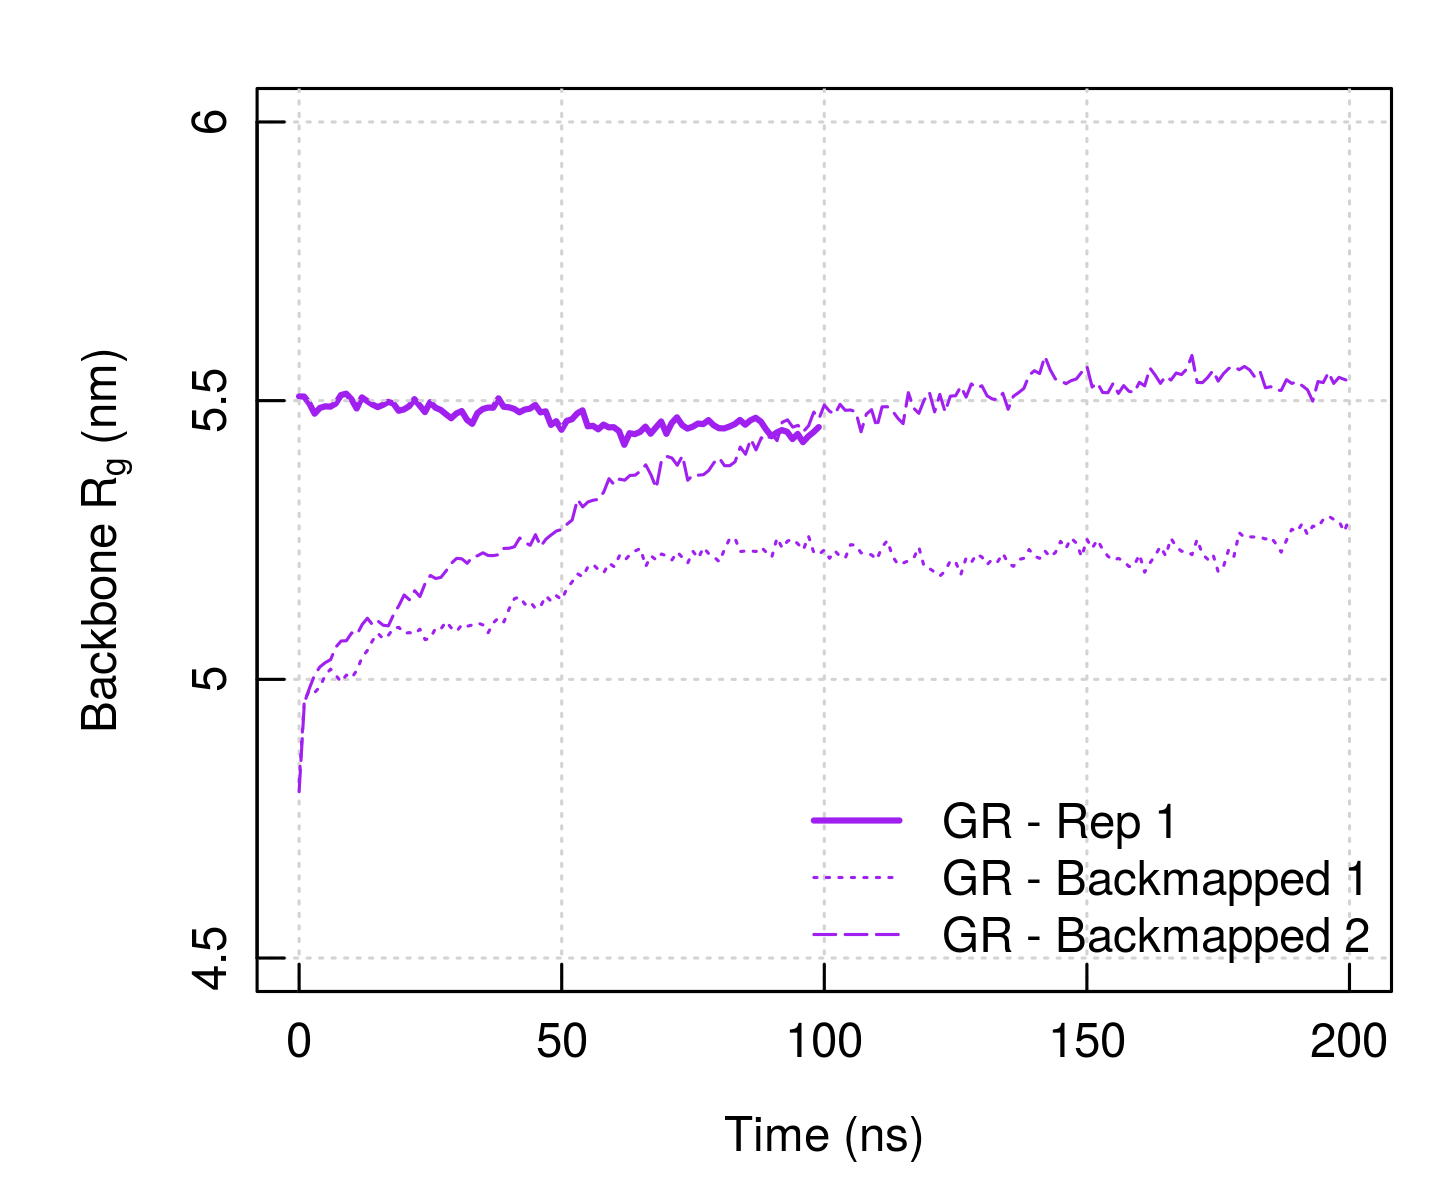
\includegraphics[width=0.48\linewidth]{3results_capsule/pics/Rg_backmap.png} \label{fig:Rg_backmap}}
\subbottom[]{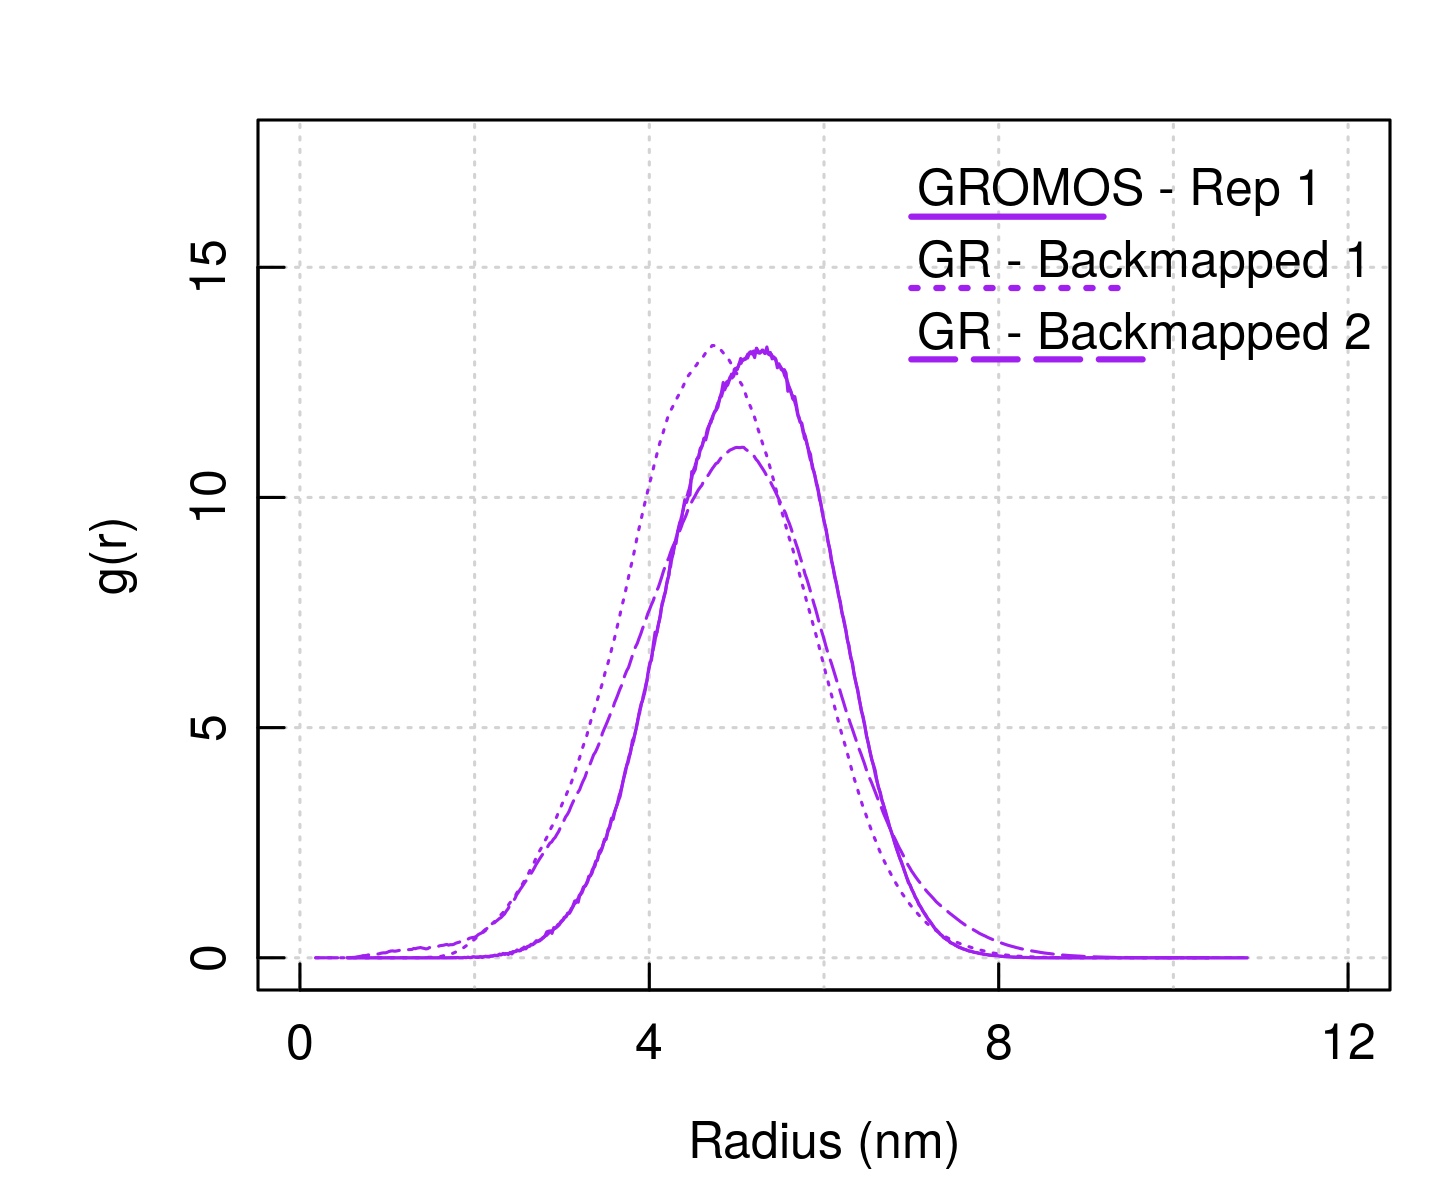
\includegraphics[width=0.48\linewidth]{3results_capsule/pics/RDF_BM.png} \label{fig:BM_RDF}}
\caption[Atomistic backmapped simulations: R$_g$ and RDF]{(a) Radius of gyration (computed on the protein backbone) and (b) RDF of protein masses around their centre for atomistic simulations (Replica 1) and backmapped atomistic from final configurations of Replica 1 and 2 of standard MARTINI runs. The RDF has been averaged over the last 50 ns of the original simulation, or 100 ns of the backmapped simulations. For each label of the legend in (b), the bar has length of the respective FWHM of the Gaussian function fitting the data (thickness estimate). }
\label{fig:backmap}
\vspace{1.5cm}
\centering
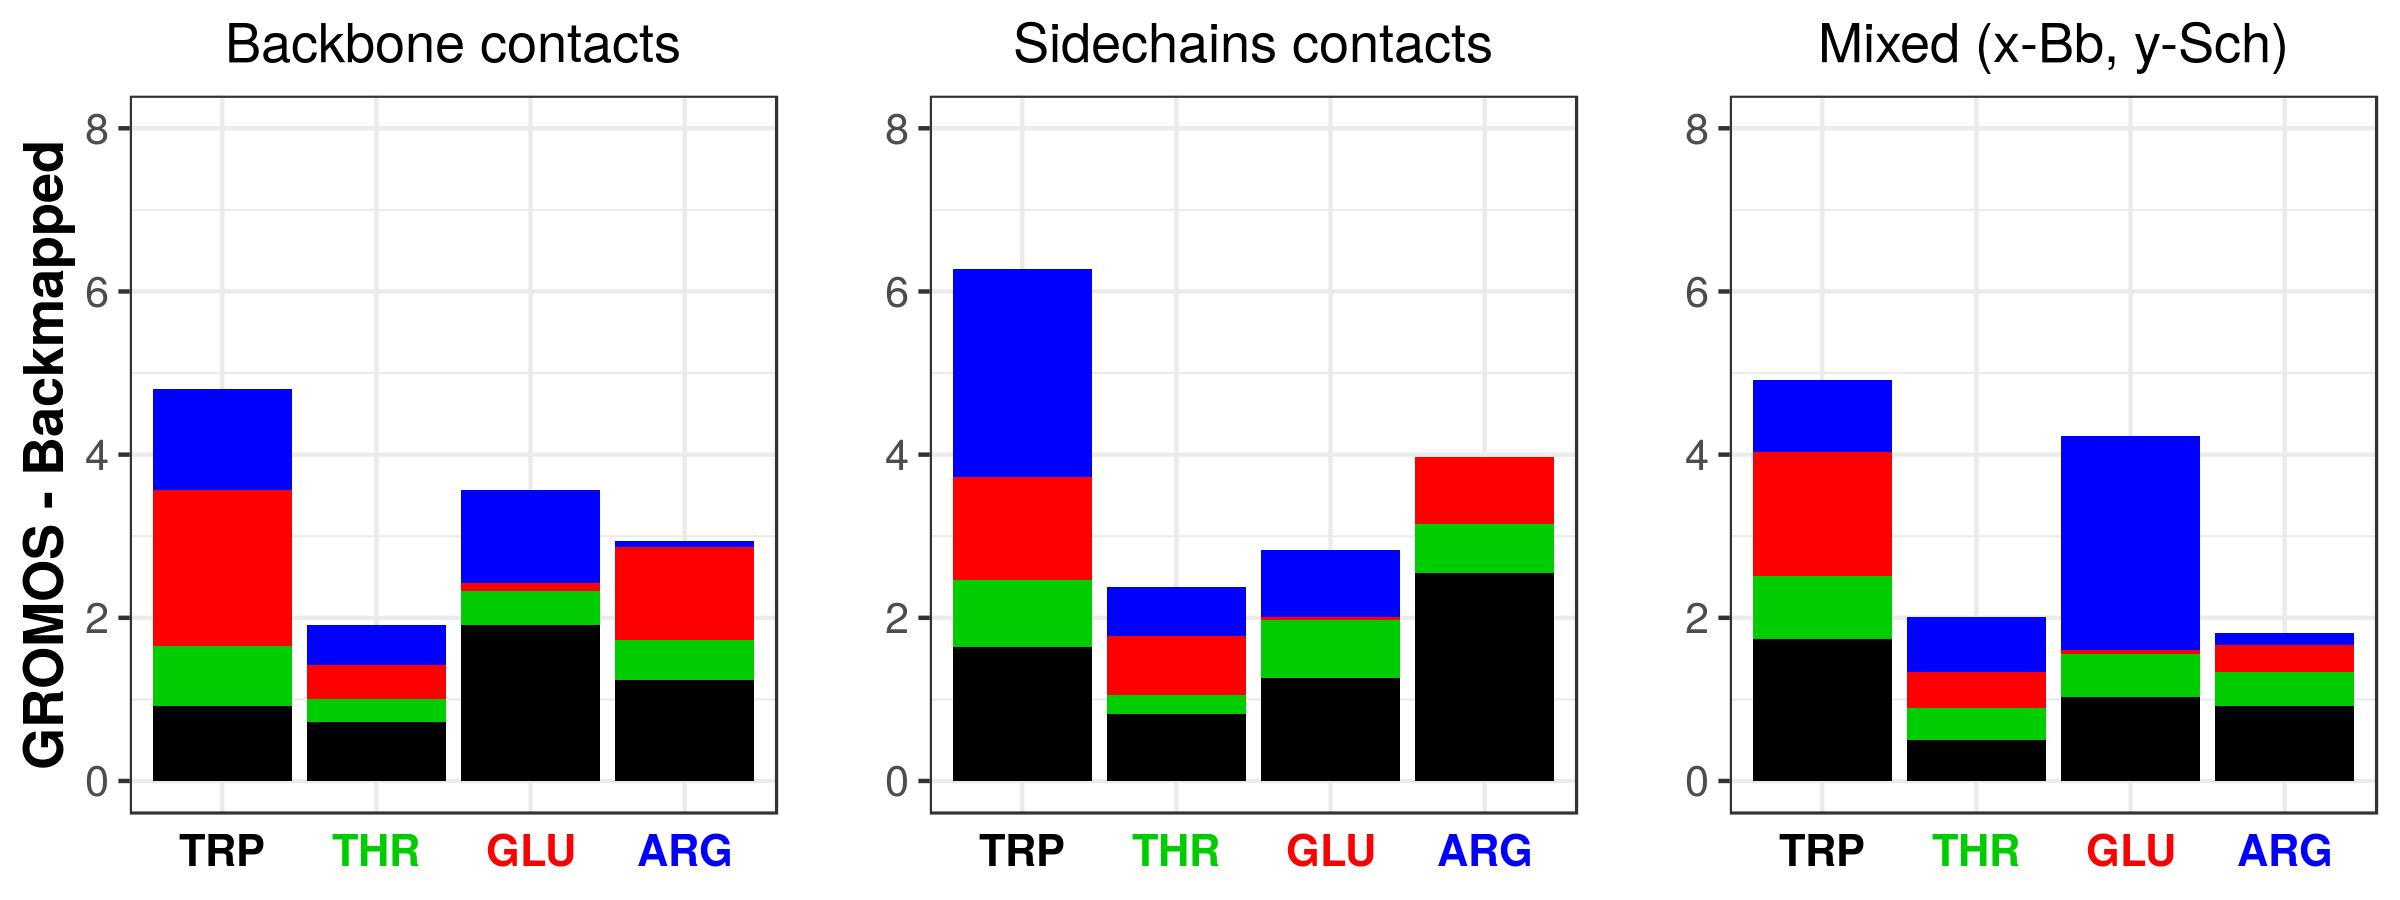
\includegraphics[width=0.95\linewidth]{3results_capsule/pics/contacts_BM.png} 
\caption[Atomistic backmapped simulations: contacts]{Number of contacts per residue type in each arm of capzip for an atomistic simulation backmapped from standard MARTINI (Replica 1): each bar shows the average number for the residue on the $x$-axis; its color is split by the identity of the partner residue (color coded as in the $x$-axis legend). For mixed contacts the residue on the $x$-axis contributes with its backbone. Results are shown for backmapped replica 1. Only contacts existing more than 50\% of the simulation time are considered.}
\label{fig:BM_contacts}
\vspace{1cm}
\end{figure}
%
In particular, at the side chain level, is recovered the interaction between Arginine and Tryptophan residues. Also for mixed backbone-side chain contacts the role of Tryoptophan with respect to the other residues is restored. For backbone contacts instead, the pattern resembles more the one from MARTINI. However, the number of total contacts is slightly lower, probably due to the rapid expansion which follows the backmapping procedure. This movement happens to relieve the unfavourable conformation deriving from the conversion between resolutions.

The expansion of the structure suggests that the atomistic simulations analysed before have indeed reached (or are reaching) an equilibrium: on one side, the atomistic radius of gyration in Figure \ref{fig:Rg} has not reached a plateau and could possibly decrease more, on the other, when the structure is contracted (as it is after the backmapping) it expands back to the larger size observed in Figure \ref{fig:Rg}. This suggest that the equilibrium value for an atomistic model lays between what found with an atomistic and a MARTINI coarse grain approach.


\clearpage
\section{Results: peptide-membrane interactions}

We now discuss simulations of capzip in contact with a membrane. First we focus on atomistic simulations of the pentagonal peptidic subunit in contact with a model bacterial or mammalian membrane, both under standard simulations conditions and with an applied external electric field. In this, we elucidate the local effect that the peptide has on the local lipid organisation.
%
We then analyse the process of membrane binding which is observed in coarse-grained simulations, comparing the MARTINI and Polar MARTINI force fields for the simulation without an external electric field, and necessarily resorting to Polar MARTINI for the ones involving it. 


\subsection{Atomistic simulations of the bacterial model membrane} \label{sec:lip_atom_bact}

Preliminary simulations were run on bacterial membranes alone (two lipid bilayers with 512 and 740 lipids respectively), to equilibrate them and compute their characteristics in absence of the peptide.
%
For the bacterial model chosen (DLPC/DLPG 3:1), we obtained an ApL of $0.580(5)$ nm$^2$ for the 512-lipid bilayer (simulated with GROMOS 54A7 force field), and  $0.569(4)$ nm$^2$ for the 740 one (GROMOS 54A8) as shown in Figure \ref{fig:lip_apl}, lines 1 and 5. No experimental values are available for this lipid mixture to compare the computational results.

\begin{sidewaysfigure}[p!]
\centering
\begin{minipage}{9.5cm}
\centering
\subbottom[]{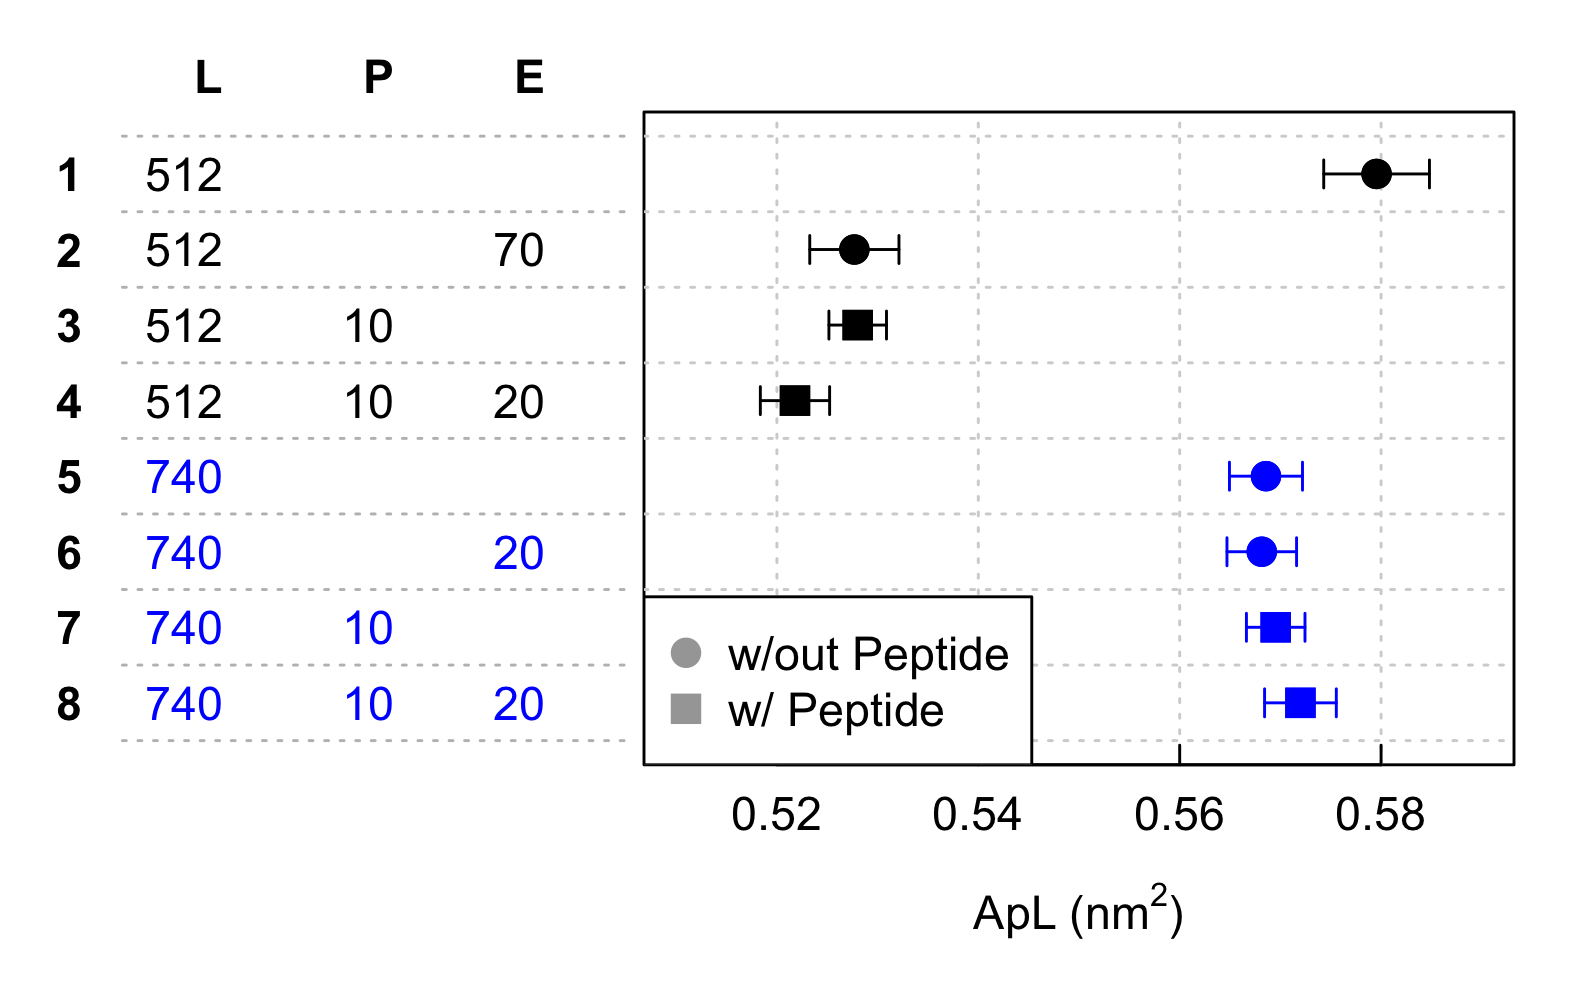
\includegraphics[height=6.3cm]{3results_capsule/pics/apl.png} \label{fig:lip_apl}} 
\end{minipage}
\begin{minipage}{5.6cm}
\centering
\subbottom[]{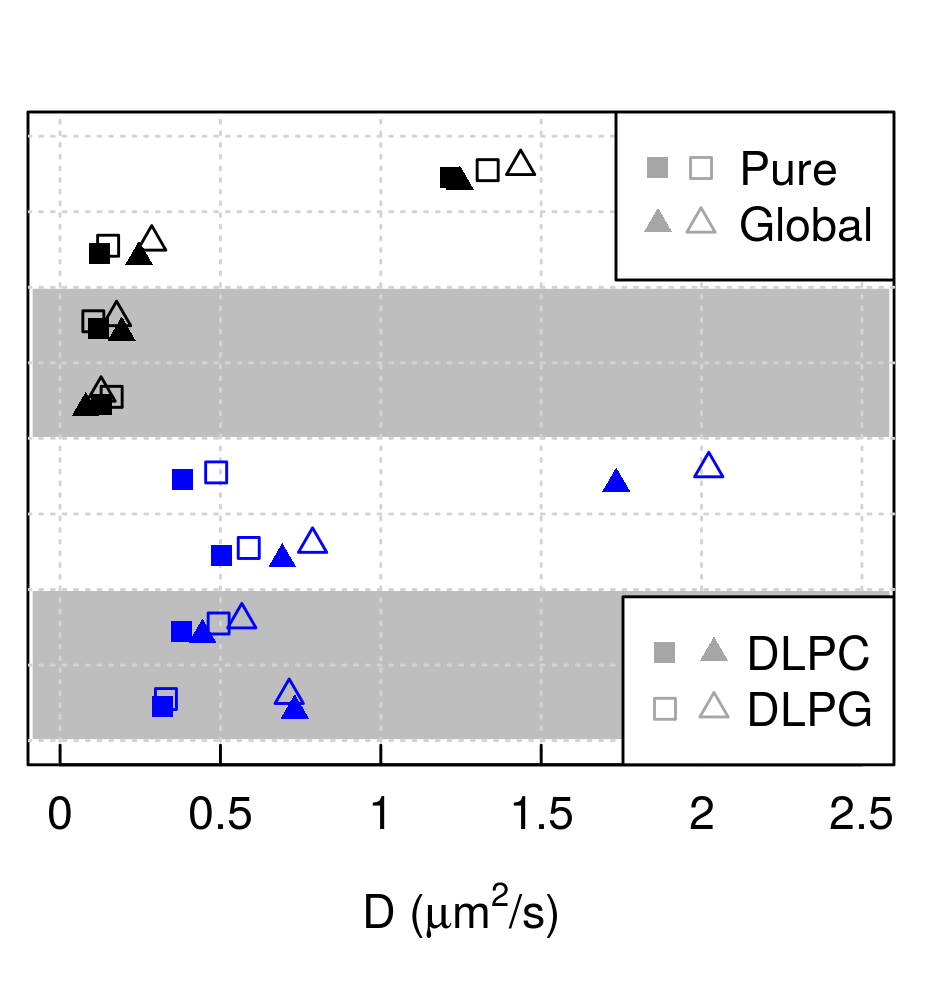
\includegraphics[height=6.3cm]{3results_capsule/pics/diff2_3.png} \label{fig:lip_diff}}
\end{minipage}
\begin{minipage}{5.6cm}
\centering
\subbottom[]{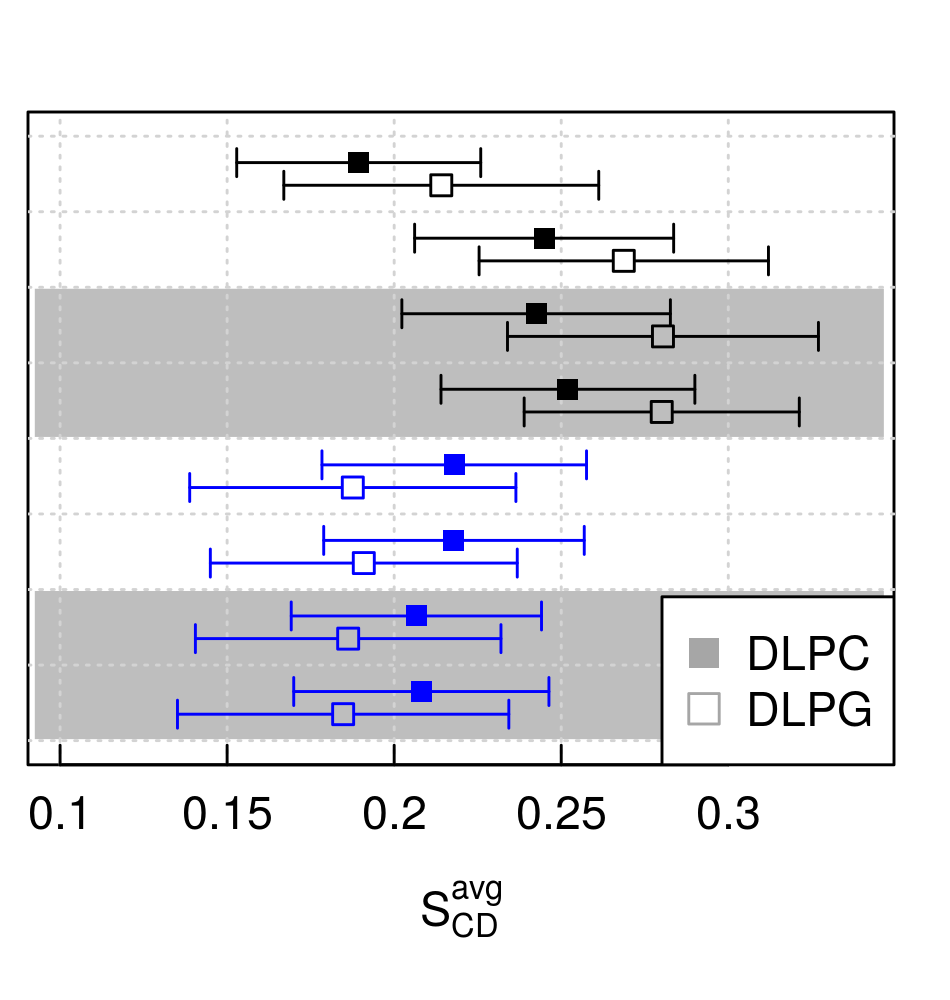
\includegraphics[height=6.3cm]{3results_capsule/pics/order2.png} \label{fig:lip_ord}} 
\end{minipage}
\caption[ApL, D and S$_{CD}$ for atomistic membrane simulations]{(a) Area per lipid (ApL); (b) pure and global lateral lipid diffusion coefficient (D), (c) average tail order S$^{avg}_{CD}$ from simulations of model bacterial membrane bilayers under different conditions. On the left of (a) a schematic of the system set-up shows the number of peptides P, number of lipids L, and electric field E applied in the z direction (in mV/nm) in each case. 
%
Black points refer to simulations on 512-lipid bilayers, blue ones on 740-lipid bilayers; shadowed regions flag systems where the peptide is present; in (b) squares refers to pure diffusion, triangles to global diffusion; in (b) and (c) full symbol are for DLPC, hollow ones for DLPG.
In (b) and (c) staggering along the $y$-axis helps the visualisation.
%
Bars denote the standard error; for the diffusion coefficients, these are smaller than the point size. Analysis performed discarding the first 200 ns of the simulations time.}
\label{fig:lipids_ApL_D}
\end{sidewaysfigure}

The difference is small but statistically significant (the two measures are not compatible within the error).
%
There are three differences between the two sets of simulations, and each of them can be responsible for the discrepancy.
First, the force field (GROMOS 54A7 versus 54A8, see Chapter \ref{chapter:lip_par} for a thorough comparison), then the long range electrostatic treatment (RF versus PME), and finally the size of the system (512 versus 740 lipids).
%
Regarding the first, extensive tests on phosphocholine lipids (see Chapter \ref{chapter:lip_par}) suggest that generally 54A8 gives larger ApL values than the ones computed with 54A7.
%
Regarding the second, a control simulation on the 512-lipid bilayer was run swapping the RF long range electrostatic treatment with PME (and maintaining the remaining set-up). It produced an ApL of 0.586(5), slightly larger that the one obtained with RF, but compatible with its value.
%
Therefore we attribute the discrepancy to the different sizes of the systems. Later in this section other cases are reported in which the size has a great influence on the simulation outcome.

Regarding the diffusion coefficient, we report in Figure \ref{fig:lip_diff} both the pure and global values (computed as explained in Section \ref{sec:analysis} and Figure \ref{fig:com_rem_scheme}).
%
Considering the pure diffusion (squares in Figure \ref{fig:lip_diff}), the larger membrane has a smaller coefficient with respect to the 512-lipid bilayer (line 1 and 5 of the Figure above). However, considering the global one (triangles) we observe the opposite.
%
In general, differences are expected between the two systems, because of their different size: it is well known that periodic boundary conditions affect the computed diffusion coefficient D \citep{Camley2015,Venable2017}. Previous studies found that, for atomistic simulations of the size employed here, D is systematically underestimated \citep{Camley2015}: increasing the size would increase the coefficient, toward its real value (which is obtained for an infinite box). This is consistent with our global diffusion results, but not the pure ones. Unfortunately, it is not clear whether, in the publications mentioned, they refer to what is here defined as pure or global diffusion.

To exclude that the difference between the two systems is given by the force field chosen, we refer the reader to the next chapter, where, for simulations of monolipid bilayers, the 54A7 or 54A8 force fields gave very similar values of pure diffusion, keeping all the other simulations conditions identical (of the order of 0.1 $\mu$m$^2$/s).
%
Also in those simulations we observed drift of one leaflet with respect to the other, which would produce discrepancy between the values of pure and global D. The drift appeared in some of the simulations only, and not in a consistent manner: it did not happen for a lipid in particular, nor for a specific set of parameters. This suggests that small changes in the the initial conditions can lead to very different values of the drift (if any exist).
However, once it is started, such motion seems to persist throughout the simulation length, consistently with the inertia gained by the leaflet.


\paragraph{Interaction of the peptide with the 512-lipid model bacterial membrane}
For the small bilayer, the presence of the pentagonal peptide subunit (made of ten antimicrobial molecules, and bearing a $+60\,e$ total charge) made the ApL decrease by 9\% with respect to the value of the membrane itself (Figure \ref{fig:lip_apl}, line 3 versus 1).
%
A similar effect was observed applying an electric field of 70 mV/nm intensity or combining the peptide with a 20 mV/nm field, comparable with physiological values (Figure \ref{fig:lip_apl}, lines 2 and 4).
%
Given the high net charge of capzip, the molecule itself produces an electric field, thus the perturbation on the membrane is similar to the one obtained when the field is externally applied.

The fact that both the peptide and/or the electric field lead to reduction of ApL of a similar amount suggests that the membrane is approaching the maximum packing allowed.
%
Consistently, the diffusion coefficients had a 6-fold reduction for both species of lipids (Figure \ref{fig:lip_diff}). Pure and global diffusion are very similar, as there is little translation between the leaflets.
%
At the same time, the order parameter S$^{avg}_{CD}$ increased slightly (Figure \ref{fig:lip_ord}). The variability on S$^{avg}_{CD}$ is high, showing that some regions reached a value larger than 0.3, which is often associated to transition to the gel phase, characterised by highly order lipid chains \citep{Pluhackova2016}.
%
To investigate this, for the simulation in presence of capzip, the hexagonal order parameter $S_6$ is computed for the bottom leaflet of the membrane (the one not hosting the pentagonal subunit, if present). This shows a few lipids in the gel phase, i.e.\ S$_6 \ge 0.72$ (Figure \ref{fig:S6_pb4}): despite there is no formation of ordered clusters, the shrinking of the membrane due to the presence of capzip increases the lateral order (and the thickness of the membrane). Indeed no lipid reaches the S$_6$ gel threshold in the simulations of a pure membrane (data not shown).
%
\begin{figure}
\centering
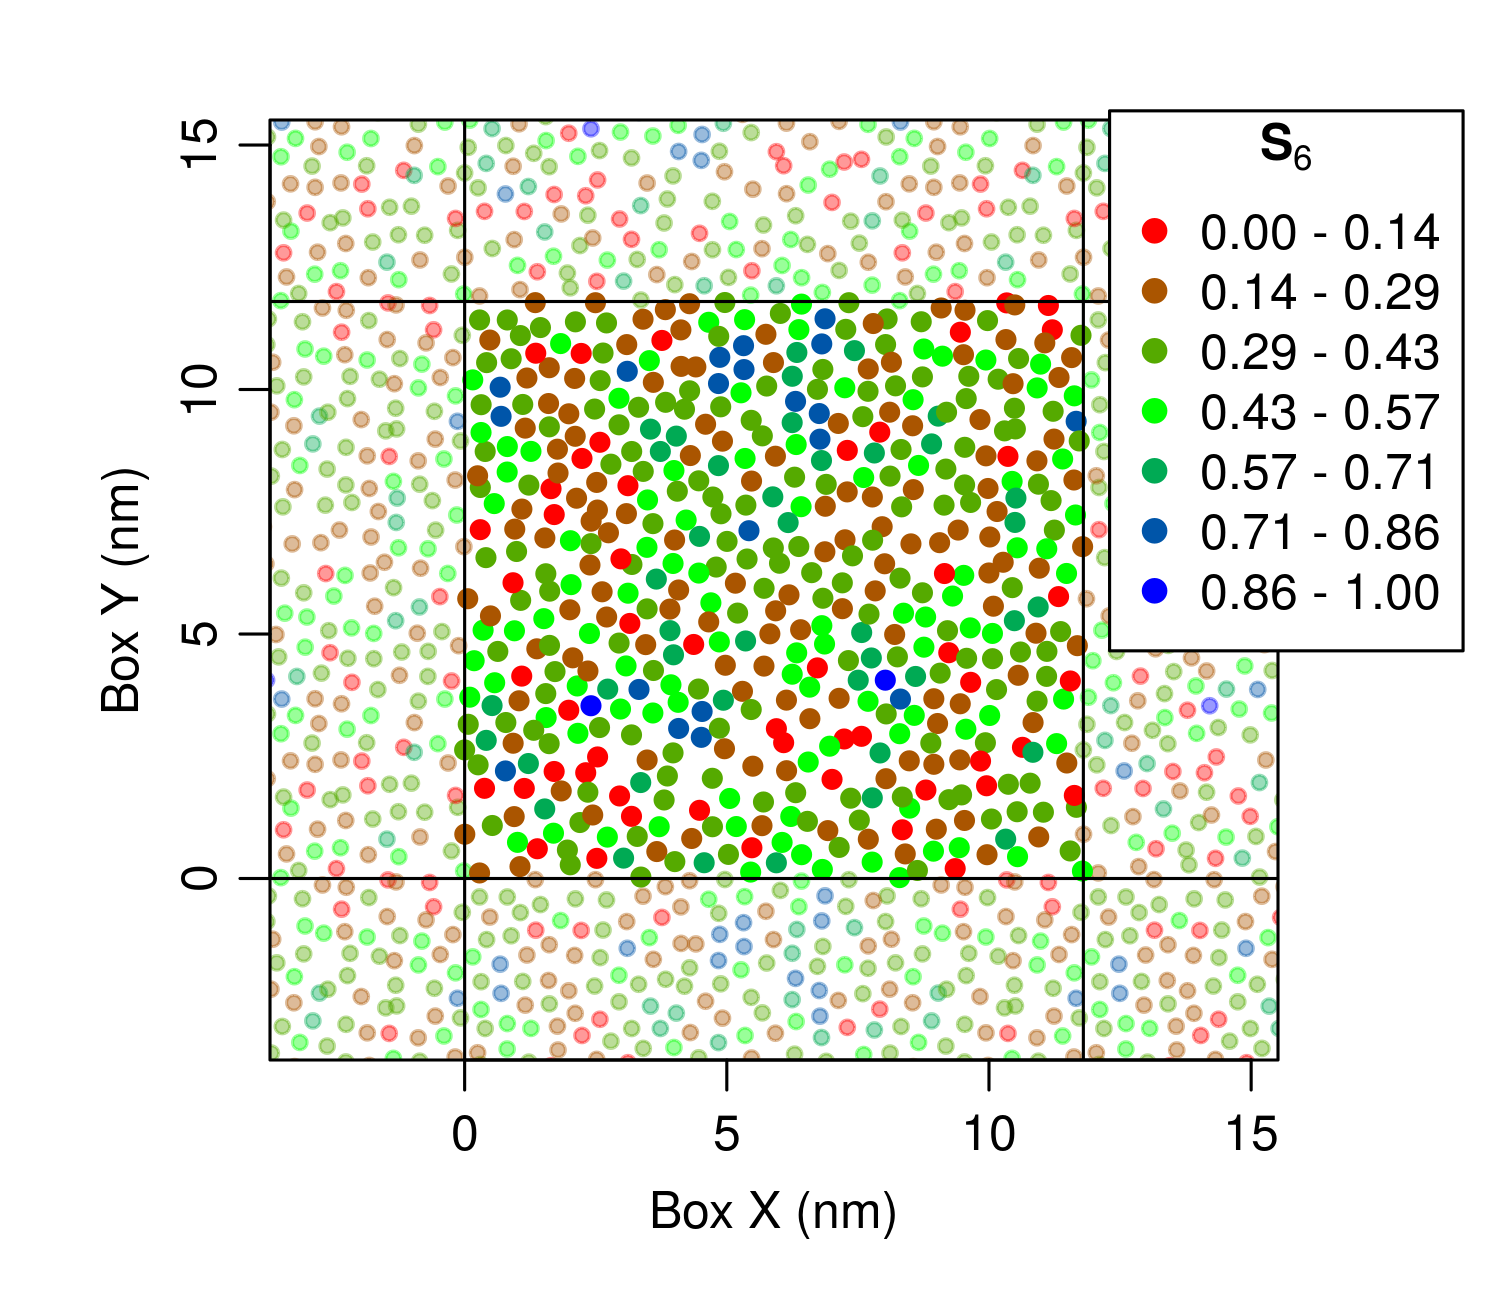
\includegraphics[width=0.5\linewidth]{3results_capsule/pics/pb4_S6.png} 
\caption[Lipid hexagonal order parameter in an atomistic protein-lipid simulation]{Hexagonal order parameter S$_6$ for the bottom leaflet lipid acyl chains, computed on the last frame of a simulation of a 512-lipid bacterial bilayer with 10 peptide molecules (line 3 in \ref{fig:lipids_ApL_D}). Chains plotted by the average $xy$ position of their carbon atoms, and colour coded by the S$_6$ value; chains of the periodic images shown faded out; boundaries of the simulation box in solid black lines.}
\label{fig:S6_pb4}
\end{figure}

\paragraph{Interaction of the peptide with the 740-lipid model bacterial membrane}

When we simulated the 740-lipid bilayer with an externally applied electric field and/or in presence of the peptide, the ApL and tail order parameter S$^{avg}_{CD}$ remained equal, within the error, to the values obtained from simulations of the membrane alone.

The global diffusion coefficient D was still significantly affected, being reduced between 2.5 and 5 times (Figure \ref{fig:lipids_ApL_D}, lines 5 to 8), but not the pure diffusion. The simulation of the 740-lipid bacterial membrane alone is the only case, among all the simulations results shown in Figure \ref{fig:lip_diff}, in which pure and global D differ substantially. However, as commented above, the leaflet translation seems to be dependent on the initial conditions, thus we can not be certain that this translation is a consistently reproducible effect.

While, for the small bilayer, perturbations reduced the diffusion and the ApL together, the results on the larger membrane show that neither ApL nor pure diffusion are affected from the peptide/electric field.
%
However, given the decrease in global diffusion, an the fact that the peptide is likely to influence the movement of the lipids nearby itself, we computed the diffusion coefficient for subsets of lipids based on their distance from the peptide at the initial frame of the production run (Table \ref{table:D_space}). On this occasion, the trajectory was centred around the peptide COM, to understand the lipid movement with respect to it. The lipids closer to the protein resulted indeed the most slowed down in their motion. DLPG is slightly more mobile than DLPC, as observed in all the 740-lipid bilayer simulations (Figure \ref{fig:lip_diff}).

%
\begin{figure}[p!]
\centering
 \def\arraystretch{1.6}
\begin{tabular}{lllllll}
\multicolumn{7}{c}{\textbf{Local diffusion for DLPC/DLPG with capzip}} \\
\hline
& & & \multicolumn{2}{c}{\textbf{DLPC}} & \multicolumn{2}{c}{\textbf{DLPG}} \\
 \hline
Lip. & Pept. & Region & Nr. & D ($\mu m^2/s$) & Nr. & D ($\mu m^2/s$) \\
 \hline
10 & 737 & $d<1$ & 93 & 0.283(1) & 38 & 0.272(2)  \\
10 & 737 & $d<2$ & 152 & 0.325(2) & 52 & 0.353(3) \\
10 & 737 & $d<3$ & 239 & 0.402(2) & 70 & 0.393(3) \\
10 & 737 & $d>3$ & 329 & 0.442(3) & 98 & 0.650(4) \\
10 & 737 & All & 568 & 0.486(3) & 169 & 0.541(3) \\
 \hline
0 & 740 & All (global) & 570 & 1.75(3) & 170 & 2.02(2) \\
0 & 740 & All (pure) & 570 & 0.383(1) & 170 & 0.487(3) \\
 \hline
 \end{tabular}
\captionof{table}[Local diffusion coefficient for DLPC/DLPG with capzip (atomistic)]{Local diffusion for the DLPC/DLPC bilayer in presence of capzip. 
%
Pept.: number of peptides; Lip.: number of lipids.
%
The values are computed for groups of lipids which, at the initial time, are at a distance $d$ smaller than 1 nm, 2 nm or 3 nm from the peptide or larger than 3 nm (Regions).
%
D is computed centring the trajectory around the Protein COM. The pure and global diffusion coefficients for the pure membrane are given for comparison. Error from linear fit in parenthesis.}
\label{table:D_space}

\vspace{0.5cm}

\centering
 \def\arraystretch{1.6}
\begin{tabular}{lcccccccccc}
\multicolumn{11}{c}{\textbf{Capzip - DLPC/DLPG lipids hydrogen bonds}} \\
\hline
&& \multicolumn{4}{c}{\textbf{E = 0 mV/nm}} && \multicolumn{4}{c}{\textbf{E = 20 mV/nm}} \\
\hline
 && \multicolumn{2}{c}{Total} & \multicolumn{2}{c}{$\displaystyle\tau \ge 50$\%}  && \multicolumn{2}{c}{Total} & \multicolumn{2}{c}{$\displaystyle\tau \ge 50$\%} \\
\hline
  && \multicolumn{1}{c}{R} & \multicolumn{1}{c}{W} & \multicolumn{1}{c}{R} & \multicolumn{1}{c}{W} && \multicolumn{1}{c}{R} & \multicolumn{1}{c}{W} & \multicolumn{1}{c}{R} & \multicolumn{1}{c}{W} \\
% \hline
 {DLPC} && 668 & 73 & 20 & 7 && 798 & 90 & 18 & 6 \\
 {DLPG} && 928 & 114 & 12 & 3 && 980 & 104 & 16 & 3 \\
 \hline
 {All} && \multicolumn{2}{c}{2041} & \multicolumn{2}{c}{50} && \multicolumn{2}{c}{2238} & \multicolumn{2}{c}{54} \\
\hline
 \end{tabular}
\captionof{table}[Hydrogen bonds between capzip and DLPC/DLPG (atomistic)]{Number of hydrogen bonds between the Arginine (R) or Tryptophan (W) residues of the pentagonal subunit (10 capzip molecules) and DLPC or DLPG lipids (740-lipid bacterial bilayer). Results shown for simulations without electric field (left) or a 20 mV/nm field (right).
%
The table displays both the total number of observed hydrogen bonds (Total) and the ones present for more than 50\% of the simulated time, not necessarily in a continuous fashion ($\displaystyle\tau \ge 50$). Furthermore, the corresponding figures for all the bonds occurring between any residue of the peptide and any lipid is displayed (All).}
\label{table:hb_pr_lip}
\end{figure}

The local slowing down of lipids is due to electrostatic and hydrogen bond interactions between the lipids and the peptide. We computed the latter, monitoring the ones which persisted more than 50\% of the time, not necessarily i n a continuous fashion (Table \ref{table:hb_pr_lip}). Moreover, we singled out the ones involving Arginine and Tryptophan residues.
%
Arginine promotes many persistent bonds, and the number of them is equally divided between DLPC and DLPG residues, despite there are less DLPG residues overall. Tryptophan promotes fewer persistent bonds; and the remaining ones that exist for more than 50\% of the time involve all Threonine residues.
%
Thus, hydrogen bonds, together with the electrostatic attraction between positive residues of the peptide and negatively charged DLPG lipids, slow down the dynamics of the lipids close to the peptide, which do not diffuse away. The presence of a less mobile patch of lipids influences the diffusion of the ones nearby as well, decreasing it.

Regarding the position of the amino acid within the lipid membrane, Figure \ref{fig:aa_insertion_bact} shows a plot of the average insertion during the last 100 ns of the simulation. This is computed taking into account for each amino acid the atom with the lowest $z$ coordinate, which is compared with the maximum $z$ coordinates of the lipids around it. In this way, the local height of the membrane is taken into account. The results show a deeper insertion of Arginine residues on average, while Tryptophan inserts less, and some of them are placed at the interface with solution. This will be important for the initiation of pores in simulations with an external electric field (see the next paragraph).
%
\begin{figure}[t!]
\centering
\subbottom[]{
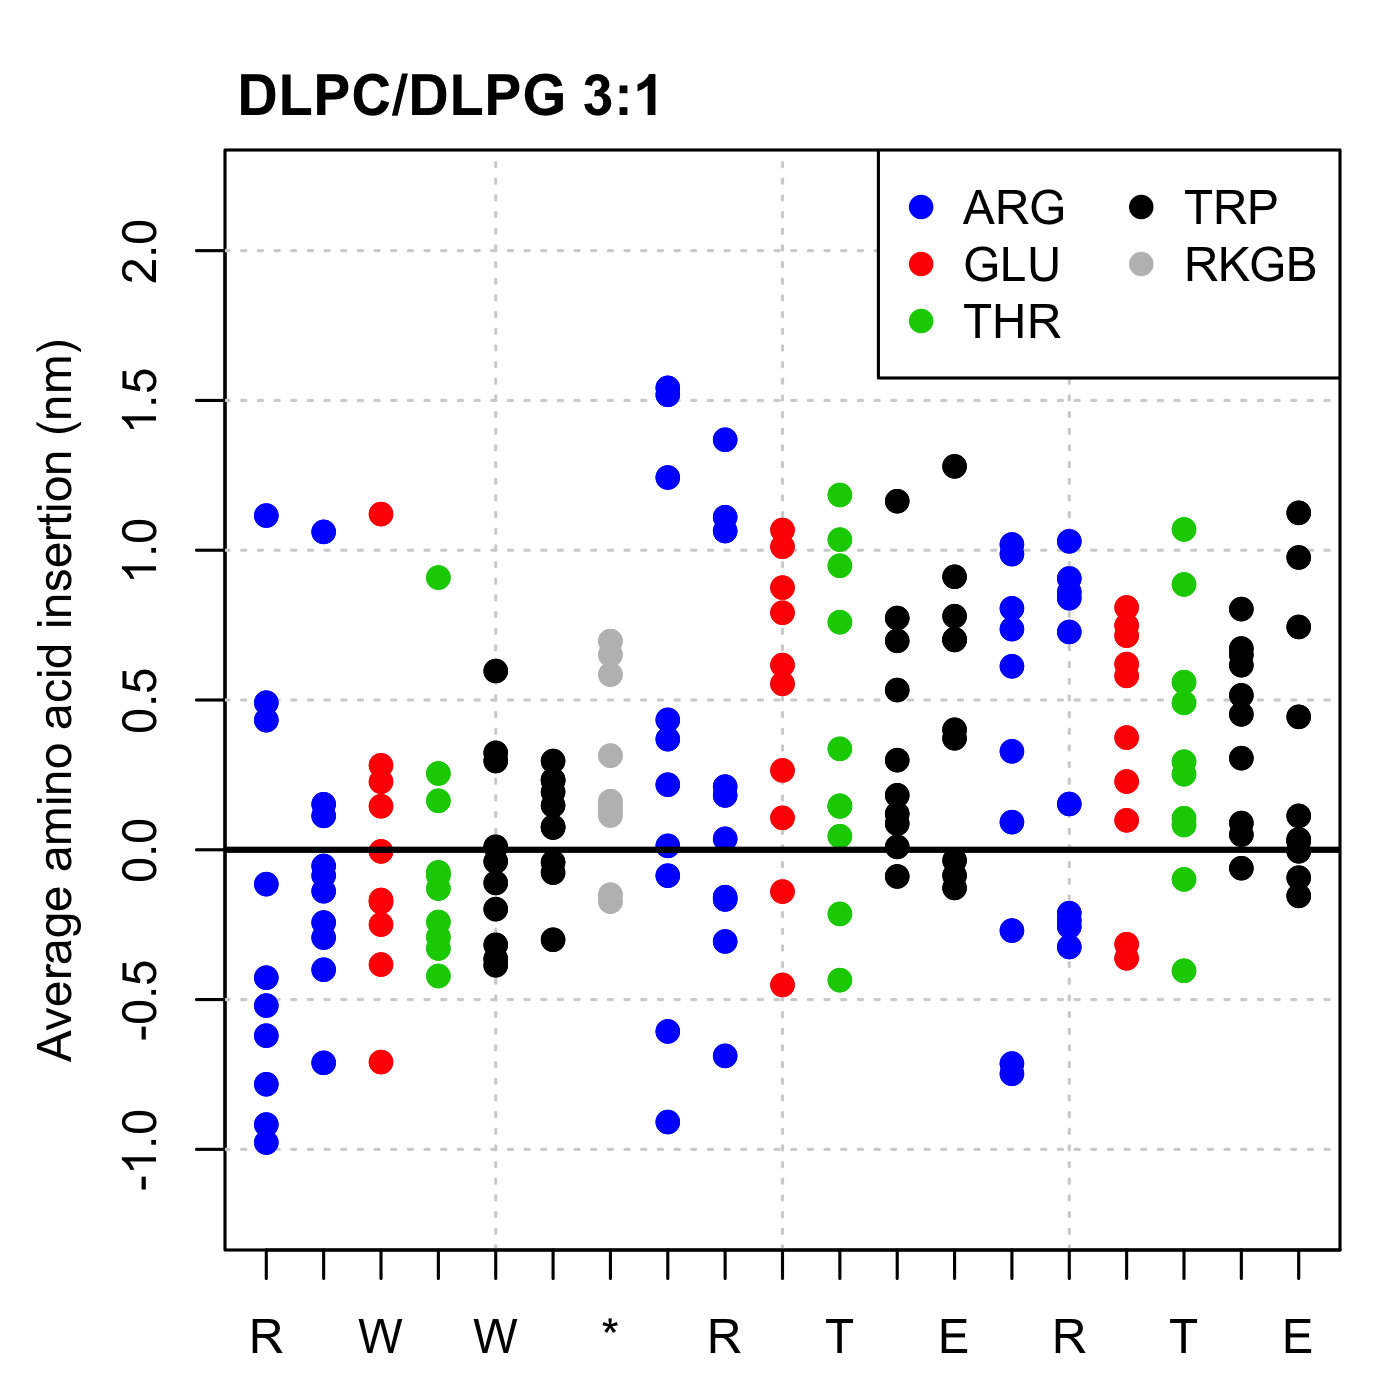
\includegraphics[width=0.47\linewidth]{3results_capsule/pics/pL6_avg_depth_mix.png} \label{fig:aa_insertion_bact}}
\subbottom[]{
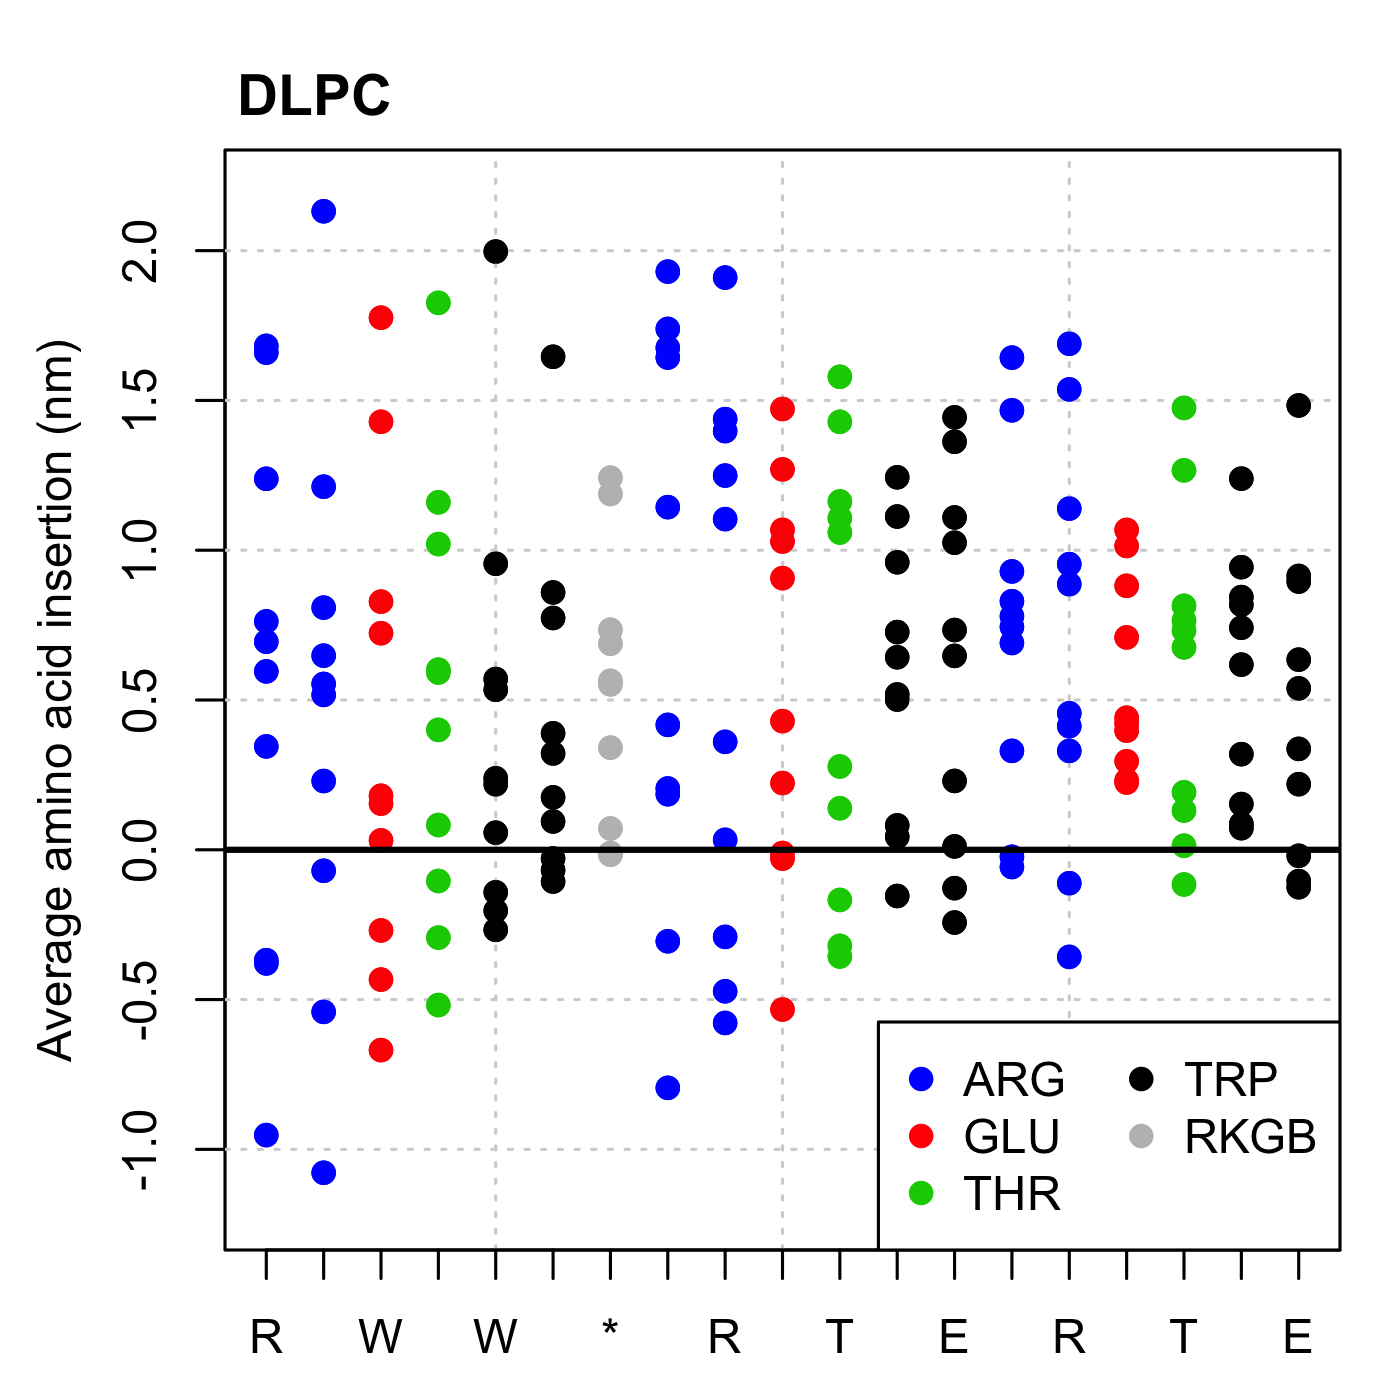
\includegraphics[width=0.47\linewidth]{3results_capsule/pics/pZ11_avg_depth_mix.png} \label{fig:aa_insertion_mamm}}
\caption[Insertion of capzip amino acid in model membranes (atomistic)]{Insertion of each amino acid of the pentagonal subunit within a bacterial (a) or mammal (b) model membrane. The $x$-axis shows the amino acids in the capzip sequence, with $\cdot$ indicating the RKGB central residue (19 overall). The boxes shows the range on the 10 molecules forming the pentagonal subunit.}
\label{fig:aa_insertion}
\end{figure}

We think that this reduced ``fluidity" in terms of lateral diffusion is an important perturbation of the membrane structure, as it diminishes its ability to accommodate external stimuli, such as water penetration. With coarse-grained simulations (see Section \ref{sec:results_lip_cg}) it will be evident that on the long time scale, these interactions are also able to recruit anionic lipids around the peptide, creating a local imbalance in the membrane composition.


\paragraph{Electroporation results}
As it is not possible to witness the penetration of the peptide through the membrane within the available simulation time, we opted to perform electroporation simulations.
%
An electric field of increasing intensity was applied along the negative $z$ direction perpendicular to the membrane, with the peptide on the positive $z$ side, to model the field generated by the transmembrane potential.

The field was increased of 20 mV/nm every 200 ns (or 10 mV/nm when approaching the poration threshold). The initial value of 20 mV/nm was chosen as it is an approximation of the physiological value of the transmembrane potential (see discussion in Section \ref{sec:details}). This procedure showed that the critical value of 130 mV/nm triggered poration in the presence of the peptide. 
%
This was confirmed by three replicas run with a 130 mV/nm field from the initial unperturbed membrane configuration (poration after 20 ns, 75 ns and 71 ns respectively).
%
Similarly, on the 740-lipid bilayer in presence of capzip, the same field induced membrane disruption after 60 ns, 50 ns and 70 ns respectively (Figure \ref{fig:pore_pics_2}).
%
This value is significant at the time scale used, and it is possible that for longer time scales one can witness poration at lower values of the electric field.

\begin{figure}[t!]
\centering
\begin{minipage}[b]{0.26\linewidth}
\centering
\subbottom[]{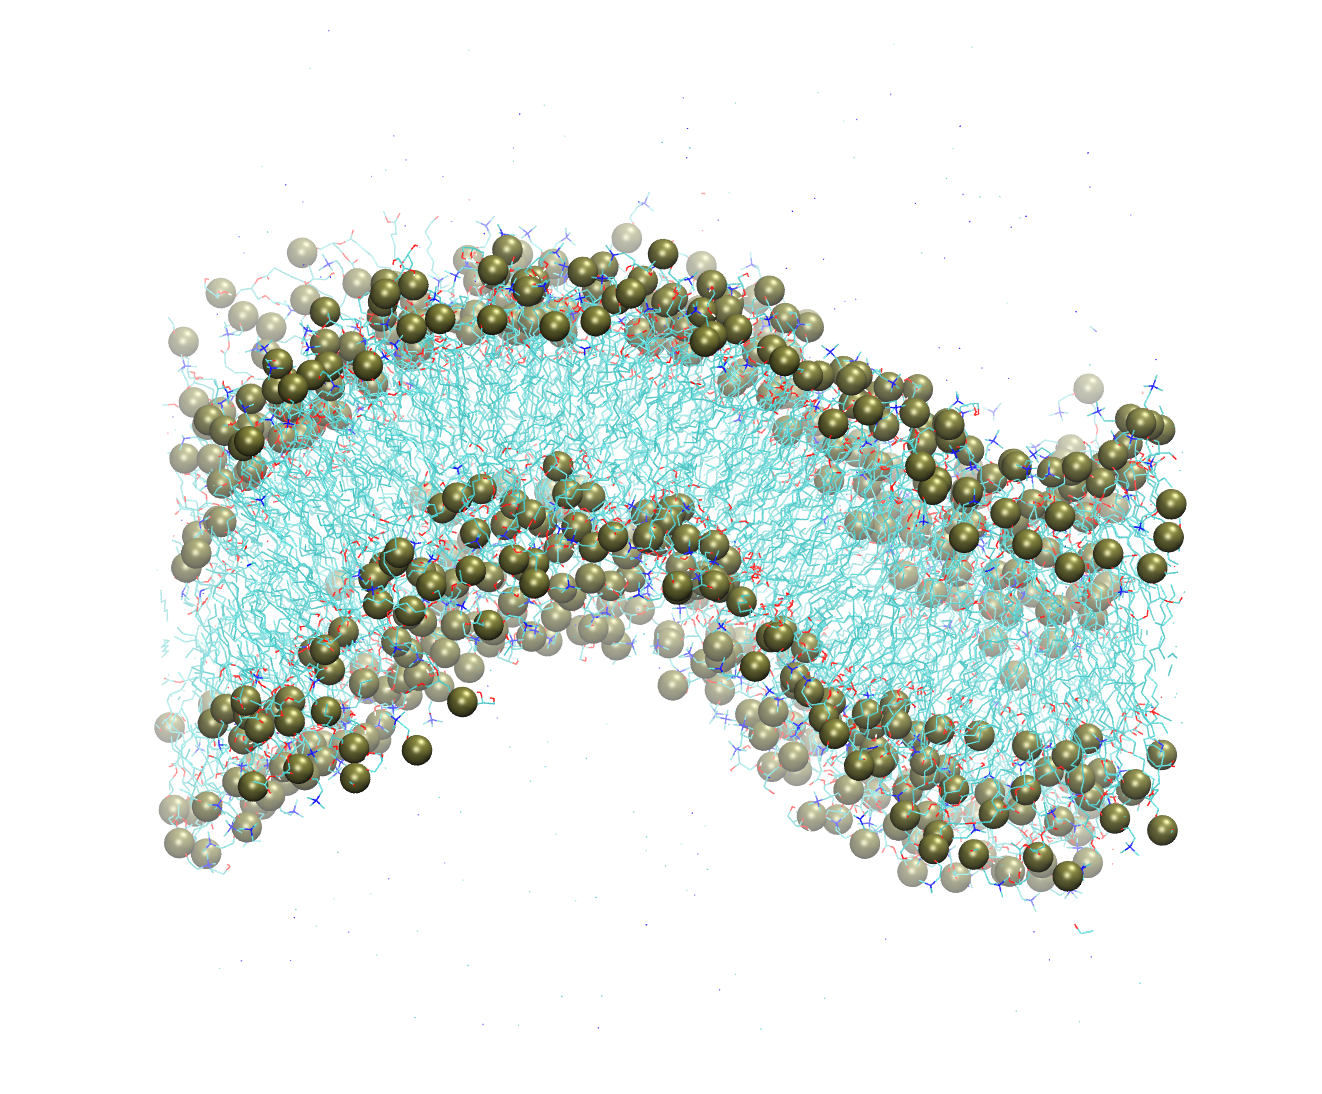
\includegraphics[width=44mm]{3results_capsule/pics/cg-130_600ns.png} \label{fig:pore_pics_1}}
\end{minipage}
\begin{minipage}[b]{0.4\linewidth}
\centering
\subbottom[]{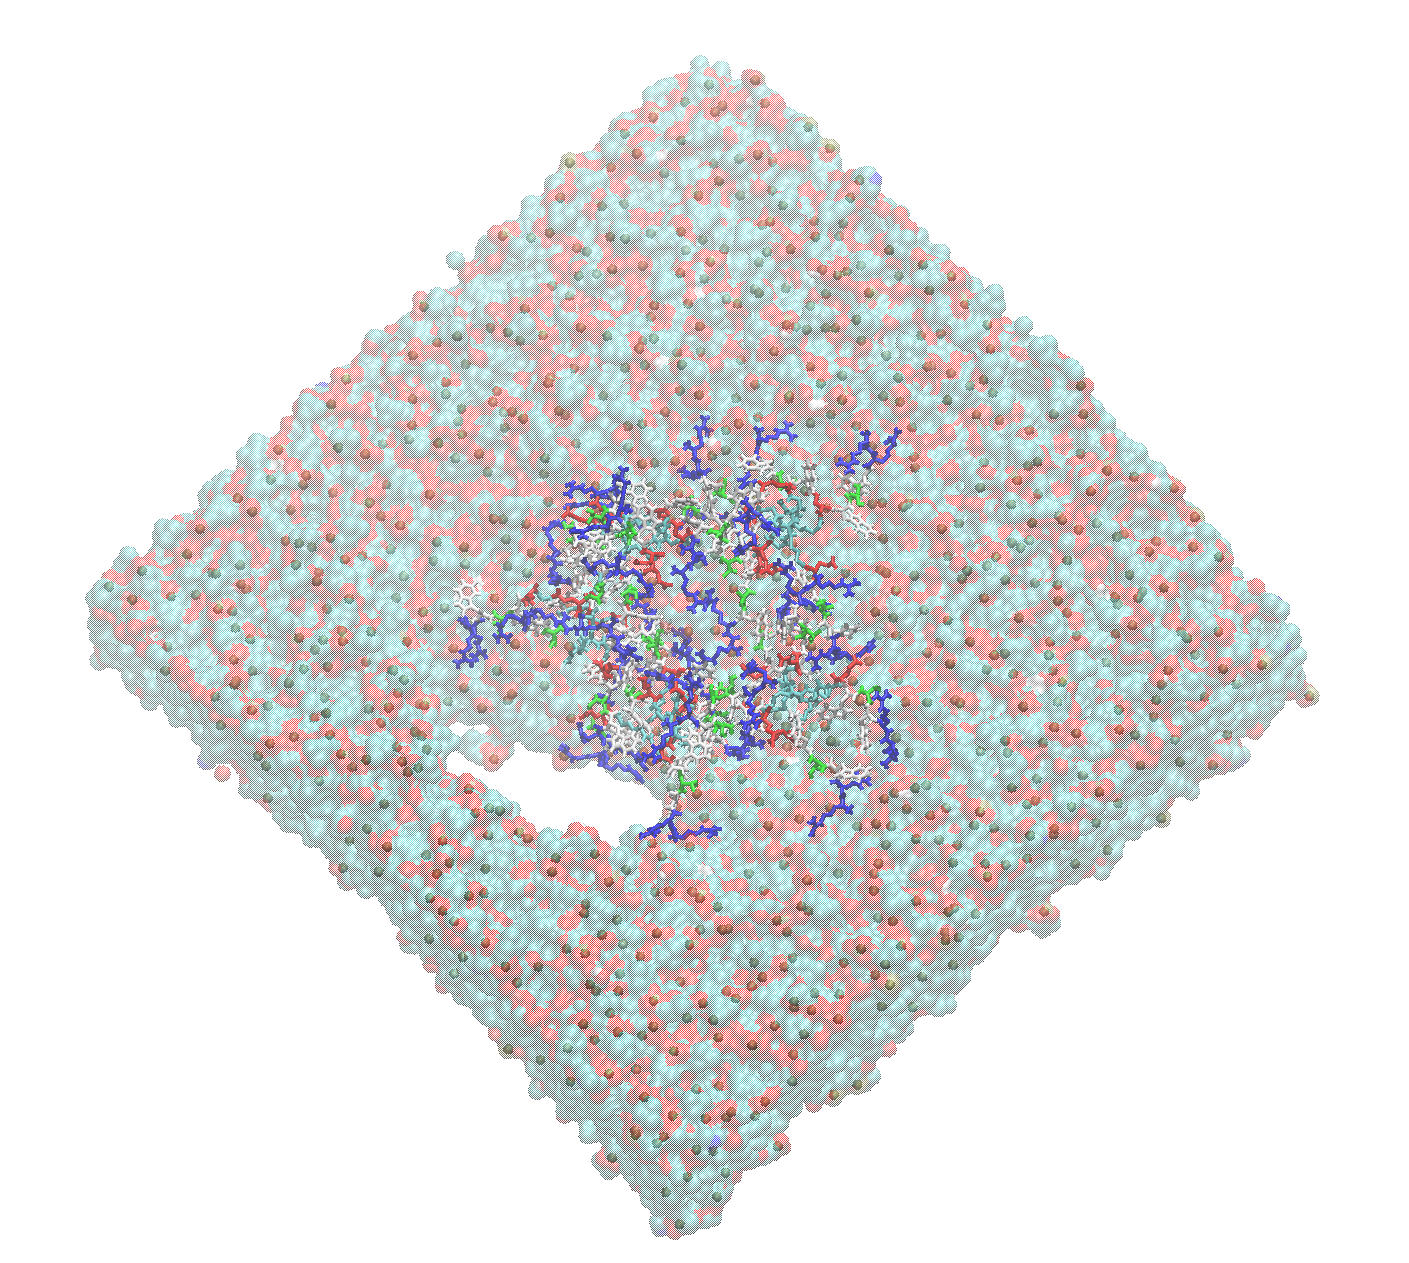
\includegraphics[width=59mm]{3results_capsule/pics/pore_large_130.png}
\label{fig:pore_pics_2}}
\end{minipage}
\begin{minipage}[b]{0.26\linewidth}
\centering
\subbottom[]{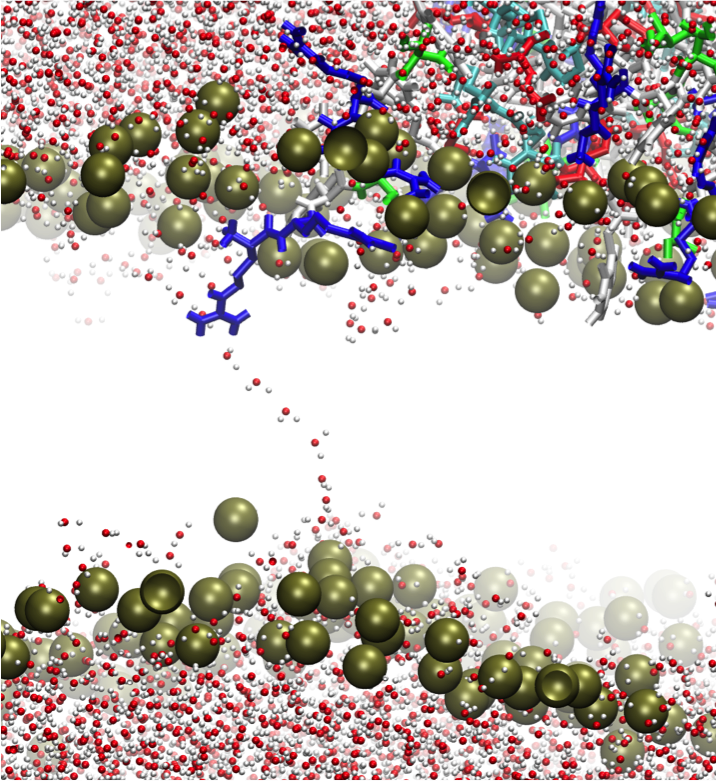
\includegraphics[width=39mm]{3results_capsule/pics/pore_arg.png}
\label{fig:pore_pics_3}}
\end{minipage}
\caption[Snapshot from relevant membrane-peptide atomistic simulations]{(a) Bacterial membrane deformation due to an electric field applied to the membrane (512 lipids, E = 130 mV/nm). (b) Pore formation due to the action of the peptide and electric field of 130 mV/nm. (c) Pore precursor due to Arginine insertion and water penetration. [VMD software, \citet{HUMP96}]}
\label{fig:pore_pics}
\end{figure}

As a control, a pure 512-lipid bacterial membrane was simulated under the same conditions, in three replicas: in the 600 ns runs, we observed the appearance of curved regions (Figure \ref{fig:pore_pics_1}) but no poration.
%
The appearance of a curvature made it necessary to compute the area per lipid taking this into account, as explained in Section \ref{sec:analysis}. The three replicas gave values of 0.520 nm$^2$, 0.514 nm$^2$ and 0.550 nm$^2$. Their discrepancy is due to the different level of curvature the membrane adopts during the runs (as they can change at a fast pace, the values given above were computed over the last 10 ns of the trajectory only).
%
It is observed that once a curvature appears it can be quickly enhanced by the electric field. Small casual variations in its initial onset can bring to very different shapes of the membrane and thus of compression of the lipids in it, giving different ApL values.

The electroporation threshold for the bacterial membrane alone was set at the higher value of 140 mV/nm: out of three simulations run with such value of the electric field, two resulted in disruption at 150 ns and 154 ns, while the third presented a curved but still intact membrane after 200 ns.
%
This shows that the effect of the field combined with the presence of the peptide accelerates the disruption process. Because of that, a slightly lower field value was sufficient to observe poration when the peptide was present.

The simulations with high electric field performed on the 512-lipid bilayer resulted all in curved geometries before the poration event (independently from the presence of the peptide). However this does not happen with the larger membrane, for which the poration was always initiated from a flat conformation (Figure \ref{fig:pore_pics_2}).
%
To rule out once more the hypothesis that the difference is due to the force field used (GROMOS 54A7 versus 54A8), we run an additional control simulation of the 512-lipid bilayer with the 54A8 force field and the electric field set at the electroporation threshold of 140 mV/nm. The bilayer, which was not electroporated in the 200 ns run, developed a curved shape similar to the outcome from the corresponding 54A7 simulations.
%
Also, the ApL values of the two simulations of the 512-lipid bilayer with peptide and a 140 mV/nm electric field, differing only for the force field (54A7 or 54A8), are quite similar: 0.554 versus 0.556 nm$^2$, computed taking into account the curvature.
%
However, from the previous discussion it emerges that there is a high variability in the ApL computed from highly curved configurations, so that the consistency of the two values might be fortuitous.
%
In any case, this analysis proves that the size of the bilayer has a large influence in the outcome of the simulations.

Regardless the shape that the membrane assumes before disruption, the peptide speeds up the membrane disruption. This is due to the charged Arginine residues which insert into the membrane core interacting with the negatively charged phosphate group of the lipids. They form hydrogen bonds with the ester groups, promoting the penetration of water molecule (Figure \ref{fig:pore_pics_3} and Supplementary Movies SI\_M4).
%
The precursor of this mechanism can be seen also in the simulations without or with low electric field (20 mV/nm): indeed, the vast majority of hydrogen bonds between Arginine and lipids listed in Table \ref{table:hb_pr_lip} involves the oxygen of the ester or phosphate group of the lipids, as shown in Table \ref{table:hb_ester}. This is also consistent with the deeper insertion observed for Arginine residues with respect to other ones (Figure \ref{fig:aa_insertion_bact}).

The positive charge of Arginine residues makes its behaviour within the membrane complex: Arginine residues buried in the membrane, can either bend their chain to re-surface in solution (in a process called snorkelling \citep{Liang2005,Ulmschneider2017arg,Ojemalm2016}), or make interaction with the phosphate and carbonyl groups, as observed in our simulations. The second option has been observed for Arginine rich antimicrobial or cell penetrating peptides through NMR experiments which measured the distance between the nitrogen of Arginine and the Phosphorus of lipids \citep{Tang2007,Jobin2019} and it was confirmed by MD simulations of the same or similar systems \citep{Herce2009,Jobin2019}, consistently with what found in this work.


\begin{figure}[t!]
\centering
 \def\arraystretch{1.6}
\begin{tabular}{lcccccccc}
\multicolumn{9}{c}{\textbf{Arg Capzip - DLPC/DLPG lipids hydrogen bonds}} \\
\hline
\multicolumn{2}{l}{\multirow{2}{*}{[$\tau \ge 50$\%]}} & \multicolumn{3}{c}{\textbf{E = 0 mV/nm}} && \multicolumn{3}{c}{\textbf{E = 20 mV/nm}} \\
\cline{3-9}
&& Total & Pho & CO$_n$ && All & Pho & CO$_n$ \\ 
\hline
DLPC && 20 & 6 & 14 && 18 & 10 & 8 \\
DLPG && 12 & 3 & 9 && 16 & 5 & 10 \\
\hline
 \end{tabular}
\captionof{table}[Hydrogen bonds between capzip Arg residues and DLPC/DLPG (atomistic)]{Number of the hydrogen bonds between Arginine residues and lipids, existing for more than 50\% of the time, in simulations of the 740-lipid bacterial bilayer with the peptide and electric field equal to zero or 20 mV/nm. Total number is displayed and the ones occurring with the Phosphate (Pho) moiety of the lipids or one of the ester groups (CO$_n$).}
\label{table:hb_ester}
\end{figure}

Finally, capzip causes a slight deformation on the shape of the membrane. This, together with the Arginine insertion, allows pore formation at a value of the electric field lower than the one necessary for electroporation.

Therefore, the presence of capzip has two main effects: it decreases the membrane fluidity (as measured by the reduction of the diffusion coefficient around the peptide), and makes the bilayer more sensitive to electric field, favouring the formation of water channels - two effects which are likely correlated, and which contribute to trigger its membrane disrupting activity.


\subsection{Atomistic simulations of the mammalian model membrane} \label{sec:lip_atom_mamm}

After the investigation of a model bacterial membrane, we focussed on a mammalian one, modelled as a DLPC membrane. We opted for a pure DLPC membrane to have a mammaloan model as close as possible to the bacterial one (DLPC/DLPG), to reduce the number of variables while testing the action of the peptide on these membranes. Thus, the mammalian counterpart was obtained selecting only the zwitterionic lipid species of the bacterial one. In turn, the bacterial model composition was selected to be the same as in the Supported Lipid Bilayers experiments \citep{Castelletto2016}.
%
Given the information accumulated in the previous investigation, we simulated directly a large bilayer (748 lipids), as we deemed this size more appropriate to run the subsequent simulations with the peptide. The force field employed is GROMOS 54A8 \citep{Reif2012}.

The properties of the stand alone membrane are computed as before and compared with the experimental data. Indeed for mono-lipid membranes several experimental results are available. The computed ApL is 0.592(3) nm$^2$, while the experimental range at 303 K of temperature is 0.608-0.632 nm$^2$ (see Table 1 in \citet{Poger2016}). To motivate the discrepancies, two factors must be considered. First, these experiments are performed on a variety of lipid geometries, from vesicle to Supported Lipid Bilayers (resting on a solid surface), justifying the broad range of values. Second, the membrane is simulated in presence of a 150 mM salt concentration, while the experiments do not adopt it. Several computational studies found a reduction of area per lipid when salt concentration is introduced \citep{Bockmann2003,Jarerattanachat2013,Reif2017}. This is consistent with the experimental evidence \citep{Pabst2007}, however, \citet{Reif2017} reported that simulations often overestimate this variation.

The fact that salt is responsible for the reduction in ApL is supported by the results from a simulation of a 512-lipid DLPC bilayer without salt, which gives ApL of 0.626(5) nm$^2$, compatible with the experimental values (see Table \ref{table:dlpc_apl} for a summary. To be noticed though that we are comparing two different sizes). Analogously, simulations of the 512-lipid bacterial model membrane without salt gave ApL of 0.596(5) nm$^2$, which is 3\% higher than the values found with a 150 mM concentration of NaCl (0.579(5) nm$^2$).
%
Moreover simulations performed without salt (see Chapter \ref{chapter:lip_par} show a better agreement with the experimental values.
%
Therefore, we conclude that the effect of the salt concentration is responsible for the smaller ApL observed for the large DLPC membrane simulated with 150 mM NaCl with respect to the experimental values. 

The ApL of the DLPC bilayer is larger than the one found for the model bacterial membrane, likely because the presence of DLPG in the latter diminishes the repulsion between the positively charged Choline heads of DLPC. Accordingly, the pure lateral diffusion (0.495(1) $\mu$m$^2$/s) is slightly higher than with what found for the mixed membrane (0.383(1) $\mu$m$^2$/s for DLPC and 0.487(3) $\mu$m$^2$/s for DLPC). Simulations of a 512-lipid DLPC bilayer without salt (see Figure 8 in Chapter \ref{chapter:lip_par}) gave a higher diffusion value with respect to the 150 mM NaCl simulation, and again we deemed the presence of the salt responsible for this.

\begin{figure}[t!]
\centering
 \def\arraystretch{1.6}
\begin{tabular}{llcll}
\multicolumn{5}{c}{\textbf{Properties of DLPC - atomistic}} \\
\hline
Pept. & Lip. & C (mM) & ApL (nm$^2$) & D ($\mu$m$^2$/s) \\
\hline
-- & 748 & 150 & 0.592(3) & 0.673(1) (global) \\
-- & 748 & 150 & 0.592(3) & 0.495(1) (pure) \\
-- & 512$\,^a$ & 0 & 0.626(5) & 0.541(1) (pure) \\
\cline{2-5}
-- & Exp.$^b$ & 0 & 0.608-0.632 & 3 \\
\hline
10 & 748 & 150 & 0.592(4) & see Table \ref{table:dlpc_D_space} \\
\hline
 \end{tabular}
\captionof{table}[DLPC atomistic simulations - general properties]{Area per lipid and diffusion coefficient (global or pure) from atomistic simulations of a DLPC bilayers. Pept.: number of peptides; Lip.: number of lipids. $^a$ Run with RF long range electrostatics and 1.4 nm cut off. $^b$ Experimental values: area per lipid from Table 1 of \citet{Poger2016}, diffusion coefficients from \citet{Lindblom2009}.}
\label{table:dlpc_apl}
\end{figure}

The presence of the peptide does not affect the ApL of the DLPC bilayer, as it was observed for the bacterial counterpart (on the same system size). Computing the diffusion centring the trajectory with respect to the peptide, we observe a larger diffusion coefficient with respect to the one computed for the membrane alone, likely because of the movement of one leaflet with respect to the other. Moreover, the lipids closer to the peptide are still slowed down in their movement as observed in the bacterial membrane (Table \ref{table:dlpc_D_space}).

Analysing the number of hydrogen bonds formed with the peptide, there are 590 bonds, of which 19 present more than 50\% of the time. Of them, 11 involve Arginine residues coordinated with ester or phosphate groups. These figures are smaller than the ones obtained for the bacterial membrane. In particular, the absence of the charged lipids makes the protein-membrane interaction less favourable. This is confirmed by the measure of the amino acid insertion (Figure \ref{fig:aa_insertion_mamm}) which are on average less inserted than into the bacterial membrane.

\begin{figure}[t!]
\centering
 \def\arraystretch{1.6}
\begin{tabular}{lllll}
 \multicolumn{5}{c}{\textbf{Diffusion for DLPC with capzip}} \\
 \hline
Pept. & Lip. & Region & Nr. & D ($\mu m^2/s$) \\
 \hline
10 & 748 & $d<1$ & 100 & 0.495(3) \\
10 & 748 & $d<2$ & 180 & 0.584(3) \\
10 & 748 & $d<3$ & 323 & 0.603(5) \\
10 & 748 & $d>3$ & 412 & 0.993(5) \\
10 & 748 & All & 735 & 0.821(2) \\
 \hline
 748 & 0 & All (B$_{COM}$) & 748 & 0.673(1) \\
 748 & 0 & All (L$_{COM}$) & 748 & 0.495(1) \\
 \hline
 \end{tabular}
\captionof{table}[Diffusion in proximity of capzip for DLPC bilayer (atomistic)]{Diffusion coefficients of lipids, in a mammalian model membrane. Pept.: number of peptides; Lip.: number of lipids; Region: the values are computed for groups of lipids which, at the initial time, were within 1 nm, 2 nm, 3 nm from the peptide or further away. D is computed centring the trajectory around the Protein COM, when this is present. The pure and global coefficients are given for the pure membrane. Error from linear fit in parenthesis.}
\label{table:dlpc_D_space}
\end{figure}

The investigation performed on the bacterial model membrane sets to 130 mV/nm the threshold electric field needed to observe poration at the atomistic level on such membrane (with the GROMOS force field). Therefore, we want to reproduce this condition on a DLPC model membrane and see whether the influence of capzip is smaller on the DLPC membrane with respect to the DLPC/DLPG.
%
However, for the DLPC membrane this value was sufficient to cause poration both with and without peptide. Despite the absence of lipids with a net charge, which are expected to interact more strongly with the electric field, this membrane seems more sensitive to such external perturbation. We think this is due to larger ApL: indeed, being the lipids less packed, water penetration is easier. This, combined with the electric field, generates more easily water channels which promote pore formation.

In the case of the mammalian model membrane, we observed that, once the membrane starts disrupting, the peptide detaches from it, while it remained firmly attached in the simulations with the bacterial one, following its deformations. This lower propensity for binding on the mammalian case will be proven also by coarse-grained simulations and is consistent with the previous analysis on hydrogen bonds propensity and amino acids insertion. Moreover it confirms that the poration is induced because of the high electric field rather than the presence of the peptide. We do not pursue the investigation of the electroporation threshold for the DLPC membrane, as we focussed here only on the action of the peptide on it.
%
Finally, in interpreting these results, it must be considered that the transmembrane potential of a mammal cell is lower than the one present in the bacterial membrane \citep{Yeaman2003,Wilson2011}, so that their membranes usually need to withstand milder electric field conditions than bacterial ones.


\subsection{CG simulations of the buckyball on model membranes} \label{sec:results_lip_cg}

\paragraph{Standard MARTINI simulations} Coarse-grained simulations allow to model the behaviour of the full capsule interacting with the membrane.
%
At first, simulations with the standard MARTINI model were run, as they have higher computational speed with respect to the Polar MARTINI model. To be noticed that the full system, comprising a 2880 lipids bilayer and the capsule, measures approximately 30 nm along each side of the simulation box.

The coarse-grained simulations of the full buckyball bilayer on a DLPC/DLPG membrane (3:1 ratio) confirms the binding of the peptide on the latter, driven by charge-charge recognition: in both the replicas run, the peptide approaches the membrane after about 2 $\mu$s, remaining bound for the remaining of the 10 $\mu$s simulated.
%
Post-binding, the capsule diffuses on the membrane and produces an increasingly high curvature on it, in a process which tends to maximize the contact area (see Figure \ref{fig:pL6_vmd_2} and Supplementary Movies SI\_M5). No poration is observed, probably due to the force field characteristics which stabilise the structure of both the membrane and the peptide assembly. Additionally, longer time scales might be needed to observe it. Later in this section, we will analyse simulations performed with an externally applied electric field, in line with what done in the atomistic case, which speeds up the process and allow to observe membrane disruption.

\begin{figure}
\centering
\vspace{1.5cm}
\scriptsize
 \def\arraystretch{1.6}
\begin{tabular}{lllllllll}
& \multicolumn{8}{c}{\textbf{Properties of DLPC/DLPG - MARTINI}} \\
 \hline
& Pept. & Lip. & C & E & FF & ApL & D$_{DLPC}$ & D$_{DLPG}$ \\
& & & (mM) & (mV/nm) & & (nm$^2$) & ($\mu$m$^2$/s) & ($\mu$m$^2$/s) \\
% Pept. & Lip. & C (mM) & E (mV/nm) & FF & ApL (nm$^2$) & D$_{DLPC}$ ($\mu$m$^2$/s) & D$_{DLPG}$ ($\mu$m$^2$/s) \\
 \hline
\textbf{1} & -- & 2880 & 0 & -- & MA & 0.581(3) & 75.84(7) & 76.64(5) \\ 
\textbf{2} & -- & 2880 & 150 & -- & MA\_P & 0.611(1) & 79.4(4) & 79.0(5) \\
\textbf{3} & -- & 2880 & 150 & 20 & MA\_P & 0.614(1) & 74.64(5) & 73.67(2) \\
\textbf{4} & -- & 2880 & 150 & 40 & MA\_P & 0.619(2) & 70.31(4) & 70.45(6) \\
 \hline
\textbf{5} & 120 (BB)$^b$ & 2880 & 0 & -- & MA & 0.582(1) & 74.28(1) & 73.34(2) \\
\textbf{6} & 120 (BB)$^a$ & 2880 & 0 & -- & MA & 0.581(2) & 70.51(1) & 62.59(2) \\ 
\textbf{7} & 120 (BB)$^a$ & 2880 & 150 & -- & MA\_P & 0.621(2) & 65.82(6) & 68.94(9) \\
\textbf{8} & 120 (BB)$^a$ & 2880 & 150 & 20 & MA\_P & 0.616(2) & 70.29(7) & 61.54(10) \\
\textbf{9} & 120 (BB)$^a$ & 2880 & 150 & 40 & MA\_P & \multicolumn{3}{c}{Poration} \\
\hline
&\multicolumn{8}{c}{} \\
&\multicolumn{8}{c}{\textbf{Properties of DLPC - MARTINI}} \\
 \hline
& Pept. & Lip. & C & E & FF & ApL & D$_{DLPC}$ & \\
& & & (mM) & (mV/nm) & & (nm$^2$) & ($\mu$m$^2$/s) & \\
 \hline
\textbf{1} & -- & 2888 & 0 & -- & MA & 0.590(2) & 83.5(3) \\ 
\textbf{2} & -- & 2888 & 150 & -- & MA\_P & 0.608(2) & 80.5(4) & \\
\textbf{3} & -- & 2888 & 150 & 20 & MA\_P & 0.610(1) & 78.3(1) & \\
\textbf{4} & -- & 2888 & 150 & 40 & MA\_P & 0.614(1) & 76.90(3) & \\
 \hline
\textbf{5} & 120 (BB) & 2888 & 0 & -- & MA & 0.590(1) & 81.07(3) & \\ 
\textbf{6} & 120 (BB) & 2888 & 150 & -- & MA\_P & 0.608(1) & 70.52(2) &  \\
\textbf{7} & 120 (BB) & 2888 & 150 & 20 & MA\_P & 0.611(1) & 75.28(6) & \\
\textbf{8} & 120 (BB) & 2888 & 150 & 40 & MA\_P & 0.616(1) & 77.88(4) & \\
 \hline
\end{tabular}
\vspace {0.5cm}
\captionof{table}[Properties of DLPC/DLPG and DLPC membranes (MARTINI)]{Properties of DLPC/DLPG (top) and DLPC membrane (bottom) in MARTINI simulations with and without capzip. Pept.: number of peptides (BB - buckyball bilayer). Lip.: number of lipids; FF: force field (MA - MARTINI; MA\_P - Polar MARTINI).
%
D is computed removing the centre of mass movement of the bilayer for simulations without the capsule, and movement of the protein for simulations where the peptide is bound to the membrane. For DLPC/DLPG, the buckyball bilayer binds to the membrane: values marked with $^b$ are computed \emph{before its binding}, with $^a$ \emph{after the binding}.
%
For DLPC it never binds and the values are computed \emph{for the whole simulation length} (discarding the first 100 ns).}
\label{table:martini_diff}
\vspace{1.5cm}
\end{figure}

The area per lipid was computed taking into account the curvature (as explained in Section \ref{sec:analysis} and in \citet{Braun2011}), and does not change significantly in presence of the capsule.
%
When analysing the diffusion coefficient, the values obtained for pure membranes (or before the binding) have been computed removing the bilayer centre of mass movement, while the ones with the capsule bound to the membrane by centring the trajectory around it (and considering the portion of the trajectory after the binding only). The MARTINI diffusion coefficients are about 60 times larger than the ones obtained atomistically (Table \ref{table:martini_diff}), due to the coarse-grained parametrisation. The values are consistent with results obtained on a variety of other systems tested by \citet{Venable2017} in a study of diffusion for MARTINI simulations.

The diffusion coefficients obtained for simulations of the pure membrane and for simulations with the buckyball bilayer before its binding (lines 1 and 5 in Table \ref{table:martini_diff}, top) are similar for the DLPC/DLPG membrane and shows that the two lipids diffuse at the same pace.
%
The lipids diffusion is instead decreased after binding of the buckyball bilayer, by 5\% for DLPC and by 15\% for DLPG (line 6 of Table \ref{table:martini_diff}, top). The larger effect on DLPG is due to the attraction between the peptide and this negatively charged lipid: computing the RDF of the phosphate beads (PO4) of DLPC and DLPG around the protein, a much stronger signal comes from DLPG beads rather than DLPC ones (Figure \ref{fig:PO4_RDF}), showing they are more attracted toward the peptide.

The mechanism above results in the slower diffusion of the DLPG residues nearby the capsule, as already predicted at the atomistic level. Moreover, the coarse-grained simulations allow to see the recruitment of negatively charged lipids nearby the capsule: Figure \ref{fig:PO4_dens} shows a lateral density profile of the two lipid species across the simulation box. Spanning the $x$ axis, the DLPG density increases around the position of the capsule, at the expenses of the DLPC one. The formation of a DLPG patch enhances the slowing effect on the diffusion of this species, while DLPC, pushed away from the capsule location, is less perturbed.

\begin{figure}[t!]
\centering
\subbottom[]{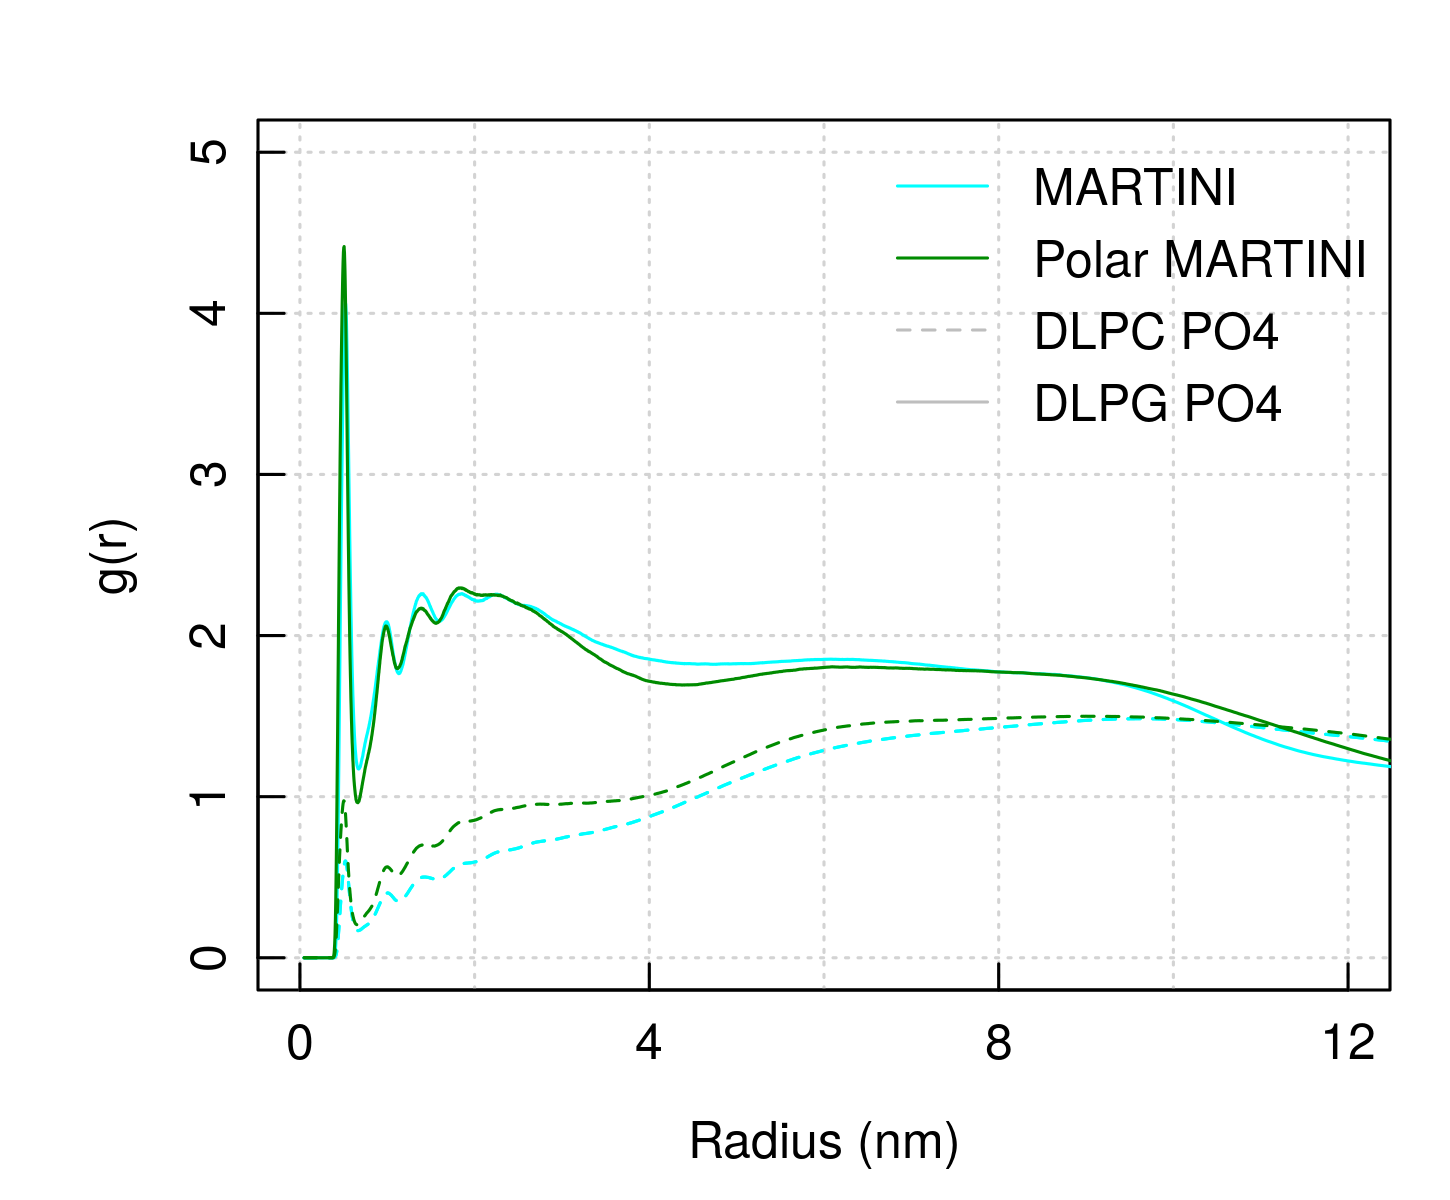
\includegraphics[width=0.45\linewidth]{3results_capsule/pics/RDF_PO4_around_Prot.png} \label{fig:PO4_RDF}}
\subbottom[]{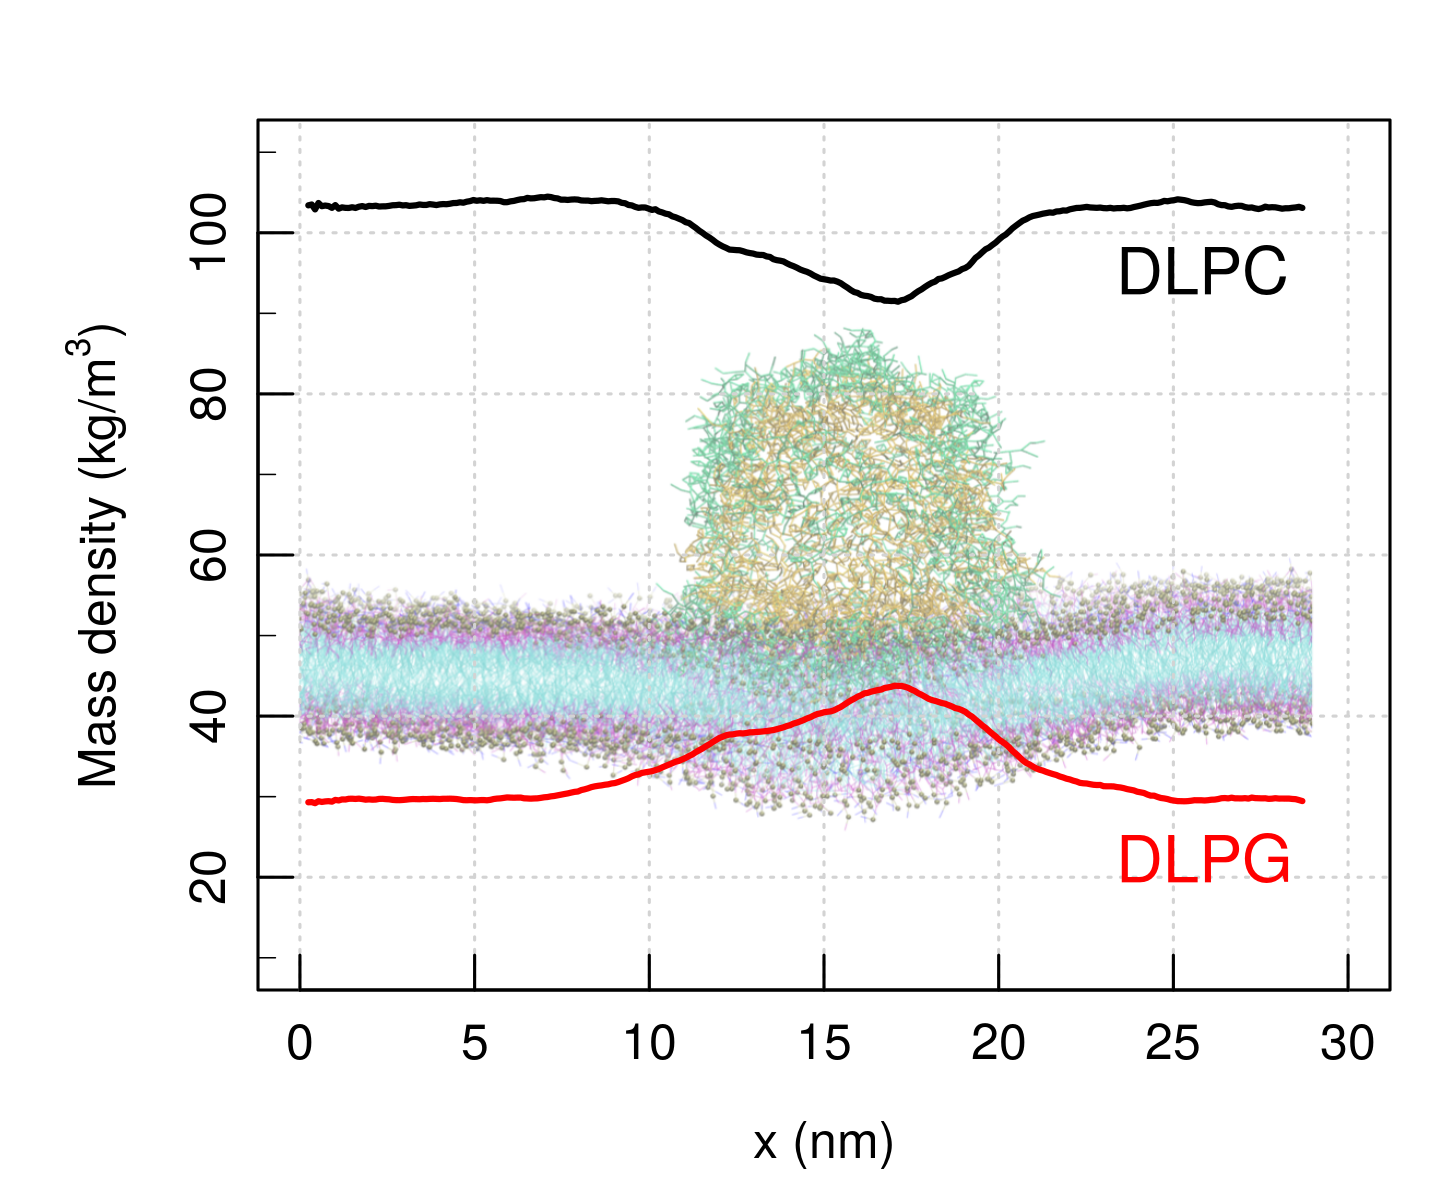
\includegraphics[width=0.45\linewidth]{3results_capsule/pics/densX2.png} \label{fig:PO4_dens}}
\caption[Proximity of lipids phosphate to bound capsule (MARTINI simulations)]{(a) RDF of phosphate bead (named PO4 in both MARTINI models) of DLPC and DLPG around the Protein. (b) Mass density of DLPC and DLPC in a DLPC/DLPG membrane along the $x$-axis, computed for simulations of the membrane with the buckyball bound to it. Superimposed is a picture of the corresponding configuration.}
\label{fig:PO4_RDF_dens}
\end{figure}

To conclude the investigation performed with standard MARTINI, we simulated the capsule together with a pure DLPC membrane. The capsule does not bind to the latter in the 10 $\mu$s simulated (Supplementary Movies SI\_M6): it comes close to it multiple times, keeping an average distance of 3 nm and a minimum of 1 nm (Supplementary Figure \ref{fig:mindist_buck_dlpc}). This, together with what already observed in the atomistic simulations, suggests once more that the interaction with non charged lipids is not leading to attachment of the buckyball to the membrane.

\paragraph{Polar MARTINI simulations} 
Polar MARTINI simulations focussed on \emph{in silico} experiments with an external electric field, to set a parallel with the analogous investigation performed at the atomistic level. The addition of an external electric field is not possible in standard MARTINI simulations because standard water does not provide a long range electrostatic screening. As such, the electric field effect would be overestimated.
%
Together with the simulations of the membrane with the capsule, we run control simulations of the pure membrane with the selected values of the external field, to exclude the possibility of electroporation.

Simulations on the membranes alone (both the bacterial and mammalian model) showed an increased ApL with respect to the standard MARTINI simulations (lines 1-2 in Tables \ref{table:martini_diff}, top and bottom). This is the opposite of what observed in the test case run in the original work that parametrised Polar water \citep{Yesylevskyy2010}, possibly due to the different size and composition of the test membrane used.
%
Additionally, the two simulations are run with different values of the salt concentration (MARTINI has only counter ions, Polar MARTINI has 150 mM NaCl): in the atomistic case this discrepancy made the ApL decrease, which is again inconsistent with what observed here and can be attributed to the parametrisation of ions in the coarse-grained model (e.g.\ their van der Waals radius includes the first hydration shell, thus they will penetrate less easily into the lipid head region).
%
Regarding the diffusion coefficient it decreases from MARTINI to Polar MARTINI, despite an increase in ApL, and this is likely due to stronger interactions between lipids (especially the charged DLPG). This is due to the Coulomb interaction, which is less screened and thus stronger in the Polar MARTINI model.

When an electric field is applied in Polar MARTINI simulations, there is a slight increase of ApL for higher values of it, but the diffusion decreases slightly (lines 2-4 in Tables \ref{table:martini_diff}, top and bottom). In atomistic simulations the field decreased the ApL for small systems and had negligible effect for larger ones; while the diffusion was reduced, as in the Polar MARTINI case.

To simulate the binding of the buckyball bilayer, we first focussed on the bacterial membrane. We run one simulation without electric field, to test the interaction between the two with the new parametrisation. The binding happens much faster than what observed in the standard MARTINI simulations (within the first 50 ns), and the membrane starts to be deformed by the capsule already after 100 ns (Figure \ref{fig:martini_stMem0}). For this reason, Table \ref{table:martini_diff} does not report a value of the diffusion \emph{before} binding.

\begin{figure}[t!]
\centering
\subbottom[]{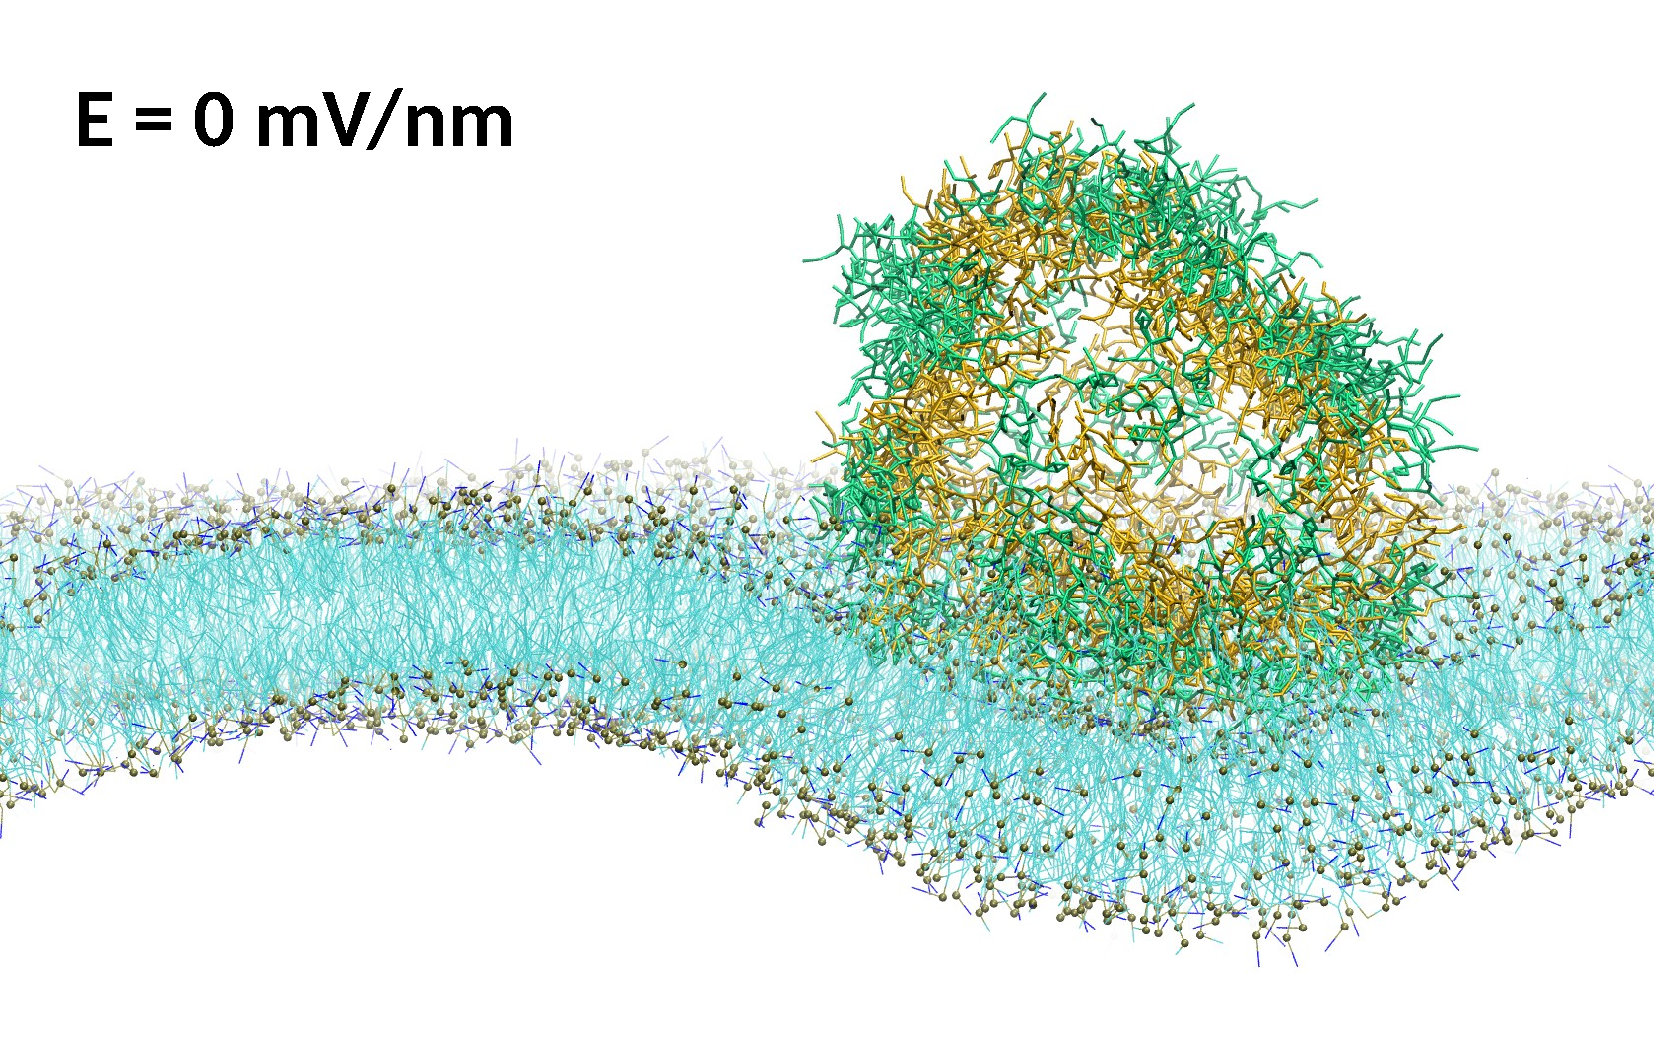
\includegraphics[width=0.45\linewidth]{3results_capsule/pics/stMemPWE0} \label{fig:martini_stMem0}}
\subbottom[]{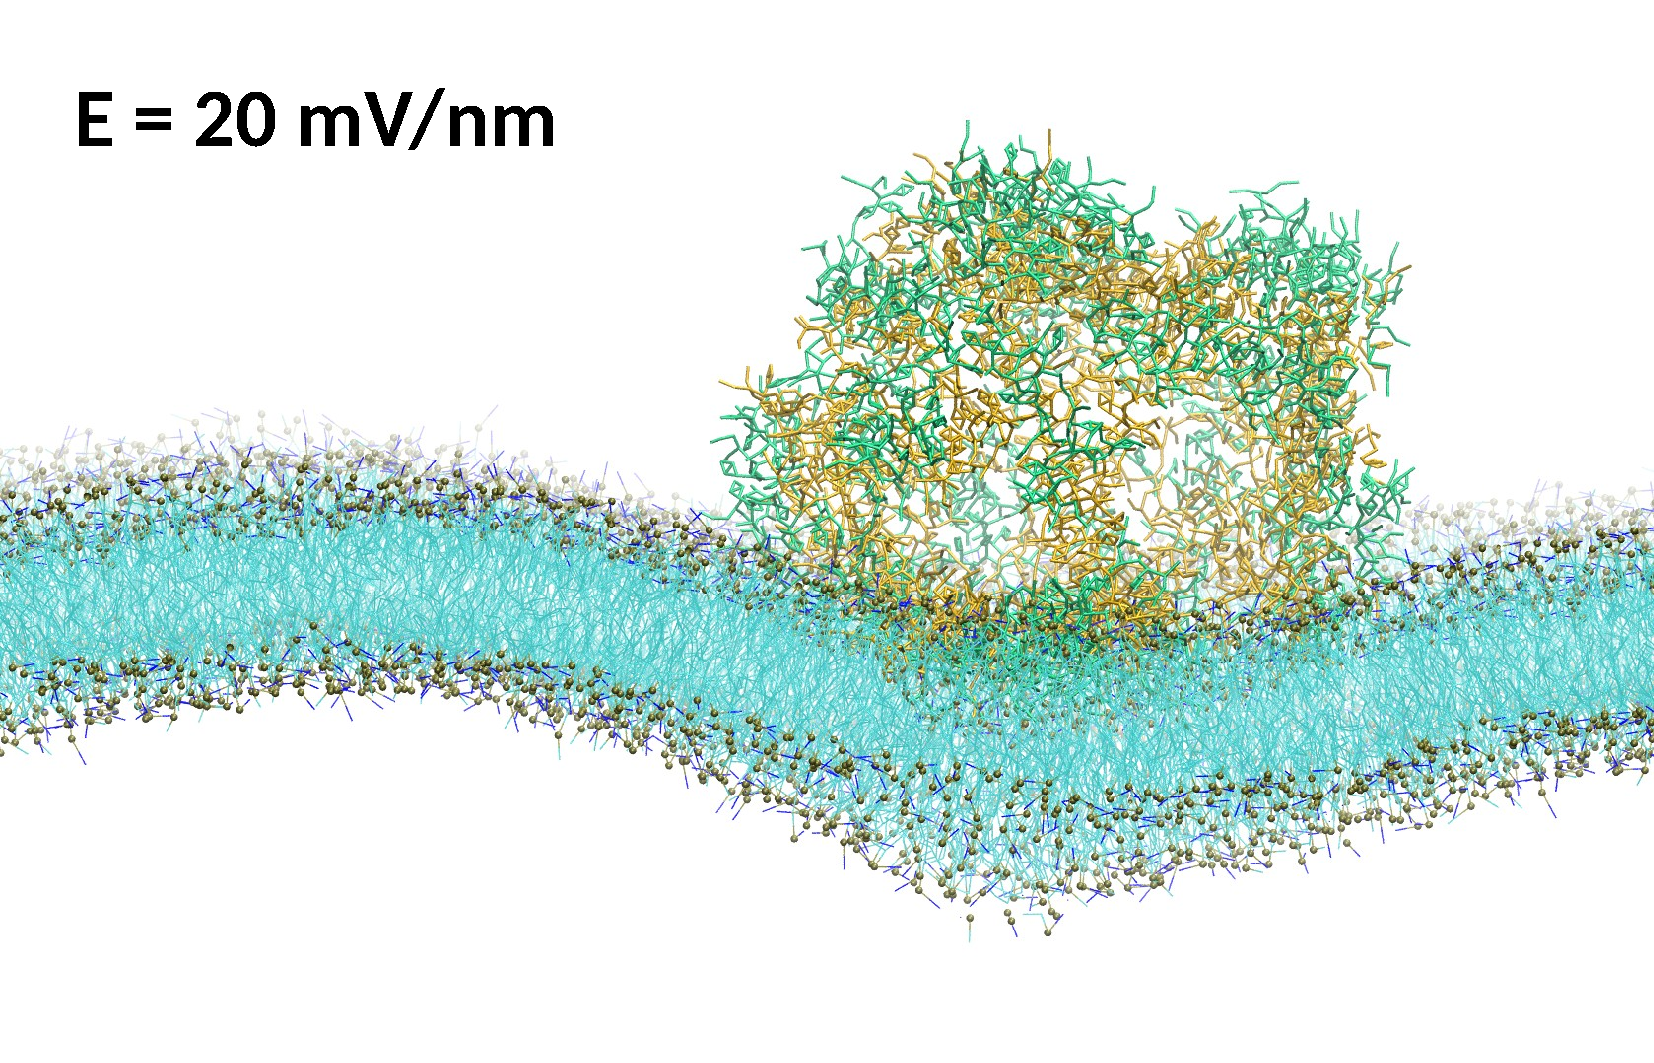
\includegraphics[width=0.45\linewidth]{3results_capsule/pics/stMemPWE20}  \label{fig:martini_stMem20}}
\caption[Bacterial membrane and buckyball bilayer (MARTINI simulations)]{Final configuration (500 ns) of Polar MARTINI simulations of a buckyball bilayer approaching and binding to a model bacterial membrane, spontaneously (a) or under the effect of a 20 mV/nm electric field (b). Capsule in bond representation, green external layer, yellow internal one. Lipids in line representation, phosphate beads in gold van der Waals. [VMD software \citet{HUMP96}]}
\label{fig:martini_stMem}
\end{figure}

We did not observe poration on the time scale of the simulation (500 ns): a longer simulation might allow to observe membrane disruption but, as mentioned before, we preferred to focus on the action of the electric field. As such, we simulated the binding under the action of a 20 mV/nm electric field. The curvature of the membrane is slightly more pronounced than in the case without field, but again no disruption happens in the 500 ns simulated (Figure \ref{fig:martini_stMem20}).
From the final configuration of this run we doubled the electric field, which was sufficient to observe poration within 200 ns.
%
Remarkably, a value of 40 mV/nm is within the physiological range of the transmembrane potential (which is around 35 mV/nm for the bacterial inner membrane, and 20 mV/nm across a mammalian membrane. See discussion in Section \ref{sec:details}).

As in membrane simulations the pressure coupling is performed semi isotropically, once a pore is formed, the box undergoes a large and unphysical deformation if the pore keeps expanding. The analysis of the events happening after poration are thus affected by this artefact.
%
To obviate to that, we took a frame at the early stages of pore formation (1 ns after the first formation of a water channel) and continued the run, with the same electric field, with isotropic pressure coupling. This allowed to observe the capsule penetrating the membrane in the first 10 ns from the beginning of this run (Figure \ref{fig:martini_poration} and Supplementary Movies SI\_M7): the lipids do not seal around the capsule, allowing the passage of water and ions, which is consistent with what found in the atomistic simulations. Moreover, in the passage, the capsule deforms and partially opens.
%
After this, the membrane is completely disrupted and the lipids rearranged into fibers ad micelles to shield their tails from the solvent, while some of them remain attached to the capsule (Supplementary Movie SI\_M7).

The fact that we observed poration at a much lower value of the electric field than what found with the atomistic model can be explained by several characteristic of the coarse-grained parametrisation: first, it favours a more dynamical rearrangement between lipids (see the discussion on diffusion in the following); second, it is known for smoothing the energy barriers and thus speeding up the course of events: the effective time sampled in MARTINI simulations is 3 to 6 times larger than the one actually simulated \citep{SiewertJ.Marrink2003}. Moreover, in these simulations the full capsule with 120 molecules is present, interacting with the electric field more strongly than the pentagonal subunit used in the atomistic simulations, which hosted 10 molecules only.

\begin{figure}[t!]
\centering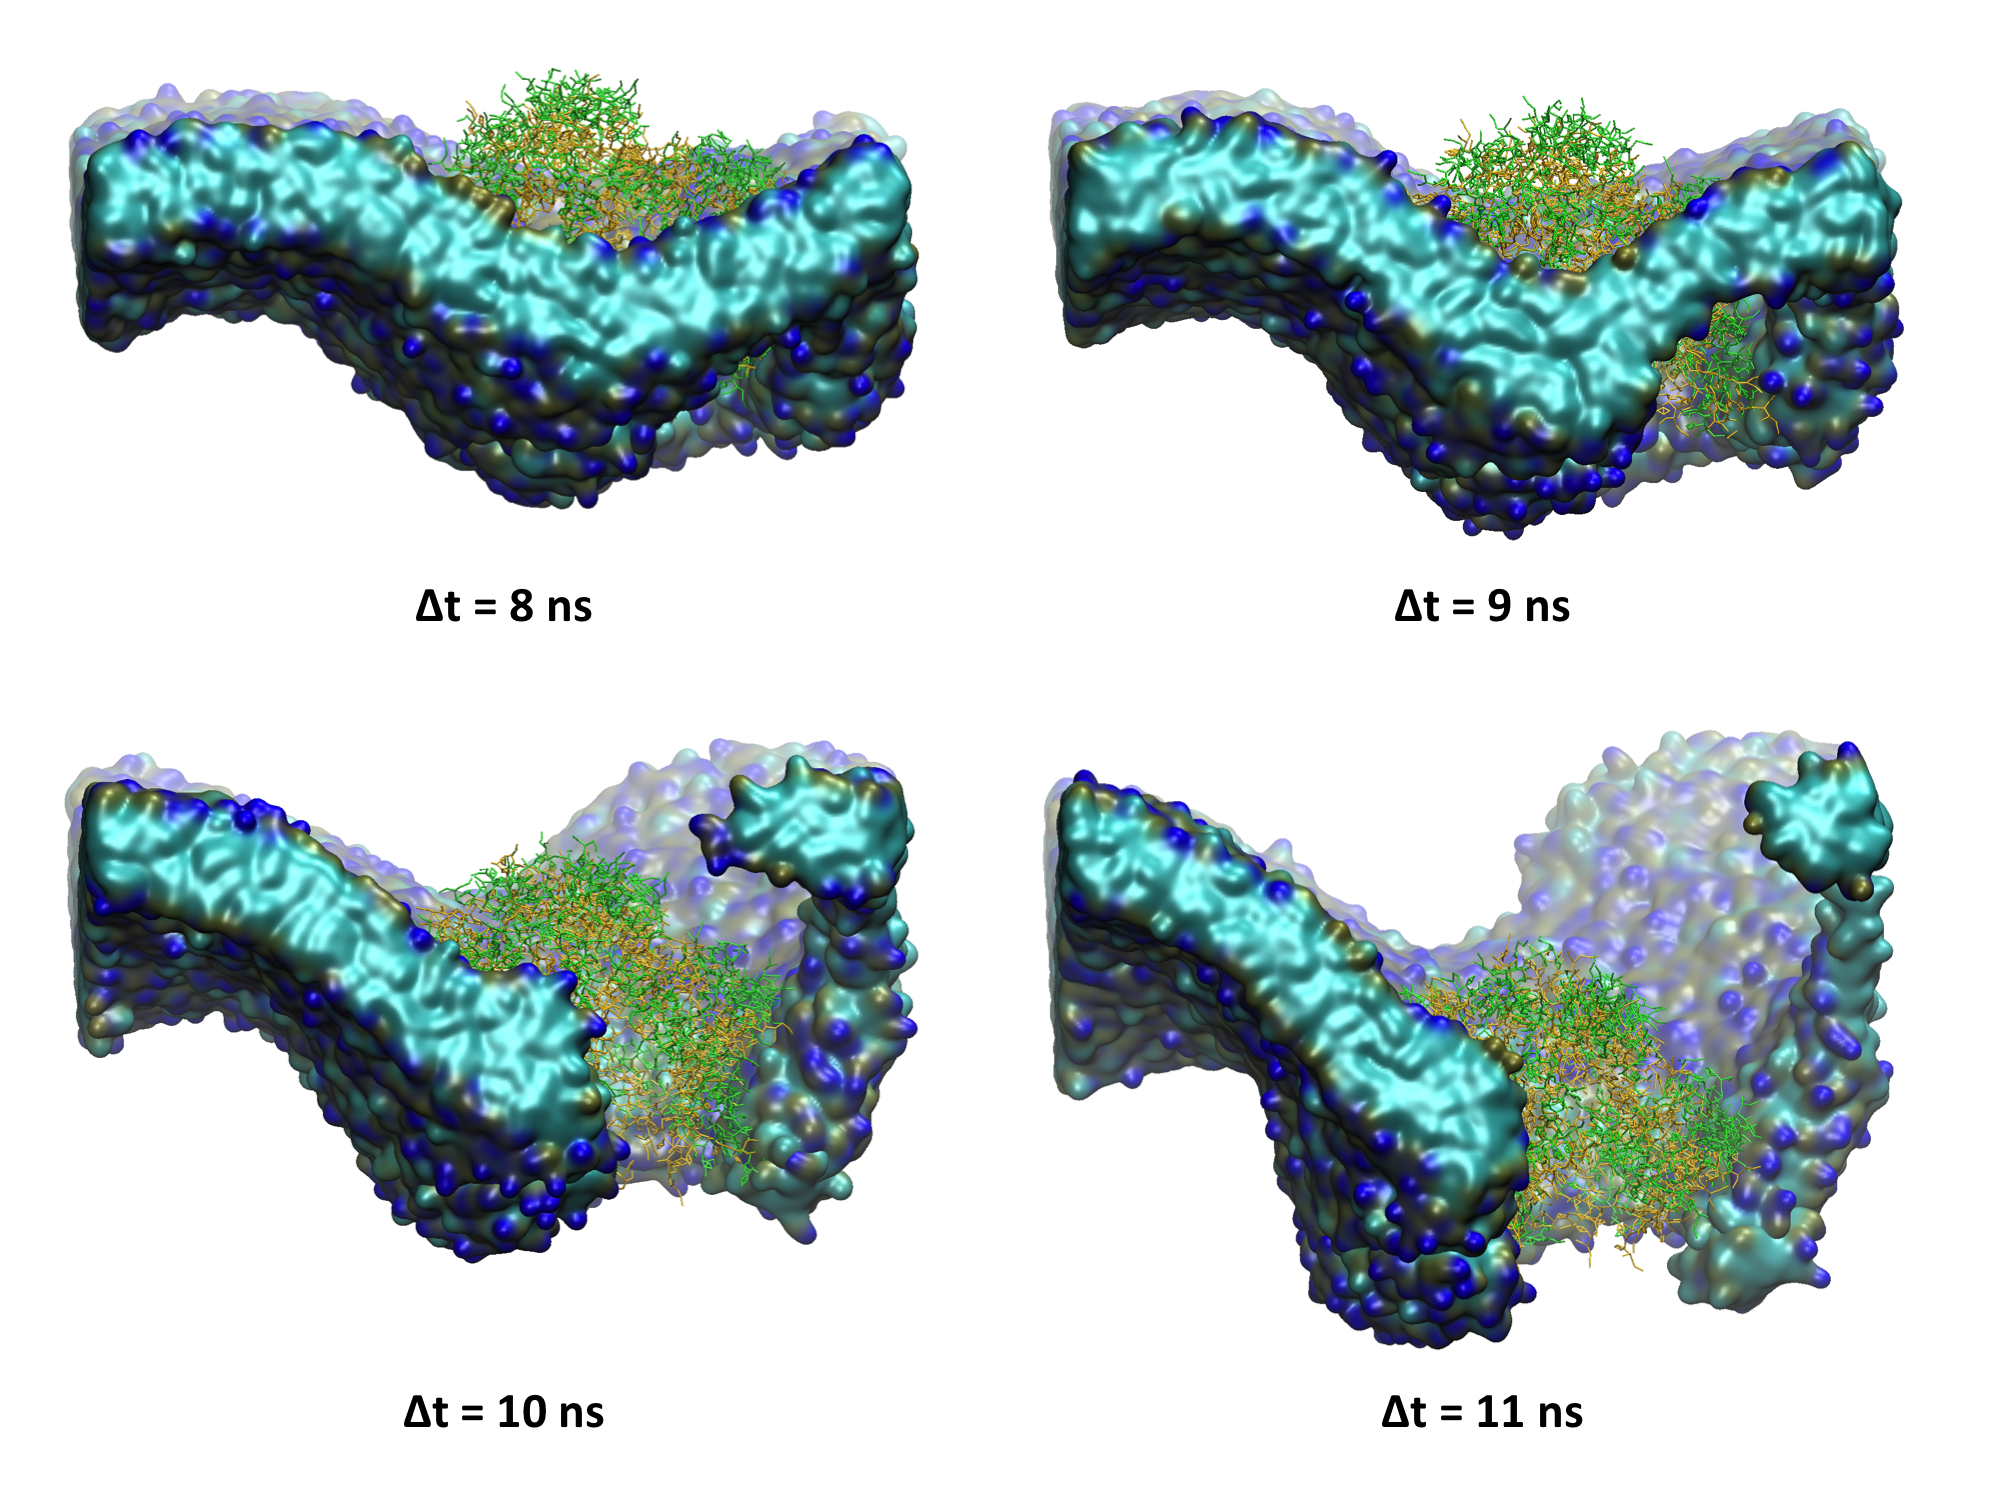
\includegraphics[width=0.95\linewidth]{3results_capsule/pics/poration_martini.png} 
\caption[Bacterial membrane poration (MARTINI simulations)]{Bacterial membrane poration due to the action of the capzip buckyball bilayer and an external electric field of 40 mV/nm (Polar MARTINI simulations). $\Delta t$ indicates the time from the beginning of the simulation performed with isotropic pressure coupling (started 1 ns after the formation of a water channel spanning the membrane). Capsule in bond representation, green external layer, yellow internal one. Lipids in surface representation. [VMD software \citet{HUMP96}]}
\label{fig:martini_poration}
\end{figure}

As a control, the same simulations with external electric field were run with a DLPC membrane: for none of the values tested (0, 20 and 40 mV/nm) the capsule attached to the membrane, as already saw in standard MARTINI simulations.
%
%This definitely prove that the peptide has a low propensity to bound to non anionic lipids. This can raise questions in the light of its tranfection properties, as it was experimentally demonstrated that capzip can enhance the internalisation of siRNA on HeLa cells. However, the siRNA material has a high negative charge, which can impact substantially the electrostatic profile of a capsule including it and thus on its binding more to membranes.

Regarding diffusion, we retrieved the slowing down of lipids when the buckyball bilayer is bound to the bacterial model membrane. DLPG is more slowed down with respect to DLPC in simulations with no or 40 mV/nm electric field, while for the 20 mV/nm it is slightly faster.
%
Instead, when considering the DLPC membrane simulated in presence of a capsule (which does \emph{not} bind to it), diffusion of lipids is increased with the field. This is the opposite to what observed for simulations of the DLPC membrane alone, showing that the buckyball bilayer has a long range interaction with the membrane and modifies its dynamics, even without binding to it. 

As a final comment, it must be noticed that the variability on the diffusion coefficient might be higher than what suggested from the error derived from the fit. The MSD computed on MARTINI membranes has a very precise linear dependence from time, thanks to the length of the simulation and the extent of the system (the MSD is averaged over many time frames and many lipids, see Figure \ref{fig:MSD_martini}). This gives a small error on the fitted slope. However for the MARTINI simulation of the capsule on DLPC/DLPG, we run a second replica and observed a discrepancy of about 2 $\mu$m$^2$/s between the diffusion coefficients, despite both have a very small error from the fit.
%
As such, the results presented in Table \ref{table:martini_diff} must be interpreted carefully. However, the differences between the DLPC and DLPG coefficients observed for the simulations after binding of the buckyball bilayer to the membrane are large enough to remain significant, confirming that the peptide has a stronger effect on negatively charged lipids.


\section{Outlook}
The investigation performed proved the power of the multiscale simulations approach to elucidate details of nanoscale systems which are otherwise inaccessible to experiments.

When investigating the assembly process of capzip molecules, the use of atomistic simulations gave insight into the role of each amino acid of the sequence in the pairing of many copies of the molecule. Coarse-grained simulations proved the stability of the hypothetical structure on the long time scale. Overall, we were able to conclude that the ability of capzip to form capsule lays not only in the scheme of opposite charges that it hosts along its arms, but also in the presence of many hydrophobic residues, which favour the assembly by hydrophobic effect.
%
Thus, the proposed structure contains a bilayer arrangement of the molecules, which is demonstrated to be more stable than a monolayer one, and is consistent with recent experimental findings showing multilayer capsules \citep{Kepiro2019}.

Coarse-grain simulations were also able to clarify the interaction of capzip with the membrane. Capzip has a propensity to bind to negatively charged membranes, which are a simplified model for the bacterial inner membrane, but not to zwitterionic lipids, which model a mammalian membrane. Moreover, on the bacterial membrane, the buckyball recruits the negatively charged lipids in its proximity, reducing their diffusion.

Atomistic simulations complemented these findings showing the details of such interaction: on a bacterial membrane, capzip interacts with the lipids forming many hydrogen bonds and inserting the Arginine side chains deep in the phosphate region of the lipids. Consequently, the lipids around the peptide are slowed down in their diffusion also on the time scale of atomistic simulations. When analogous simulations were run for the mammalian model membrane, less hydrogen bonds were observed, a smaller propensity for Arginine insertion, and a smaller reduction of the diffusion coefficient.

Finally, simulations with an esternal electric field applied to the system showed that the peptide bound to the bacterial membrane promotes poration at values of the field which would not cause electroporation on the membrane alone. Simulations at the atomistic resolution make clear that this process is initiated at the location of Arginine insertions, while a coarse-grained picture allows to see the deformation and partial opening of the buckyball passing through the membrane on longer time scales.
%
Analogous experiments on the mammalian model membrane showed that its value for electroporation is lower than the one for the bacterial counterpart at the atomistic level, regardless the presence of capzip.

The above results integrated the ones deriving from experiments giving a more complete picture on the characteristics of capzip. However, it would be interesting to pursue the investigation further. Specifically, to extend the investigation of the assembly process from molecules dispersed in solution; to assess more extensively the capzip interaction with a mammalian model membrane;
%to increase the complexity of the model membranes to understand better how other lipids/components are sensitive to the action of capzip;
and finally to simulate more complex systems, namely capzip in assembly with RNA to investigate its delivery ability.
%
A brief outlook on these aspects will be given in Chapter \ref{chapter:concl}.




\section{Supplementary material} \label{sec:ch3_SI}

We include here additional material, plus Figures and Tables referenced in the chapter which can help the reader in interpreting the results.

\subsection{Self-assembly simulations}
Test simulations on the self-assembly properties of capzip were run with the standard MARTINI model. Indeed, the analysis presented in this chapter is a careful investigation of the determinants that can drive the assembly, but a vision of the process happening is still lacking.
%
In Chapter \ref{chapter:intro} we already highlighted that simulating an assembly process requires a great amount of computational resources. For this reason, we focus on the MARTINI model with standard water, and we explore concentrations of the order of mM, which are much higher than the ones employed in experiments (around $\mu$M).

Results from 1.25 mM, 2.50 mM and 10 mM runs showed the formation of increasingly larger and interconnected clusters when raising the concentration. Respectively, the molecules aggregated into 7, 4 and 2 clusters within the first 6, 4 and 2.5 $\mu$s of the simulations (Figure \ref{fig:SA_final}). It is not excluded that longer simulation would result in all the clusters joined together.
%
\begin{figure}
\centering
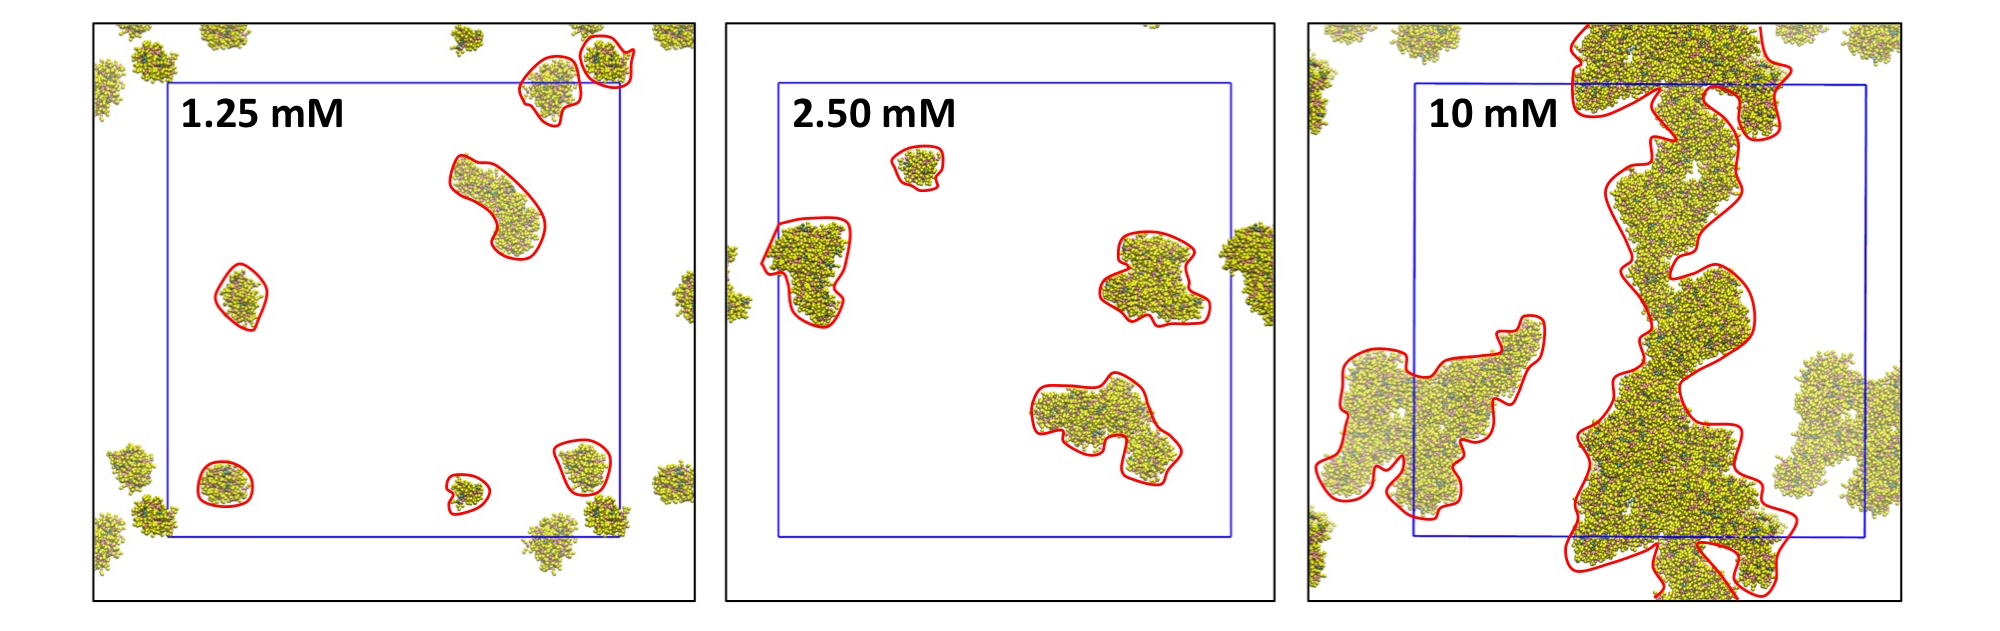
\includegraphics[width=0.95\linewidth]{3results_capsule/pics/final_SA.png} 
\caption[(SI) Self-assembly simulations, final configurations]{Final configurations obtained from 10 $\mu$s standard MARTINI simulations of the self-assembly of capzip molecules, from random initial configuration, at different concentrations. Boundaries of the simuation box in blue; different clusters are circled in red (the remaining ones are periodic copies of the ones highlighted).}
\label{fig:SA_final}
\vspace{0.7cm}
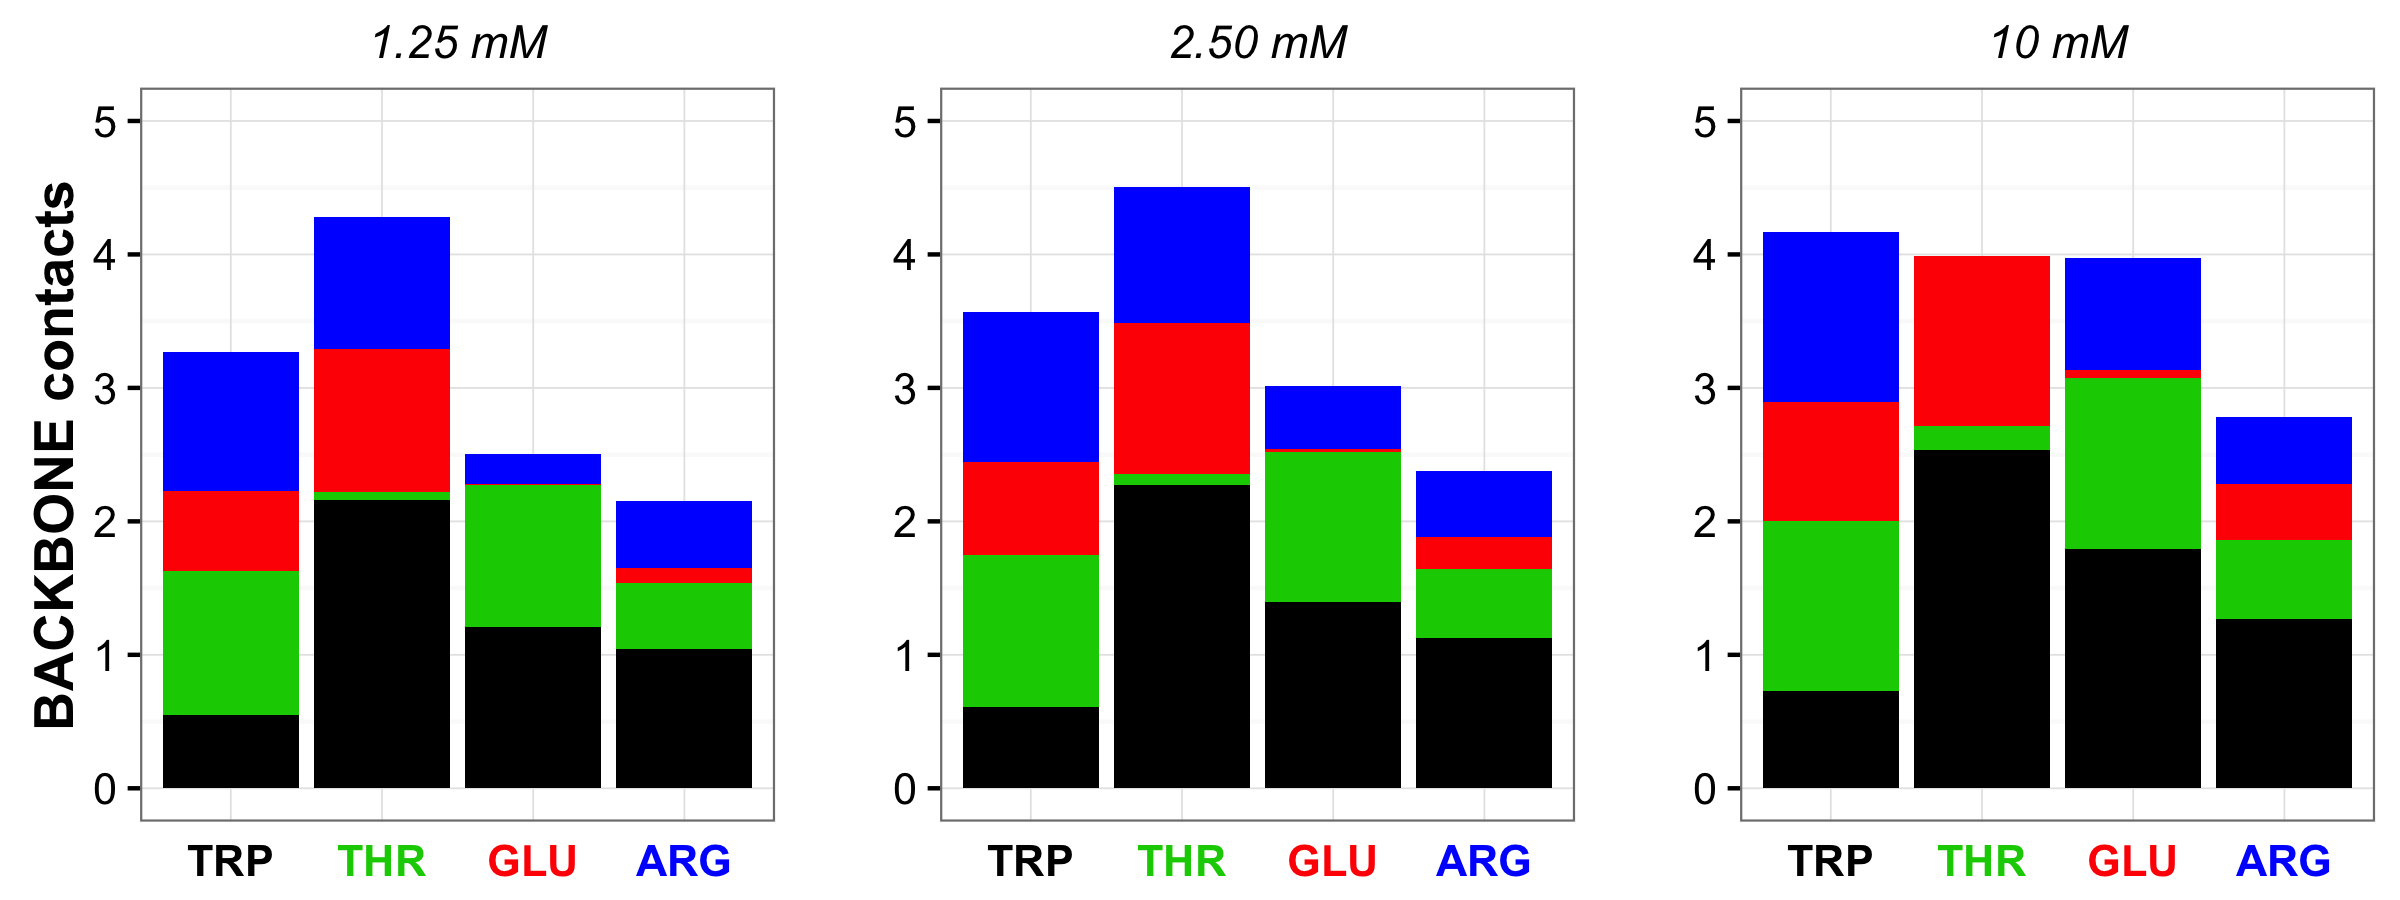
\includegraphics[width=0.95\linewidth]{3results_capsule/pics/contacts_SA.png} 
\caption[(SI) Self-assembly simulations: contacts]{Number of contacts per residue type in each arm of capzip for a MARTINI self-assembly simulations at different initial concentrations: each bar shows the average number for the residue on the $x$-axis; its color is split by the identity of the partner residue (color coded as in the $x$-axis legend). For mixed contacts the residue on the $x$-axis contributes with its backbone. Only contacts existing more than 50\% of the simulation time are considered.}
\label{fig:SA_contacts}
\vspace{0.7cm}
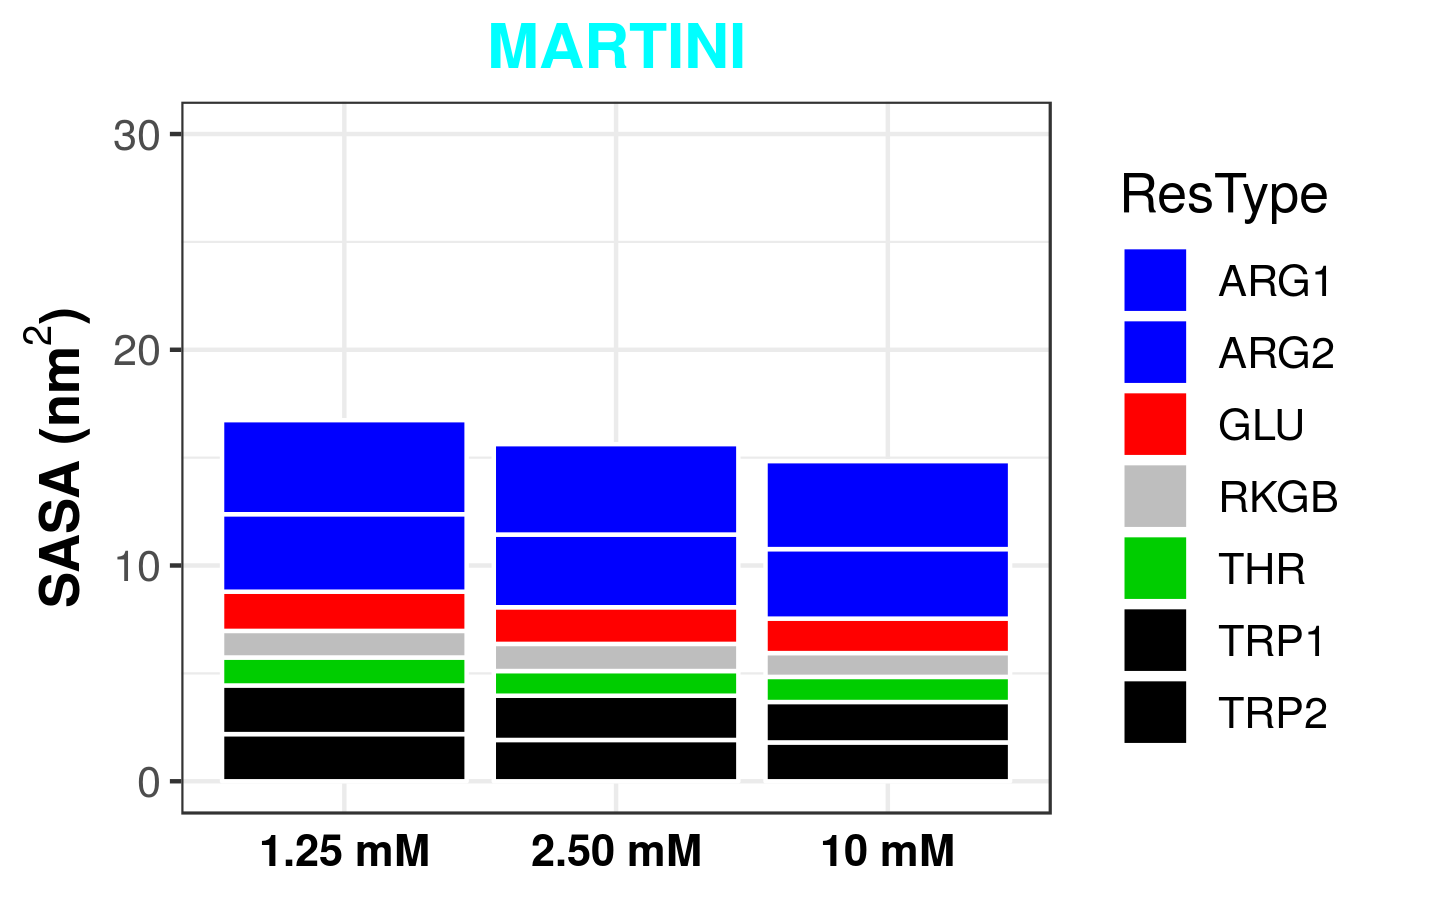
\includegraphics[height=0.3\linewidth]{3results_capsule/pics/st_SA_sasa_fractions.png} \label{fig:SA_sasa}
\caption[(SI) Self-assembly simulations: SASA]{Solvent Accessible Surface Area (SASA) per molecule, divided by residue types, for self-assembly simulations at different concentrations.}
\label{fig:SA_sasa_all}
\end{figure}

The two properties we want to assess from these simulations are the contacts between the molecules, classified by amino acid type, and the SASA of each residue type, to be compared with the results from the capsule model. However, from the previous simulations we also know that the MARTINI parametrisation promotes a very tight assembly of the molecules once they get in proximity, and that this is partially reverted back when backmapping a structure to an atomistic description. Therefore, the results from self-assembly simulations must be interpreted with the caveat that the protein-protein interactions might be overestimated.

The backbone contacts (Figure \ref{fig:SA_contacts}) show between 3 and 4 contacts per residue, which is about three times higher than the figure obtained for the ordered capsule structure (Figure \ref{fig:BTI_cont}), in line with a densely packed assembly.
%
Furthermore, there is a slight increase with the concentration.

The pattern of contacts suggests that Threonine interact with most partners. Interestingly, the contacts are distributed in a way which resemble more the atomistic pattern found for the capsule rather than the MARTINI one. In general, this confirms the role of the hydrophobic residues in keeping the assembly compact, but also suggests aggregation of molecules when a high concentration is simulated.

Regarding SASA values (Figure \ref{fig:SA_sasa_all}), they confirm what found also in the capsule conformation, with Arginine being exposed and Tryptophan buried. The SASA is decreasing with the concentration, as for low concentration several clusters are formed and float in solution separately (up to the time scale simulated), while for higher concentrations the molecules can merge in fewer larger clusters, which have less exposed surface.
%
Interestingly, the decrease in SASA and increase in contacts does not scale linearly with the concentration, as expected when the systems reach saturation and the clusters cannot favourably accommodate more molecules. However, as only three concentrations were simulated here, the data are not enough to extract a more precise dependence between these properties.

Again, when interpreting these results, one must remember that a backmapping to an atomistic resolution would produce more expanded structures, as it was observed for the capsule. However, also at the experimental level, high concentrations (of the order of mM as the ones simulated here) resulted in aggregation, i.e.\ the appearance of amorphous aggregates rather than geometrical capsules (data not shown). The MARTINI simulations are likely capturing this behaviour, and one would need a long simulation of a diluted solution to observe an ordered assembly. As it is almost impossible to simulate the micromolar regime used in experiments, the simulations of pre-assembled structures, as the ones presented previously in this chapter, are, so far, the only ones able to explore the relevant range of concentrations.

\subsection{On the long range electrostatic cut off in lipid simulations}
In a few paragraphs of this chapter we compare the simulations run here with the ones from the parametrisation work in the next chapter. As the reader will see, these are run on 512-lipid bilayers, with a simulation set up very similar to the one employed here.

However, the long range electrostatic are treated with a Reaction Field scheme and cut off radius of 1.4 nm. This choice was performed for consistency with previous parametrisation work.
%
Instead, the simulations run in the present chapter are run either with the Reaction Field and a cut off of 1.2 nm (512-lipid bilayers) or with a Particle Mesh Ewald treatment, and the same cut off (740-lipid bilayers).

Although briefly mentioned in the body of the chapter, we want to reiterate that these discrepancies might affect the simulations, but in measure smaller than the peptide or the electric field, which effect we wanted to assess.

Indeed, extensive literature on the effects of long range electrostatic treatment suggests that electrostatics have an influence on the ApL up to 0.010-0.015 nm$^2$ only. This is confirmed for the change in the cut off treatment (single or double) \citep{Silva2018,Reisser2017}, and the switch from PME to RF [\citet{Poger2012}; Table 1 in Chapter \ref{chapter:lip_par}].
%
The only conditions which severely affects the ApL seems the complete neglect of the long range electrostatic, choosing a plain cut off scheme \citep{Patra2003}.

Regarding the different cut off values, we did not find previous work testing the difference. The effect of the cut off is to discriminate which regions are treated in the exact way (nearby the atom for which the electrostatic force acting on it needs to be computed) and which instead through the long range approximation of choice (far away ones). As these approximations seem consistent among them and robust, we foresee that a small shift in the cut off length does not have a high impact on the simulation outcome.


\subsection{Buckyball simulations: results from Replica 2}

In the following pages we include the results obtained from Replica 2 of the buckyball bilayer and monolayer simulations (analogous to Figures \ref{fig:struct_UA_SIhere}-\ref{fig:BTI_sasa_exposed} and \ref{fig:eng_cg}-\ref{fig:mono_bi_sasa}).

\begin{figure}[p]
\centering
\subbottom[]{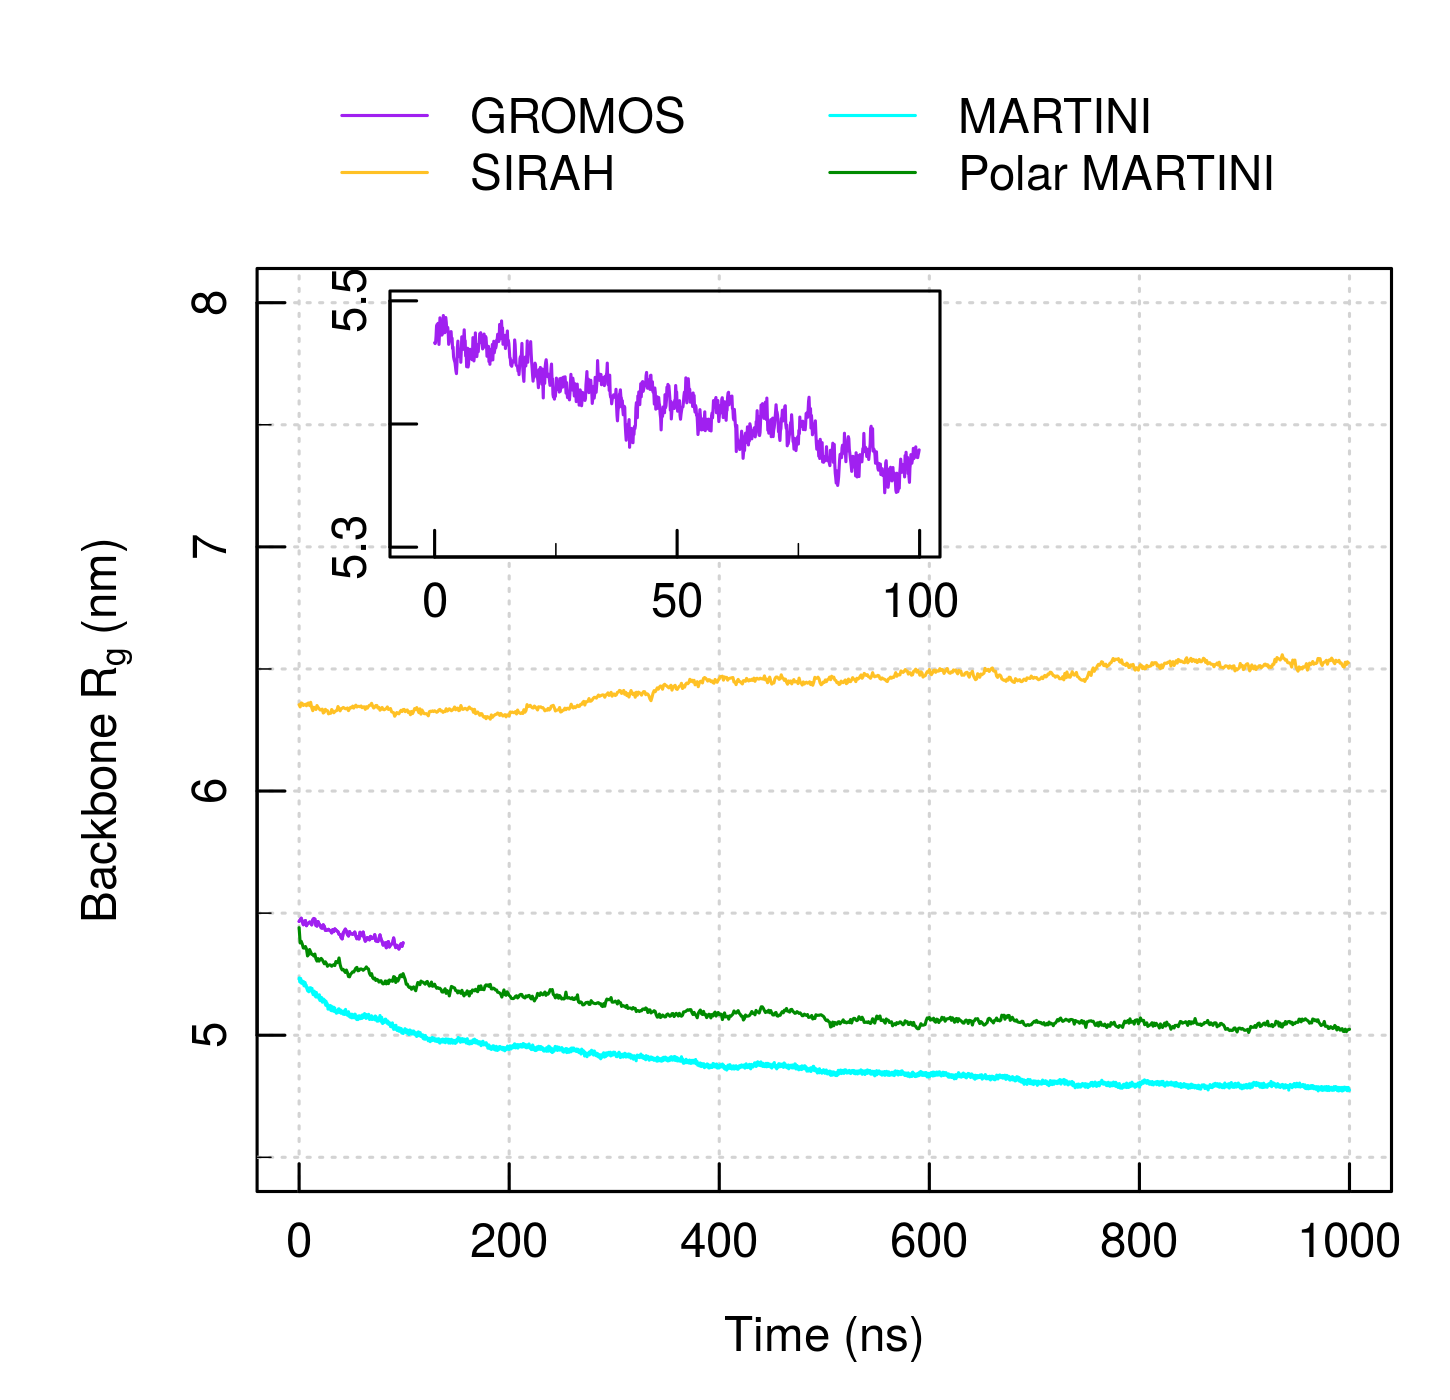
\includegraphics[width=0.48\linewidth]{3results_capsule/pics/R2_Rg_all.png}} 
\subbottom[]{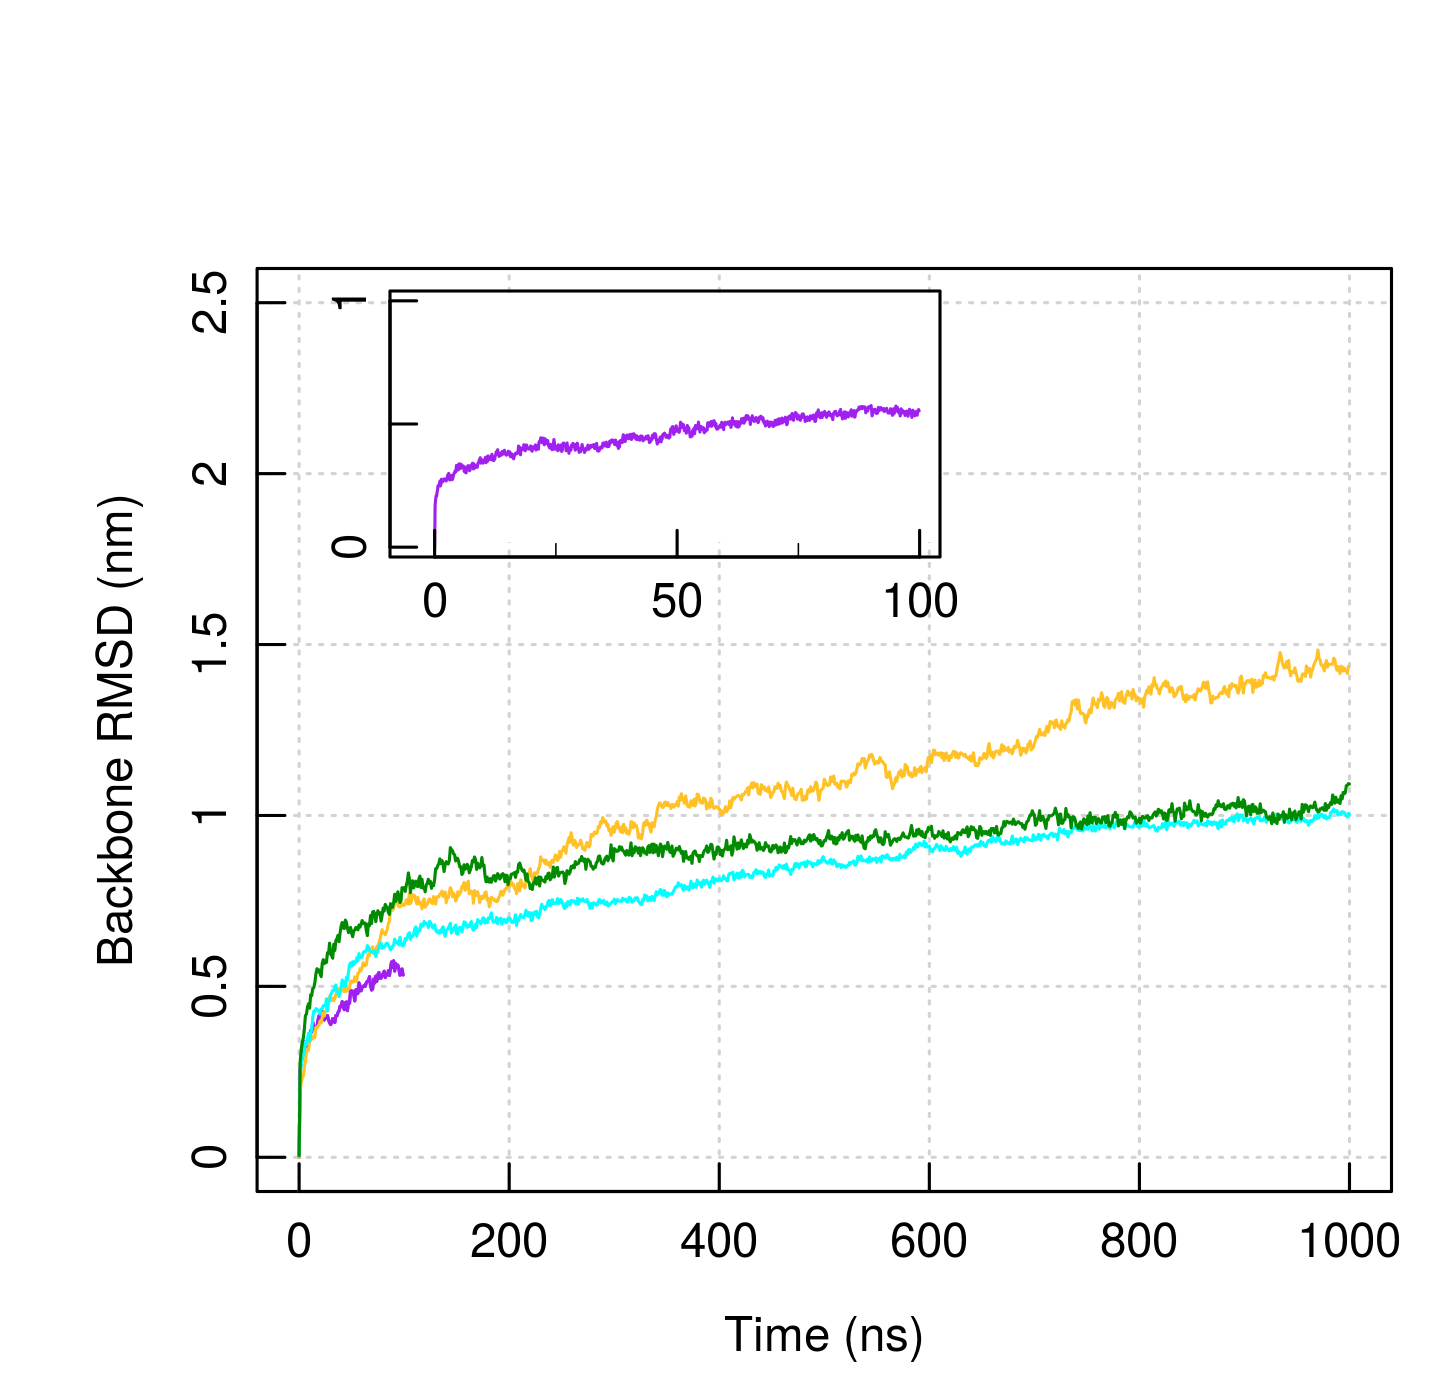
\includegraphics[width=0.48\linewidth]{3results_capsule/pics/R2_RMSD_all.png}} \\
\subbottom[]{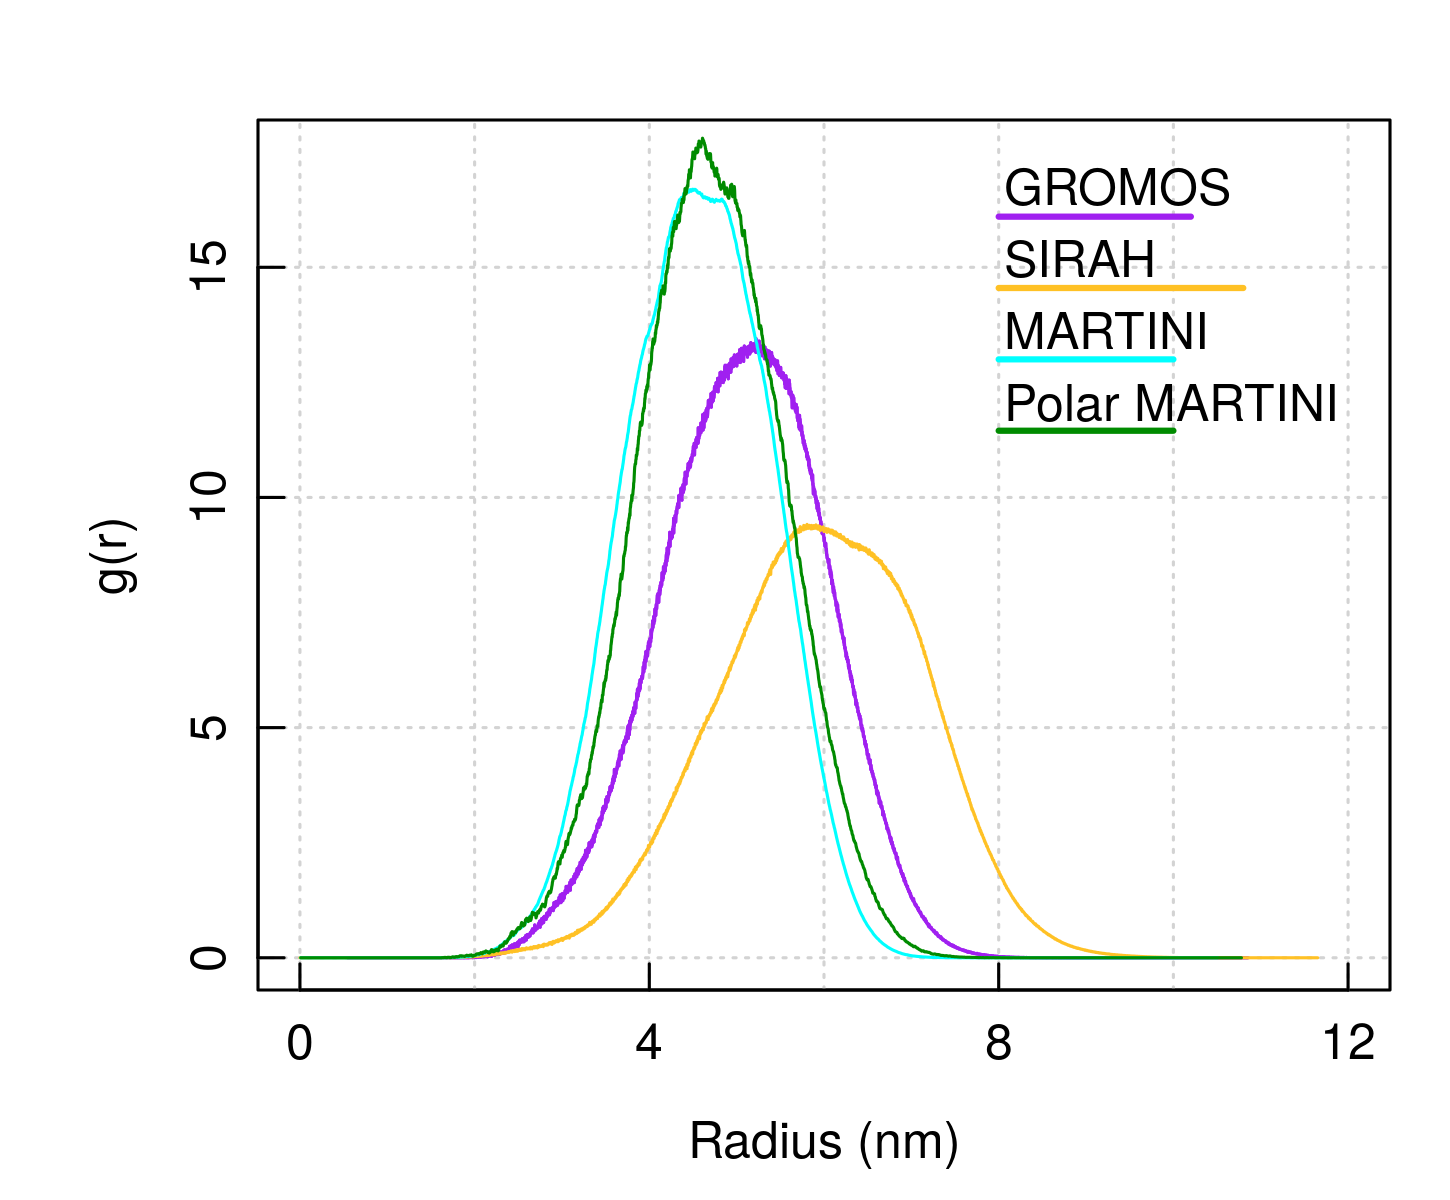
\includegraphics[width=0.48\linewidth]{3results_capsule/pics/R2_RDF_all.png}}
\caption[(SI) Replica 2: Structural measures on buckyball in solution]{(a) R$_g$ and (b) RMSD computed on the Protein backbone. Results are displayed for simulations performed in GROMOS (100 ns), SIRAH, MARTINI and MARTINI with polar water (all 1 $\mu$s). Inset: zoom on the GROMOS values. (c) RDF of Protein masses around their center of mass, computed on both layers, displayed for the same simulation set up as in (a,b). For each label of the legend, the bar has length of the respective FWHM of the Gaussian function fitting the data (thickness estimate). Results for Replica 2 of each simulation set-up.}
\label{fig:struct_UA_SIhere2}
\end{figure}

\begin{figure}[t]
\centering
\includegraphics[width=0.95\linewidth]{3results_capsule/pics/R2_RKGBcorr_boxplot_all.png} 
\caption[(SI) Replica 2: Correlation of motion between molecules of the buckyball]{Distribution of the correlation of motion between different molecules in the buckyball simulations. Black band: median of the distribution; box: first and third quartiles; whiskers: maximum and minimum, outliers excluded (hollow dots). Results for Replica 2 of each simulation set-up.}
\label{fig:BTI_corr2}
\end{figure}

\begin{figure}[t!]
\centering
\includegraphics[width=0.85\linewidth]{3results_capsule/pics/R2_stAll_beta_90_R1.png}
\caption[(SI) Replica 2: Arm pairing during simulations of the buckyball]{Number of paired arms within the same layer and between layers. Cut off distance between arms center of mass equal to 1.2 nm. Only contacts existing more than 90\% of the simulation time are counted. Results for Replica 2 of each simulation set-up.}
\label{fig:BTI_beta2}
\end{figure}

\begin{figure}[p!]
\centering
\includegraphics[width=0.95\linewidth]{3results_capsule/pics/R2_new_rep1_allFF.png}
\caption[(SI) Replica 2: Contacts between buckyball molecules]{Number of contacts per residue type in each arm of capzip: each bar shows the average number for the residue on the $x$-axis; its color is split by the identity of the partner residue (color coded as in the $x$-axis legend). For mixed contacts the residue on the $x$-axis contributes with its backbone. The parametrisation is reported along the $y$-axis. Only contacts existing more than 50\% of the simulation time are considered. Results for Replica 2 of each simulation set-up.}
\label{fig:BTI_cont2}
\end{figure}

\begin{figure}[t]
\centering
\includegraphics[width=0.85\linewidth]{3results_capsule/pics/R2_Hb_all.png} 
\caption[(SI) Replica 2: Hydrogen bonds in the buckyball molecule]{Average number of hydrogen bonds per residue occurring between amino acids, including the central scaffold RKGB, for a 100 ns atomistic simulation of the buckyball in solution. For each bar, the residue on the $x$-axis is the acceptor, and the bar is split by the identity of the donors. In the case of Backbone - Side chain and Side chain - backbone, the first mentioned correspond to the acceptor (and thus the residue on the $x$-axis). Results for Replica 2.}
\label{fig:BTI_hbonds2}
\end{figure}

\begin{figure}[t]
\centering
\subbottom[]{\includegraphics[height=0.3\linewidth]{3results_capsule/pics/R2_st_All_sasa_fractions.png}} 
\subbottom[]{\includegraphics[height=0.3\linewidth]{3results_capsule/pics/R2_st_Qsasa.png}} 
\caption[(SI) Replica 2: SASA per residue of a buckyball in solution]{(a) Solvent Accessible Surface Area (SASA) per molecule, divided by residue types. (b) Normalised SASA over the reference SASA computed for each amino acid type X as the value in a Gly-X-Gly tripeptide. Results for Replica 2 of each simulation set-up.}
\label{fig:BTI_sasa_exposed2}
\end{figure}

\begin{figure}[h!]
\centering
\vspace{3cm}
\subbottom[]{\includegraphics[width=0.8\linewidth]{3results_capsule/pics/R2_many_energies_brief.png}} 
\subbottom[]{\includegraphics[width=0.8\linewidth]{3results_capsule/pics/R2_ratio_energies_brief.png}} 
\caption[(SI) Replica 2: Non-bonded protein energy contribution to capsule structures]{(a) Protein-Protein and Protein-Water non-bonded interactions, normalised per molecule. Values obtained as average on the second half of the trajectory of Replica 2 for each set-up. (b) Ratio between the Protein-Protein and Protein-Water interactions for each force field, for Coulomb and Lennard-Jones respectively; or between Coulomb and Lennard/Jones, for Protein-Protein an Protein-Water interactions separately (note the log scale on $y$). Values computed as for plot (a). Points are misaligned along $x$ to facilitate the reading.}
\label{fig:eng_cg2}
\vspace{3cm}
\end{figure}


\begin{figure}[h!]
    \subbottom[]{\includegraphics[width=0.48\linewidth, align=c]{3results_capsule/pics/R2_compare_MonoBi_rmsd_init.png}}
    \subbottom[]{\includegraphics[width=0.48\linewidth, align=c]{3results_capsule/pics/R2_compare_MonoBi_RDF.png}}
    \caption[(SI) Replica 2: Comparison of monolayer and bilayer structural properties]{(a) RMSD of the monolayer and bilayer structures for SIRAH and Polar MARTINI force field, with respect to the initial geometrical configuration (external layer of Figure \ref{fig:BTI_vmd}, E). (b) RDF of Protein masses around their center of mass. For each label of the legend, the bar has length of the respective RDF FWHM (thickness estimate). Results for Replica 2 of each simulation set-up.}
\label{fig:mono_bi2}
\end{figure}

\begin{figure}[t!]
\centering
\subbottom[]{\includegraphics[width=0.48\linewidth]{3results_capsule/pics/st_sasaRes_mono_bi_init_bars.png}} 
\subbottom[]{\includegraphics[width=0.48\linewidth]{3results_capsule/pics/R2_st_sasaRes_mono_bi_bars.png}} 
\caption[(SI) Replica 2: SASA per residue of monolayer and bilater]{Solvent Accessible Surface Area (SASA) per molecule, divided by residue types for simulations of the bilayer and monolayer structure. (a) SASA computed from the initial configuration; (b) from the average over the production run. Results for Replica 2 of each simulation set-up.}
\label{fig:mono_bi_sasa2}
\end{figure}

\clearpage


\subsection{Additional Figures and Table}
\begin{figure}[h!]
\centering
\vspace{2.5cm}
\includegraphics[width=0.5\linewidth]{3results_capsule/pics/penta_final.png}
\caption[(SI) Pentagonal subunit atomistic simulation: final configuration]{Final configuration from a 100 ns simulation of the pentagonal subunit in solution. Bonds and cartoon representation, coloured by name. [VMD software, \citet{HUMP96}]}
\label{fig:penta_results_SI}
\end{figure}

\begin{figure}[h!]
\centering
\vspace{1cm}
\includegraphics[width=0.6\linewidth]{3results_capsule/pics/mindist_dlpc_MARTINI.png}
\caption[(SI) Minimal distance buckyball bilayer - DLPC membrane (MARTINI)]{Minimal distance between the buckyball bilayer and a DLPC membrane (using the pair of closest atoms) during a MARTINI simulation.}
\label{fig:mindist_buck_dlpc}
\end{figure}

\begin{figure}[h!]
\centering
\includegraphics[width=0.6\linewidth]{3results_capsule/pics/msd_MARTINI.png}
\caption[(SI) Typical lipid lateral MSD profile in MARTINI simulations.]{Typical lipid lateral MSD profile computed on Polar MARTINI simulations: MSD computed on the PO4 bead of DLPC for a 2880 lipids membrane, with an externally applied electric field of 20 mV/nm.}
\label{fig:MSD_martini}
\end{figure}

\begin{figure}[h!]
\centering
\vspace{1cm}
\scriptsize
 \def\arraystretch{1.6}
\begin{tabular}{lccccc}
 \multicolumn{6}{c}{\small \textbf{Table of simulations of pure membranes (atomistic)}} \\
  \hline
 Lipids & Box (nm) & E (mV/nm) & ES & $\,$Time (ns)$\,$ & Rep. \\
 \hline
 \multicolumn{6}{c}{\textbf{United atom GROMOS (GR)}} \\
 512 (b) & 12 & 0, 70, 120 	& RF & 400 							& 1$^a$ \\
 512 (b) & 12 & 130 			& RF & 600 							& 3$^a$ \\
 512 (b) & 12 & 140 			& RF & 150$^{P}$, 154$^{P}$, 200 	& 3$^a$ \\
 512 (b) & 12 & 140 			& RF & 200 							& 1$^b$ \\
 740 (b) & 14 & 0, 20		& PME & 400 							& 1$^b$ \\
 748 (m) & 14 & 0			& PME & 400							& 1$^b$ \\
 748 (m) & 14 & 130 			& PME & 20$^{P}$, 28$^{P}$, 39$^{P}$ & 3$^b$ \\
 \hline
 \multicolumn{6}{c}{\textbf{Coarse-grained Polar MARTINI (MA\_P)}} \\
 2880 (b) & 30 & 0, 20, 40 & PME & 500 & 1 \\
 2888 (m) & 30 & 0, 20, 40 & PME & 500 & 1 \\
 \hline
 \multicolumn{6}{c}{\textbf{Coarse-grained MARTINI (MA)}} \\
 720 (b) & 30 & 0 & RF & 1000 & 1 \\
 722 (m) & 30 & 0 & RF & 1000 & 1 \\
 \hline
\end{tabular}
\vspace{0.5cm}
\captionof{table}[Control simulations of pure membranes]{Table of control atomistic simulations of membranes. All run at 150 mM concentration of NaCl. 
%
Lipids: number of lipids, (b) bacterial model (DLPC/DLPG 3:1) and (m) mammalian model (DLPC).
%
Long-range electrostatic (ES): RF Reaction Field \citep{Tironi1995}, PME Particle Mesh Ewald \citep{Essmann1995}.
%
For the GROMOS force field (FF): $^a$ version 54a7 \citep{Schmid2011}, $^b$ 54a8 \citep{Reif2012}; coarse-grained MARTINI \citep{Marrink2007, Monticelli2008}, coarse-grained MARTINI with polar water \citep{Yesylevskyy2010}.
%
Superscript P in the time length denotes observation of poration.}
\label{table:SI_membrane}
\end{figure}
